Una volta discussa l'interazione della radiazione con la materia, siamo pronti per discutere i rivelatori. Prima di andare a discutere nel dettaglio le diverse tipologie di rivelatore, andiamo a presentare alcune proprietà generali. Infatti, nonostante nel corso degli anni siano state sviluppate diverse tipologie di rivelatori che sfruttano meccanissimi diversi, hanno elettronica differente ecc., ci sono dei concetti di base che sono validi per tutti i rivelatori.

\section{Che cos'è un rivelatore}

Un rivelatore si può definire come uno strumento che viene usato per rivelare il passaggio di una particella o di una radiazione.

I rivelatori non sono tutti gli stessi, ce ne sono di diverse tipologie aventi diverse funzionalità ulteriori a quella di rivelare il passaggio di una particella: alcuni sono in grado di misurare l'energia della particella oppure tracciarla, quindi andare ad individuare il percorso seguito della particella o addirittura in alcuni casi identificarla, quindi capire che tipo di particella è passata attraverso di esso. Tuttavia, indipendentemente dalle diverse tipologie di rivelatori, è essenziale che un principio di base sia rispettato: affinché un rivelatore possa rivelare una particella o una radiazione, è fondamentale che queste interagiscano con il rivelatore stesso attraverso uno dei meccanismi che abbiamo discusso in base al tipo di particella o di radiazione che stiamo andando a considerare.

Come abbiamo studiato, l'interazione tra particelle e materiali dipende dalla sezione d'urto dei vari processi, che a sua volta è influenzata dalle caratteristiche della particella incidente e del materiale assorbitore. Per questo motivo, è essenziale comprendere come variano le sezioni d'urto nei diversi processi per capire le scelte progettuali dei rivelatori, come la geometria, i materiali utilizzati e le prestazioni ottenibili. Quando si progetta un rivelatore, bisogna considerare che, sebbene possa essere ottimizzato per rivelare certi tipi di particelle, ciò comporterà inevitabilmente delle limitazioni. Ad esempio, un rivelatore concepito per particelle cariche potrebbe non essere adatto per la radiazione elettromagnetica. Inoltre, il materiale con cui è costruito determinerà l'efficienza del rivelatore in relazione al tipo di particelle e alla loro energia.

Un aspetto fondamentale nella rivelazione è il \textit{tempo di interazione}. Questo rappresenta il tempo necessario per arrestare una particella o per lo sviluppo di uno sciame. I tempi di interazione sono estremamente brevi, dell'ordine dei nanosecondi nel caso di un materiale gassoso e dei picosecondi nel caso di un materiale solido. Oltre a questi, bisogna considerare anche il tempo che impiega il rivelatore per raccogliere il risultato dell'interazione, che chiaramente varia a seconda del meccanismo di interazione.

Il risultato netto dell'interazione delle radiazioni in un'ampia categoria di rivelatori è la comparsa di una determinata quantità di carica elettrica di ionizzazione $Q$ all'interno del volume attivo del rivelatore\footnote{Il volume attivo di un rivelatore è quella parte del rivelatore stesso in cui avviene l'effettiva rivelazione delle radiazioni, ovvero dove le particelle interagiscono con il materiale del rivelatore producendo segnali rilevabili, come la creazione di cariche elettriche, scintillazioni, o altri fenomeni misurabili.}. Successivamente, questa carica deve essere raccolta per formare il segnale elettrico di base. Tipicamente, la raccolta della carica viene realizzata attraverso l'imposizione di un campo elettrico all'interno del rivelatore, che provoca lo spostamento delle cariche positive e negative create dalla radiazione in direzioni opposte, producendo così un segnale in uscita. Il tempo necessario per raccogliere completamente la carica varia notevolmente da un rivelatore all'altro; in generale, questi tempi di rivelazione sono leggermente più lunghi rispetto ai tempi di interazione: vanno dai nanosecondi ai microsecondi, ma possono arrivare anche all'ordine del millisecondo nel caso di rivelatori molto lenti. Man mano che affronteremo i diversi tipi di rivelatore, esamineremo anche questi tempi di risposta, ovvero i tempi di rivelazione.

\section{Modi di operazione}

Il modo in cui operano la maggior parte dei rivelatori è quello di dare luogo a un segnale\footnote{Questo segnale nella pratica è un impulso di corrente. Nel seguito la professoressa parla di questi segnali come segnali di tensione, ma credo siano equivalenti data la legge di Ohm. In ogni caso, il Knoll ne parla in \S4.2.C\,.} ogni qualvolta vengono attraversati da una particella o da una radiazione. Fanno eccezione una classe di rivelatori che potremmo definire come rivelatori visualizzanti o traccianti, i quali funzionano semplicemente visualizzando il passaggio delle particelle, cioè permettono di visualizzare il passaggio di una particella senza però avere un segnale in uscita in corrispondenza del passaggio della particella o della radiazione. Degli esempi sono le emulsioni nucleari, che possiamo immaginarle come delle lastre fotografiche che visualizzano la traccia di una particella, oppure le camere a bolle e le camere a nebbia.

Concentriamoci sui rivelatori che segnalano il passaggio di una particella attraverso la formazione di un segnale elettrico.

\begin{figure}[H]
   \centering
   \begin{tikzpicture}
      \draw[->] (0,0) -- (9,0) node[right] {$t$};
      \draw[->] (0,0) -- (0,4) node[above] {$i(t)$};
      \draw[thick, red] (0,0) -- (1,0) arc (-90:0:0.2cm) -- (1.2,1.3) arc (180:90:0.2cm) -- (1.8,1.5) arc (90:0:0.2cm) -- (2,0.2) arc (180:270:0.2cm) -- (3,0) arc (-90:0:0.2cm) -- (3.2,2.8) arc (180:90:0.2cm) -- (3.8,3) arc (90:0:0.2cm) -- (4,0.2) arc (180:270:0.2cm) -- (6,0) arc (-90:0:0.2cm) -- (6.2,1.8) arc (180:90:0.2cm) -- (6.8,2) arc (90:0:0.2cm) -- (7,0.2) arc (180:270:0.2cm) -- (8,0);
    \end{tikzpicture}
\end{figure}

Ogni segnale avrà caratteristiche specifiche. Innanzitutto, si manifesteranno a intervalli temporali variabili, cioè, a meno che non si tratti di un fenomeno periodico, i tempi tra un evento e il successivo saranno casuali. Ciè è dovuto al fatto che l'arrivo e la rilevazione di particelle emesse da una sorgente radioattiva sono fenomeni casuali governati dalla statistica di Poisson, il che implica che l'intervallo temporale tra due eventi consecutivi non è fisso, ma cambia di volta in volta. Ciononostante, questa variazione segue una distribuzione che ha un andamento esponenziale decrescente.

La distanza tra due eventi consecutivi può variare notevolmente a seconda del fenomeno che si sta studiando e del tipo di radiazione rivelata. Ad esempio, se si dispone di una sorgente quasi esaurita con un'attività molto bassa, i segnali potrebbero verificarsi con una frequenza molto bassa; al contrario, in altri tipi di fenomeni, la frequenza di conteggio potrebbe essere molto più elevata. Per questo motivo i modi in cui un rivelatore può operare sono principalmente due:

\begin{itemize}
   \item \textit{Pulsed mode}: il rivelatore rivela singoli impulsi in quanto questi arrivano in tempi abbastanza distanziati l'uno dall'altro, per cui è possibile studiare l'arrivo della singola particella/radiazione. Un esempio di fenomeno che si studia utilizzando un rivelatore in pulsed mode è la misura dell'arrivo di particelle della radiazione cosmica mediante un contatore Geiger: ogni volta che arriva una particella, questo emette un bip e viene prodotto un segnale, quindi è possibile contare singolarmente i diversi impulsi.
   \item \textit{Current mode}: quando gli impulsi sono molto ravvicinati in tempo, quindi abbiamo un'alta frequenza di conteggi, il rivelatore non riesce più a distinguere tra i singoli impulsi e lavorerà nella cosiddetta current mode, cioè nella modalità corrente. Quello che si va a misurare in questa modalità è sostanzialmente una corrente media.
\end{itemize}

In laboratorio lavoreremo principalmente in pulsed mode.

Chiariamo meglio che cos'è un segnale. Per segnale si intende una differenza di tensione, che quindi può essere visualizzato grazie a uno oscilloscopio.

\begin{figure}[H]
   \centering
   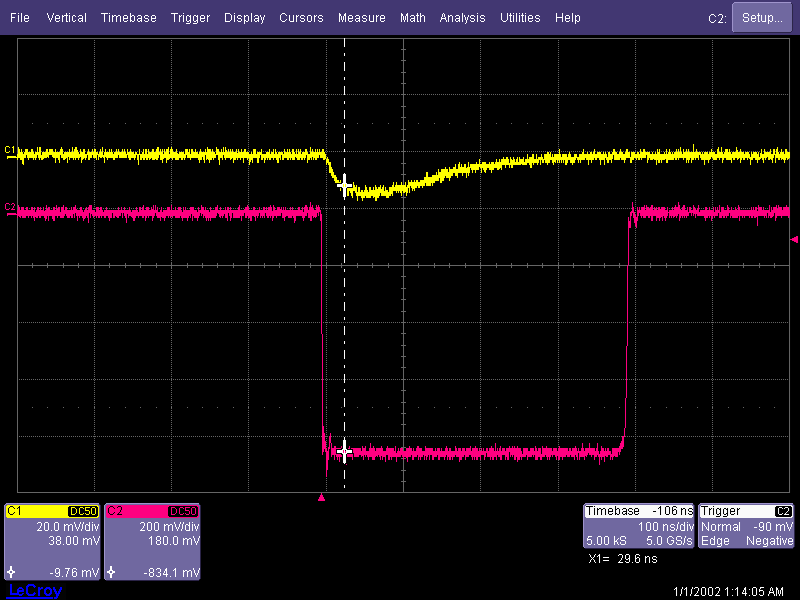
\includegraphics[width=0.7\textwidth]{immagini/segnali_rivelatori.png}
\end{figure}

Nella figura è mostrata la schermata di un oscilloscopio digitale, che consente di visualizzare più segnali contemporaneamente. Sull'asse orizzontale viene rappresentato il tempo, in quello verticale la tensione.

In questo caso, sono rappresentati due segnali distinti: uno in giallo e uno in rosa. Questi segnali, pur essendo molto diversi tra loro, hanno in comune la caratteristica di essere impulsi. Si nota infatti come, a partire da un valore di tensione costante (detto baseline), si verifichi una variazione nella tensione che persiste per una certa durata. Successivamente, il valore della tensione ritorna al livello iniziale.

Pur essendo questa caratteristica comunque ad entrambi i segnali, essi sono molto differenti. Il segnale giallo è un segnale analogico, la cui ampiezza può variare in modo continuo. Attualmente stiamo osservando un impulso specifico, ma un futuro impulso, causato da una nuova particella o radiazione, potrebbe avere un'ampiezza leggermente diversa, mantenendo però la stessa forma generale. Ciò che cambia è l'ampiezza del segnale, ossia la distanza tra la baseline e il valore massimo raggiunto. Questa ampiezza può quindi assumere valori differenti in modo continuo.

Al contrario, il segnale rosa ha una forma completamente diversa: è squadrato (onda quadra) e ha una durata che, in questo caso, viene spesso determinata dall'utente o dall'elettronica utilizzata. In questo contesto, non ci concentriamo sulla durata del segnale, ma piuttosto sul fatto che esso passa dalla baseline a un livello di tensione diverso, per poi ritornare alla baseline. Ad esempio, osservando la scala verticale, ogni divisione corrisponde a 200 mV, quindi questo segnale ha un'ampiezza di poco più di 800 mV. Si tratta di un segnale logico, che trasmette un'informazione limitata: indica semplicemente il passaggio dallo stato logico 0 allo logico 1, ma non fornisce altre informazioni. Se un nuovo impulso dovesse arrivare, avrebbe le stesse caratteristiche, con la stessa durata e ampiezza. Questo tipo di segnale è utile solo per contare il numero di impulsi ricevuti, senza poter estrarre ulteriori informazioni.

\subsection{Informazioni dai segnali}

Esistono diversi tipi di rivelatori che generano segnali differenti. Alcuni producono segnali logici, mentre altri emettono segnali analogici che trasportano informazioni aggiuntive sulla particella che possiamo dedurre dalle sue caratteristiche. Vediamo cosa possiamo dedurre.

\vspace{0.2cm}\textbf{Ampiezza}

Per ampiezza dei segnali intendiamo il valore massimo di tensione raggiunto dal segnale rispetto alla baseline. Essa può essere diversa a seconda dell'energia della particella incidente. Esistono infatti rivelatori che generano segnali la cui ampiezza è proporzionale all'energia depositata nel rivelatore stesso, risultando in un segnale più ampio quanto maggiore è l'energia depositata all'interno del rivelatore.

\E da notare che l'ampiezza del segnale puà variare anche per effetto delle fluttuazioni statistiche derivanti da altri fenomeni o a causa del rumore, per cui si ottiene un segnale di ampiezza leggermente diversa per motivi non fisici, nel senso che non è stata realmente depositata un'energia di valore diverso.

\vspace{0.2cm}\textbf{Tempo di arrivo}

Esso è il tempo associato al segnale e che fornisce informazioni sul tempo di arrivo della particella. Per capire quando il segnale è effettivamente arrivato è sufficiente andare a vedere l'istante in cui il segnale si discosta dalla baseline. Nel caso riportato in figura, notiamo come per le prime quattro suddivisioni della scala dei tempi (corrispondenti ciascuna a 100 ns) non c'è un segnale, in quanto abbiamo una tensione che è costante. Dopodiché all'improvviso parte un segnale dovuto appunto ad un impulso. Quand'è che parte l'impulso? Non è facile determinare l'inizio di questo segnale perché ci sono delle leggere fluttuazioni dovute al rumore elettrico, infatti la linea della tensione non è esattamente costante, bensì fluttua anche quando non c'è nessun impulso. In casi come questi si deve scegliere una sorta di soglia, cioè un livello di tensione superato il quale si può ritenere abbastanza ragionevole che effettivamente si stia presentando un segnale e non si tratti semplicemente di una fluttuazione. In tal caso, il tempo di inizio del segnale sarà dato dall'istante in cui si supera tale livello di soglia.

\vspace{0.2cm}\textbf{Forma e durata}

Oltre all'ampiezza, ci può interessare anche quanto dura il segnale. Ad esempio il segnale giallo raggiunge il suo valore massimo all'incirca a 50 ns dal suo iniziao, ma in realtà si esaurisce in 300 ns.

Ci può interessare anche la forma del segnale, ad esempio la discesa o la risalita. Infatti ci sono dei rivelatori che producono dei segnali che hanno forme diverse a seconda del tipo di particella che ha inciso, per cui a seconda che sia una particella carica o una radiazione elettromagnetica il segnale prodotto cambia forma e quindi se si è in grado di analizzare la forma del singolo segnale si può capire se il rivelatore ha misurato ad esempio una particella $\alpha$ o un $\gamma$ e quindi attraverso l'analisi della forma del segnale si può procedere a una sorta di identificazione, cioè capire effettivamente che particella è arrivata.

\section{Analisi delle ampiezze}

Nella maggior parte dei rivelatori che tratteremo, l'ampiezza ci darà informazioni sull'energia che sarà depositata dalla particella incidente sul rivelatore. Infatti, come abbiamo già detto, l'ampiezza del segnale dipenderà dall'energia depositata dalla particella/radiazione; nella maggior parte dei casi esiste una relazione lineare tra energia depositata e ampiezza del segnale prodotto, quindi se andiamo ad analizzare l'ampiezza del segnale in automatico sapremo quanta energia è stata depositata nel rivelatore. Questo processo equivale a fare un'analisi delle ampiezze, che tipicamente si fa rappresentando la distribuzione delle ampiezze degli eventi misurati. Solitamente tale distribuzione viene rappresentatata mediante una distribuzione differenziale $\dv*{N}{H}$, che è sostanzialmente un istogramma degli impulsi misurati, detto \textit{spettro delle ampiezze}.

\begin{approfondimento}[Lo spettro degli impulsi]
   \footnotesize
   Questo approfondimento è dovuto al fatto che secondo me è spiegato molto male il concetto di distribuzione delle ampiezze, per cui riporto quanto detto dal Knoll in \S4.2 "Pulse height spectra".

   \vspace{0.2cm}La distribuzione delle ampiezze degli impulsi è una caratteristica del segnale in uscita di un rivelatore che viene comunemente utilizzata per dedurre informazioni sulla radiazione incidente o sul funzionamento del rivelatore stesso.

   Il modo più comune di rappresentare le informazioni sulle ampiezze degli impulsi è attraverso la distribuzione differenziale delle altezze degli impulsi. Una distribuzione ipotetica a scopo di esempio è mostrata nel seguente grafico:
   \begin{figure}[H]
      \centering
      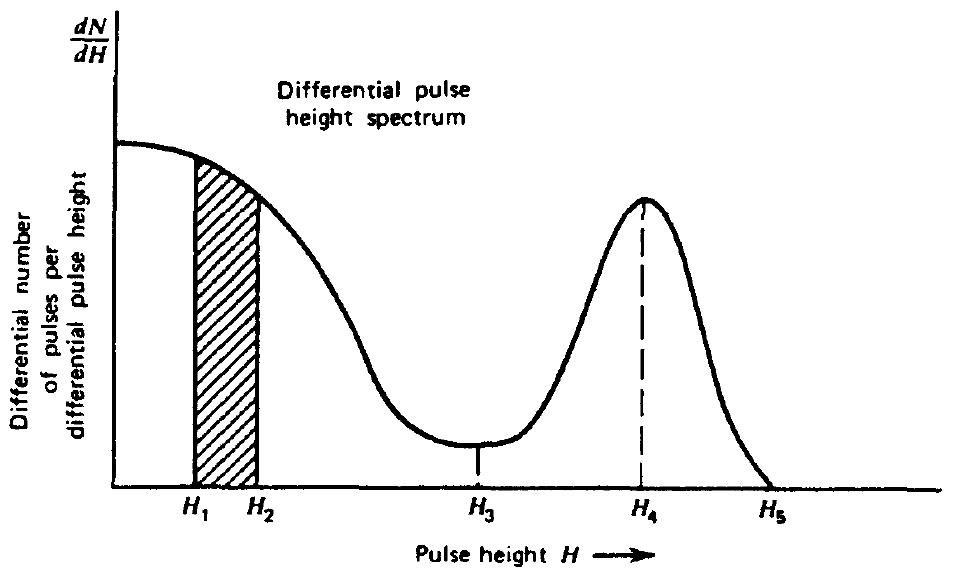
\includegraphics[width=0.6\textwidth]{immagini/distribuzione_differenziale_ampiezze.png}
   \end{figure}
   Sulle ascisse sono riportate le ampiezze degli impulsi con scala lineare, che va da zero a un valore più alto dell'ampiezza di qualsiasi impulso osservato dalla sorgente; l'ordinata rappresenta il numero differenziale $\dd{N}$ di impulsi osservati con un'ampiezza all'interno dell'incremento differenziale di ampiezza $\dd{H}$, diviso per tale incremento, o $\dv*{N}{H}$. La scala orizzontale ha quindi unità di ampiezza degli impulsi (Volt), mentre la scala verticale ha unità di ampiezza inversa (Volt$^{-1}$).
   
   Il numero di impulsi la cui ampiezza si trova tra due valori specifici, $H_1$ e $H_2$, può essere ottenuto integrando l'area sotto la distribuzione tra questi due limiti, come mostrato nell'area tratteggiata in figura.

   \begin{equation*}
      \text{Numero di impulsi con ampiezza tra $H_1$ e $H_2$}
      =\int_{H_1}^{H_2} \dv{N}{H} \dd{H}
   \end{equation*}
   
   Il numero totale di impulsi $N_0$ rappresentato dalla distribuzione può essere ottenuto integrando l'area sotto l'intero spettro:
   \begin{equation*}
      N_0=\int_{0}^{+\infty} \dv{N}{H} \dd{H}
   \end{equation*}
   La maggior parte degli utenti degli strumenti di rivelazione è abituata a osservare la forma della distribuzione differenziale delle altezze degli impulsi per identificare caratteristiche significative della sorgente degli impulsi. L'ampiezza massima degli impulsi osservata (nel nostro esempio pari ad $H_5$) è semplicemente il punto lungo l'ascissa in cui la distribuzione arriva a zero. I picchi nella distribuzione, come quello per $H_2$, indicano ampiezze di impulsi intorno a cui si trovano molti impulsi; viceversa, le valli o i punti bassi nello spettro, come $H_3$, indicano valori dell'ampiezza degli impulsi intorno ai quali si verificano relativamente pochi impulsi.
   
   %L'interpretazione fisica dell'altezza dello spettro differenziale degli impulsi coinvolge sempre aree sotto lo spettro tra due limiti dati di altezza degli impulsi. Il valore dell'ordinata stessa ($\dv*{N}{H}$) non ha significato fisico fino a quando non viene moltiplicato per un incremento dell'ascissa $H$.
\end{approfondimento}

\begin{esempio}[Distribuzione delle ampiezze per il $^{\text{137}}$Ce]\label{es:distr_ampiezze_cesio}
   In figura possiamo vedere un istogramma delle ampiezze, ottenuto utilizzando uno scintillatore con una sorgente di \ce{^{137}Ce} che emette $\gamma$ monoenergetici a 662 keV.

\begin{figure}[H]
   \centering
   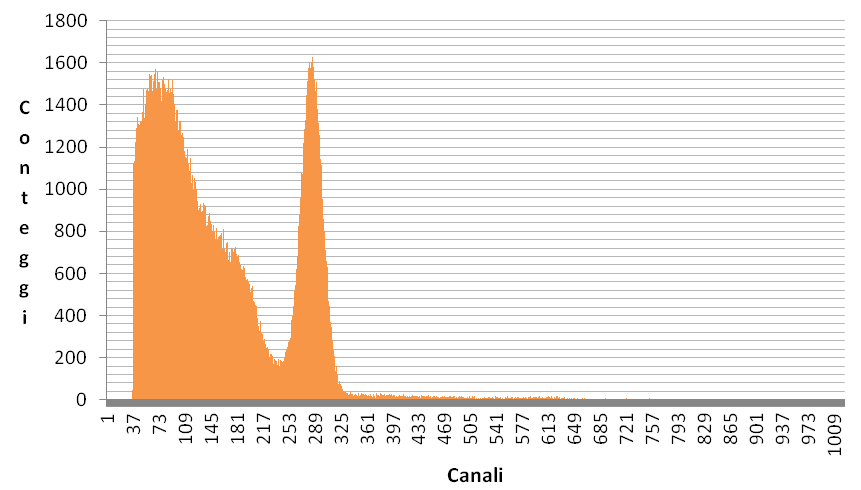
\includegraphics[width=0.615\textwidth]{immagini/distribuzione_ampiezze_impulsi_es_1.png}
\end{figure}

Quello che succede ad ogni interazione è che un $\gamma$ interagisce con il rivelatore, deposita una certa quantità della sua energia (che può essere tutta o anche solo una parte) e quindi in corrispondenza di ogni gamma si ottiene un segnale con una data ampiezza. Analizziamo allora questa distribuzione di ampiezze.

Se il $\gamma$ lasciasse ogni volta nel rivelatore tutta la sua energia, ci aspetteremmo di trovare sempre la stessa ampiezza, corrispondente nell'esempio a 662 keV. In realtà otteniamo uno spettro con una forma abbastanza complessa che ci dice che oltre a un valore di energia molto probabile e rappresentato dal picco in corrispondenza del canale 289, si presentano anche tanti eventi, quindi tanti $\gamma$, che rilasciano parte della loro energia, perché corrispondono a segnali di ampiezza più bassa. Il picco che vediamo è il cosiddetto picco fotoelettrico, cioè il picco che si ottiene quando il $\gamma$ interagisce per effetto fotoelettrico con lo scintillatore. Infatti in quel caso come prodotto dell'effetto fotoelettrico si ha un elettrone che ha assorbito tutta l'energia del fotone, il quale può percorrere pochi millimetri all'interno dell'elettrone prima di perdere tutta la sua energia. Quindi essenzialmente questi sono degli eventi in cui il gamma ha perso la sua energia per effetto fotoelettrico e l'ha trasferita all'elettrone e l'elettrone a sua volta rimane intrappolato all'interno del rivelatore perdendo tutta la sua energia attraverso i processi collisionali che abbiamo descritto in precedenza. In conclusione sono eventi in cui viene ricostruita tutta l'energia del $\gamma$ incidente. Ovviamente teoricamente dovremmo avere un delta di Dirac\footnotemark, ma nella realtà abbiamo un picco un po' più largo dovuto a effetti del rivelatore, che non è in grado esattamente di ricostruire l'energia con una precisione infinita, quindi abbiamo una sorta di risoluzione dettata dal rivelatore.

Tutti gli altri eventi che troviamo alla sinistra del picco, che prendono il nome di spalla Compton, corrispondono a dei casi in cui l'energia che viene rilasciata e depositata nello scintillatore è solamente una parte dell'energia del $\gamma$ incidente perché evidentemente sono avvenuti altri meccanismi\footnotemark. Si tratta infatti di effetti di scattering Compton, dove come prodotto finale si produce non solo un elettrone che chiaramente perderà la sua energia nello scintillatore, ma anche un fotone diffuso. Questo fotone ha una probabilità più bassa di interagire, quindi potrebbe fuggire dal rivelatore e non depositare la sua energia, ecco perché in questi eventi viene ricostruita solamente parte dell'energia che è quella dovuta all'elettrone scatterato durante l'effetto Compton. Abbiamo tanti valori di energia perché l'energia che viene assegnata al fotone diffuso e all'elettrone cambia a seconda dell'angolo di diffusione, quindi abbiamo uno spettro continuo di valori.

Chiaramente, se siamo interessati a sapere qual è l'energia del gamma, ci concentreremo sul picco fotoelettrico, in quanto corrisponde meglio all'energia del $\gamma$ di partenza.
\end{esempio}
\footnotetext{I $\gamma$ corrispondono a transizioni tra livelli nucleari, per cui non possono assumere qualsiasi valore di energia bensì hanno dei valori per precisi, corrispondenti alla differenza energetica dei livelli tra cui avviene la transizione.}
\footnotetext{Certamente non avvengono meccanismi di produzione di coppie perché stiamo parlando di gamma di 662 keV, quindi siamo al di sotto dell'energia di soglia}

L'esempio appena visto ci mostra come il segnale che viene tradotto dal rivelatore possa fornire informazioni sull'energia depositata nel rivelatore. Ribadiamo che quest'ultima non corrisponde sempre all'energia della particella emessa, ma potrebbe essere soltanto una parte, a seconda dei meccanismi che si sono verificati all'interno del rivelatore.

Vediamo che tipo di informazioni si possono estrarre da uno spettro:

\begin{itemize}[leftmargin=0.5cm]
   \item Potremmo essere interessati a sapere quanti segnali sono arrivati complessivamente nel tempo di misura, in modo da valutare quante particelle siamo riusciti a misurare. Ovviamente questo numero è legato all'attività della sorgente, quindi più questa è attiva, maggiore sarà il numero di eventi che riusciamo ad accumulare in un dato intervallo di tempo, e questo si può valutare realizzando l'integrale del spettro, quindi sommando sostanzialmente quanti eventi si trovano in ciascuno dei bin dell'istogramma;
   \item Potremmo essere interessati solamente a una pozione dello spettro, ad esempio potremmo voler analizzare soltanto gli eventi fotoelettrici, in modo da capire qual è la percentuale di eventi associati a tale fenomeno. Per fare ciò scegliamo degli estremi dello spettro e calcoliamo l'integrale dello spettro esteso solamente a tale regione;
   \item In base alla forma dello spettro possiamo individuare diverse regioni relative a particolari fenomeni, come nel caso della spalla Compton o del picco fotoelettrico. Inoltre possiamo andare a guardare il valore massimo delle ampiezze, quindi qual è la massima energia che viene misurata in questa tipologia di eventi.
\end{itemize}

\subsection{Calibrazione di uno spettro}

In laboratorio, un grafico del genere viene realizzato tramite un ADC, il quale traduce l'ampiezza del segnale in un numero che varia in un intervallo che dipende dal numero di bit a disposizione. Notiamo infatti come la distribuzione dell'\esref{es:distr_ampiezze_cesio} sia espressa in termini di canali, ossia in termini del numero prodotto dall'ADC. In particolare, nell'esperienza di laboratorio in cui adoperiamo uno scintillatore per misurare i $\gamma$ avremo a disposizione un ADC a 11 bit, il che vuol dire $2048$ numeri (da $0$ a $2047$). Nasce quindi la necessità di capire a che valore di energia corrisponde ciascun canale, e per fare ciò bisogna effettuare una calibrazione.

Per fare una calibrazione bisogna saper associare ciascun canale ad un valore di energia, quindi si utilizzano delle sorgenti note, di cui conosciamo i valori di energia adoperando delle sorgenti. Utilizzandone anche solamente due, come il cesio-137 che emette a 662 keV e il cobalto-60 che invece emette due $\gamma$ a due energie diverse, uno a 1117 keV e l'altro 1332 keV. La vicinanza di questi due valori fa sì che i due picchi fotoelettrici siano parzialmente sovrapposti, ma ciò è irrilevante in quanto ci interessa la possibilità di individuare il centroide del picco e di associarlo alla corretta energia.
\begin{figure}[H]
   \centering
   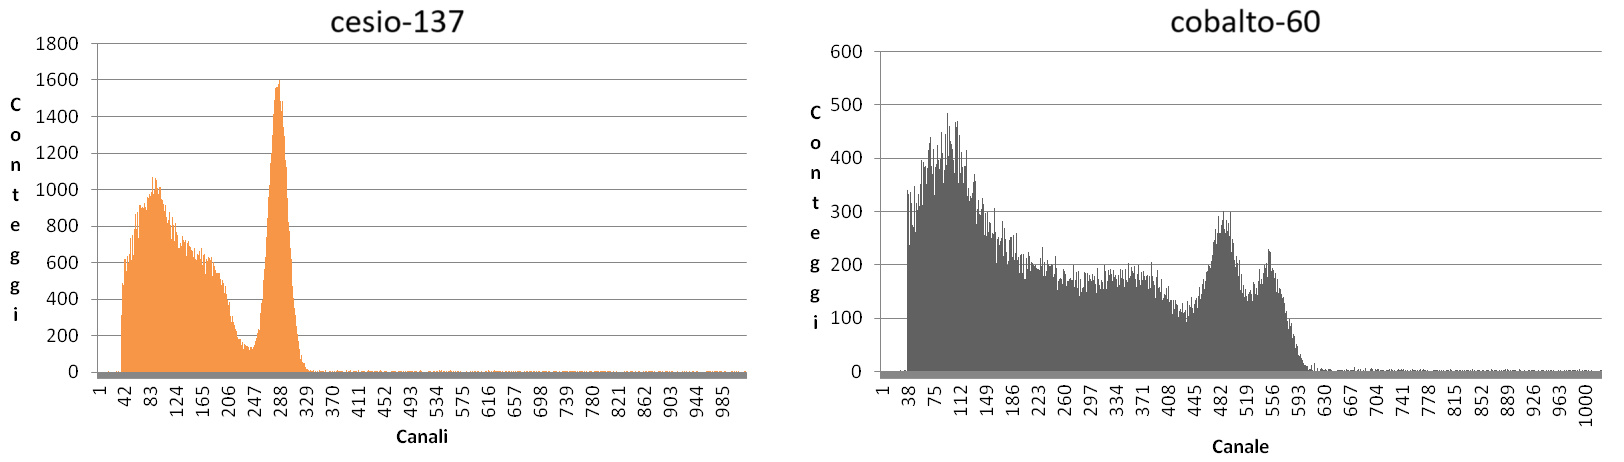
\includegraphics[width=\textwidth]{immagini/sorgenti_calibrazione.png}
\end{figure}
Adoperando queste due sorgenti avremo tre coppie di punti $\rm (canale, energia)$ relativi ai picchi fotoelettrici, per cui è possibile realizzare una procedura di best-fit per andare a individuare una retta di calibrazione come quella mostrata nella figura seguente:
\begin{figure}[H]
   \centering
   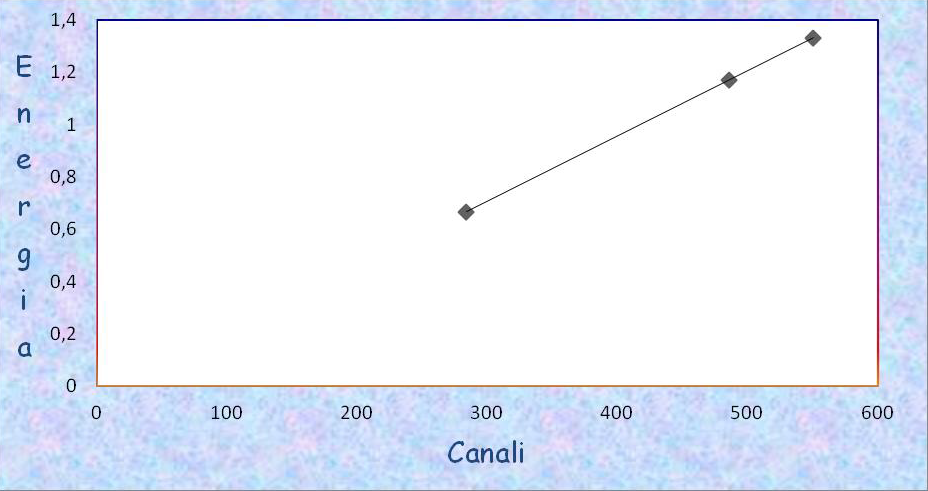
\includegraphics[width=0.6\textwidth]{immagini/retta_calibrazione_cesio_cobalto.png}
\end{figure}
Il motivo per cui la relazione che andiamo a cercare per ottenere la calibrazione è che nella maggior parte dei casi la relazione tra la grandezza misurata e il canale è lineare.

Attraverso questa retta di calibrazione è possibile fare qualsiasi tipo di associazione; ad esempio, se abbiamo una sorgente che emette $\gamma$ con una data energia, attraverso la retta sappiamo a quale canale aspettarci il picco fotoelettrico. Viceversa, se abbiamo una sorgente incognita e vogliamo capire di che isotopo si tratta, andiamo a vedere i picchi e in base alla posizione di questi rispetto ai canali possiamo, mediante la retta di calibrazione, conoscere le energie e quindi capire qual è l'isotopo.

Purtroppo non sempre la corrispondenza è lineare: a volte può essere lineare in una buona porzione dello spettro ma magari si presentano degli effetti di non linearità nelle regioni estreme (cioè nella regione a bassa ampiezza e in quella ad alta ampiezza), per cui è preferibile cercare di lavorare nella regione centrale dello spettro, dove la linearità è abbastanza assicurata.

\comment{\textbf{continua a 18:20 circa}

\begin{esempio}
   In figura possiamo vedere un esempio di spettro ottenuto con un rivelatore al silicio mediante una sorgente $\alpha$ con tre picchi di energia nota. Vediamo poi anche la corrispondente retta di calibrazione, ottenuta tramite best-fit.
   \begin{figure}[H]
      \centering
      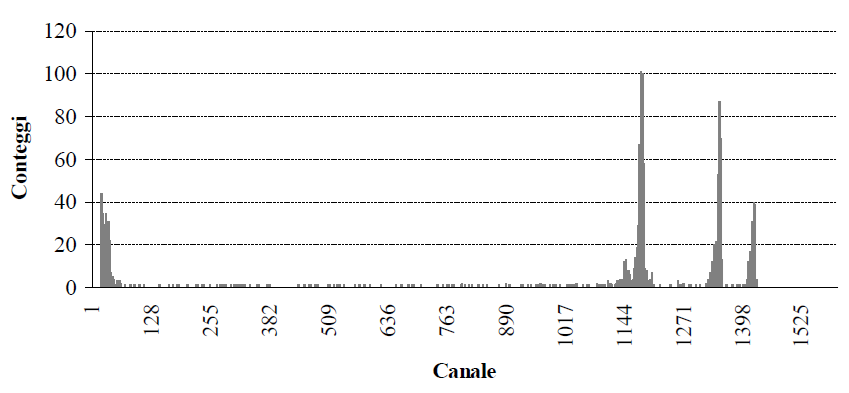
\includegraphics[width=0.7\textwidth]{immagini/esempio_calibrazione_spettro.png}
   \end{figure}
   \begin{figure}[H]
      \centering
      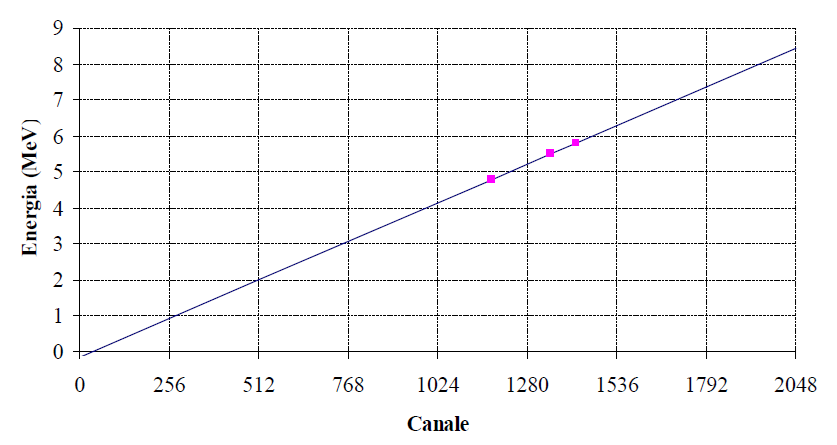
\includegraphics[width=0.7\textwidth]{immagini/esempio_calibrazione_retta.png}
   \end{figure}
\end{esempio}
questo è un altro spett, un esempio di direzione questa volta con un regolatore alzificio, quindi è stato solido per una rispura di particelle mescolare nella soggente alta la soggente alta non si potrà tirarsi sotto, dove le elettre, i titi di energia nota è anche in questo caso possibile realizzare una calibrazione vedete, ad esempio l'elettronica di di idealmente dovrebbe passare dal zero ma proprio per il tettino di linea di da, vedete che la gruva non interessa con le linee degli assi è una calibrazione che è oppurata, per esempio abbiamo anche le gesso agenti che non rispondono a energie più bassi o più alti, in modo a fare da andare a esplorare un modo di intera regione interessa tuttavia diciamo che già con questa soggentura si prendono delle ottime diverse 

\subsection{Risoluzione in energia}

la cosa che abbiamo notato è che tutti questi spettili che noi ci aspettiamo a essere molto energiati, ma non lo so, non mi è ovviso nel caso del suo programma, addirittura interventano diversi meccanismi, contribuono alla situazione, ma anche nel caso del suo gente alfa e le alfa sono sempre mon energetiche, i riantranno di se terminano dei ticchissi, come ci sarebbero aspettati da ticcicelle hanno esattamente tutta la stessa energia, arrivano i motivatori a depositare un tutta l'origeno di un un un mia spetterei effettivamente sentono lo stesso valore, quindi sempre lo stesso segnale di ukulele macchiazza, quello che invece notiamo è un allargamento del gico, a cosa è tutto questo è dovuto alla risoluzione energetica, cioè la capacità di un rivelatore di distinguere le rivezioni che depositano nel rivelatore energie simili, quindi immaginate di avere due rivezioni per rivezioni interne ovviamente sia la reazione del tuo magnetica che l'antica del del energie tra di loro molto simili, il rivelatore potrebbe non essere in grado di distinguere, di valutare che sono due energie effettivamente diverse, dipende da quanto vale la sua risoluzione di energia, come si valuta questo aspetto, questa è una carte istica dei rivelatori che misurano l'energia, l'esoluzione quasi restitucionata è l'inviato sul rivelatore delle rivezioni monoenergetiche, quindi se riprendiamo l'esemplice di prima, inviando delle particelle alfa e essere una sorgenza che sappiamo essere certamente monoenergetiche o utilizzando dei gamma anch'essimo energetici, e andando a valutare lo spetto in energia, quello che si osserva è non con una termini del grattuto, con con istogramma che si costruisce elastico elastico bin, per cui vediamo che gli eventi si subdividono su diversi bin, su diversi canali, a causa del proprio proprio questo effetto di risoluzione energia, quindi l'energia che le ripostruttiamo in alcuna certa precisione rispetto al monore vero e in conseguenza possiamo andare a valutare e la qualità e la riuscizione dell'energia andando ad osservare la lutezza di questo picco capite che il più essente il picco più il rivolatore sta lavorando bene in termini di misura dell'energia quindi la misura dell'energia è più riuscita e allora quello che si vado da è la posibilità della lutezza a metà lutezza del picco che in inglese viene pregiato con la sigla FWFM forno with ormai un massimo questa rappresenta la lutezza del picco alla metà della sua lutezza quindi andate a vedere il picco nel suo modemesso andate a vedere dove raggiungere il valore massimo considerate la metà della sua lutezza e andate a guardare che valore di acissa si raggiunge la metà del picco così i mestremi individeranno la lutezza del picco nella lutezza la risoluzione quindi verrà definita proprio come la lutezza del picco nella lutezza diviso il valore centrale del picco capite che state realizzando un rapporto tra due grandesi che sono entrate nell'energia, un intervallo di energia e energia centrale e con zero quindi quello che abbiamo è ovviamente una soluzione pura, un rovuro e che vuole veramente estrimere il percentuale sono un riferimento del percentuo l'antevolte è una buona prossimazione di questi vittimi che ottenete negli specchimi e quella d'Auxiana, quindi immaginare che il picco abbia una professione questa è una prossimazione che va molto bene, ha mai fatto dei casi e soprattutto nella zona centrale del picco, magari le potevi sono differine un po' da la sensazione d'Auxiana però certamente dalla parte centrale è una buona descrizione del picco e da questo rastro si può dimostrare che l'alvezamento è altezza la possiamo valutare conoscendo la devenzione standard della d'Auxiana infatti è legato attraverso un fattore motivativo vario 2,35 ok questo, dove dove torna utile? perché quando andrete a realizzare le denanzi dei dati di questi specchi quello che potrete avere uno specchio è il il quindi magari volete provare a realizzare un besfit con una professione d'Auxiana provare la migliora d'Auxiana che approssima questo picco e di questa dosi alla geramente tratti della prosciutola di besfit andate a determinare i paranti del picco che sono i centroidi da Algezza, quindi da devenzione standard e un fattore motivativo per rappresentare quindi la stessa del picco allora se riuscite a cambiare una prosciutola di besfit a valutare questi 30 metri il sigma vi può condare l'utile per lasciare la rapprezza metafrensia che altrimenti avreste dovuto calcolare con la prosciutola che vi ho scritto prima che non è oblidata la modalità però ho capito che può essere poco precisa per esempio quando il picco presenterà ovviamente delle tutte le strade di stile quindi anche a darini uguali esattamente l'ascisa e l'incorso sponenza della quale il picco ha avuto meccate la spoltenza magari non è facile a definire invece realizzare un besfit prosciutto che è una procedura che tiene conto anche 

delle prozionalismi stino che non si si fatto di distribuzione la procedura prosciutto quindi vi assumendo veramente questa slide uno degli effetti dell'eurobrità dei liberatori che miscolano l'energia è certamente la risoluzione energetica definita come la rapprezza metafrensia di sopille centroide banalmente qui vediamo confronto un liberatore con una risoluzione migliore fra una risoluzione del rosso o una risoluzione del dolore l'effetto è chiaramente elgente la valorezza del picco è maggiore nel caso ha avuto un'esoluzione del dolore e se non è edifici per i liberatori che vedremo il liberatore assilissimo che è stato solido 1\% in questo modo come risoluzione nel caso di 5-10\% anche nell'erivatore a gas la risoluzione non è particolarmente estima per il liberatore quindi in generale il liberatore assilissimo sono liberatori che hanno una buona risoluzione energetica forato la risoluzione di energia in realtà non è il sanem costante per un dato liberatore ma dipende dal valore di energia che state miscorando in generale più il delante dell'energia che si trate del liberatore migliore sarà la risoluzione di più colato della risoluzione per quale tipo? andiamo a distinguere di due casi diversi un primo caso è il caso in cui cui ramezione ha depositato parte della sua energia nel liberatore quindi non si è rifermata ma sufficientemente ha traversato il liberatore e ha depositato una parte della sua energia e allora in questo caso valvano tutte quelle considerazioni che hanno fatto questo tempo, questo stranio, questo fatto che possiamo calcolare l'energia media depositata, ma ma realtà da atticelle a fatticelle ci sono delle energetiche diverse perché intervenono diverse diverse sequenze di ippurti all'interno alcun punto di tenore all'interno del liberatore pensate a fatticelle cariche in un gas che producono ad esempio l'odignazione quindi non è detto che avendo prodotto sempre lo stesso numero di coppie, elettrone, rione questo numero può essere leggermente diverso allora, chiamiamo il gel gel numero di coppie, elettrone, rione quindi stiamo prendendo la considerazione questo caso specifico una particella carica che ionizza un gas in difere parte della sua energia questa energia viene utilizzata per la rione interna di gas gas se l'energia viene depositata e il blocco e l'energia media necessaria per creare una coppia elettrone e rione allora il numero di coppie è dato in media per questo rapporto e quindi suonoroppio ok? però abbiamo detto che non non pensato sempre lo stesso questo numero varierà possiamo stimare nella media e invece sono delle puntuazioni queste puntuazioni servono la distribuzione di passione e di qualsiasquela possiamo dire che la varianza, quindi sin prima quattro è pari al gel al numero di coppie che abbiamo considerato secondo questa polmona possiamo evadutare la risoluzione quindi la risoluzione, supponendo che la risoluzione sia di queste coppie sia gaustiana o possoniana va bene lo stesso che una possoniana verrà tutti i valori medi questa è postimata con una gaustiana vedete che l'avrei fatto per la mia postina quindi siamo nel limite della postimazione gaustiana però di base abbiamo una possoniana ok? quindi quindi applicare quella polmona che abbiamo visto prima cioè approfissimare la retretta metà terza come quel 35 SIGMA l'Asigma è la SIGMA di una gaustiana la SIGMA la posso esprimer come la resoluzione di di perché sto considerando una SIGMA e di conseguenza al numeratore nel calcolo della risoluzione vi troverò 2,35 RG diviso il segnale che è stato prodotto in Geli con la di coppie allora, la retretta andando a sostenire il Geli che era un po' esso doppio se ottiene la risoluzione che è 2,35 RG di 1,3 RG questo questo per dimostrarvi che la risoluzione dipende dall'energia depositata in particolare all'aumentare dell'energia la risoluzione diventa piccola quindi vedete come la risoluzione esittentemente legata a queste puntuazioni statissime ad esempio nel caso specifico della organizzazione alle puntuzioni che si presentano nel numero di coppie, elettore, ione che si generano quando viene depositata nella certa energia in questo primo caso dove avevamo presso un considerazione cioè quando la parte scelta deposita solo una parte della sua energia ma potrei avere dei rivelatori così spessi che la particelta della tensione si arresca all'interno del rivelatore quindi perde completamente l'energia che cosa cambia rispetto al rima che chiaramente l'energia di depositata sarà sempre la stessa mentre prima l'energia era solo una parte dell'energia di martenza e quindi l'energia versa tuttuale, cioè non delle legge varipizioni poi invece abbiamo un limite dell'energia depositata tra sempre e la stessa quindi è una risoluzione che questo non è un'energia utilizzabile allora si può dimostrare in questo caso la varianza non è data del J ma data del J per un fattore F che prende il nome di fattore di fanno che è un fattore caratteristico del materiale questo fattore di fanno è molto difficile da raccolare quindi il corso del tutto di materiale non è facile sapere qualcosa il fattore di fanno in Italia si può dire che la maggior parte dei rivelatori questo fattore è minore di 1 di che, ovviamente, incite sull'absoluzione perché ripacendo i passaggi della vista prima arriviamo a scovrire che la risoluzione dipende sempre da 1,12E però, vedete che sotto il semplice di l'ermice compare il fattore F quindi dice fè minore di 1 perché la risoluzione è influenzata da questo fattore oltre a tutti questi scossi che abbiamo fatto sulla risoluzione che sono più legate al rivelatore posso intermedire anche altri fattori che peggiorano la risoluzione energia 

in qualcosa disegno dell'electronica scusciata al rivelatore potrebbe influenzare dettagliamente quindi aggiungere tutti i due e ponde di incertezza e quindi peggioramento nella risoluzione energia più altri e ventoni fattori che dipendono dal sistema caratteristico che è stato utilizzato ora se queste sono tutte fonti dipendenti come normalmente è, è perché magari il rivelatore è anche scollegato dall'electronica quindi non sono dei fattori che sono dipendenti di uno dall'altro, sono dei fattori tutti dipendenti in caso caso allora, vedete che il ciascun contenuto si possono fare un'acquadratura per andare a valutare la risoluzione energia di la confezione quindi quando avevo un sistema e di potere si conoscere la risoluzione del rivelatore ma bisogna sempre ricordare che questo è un punto diversico per il suo suo quindi rivelatore in tema ora beh, se c'è un ponte in cui direi per la rivelatura o per l'altro Vediamo alcuni esempi rispettivi per cui è piaciuto per capire la risoluzione, ad ad qui abbiamo una misura di energia e di particele ampia che sono valutte da una reazione per aver scritto qui il video-set per il suo video-set che produce alpha e miglior stena i quindi sono particelle alpha valutte da una reazione che vedono rispurate come un rivelatore di silicio La risoluzione ad esempio di questo tipo che vedete, di galvanare non combinazione è 150 k, in termini della testa su 10.9 m, che è la posizione del centroide se vi fate conto questo è 1, che è quella 4 per 100 in termini di di che è una posizione posizione posizione posizione posizione posizione silicio anche se misurate a alpha e vado a a a sorgente con la fredda di un uoica paratoria con le cose simili ad esempio questo uno spettro è acquisito con una sorgente di amperista di alpha che lo utilizziamo da collaborio vedete questi per picchi un picchetto satelite si può realizzare un desperate di ossiano si può valutare la sinima della posizione e favore la questa risoluzione e vedete che questo amore si torna con valori del 1.100 se volessimo avere risoluzioni migliori del 1.100 è necessario riporre ad alta strumentazione in particolare è per te di uditare dei sistemi basati su spettro mentre i manienici i sistemi che adobrano dei manienici per pulvare le particelle iniziate verso dei rilettori in base alla traiettoria servita della vanticella si conosce assentemente l'energia e dove in questo caso si può arrivare a risoluzioni molto più spinte ad esempio guardate questo spettro guardate questo picco che semplicemente ha un picco a 5,7 m con una risoluzione di 2,5 k quindi 0,2 ,3,4 300, quindi molto di sotto del 1.100 che abbiamo visto in questa verità immaginate se avessimo avuto l'1 .100 quali sarebbe stata la consaguenza l'1 .100, un picco lici il K6M se vi fa il conto colispa un K60K allora se fate 6M-60K e 6M-60K capite che sono sostenete tutti questi picchi che vedete qui per il nostro tutto quindi questi ultimi 4 picchi sostanzialmente per reglero un fusi in uno collato perché la risoluzione d'energia non permetterebbe di distinguere un picco dall'altro cioè in ultimo ciclo sarebbero così laghi che a melebra sono forse in uno picco e non riuscireste per risoluzione quindi l'effetto della risoluzione è di permettere di distinguere dei picchi in energia che sono molto riuscili per loro almeno anche il rischio a che si mamma il suo suo in un collato è un esempio che l'avevamo già visto nel caso dello spetto del K60K vedete che qui abbiamo dei picchi molto riuscili per loro che sono parzialmente sottocotti ancora riusciamo a distinguere immaginare se la risoluzione fosse stata un po' peggiore questi picchi sarebbero così un picco e non avevano più distinto i due valori di energia con cui vennero mesi trammati e e e la la di un K60K quindi quando si vuole trattolare una misura, non abbiamo riusciuto ovviamente a questa catta di istituzione resistenta alla risoluzione energia per il risoluzione di resistenere il riuscito riuscito trattolare le risoluzioni che si intende a realizzare adesso andiamo a qual qual una traspetto della mia regla di ritorno sono domande, comunque, che non non visto la risoluzione sei una risoluzione percentuale del, per esempio, lei ha fatto il rapporto tra la semiampiezza e l'energia che ha associato il risoluzione di resistenere resistenere poi ho fatto, per esempio, 2.5 e 5 è una risoluzione del 8.5\% ho la stessa risoluzione però per 0.5 e e però il picco mi si allarga decisamente quando ho l'energia ovviamente dipende del valore di energia che stai ispirando, quindi non sono... che più non è in testa come risoluzione come siamo abituati noi, che più ha presso il picco più non ha risoluto, è più una cosa di rapporto esatto, e da quali che sono poi il collega ha chiesto in dettaglio la denunzione di risoluzione perché lui ha detto, non è sottile che la risoluzione che trovano a partare è la largherza del picco, ma ma realtà non conto solo la largherza conto anche il valore di energia questo insumiamo la largherza sì, è vero, è vero, dire 50K su un membro o 50K su 10M e adesso ovviamente dipende la largherza di energia, quindi si è una largherza di tenita al valore risparato mi ritroverete a definire invece una passione di un'automo una largherza in assurdo quando si va ad esattre a migliorare la risoluzione temporale di un sistema allora io sento possa parlare proprio di largherza del piccolo in un 2 secondi senza aver affrontato il valore di energia come ti dipende da quello che si vuole se lo spettacolo poto metterlo digitale che avrete ad elaborare in lavoratorio abbiamo una spettacolo di radiazione luminosa quindi vedete c'è scuola nuovezza d'onda che invenzità viene messa da una solleggente allora in qualsiasi avrete ad esempio delle sorgenti idealmente ronormatiche come ad esempio un delto colorato un delto rosso vedete la luce rossa, le spettate durante la solleggione potometro di imparare ad esattamente una spettacolo di nuovezza d'onda di grima niente rosso invece non è così i led sono monocromatici ma fino a un certo punto vedete che in realtà sono compresa ad esempio un ex d'onde del caramcione quindi abbiamo un algello o un altro ex d'onde allora in qualsiasi avrete una solta risoluzione questa sorgente luminosa a più senza quella considerare in assoluto non raccontare il valore di un ex d'onda inserzionale è 

valore in bar di planarcazza quindi dire che in l'end emettere la sorgente con sfondo un piccolo con una valorezza di una decina di danone di l'ultimo con un senso da ventile per fare un conto quindi poi le abbiamo dicono se volete corretto in questo caso la risoluzione dell'energia si consiglia a qualcuna potenza quindi in qualsiasi anzate l'energia ha costruito quando non si cira altre domande se non ce ne sono andiamo a guardare un altro aspetto dei lavori dell'efficienza l'efficienza di un liberatore questo è particolarmente importante nel caso delle vetture di fatticelle neon trepone di ottenuti neotroni di cui non abbiamo parlato non abbiamo sempre detto che è qualcosa di abbastanza onioso possiamo dire che sono fatticelle che interagiscono con meccanismi diversi a quali che abbiamo visto delle patticelle neon trepone hanno inefficienze novevole di liberazione quindi è molto importante sapere le efficienze di liberazione però il concetto di efficienza in termini di liberatore vale per qualsiasi tipologia di liberatore in fatto non è detto che tutte le radiezioni delle patticelle che incitano per liberatore sono interagiti di impurre con un senale insurabile pensate a base di un gramo i gammati o arrivare sul liberatore, ma oltre a venerdì interagire attraverso una delle meccanistiche che hanno un disco che pronunciere in questo caso il gammato di le persone viene insurrato quindi è arrivato sul liberatore idealmente avrei dovuto rispurarlo ma non lo ho ho oppure pensate a una macicenda calica che per fatto il motivo deposita poche energi al liberatore e produce poche un segno di bassa ampiezza e la roba del segnale viene con un suo ponte di rumore e non viene risurato quindi ci sono dei passi in cui il liberatore è un essere inefficente allora proviamo a valutare a condividare con una grandezza questa efficienza che si dice è efficienza in trince da quanto dipende proprio dal liberatore delle meccanismi di interazione della radiezione con il liberatore e allora le efficenze in trince con il liberatore che definita come il lungo di patticere che vedono liberate e che produce un segnale che viene in qualche modo acquistito rispetto al lungo di patticere che incidono di cui il liberatore ok, quindi una demizia è molto semplice anche se semplice non è facile valutarla perché le efficenze in trince dipende da quanti aspetti dipende dal tipo di patticella e quindi quindi quindi quindi quindi ad esempio potresto avere un liberatore molto efficente per la misura del grama ma un po' efficiente per la rivelazione di un pizzo in le cariche o un pizzo l'essa pensate a un liberatore al patticell generalmente li ha lavorato per le patticelle cariche e in un patticell di pizzo in patticell difficilmente va a misurare un grama che chi chiama il grama che si vedecevo con la valeria di Murioccio e quindi ha una efficienza che dipende fortemente dal tipo di radiezione che sta incilendo sul liberatore dipende dall'energia della patticella perché la terza lona dell'energia intervengono dei meccanisti di rivelazione di pazzi dipende dal tipo di liberatore chiaramente, ma anche dal volume del liberatore quindi quanto prenderà un liberatore se per causa della radiezione può fuoroscire, può non essere misurata proprio a stato dell'energia di un liberatore quindi ci sono tanti aspetti che rendono la valutazione di questa efficienza inizia a un compito non semplicissimo che spesso viene fatto in patti con dei codici in simulazione professionali che devono conto un po' i meccanismi di interazione che costano ottenere e permettono anche di modellizzare in maniera un'autoria districa che rivela il corso corso sta dovendo un'altra vattoria da considerare oltre ad efficienza inizia è la cosiddetta accentanza geometrica o efficienza geometrica questo è un concetto diverso che lo abbiamo usato prima prima ci siamo senti un problema di quello che succede, una patti scelta che arriva a colpire di rivelatore a minuse colpisce di rivelatore nel senso proprio di tradittoria di arriva a incidere il rivelatore e viene rivelato meno adesso invece ci muoiamo proprio il problema di capire se una patti scelta è messa da un personaggio ad esempio arriva a colpire o meno il rivelatore indipendentemente dal fatto che forna una volta intercettata il rivelatore si congurono semplicemente ok, così sono due concetti un po' diversi infatti l'efficienza geometrica o accentanza geometrica e definita come uso di patti scelte incidenti col rivelatore sul numero di patti scelte e messe da una sorgenza facciamo un esempio banale ma se io avrei una sorgenza come mi segno, non mi fai un pittore di forme da questa sorgenza che non è messa delle patti scelte non lo specifichiamo non è una una scelta, ma è una importanza e vengono messe in maniera sottova quindi con la stessa propria digitazione di tre direzioni dello spazio capire che se la rapicella viene messa in questa direzione quindi nella direzione opposta il rivelatore non potrà mai impirare il rivelatore sono tanto quelle che intercettano l'angolo solido sotto il rivelatore continuando il rivelatore questo caso il rivelatore è schematizzato con questo valore del rivelo di su 20S che si trova a una distanza r dalla spazio e allora se volete valutare l'efficienza geometrica capite che tutto si riusce a avvucare lo geometrico che dipende dalla sorgenza e dalla rivelatore quindi da un po' di schifo con la mente geometrica quindi se siete bravi in una geometrica possiamo valutare l'efficienza geometrica perché questa niente è è come che rafforza l'angolo solido sotto il rivelatore e l'efficienza geometrica quindi da vinto che al sempre spesso si fa da un fisico di rivelatori in quattro pd, da che cosa si intende si intende da rivelatori che vanno a circondare per intero la sorgenza da cui costruono queste prodotte delle particele ad esempio l'HGC dove avevano delle commissioni tra fasci di punto di interozione che è totalmente circondato dai rivelatori che sono normalmente di forma cinica per andare a misurare tutto ciò che emerge da valutazione però nella maggior parte dei casi il rivelatore ha una tua dimensione e posso lasciare la distanza dalla sorgenza e quindi bisogna provare a decorare questa efficienza geometrica allora se ne andiamo a fare una approssimazione immaginiamo che la distanza tra sorgenze e rivelatore sia molto più grande delle dimensioni del rivelatore allora possiamo immaginare di approssimare la superficie del rivelatore con una superficie di una barocca sperida che ha un avvicinato proprio della distanza sorgenze rivelatore e allora in questo caso il canto è facile perché l'anno solido per una potenziale rivelata sperica a una distanza ebre lo possiamo rascrire come essere su un r4 diviso 4t, da vita, per la tua accentanza geolentica da vita e e questo per il resto per 0, 1, 0 vuol dire che l'anno solido è 13,0 1 vuol dire che l'anno solido è 4t, se l'esempio di rivelatori può può tutte le pappuccelle che abbiamo remesi nella parte di destra sveglia sottentemente allora avreste una mozione di anzolio pari a un pidega e un efficienza entroletrica pare di un peroscicchio, qualsiasi quanto ha l'eccepto tutto ciò che viene messo da l'altra mata sinistra che l'anno migliorato tuttavia non è sempre così semplice calcolare le efficenze geometri, la prima cosa è è prossima azione ma immaginate le rivelatori che hanno adesionato alla solide non possiamo più fare con la prossima azione per non assolutività e allora finché ci manteniamo con geometrie semplici esistono delle pocole analitiche ad esempio si può dimostrare che in caso in cui il rivelatore ha la buona lunga cilindro che la sono già in tutti i formi è possibile calcolare l'angolo solido sul tezio della rivelatore ancora verso questa forma doverle la distanza da sorgenza e rivelatore e a eurice cilindro quindi avrete una forma che rivela la sinistra calcolare l'angolo solido e il conseguenza di scienza geometrica ma già, banalmente se conflichiamo un po' di più il problema e immaginiamo di avere una sorgenza in stessa quindi non più più di forma ma una sorgenza che magari ha un bischetto con una sua dimensione sinica quindi in realtà la emissione delle praticelle può ottenere da qualsiasi punto di questa sorgenza c'è un problema più contesto che si risolve attraverso l'internazione di funzione di Bessel attraverso dei medi numerici c'è una soluzione approssimata se volete del prodotto però per l'ingredio deve diventare un problema analitico contesto forse si fa in questi passi si riesce adottare delle tecniche di sinurazione a non rivelarlo e quindi quello che faremo quando conteremo le lezioni in un punto quindi faremo delle simulazioni per calcolare l'efficienza geometrica di un rigolatore che è un un di durazioni per vedere che subtendono dei risultati in apporto con i valori di resimulazione non vuol dire qualcosa di postimato ma se ci si rivolta un mondo preciso anche di farleare alcune carte risiglie dei valori a questo punto descriviti questi due specchi 

dell'efficienza l'efficienza interna e geometrica possiamo valutare l'efficienza possessiva del rigolatore perché capite che a un fine il fatto che una macchetta venga effettivamente rivelata dipende dai grandi rispecti dipende da un rischio geometrico dal fatto che è una macchetta segmana traiettoria che va a intercettare il rigolatore e poi dipende dal fatto che è una macchetta del rigolatore che indiomente segnare il prodotto sia sufficientemente elevato da poter essere intratto quindi, l'efficienza possessiva è dalla semplicemente del prodotto tra efficienza interinsega ed efficienza geometrica se andate a prendere le dimensioni che vi ho dato prima l'efficienza interinsega è il numero di baticelle rivelate sul numero di baticelle tucidenti l'efficienza geometrica è il numero di baticelle incidenti sul numero di baticelle elessida la macchetta sostanzialmente diciamo a sincronificazione quindi il numero di baticelle incidenti si certifica e poi non le rimane che l'efficienza complessiva del rigolatore è il numero di baticelle rivelate sul numero di baticelle elessida quindi tiene in conto gli entranti di rispetti quindi il gamine è un totalmente più piccolo di tanti fattori conoscendo l'efficienza possessiva si possono correggere gli attività di valutare le quantità originali cosa voglio dire con questa tasse supponete di avere una trangente in lavoratorio e volete adattare l'attività di l'efficienza quindi quando le baticelle entrano a essere al secondo allora abbiamo un mostro del rivelatore che non è la forma di un cilindro come quello che vediamo qui l'ho posizionato a una certa distanza che è una talda di fredda l'altro l'altro l'altro l'altro l'altro quindi l'ho posizionato in una distanza di generevole che è in tanto da contare queste quanticelle arrivano al secondo ma questo numero che è data misurare chiaramente non corrisponde con l'artigiatura della sua gente perché di tutte le particelle messe della sua gente voi le state misurando solo una opzione quelle che entrano nel lavoro solido su un teso del rivelatore e più di quelle che entrano nel rivelatore è che non è è è tutte viano luogo l'ansigliare e quindi vennero a rivelare quindi se io conosco tutta mia l'efficienza possessiva posso conoscere l'attività andando a correggere la frequenza di conteggio proteggo sperimentemente dividendo la terra di esplicenza che è da questo caso posso risalire nell'attività della mia sua gente è chiaro che però devo conoscere l'efficienza ora se l'efficienza interinse che ha una cosa assicuata che può essere un'altra c'è se suppone che sia 1\% 100\% se l'efficienza interinse che ha una cosa che possiamo affrontare una volta che vi dà l'emozio di strumenti per la risolta o per le novità che sembri che la poter utilizzare per le forme della mia amisto prima oppure si riporve alimento di modellarlo per la lucezza e la efficienza di l'unicefine e quindi la sviluppo di una terra di esplicienza con l'automotore ci sono domande se l'efficienza è chiaro? anche da fuori se ci sono domande non non non non è una una è è vita allora andiamo avanti e andiamo a analizzare un altro aspetto davanti a queste interessate a conoscere il tempo di risposta di un riferatore perché questo può formire delle indicazioni in modo modo segnare che viene formito da un riferatore e poi la riconosce sul tempo di arrivo della particella per la riuscione e quindi in generale è importante anche sapere con la precisione con cui viene formito questo stando di arrivo nella particella quindi la cosiddetta è la risoluzione ancora del sistema quindi qui la quantità che stiamo andando a misurare da netto di energia del si è in tempo di arrivo questa informazione può essere formita anche a stalla una certa precisione anche in questo caso la risoluzione temporale dipende da tanti fattori dal tipo di riferatore dal metodo, del modo di conoscenza del riferatore le dimensioni del riferatore che influenzano magari la accolta del segnale e l'elibronica associata alla riferazione del segnale perché è importante conoscere la risoluzione temporale di sempre potrebbe essere intottante ma non si otterrano delle misure di tempo di loro time flight che spesso troverebbe abbagliato alla sinna tozzo infatti per andare vedremo da andare a identificare le particelle, le toniche che che aprire il tipo di particella sta passando potrebbe conviene andare a misurare il tempo di loro cioè il tempo che tiene la particella per porre la base di loro per passare da un punto dello spazio per andare dentro dello spazio come si fa questa 

risola prendo due riferatori in due ristrioni del decise e andando a misurare il passato di una particella che attraverse il tramite quindi che conoscendo il tempo di arrivo in risoluzione temporale che si trasponde di arrivo il tempo di cosa la differenza per i passi di due tempi e la risoluzione temporale che è veramente pressiva questa risoluzione trasponde della somma in qualitatura delle risoluzioni temporali dei riferatori quindi il tipo di riferatori rappresenta le risoluzioni di una capacità di andare a misurare il tempo di arrivo in una particella che capite che stiamo parlando comunque sempre di tempi molto brevi nella maggior parte dei casi dei misuriti, un po' di volo spesso poi sponde una misura dei tempi verdissimi immaginando le verde della particella se stanno movendo la velocità prossima a colore della luce in 30 cm nella nostra condola quindi, per per se abbiamo posizionato i riferatori a un metro di vista non state a vedere quello che vi è aspettato sono tempi dei giorni di tre e una o due secondi di di la vostra risoluzione temporale deve essere più piccola di questi valori a primelli a 600 km per per è la risoluzione quindi bisogna anche saper scegliere bene che i riferatori la dobbiamo fare in passanti al giorno di via in questo momento per implementare ora, tipicamente i riferatori a gas sono dei riferatori lenticoli con una strada di lenti e di conseguenza le riferatori a gas sono difficili perché con un riferatore a gas tranne con eccezione vengono lavorati per l'artispole di tempo altri tipi di riferatori a gas sono sensibili proprio per ovviare questo problema e noi vediamo qualche eserio per arrivare anche al riferatore al riferatore di centinaio di questi valori in generale i riferatori in passanti di scinsatori vediamo i riferatori a 9\% di i riferatori per l'orche a 10 secondi quindi ad esempio che ho fatto vedere prima, vorrebbe essere realizzata con due scinti del vettore, per che forniscono dei segnali abbastanza veloci. Un ultimo aspetto che vediamo per il vettore riguarda il cosiddetto tempo l'8. Infatti, il ciascun sistema di rivolazione ha visto di un certo tempo per processare il segnale e durante questo tempo se arriva un secondo evento, questo secondo evento non viene rivelato, quindi viene perso. Come arrivano gli eventi nel tempo? Se eseguano un'instituzione di possono, non lo sapevo se se lo abbiamo fatto, non lo sapevo se lo non lo non E andate a vedere la differenza di tempo tra un evento e successivo. Allora, questa differenza di tempo si distribuisce secondo una distruttuzione esponenziale deficente. Quindi è molto probabile che la differenza di tempo sia piccola tra due rendi. Quindi, indipendentemente dal tempo morto, c'è una probabilità non di un da che si possa verificare un secondo evento durante la finestra del tempo morto. Quindi è qualcosa che bisogna conoscere e valutare. In particolare, una volta che si conosce il secondo morto del sistema, si deve cercare di andare a misurare qual fenomeni che hanno una frequenza di contento ovviamente compatibile con il tempo morto del sistema. Quindi, in un'una delle frequenze di contenti elevate che comporta la vera vita di tanti eventi. Quindi, in base al tempo morto, si stabilisceTake, sostanzialmente, il limite della frequenza di contento insurabile. E' chiaramente ideale avere una risposta del locio e la pace dei liberatori. Ci sono due nodelli per descrivere il comportamento di un liberatore dei contenuti del tempo morto. Abbiamo i considerati liberatori non parali risparalizzabili, che sono dei liberatori in cui un evento che accade durante il tempo morto con influenza, ulteriormente, il comportamento dei liberatori. Quindi, ad esempio, guardate questo schema. Immaginate che questo sia un primo evento che arriva, queste venti chiaramente produce qualcosa nel rivelatore, il l'elettronica, il processo essenziale, tutto ciò richiede un certo tempo prima di si rilistina, si rilistiranno le condizioni per una nuova rilalazione. 

Sumpendete che questa è una severuale e che questo qua sotto sia l'intervallo all'etato a tempo morto, che è parte chiaramente quello arrivo del primo evento. Quindi, in tutta questa finestra, se arriva un secondo evento, un secondo evento viene verso. Ad esempio, secondo me, arriva qui, viene verso, ma non è influenzata la finestra del tempo morto, quindi non va estendente, una volta complettata questa finestra, il rivelatore sarà pronto per la rivelzione e se arriva un nuovo evento sarà pronto un misurato. Il cioresso, un rivelatore paralizzato, i venti perci comportano in una maniera differente, lo vogliamo direttamente nello schema, vedete qui il pericolo al primo evento e partita la prima finestra di tempo morto, arriva un secondo evento, sempre nella prima finestra del tempo morto e questo massiche il tempo morto è esteso. E così via se ne dovessero arrivare altri. Quindi, complessivamente, la finestra del tempo morto si estende, e continuano ad arrivare i venti. E i rivelatori sono fatte nere a una di queste due categorie. Come facciamo a valutare quale è l'effetto del tempo morto in un sistema sul momento di rispontesi? Non glielo che abbiamo misurato in un certo numero di contagi, sappiamo che questo sistema ha un suo tempo morto, come fa a ciascè, se quello che sto misurando vuole rispondere veramente alla frequenza di contagi, ovvero, o se lo perso degli eventi. Allora, supponiamo che il R mis sia il rate di la frequenza di contagi misurato, R vero e Tau il tempo morto. Allora, si può dimostrare che il caso di un rivelatore non paradidabile è valido a questa forma, cioè la frequenza di contagi opera è legata alla frequenza di contagi misurata attraverso questa relazione doveva valare il tempo morto. Quindi se io non ho scritto il tempo morto e il misurato, una certa frequenza di contagi, posso andare a calcolare tra questa formula il rate vero. Chiaramente più di l'anno di tempo morto, il rivelato vero e il rate misurato, si tritescono, è chiaro questo. Nel caso di un rivelatore paradidabile, purtroppo, la relazione è un po' più contessa, la vedete scritta qui. Quindi se non è una relazione per un sito di grandese, ma è una relazione che è di essere risolta attraverso dei metodi teratini. Tuttavia, nel caso in cui la frequenza di contagi è passata, per entrambi i casi, si può arrivare all'attroximazione, che è scritta qua sotto, è in parte saltata, però non riuscire a berella, il rate misurato corrisponde al rate vero per uno meno il rate vero, tau? Quindi attraverso questa relazione posso risalire il rate vero. Ad esempio, utilizzerete un sistema per rispondere le pratici delle alfa, le dei gamma, un sistema in posizione dati dove il vero ha formito il rate, più che il rate vero è il vero ha formito il tempo di misura reale e quello è il tippo, quindi sanno più tempi diversi, uno è il tempo che è trasposso, il tempo che possiamo misurare l'altro è il tempo in cui il sistema è stato realmente tippo e quindi, per questo, possiamo valutare il tempo molto. Ok? Quindi, se conoscete questa informazione e andate a misurare la frequenza di contagi, possiamo risalire alla frequenza di contagi. Quindi, se non se non se non l'impasto di corretto, possiamo, in modo di eventuali perdere dovute a un sistema di acquisizione. Vediamo alcuni esempi, alcuni calcoli realizzati con un po' di x-ray, per capire qual è l'effetto del tempo molto. Fumbo, vedete, di avere un tempo molto, di 10 minuti, qui ci sono gli assiccenari immaginate di avere delle sorgenti che pronuncono dei rate più e più crescenti, quindi da 10 Hz fino a 5.000 Hz, questo è quello che viene invece misurato a causa di questo tempo morto. Allora, vedete che, nel caso di rate passi, un tempo molto di 10 microsecondi praticamente non fa perdere quasi nulla, perché 10 Hz, vuol dire, 10 particelle nel secondo, una o di 0,1 sec. Avere un tempo morto, 10 microsecondi non fa quasi nulla, perché qual è la probabilità che di quei 20, per esempio, i individui ricarano in 10 microsecondi, molto bassa da dove i media sono separati da 0,1 sec. Ok? E quindi le perdite, in questo caso, sono veramente i risoli, 0,01\% Capite che aumentando il rate, questo effetto è il rate più consistente. Per esempio, guardiamo l'ultima linea, questa 5.000 Hz. Vedete che in questo caso abbiamo una perdita del 5\% cioè 10,5 sec. di tempo molto molto morta già di 5\% di perdita per i periodi di pereria. La cosa bella, se è il tempo molto più grande, ovviamente, vedete appunto che si può arrivare anche a perdere quasi il lame tali degli individui a causa di questo punto. Quindi, per dentro, al solito, da una frequenza di potenza, questa è la ora, quando è il tempo molto di sistema. In generale, se è importante in due grafico, il rate derero, la frequenza di potenza di potenza di vera, e la frequenza di potenza di uno miscurata, idealmente, dovresto avere una retta che è la risentrisha, che dovrebbe lo corrispondere, se si stiamo a costruzione ideale. In realtà, ci sono delle perdite per il tempo molto, e vedete che queste perdite hanno, dipendono, ovviamente, il tempo è sempre più consistente di quanto è la tua retta, ma soprattutto dipende anche dal mondo di funzionamento del liberatore, se è paralizzabile o non paralizzabile come l'ho visto prima. E guardate, nel caso non paralizzabile hanno inizie poi stessi, ovviamente, si sia una merita, ma è una perdita abbastanza limitata. Nel caso del paralizzabile, vedete che conto, il risalto è stato così paralizzato, perché non hanno un tempo molto che è stesso, che arrivano, che via sempre, fatticelle all'interno per la stessa mia stella interna, e quindi il rivaratore, appendamente, può prendere quasi le fatticelle che arrivano. Questi sono altri tempi, nel caso di rivaratore non paralizzabile, i termini, per il risalto di interna, hanno un tempo un vedete che è chiaramente una mano, dove ha un tempo molto, e in questo direttore, è sempre più evidente, perché anzica, è una disentrice mano, questa è una stessa, il tecnica che il re il ritorato è più difficile del re, e non è sempre più evidente. L'ultimo slide, su questo, non è una titanza, riguarda, come possiamo istimare il tempo molto, a volte ce l'è dato direttamente, dal ritorato, per un sistema di apposizione completo, e che viene formato il tempo molto, ma se non abbiamo disposizione questa informazione, come si può disvolare, si può fare sperimentalmente, in particolare, esistono diverse dettiche, una tecnica molto doverata, è un considerato metodo delle persone detti, che consiste nell'andare a utilizzare un rivaratore 

e a posizionare due posizioni disseltate e dei sorprendenti. E allora si fa una prima misura, solamente con una delle sorgenti, e si fa un misurare, cosi detto rate 1, poi si fa una misura con l'altra sorgente, e si misura il rate 1, e poi si fa una misura con entrambe le sorgenti, e allora direttamente, cosa mi aspetto, se il tempo molto, osserva veramente riscurabile, il rate misurato deve essere la soltà, ovviamente dei pure rate, R1 e R2, e quindi il quindi il quindi il qualcosa di meno, questa divena di venerata di influenze del tempo molto, e si può utilizzare questa formula, che è l'edetretto, solamente questi tre rei che abbiamo dettito, che è veramente di calcolare il tempo molto, questo è un metodo che è, diciamo, abbastanza semplice da lavorare, qual è la difficoltà, che comunque sia, ed è anche alla statistica che hanno da usurare, quindi è tanto preciso, quanto perlù dalla costura che è perquale, perché la situazione statistica, ovviamente, diventa la semprella in un modo di rilassaristica. Dipende della capacità degli osprei rettatori, posizionare le sorgenti, nel stesso punto, perché la vita bisogna fare le tre misure, una con una sola sorgente, una con una altra sorgente, e una con una altra, quindi dovete spostare le sorgenti, che posizionare esattamente una sorgente, non se sponge un uniero. Quindi, comunque, questi, rimano a precisioni, che vanno il tempo molto, ma ci sono le loro, e in qualche per cento. Ci sono tecniche alternative che fanno uso di generale gli impulsi, però adesso non diciamo nient'altro, però di conto. Voglio solo dire che ci sono anche delle rettini che hanno un po' un preciso aspetto a questo metodo che abbiamo visto adesso. Ci sono domande, che dopo molto? Ci sono Ci sono Ci sono Si è dopo due volte. Ora facciamo la vostra. Ora facciamo una cosa che ci rivediamo nel lenti. Ok? Adesso, noi siamo alcune tante tine di rettatori che ripartono ovviamente il fatto che il liberatore mostra un tempo di curare l'energia, che è una tante tente di rivolverla, vero? In realtà, secondo te la tipologia libera, è possibile avere accesso alla terremotione che le retticelle incidono. Ad esempio, oltre all'energia, si poter di insurrare un po' il che, in un modo, ad altra energia, che ha un'importazione sull'energia della parte di scelta, perché la via, quando si stanno lavorando, volerà l'energia, cioè l'energia molto stridigrante nella massa rivolverla, la parte della cella, l'energia di impulso, c'è uno inizio che la sostanzione intera per il volo di energia. Carica, massa, tempo di activo, quindi, a servo al sistema che è stato portato, poter avere accesso diverse informazioni. In generale, per aver accesso tutte le informazioni, dovete avere esposizione impossibile a un unico rivolatore del suo misto. In realtà, se stiamo siano grandi sistemi di rivoluzione, anche perché abbiamo fatto un sapore diversi, possibili magari diversi sotto i rivolatori che scuttano tecnologiche diverse. Quindi, adesso faremo una ricissima introduzione a un rivolatore che ha uscito da tanti sotto i rivolatori, come viene nel caso di tutte le rivoluzioni di la pubblicare e la difficilitare. Ad esempio, quando si vanno a insulare dei regimi di energia molto elevati e, ad esempio, si vanno a studiare le condizioni tra fasci di particelle a energia molto elevata e quello che succede è che la passiamo di visioni per connessi di attissime particene. E di conseguenza, i rivolatori che sono in lavorare sono rivolatori estremamente conversi, non solo dovono essere rivolati per andare a misurare tutte le particelle messe dal punto di interazione, e avrebbe il caso di necessario rivolto in geometria, fatto di greca, che è normalmente piena assicurata con queste geometrie cilindri che accorgono il punto di interazione più degli end-up, cioè dei rivolatori che vanno a fare la rivolta in gida tappo ad essere in termà. Quindi non solo un'efficienza al possibile prossimo 100\% ma anche delle tecnologie che permettono di capire le diverse tipologie di particelle che sono state prodotte per andare a studiare diversi segnali di tifo. Quindi, come questi sistemi di rivolazione effettuano queste operazioni e a un punto abbastanza confesso, devono sapere ripostruire le tracce delle particelle, quindi devono essere alcuni dei rivolatori di tracciamento cioè i gravi che deve andare a visualizzare in qualche modo il passaggio delle particelle, e andare a tracciare quindi delle linee, che in questo caso delle curve che presentano un capo manierico con una delle linee che rappresentano il percorso seguito da diverse particelle. Devono essere in grado di identificare di sapere di tico di particella la massa della particella che è stata misurata oppure, essere in grado di sempre di percorare poto mangiare anche di alta energia. Ora, uno dei conti che punte il misurare l'energia, e già ne aveva anticipato che questo è un aspetto importante soprattutto quando si vanno a misurare di sempre elettroni o fotoni di alte energia anche in quei casi se ne ricordate, si produrò degli sciami elettromagnetici per misurare l'energia dell'amore dell'elettrone di partenza è necessario di percorare dei rivolatori in grado di contenere eventuali sciami che si sgruffano. E questi rivolatori che vanno a misurare l'energia totale di una particella, di una latenzione sono attività unimetriando con uno scopo di andare a misurare l'energia totale di la particella. Possono essere i calorimetri elettromagnetici dei tattori alla tessura di elettroni e fotoni calorimetri addronici Un'altra tecnica per misurare l'energia di aliticevo in alternativa per la particella del tattore è andare a misurare l'impulsio perché l'impulsio è in grado di per la particella del tattore che ha sostanzialmente lo di sé provare la particella da un campo elettromagnetico, come vedete finale in questo del tattore di la particella del tattore di l'energia aliticevo dovete vedere quanto anche del fatto che i valori di energia si devono misurare possono essere molto diversi da rivolvore o quindi possono variare da pochi mili e troppo, fino a diricurare che 10-90 e troppo, in molte sprazioni energiacose di aliticevo quindi anche le tecnologie si devono doverare di tattori squasse con il valore di energia in scegol di tutta la particella se ci concentriamo sulla mistura dell'impusso, questo vi dicevo si può tenere a compare le traiettorie di una particella utilizzando un pochino campo magnetico, quindi sfruttando la cazza di l'operenza e andando a comprare delle traiettorie poi circolari o elettroidali quindi con scelto senza metter rarmi di fumo, solo se vuole servire in un ciccolso si possono lavorare dei spettrometri magnetici come abbiamo visto con l'impercedenza in esistenze di otto varie configurazioni ad esempio vedete quei utilizzo di unicolo magnetico come del letto in una particella per di tattori di misturare l'impusso dalla punta per la traccia o ancora qui le gente di traccia con una traccia fissima vedete le particelle che vengono tracciate dai strantiani e poi punta che interno con un strato magnetico proprio per andare a valutare il nostro dei particialli queste sono delle foto che mostrano un strato metromagnetico prodotto da Elinzero da un punto di garrana di Elinomanta e le delle tue tette sono delle tette in un sostenizione di tono perché è necessario per provare le particelle per sempre la tutt'utlidurale per la traccia di unicolo per le dimensioni o qualunque polo sostenizio e i liberatori che hanno posizionato su chi ha lo piccale che devono andare a misturare il proprio rafforzio del nostro scelto a mio roscenza il liberatore è il magnetico più grande che viene adoperato per provare le particelle e il magnetico che viene adoperato nel rispettere di scelte del risigno più rosso un capitolo più rosso che è un magnetico enorme così considerare quanto la dovrete per in questo modo di una tezza 25 metri o 25 bianni questo vi ha utilizzato per poter curre un campo magnetico e per fare le particelle che hanno potuto comprare le colissioni passi accederati dai rpc e questo è un tema semplifico addirittura un esempio molto semplice in colvizione, vedete lo venturo prodotto e la sistima particelle che hanno potuto comprare anche le diverse centinaia fino a parlare anche della miliare di particelle vedete che dal punto di interazione queste particelle le vengono ricostruite le vengono totalmente tralmizzate e le vengono identificate dai diversi liberatori come abbiamo identificazione ora ci concentreremo anche su questo abbiamo già le nozioni di base per capire come può essere identificata una particella ad esempio si può scontrare la verità di energia in un liberatore perché è la forma di vedere il blocco sapere che dipende le carteristiche solo del materiale che viene investito in questo caso del liberatore ma anche delle carteristiche della particella e quindi è possibile andare a discriminare le diverse colgietti di particelle ad esempio protone, regolicchio a seconda della verità che hanno all'interno del liberatore, quindi è segnare il totunno del liberatore e queste sono tipiche coppe che diciamo la forma della coppe di vedere il blocco se le contate, per una facoltà dell'energia, noi abbiamo visto un metalgamma ma è sempre qualcosa che ovviamente dipende dell'energia e qui abbiamo la verità di energia del tè e quindi contate che troviamo

una grassi da coppe, che è il visile di chiama la banana e la parte iniziale della coppe di verità di energia della verità del blocco che è un altamente divergorico e vedete le diverse distribuzioni di tutti in corrispondenza di diverse colgietti di particelle o di le regerie, quindi vedete che chiaramente i punti non si estomano esattamente in una linea ma si addensano ovviamente di più in corrispondenza di un determinato pattern in questo grafico perché ci sono tipiche di soluzioni di energia, quindi questa del tè che viene rappresentata, è una studia ordinate e l'energia che viene rappresentata da Sude Essis che sono sempre rispondate permanentamente con una cazza di soluzione quindi la vita di rispetto alla curva di ideale, il rispetto del blocco, ci sono delle funktuzioni statissime che fanno sì che in corrispondenza della stessa incongiata di particelle, non siamo i prodoni in un bisnismo non lo attorno a una linea ideale però, diciamo, a migliori che si effetti di soluzione si vedono disinteramente per esempio in questo caso, di un tube che identifica i prodomi dei prodomi di effetti di soluzioni quindi, tanto, troviamo il risultato del gel, di un gel o del volto quindi deve essere passata una tecnica che può essere doverata a distinmbre da inversi per il risultato di particelle per il risultato per avere un'idea, questo è come un esempio di un'andice che è un ricordatore di Consomely che ha provato soltanto come esempio a questo punto viene realizzato con 18 di terzi sotto i decodi o 2 con una tecnologia diversa a seconda del punto di positova e della funzione che deve spogliere quindi abbiamo alcuni ricordatori dell'attracciamento e altre delle ossidificazioni tutto all'interno di maniete che c'è in tutta l'anno che sono le nostre azioni in questo giusto per avere un'idea della dimensione, la

ricordazione della lona è importante per capire quanto sono complessi i messi di liberatori e vede a te la tuttura che si chiama Cipolla per andare a assicurare una copertura per il risultato di vera questi sono contatti a curvi, liberatori si sfruttano di tecnologi di essere di una vera bassa, sciutinazione al stato solito, ma giusto per darvi un'idea della tecnologia che viene in una in altra per questi scopi dovete immaginare che adesso da dico è stato un nuovo tracciatore interno e nella parte più vicima di questa interazione sono stati posizionati dei liberatori interamente al sinistro parleremo di cui si si è parlato per la per vestidice al pixel dovete immaginare come se fosse una macchina fotografica e costituiti a vedere i datativi solo 7 stradi concentrici e si costruisce la posizionare fredde una soluzione veramente piccola e dovete immaginare che in X è la A, una dimensione di 30, 30, 30, 30, e si riesce ad aggiungere quindi una precisione per ripostruire il punto di passaggio della precisione che anche del poche della decina di micro. Nivelede la precisione sia in questa condizionazione di potentore che è fondamentale perché siamo proprio rispondendesi a un punto di interazione dove siamo più a una densità della precisione e la precisione sono molto vicino a un altro e bisogna migliorare il preciso per passare alla stessa soluzione. Ci sono poi i gradori di test. Ad esempio questo calorimetro di magnetico serve proprio per misurare elettroni fotoni di alta energia e se uno gradore è fondamentale di test, non è che mostra un tra leggero, poi il solidatore massiccio considerando i costituiti del strano di cipollatore più molto proprio per cercare di frenare e più possibile lasciare il tono magnetico a misurare tutta l'energia quindi anche la scelta del materiale determina quella connosa di lutezza di radiazione che voi avevamo battato, quindi questo calorimetro è stato pensato proprio per rispondere a una ventina di 

lutezza di radiazione per i fotoni più energiati di questo, per essere valuti in questi stessi metodi. La cosa interessante è la presa dati. Tutto si vuol dire che è attraverso elettronica e la presa dati. La presa dati presa dati ma è estremamente condessa e una creazione ovviamente deve essere mantenuta attiva 24 ore sub 24, il tempo masce e pensioso, quindi tutto c'è sequeltamente condensare il controllo che sono piena in zepera di persone, ma il nomato adesso di sciamangistire e questi esperimenti hanno solamente 4 persone, ma è sicuramente l'inzala controllo, per un certo numero di esperti che è sempre disponibile in un caso di bisogno. Ve lo vedo immaginare che quando il partito di H.C. per l'esperimentalice era una necessaria di 30 persone, sicuramente a lavoro, adesso ci siamo in volta a 4. Quanti dagli monocrotti? In media, vedono un prodotto di 600 milioni di condizioni al secondo, per tanto, e attraverso una selezione di questi eventi si può scendere a qualche due erzo, quindi una persona di solità deve avere un'emologia di eventi e quindi ha una selezione. Per via, in una settimana di disentruzione, considerate un evento che risponde a un megapight e quindi abbiamo diversi gigapight al secondo, come anche per i dati, e i conseguenzi di retina continua, quindi nel 2017, corrispondono 200 megapights. Quindi sono come i mesi, si va in comprensito di un'antideria, una stada così, e i primi due erano di H.C. E' immaginata di metà di futuro di puttivo, che non si fa questo, però facciamo un ossesemplico floristico, un'intput di 5 giga, una sessione di 2 mili di metro, rando per rando in web, rando a superare sostanzialmente 5 potele rest con un'interza. Quindi è un 

problema di questione dei dati in esperimenti di questo tipo. È giusto per capire l'amore di data per l'Otte delle H.C. rispetto ad altre fonti di dati, al sempre con le dati di social, che sono chiaramente un'altra enorme fonte di dati all'Esto Cilicora. Vedete qui, questo è un affetto un po' da data, nel 2012, vedete questo cerchio, che è un affetto un affetto le dimensioni di LHC nella vita delle H.C. Contratti con Facebook, Google, Facebook, quindi immaginate che in fatto ha la fisica reale delle H.C. rispetto alla fisica reale, rispetto reale, rispetto reale, tutto questo per il di cosa, che è la programmatica dei dati, dei analisi dei dati, di base data, è qualcosa di molto attuale, quindi è un'altra fisica, che è un attuale impatto, è qualcosa che su cui si sta puntando tanto, quindi pensate anche a questa si pensa, nel senso che tanti miei cose hanno trovato lavoro in questi anni di, ad esempio, una cosiddetta che lavorava con una spagnona, ma fa un'annazilità di raccolti della loro raccoltà, e non per le altre fonti ormai, insomma si può essere tanta azionazione a quest'aspetto, quindi anche iniziare a lavorare su dati di visita, quindi essere in grado di 

lavorare in prossime materiali di dati, si attiguardi per i prossimi materiali di dati, è importante, perché che veramente gli avrà anche davvero la prescienza in altri lavori di... E poi sono dicevoli una cosa abbastanza notata, ma nelle H.C. con la Pudreid, che ha avuto in questi anni, che avranno i prossimi anni, ovviamente prenderà soltanto da aumentare il volume di dati a disposizione, e quindi saranno necessari sempre più risorse, non solo di storaggi, quindi di considerazione dei dati, ma anche di calcolo, e questo è tutto per carire il trend che si sta seguendo in base ai diversi randali per il fatto principale esperimenti, se guardate la migliore faccia che riferimenta da riceve che sono il nostro esperimento, già per rambuare l'antre e l'antre esperienza, adesso guardate che passanti e cerchi di termini di dati per le prodotti, ovviamente anche gli esperimenti di conservazione, di semplice messa avranno esposito un'antre di... quindi non solo per la città della città, ma anche per le città dei dati, e per le città dei dati, è qualcosa di serale importante e visibile, ma anche anche risporti antinatelini, esettori. Listo che abbiamo parlato di identificazione con le

tecniche di identificazione di particelle cariche, questa particella si passa all'orlo su le nozioni che abbiamo attraverso le lezioni scosse. Come identificar una particella già l'abbiamo accennato, abbiamo displosato, ad esempio le esigenze di particelle erotomi, catteroutomi, le lisi del preto, le quattro, in particolare particella energia. Cosa si fa? Si può utilizzare un fatto di conoscere bene deneggi che regolano la particella di energia di particelle cariche nei materiali. E di volta a volta scontano la relazione di petticello che abbiamo visto precedentemente. Quindi per una fissata energia incidente io posso sapere o soprevedere il pontella pettica di energia di una determinata tipologia di particella che riperde la vacantica che è la particella della particella stabilitata. Veniamo a alcuni esempi proprio di perdita di energia che possiamo anche fare con un semplice conoscere che riconosce la pettiproc. Immaginate ad esempio di considerare protoni con energia che vari da 1 a 10 m. E quando si ottiene da poco a un interno è una perdita di energia che ha costantamento. Chiaramente non sono ferma da 10 m ma poteravano servirci per vedere la risalda per la timistica o esplorare anche la parte a più alta di energia. Tuttavia da punto di vista dell'identificazione è la parte più interessante proprio questa che vi dicevo che veniamo con una banana e che ha avuto questa forma caratteristica che è sermalamente verbo di come vi ricorda nel nostro modo d'andamento va come uno sul pediaquaccio e il tipo venuto è almeno un energia che ha un aspecto d'andamento di percorri. E questa è la zona più interessante perché proprio la regione in cui si evidenzia non mangiano mentere differenze tra una buve e l'altra secondo l'esercito stati scelta. Quindi ad esempio protoni con queste energie si eserve il concentro ad energia di 2 m. Vedete che la terria di energia è circa 140 m per centimedi per quale uno sopra. Considero ovviamente lo stesso materiale. Andiamo a vedere i datori. Quindi stessa energia per 2 m. Vedete come la verda energia è più grande. Andiamo avanti, dirizio. A 2 m. Andiamo per 100 m per centimedi per quale sopra. Quindi in questa lunga vedete come si differenzia con una particella all'altra. Quindi se io di una particella mi spuro l'energia andando a guardare la verda energia posso sapere il tipo di particella e quindi identificarla. Particelle all'altra terrio quattro a 2 m per 1.500 m per centimedi per quale uno sopra. Vabbè, qua c'è un passato enorme. Siamo passati ad esempio da protone che era 140 m alla particella all'altra che è 1.500 m. Quindi interviene soprattutto il fattore di zeta a parlo che compa la poma di vedendotto e quindi dall'altra protone che accarica 1 alla particella alta che è a parlo e a 2 abbiamo un fattore 4 perché abbiamo a 2 al parlo e quindi mi aspetto un momento di un fattore di questo modo. Quindi possiamo compuntere che la termine x è interessa fissa a un zeta per le varie masse quindi se abbiamo la stessa carica la particella l'energia preferisce vibrisce perché la massa della particella che non può essere differente, cambia parecchio in passare da Z over 1 a Z over 2 e che l'abbiamo visto adesso, che l'ha avvicinato, che cambiava in fattore del dilacuablo. E quindi possiamo scruttare questo aspetto della pericola per andare a identificare una particella all'enel in Z. Utilizzandola per di energia, questa particella è un miscine in un'aziale, ma diciamo conoscendo ovviamente la sua velocità o energia o il gusto. Quindi quello che si fa è la posizionata tecnica telescopica, la tecnica del tere in cosa consiste nell'utilizzare una paraccia alimentale formato per quelli peratori diversi. Un primo rivelatore si dice sottile, perché deve essere un rivelatore generali di sviluppare una pelletera di energia, ma senza arrestare una particella, quindi deve essere tutto possibile sottile. Il secondo rivelatore invece serve per andare a miscorare l'energia sincrona della particella, quindi deve essere veramente spesso da arrestare la particella. Adesso rote, capite che se c'è scuoti questi rivelatori, quindi in grado di miscorare energia, avrò queste due informazioni per ogni particella, l'energia della particella è la perdita di energia in un piccolo rivelatore, un sottile rivelatore. Quindi un'attentà è che proprio quello che veniva presentato in queste rivelature è l'energia sulla scissa per l'energia solo ordinata, quindi quello che misura il rivelatore spesso non è rivolta in scissa, ma rielgere anche quella di paraderla nel rivelatore sottile, se vuoleva essere preciso, nelle ordinate rivolta solamente la tende allergia nella particella. Quindi questa tecnica permette di andare a identificare la particella, quindi costruire queste urbe che seguono la tende allergia del blocco. Tidicamente, ad esempio, se si vuole essere identificare protonie, particelle alica, energie di qualche momento, si potrebbe adoperare, ad un rivelatore sottile, se vuole essere sottile, se vuole essere rivolta in spesso sempre in sericio, in due termini. Per ora, per un'altra parada, un ottoco fatto, abbiamo già un sistema di identificazione nelle particelle. Nel caso in cui muovete rispostrata l'alte energia per le nesticale, altre rivolte, le particelle, allora si può ragionare anche utilizzando un solo rivelatore sottile, che va a misurare una pente allergia con quello che è rivolta su un lasso delle ordinate, e l'altro rivelatore deve essere necessariamente un rivolatore di 2 calorime, però a una vera rivolta deve avere un sistema ossiclito da un agnese, quindi andare a misurare l'impusto della particella, perché magari è difficile uscorare l'energia da una particella di rivolte ed arrestare. Quindi a volte si allogbrano altri rivolatori che vanno a misurare non necessariamente l'energia, ma a volte si rivolta più in questo caso, e quello che è portato su un lasso delle escizze, e quindi nuovamente la distingue diversa infologria dei particelle. In questo caso, le cariche, la zedra della particella sembra accessa, quindi non scunto il vattore zedra Qua, rappresente della porna di fede, non scunto effotto, questa è una particella di massa diversa. La parte interessante della porna di fede, è quando questa vedete già l'energia di forno, per le terebu, perché non lo sopra ossere, quindi questa regione avviene di sopra il concetto valore di energia, e in questo cibo ci vedete l'identificazione attraverso la perdia di energia. Quanti sono altri senti per alcuni di qui, non crei, le ture, se abbiamo dei rivolatori, con un struttile energetico molto spigliuto, possiamo anche andare a distinguere i diversi, i suoi rivoliti, stessa o zedra, e in versa. Altri senti, molto nevamanti, che cosa faccio se non posso scuttare per la perdia di energia, perché una perdia di energia della particella è accessivamente elevata, posso riporare an altra tecnica di identificazione, che poi l'ha passata su un tempo di volo che avevo visto in precedenza, quindi in posizione dei rivolatori, uno su un intera start, uno su un intera stop, e quello che faccio è andare a disperare in tanto sinali della differenza in tempo, quindi quanto l'impietra della particella fa stare da un rivolatore all'altro, che infatti tra l'espresso di questa espressione, vedete che si passa sul tempo di volo, è possibile andare a rimoscuire la massa della particella e in conseguenza identificarla. Questo è un esempio che mi mostra, la voca è una delle diverse vattocerni, che sono distinguici a seconda del tempo di volo, non sopra, non è più così, sono più orta, più orta, più orta, e non si applica quanto energia in lovo che è in volta, rispetto a quella che viene alloverata, che è una cosa esplorata, quella che è 

in grado della DEADX. Sto a domanda, adesso, questa parte della distruttura. Guarda all'ultima tecnica che abbiamo visto, tanto in modo lo spessore anche in piezo, anche in magia del rivolatore, ma c'era questa richiedemnitura, in magia non deve essere, potrebbe essere un trattimento in questo lavoro, oltre a passare a arrivare allo statto. Allora, la condera, la tua domanda per chi è avvitato, chiede lo spessore, se lo spessore è il vero reto operato in una distanza del tempo di volo, è importante, ovviamente, come viene valutato. Allora, è chiaro che questi devono essere rivolatori di sicuretria sparenza, che devono far passare la particella, e non deve averla per tutta, almeno soprattutto il primo, deve per tutta parlare in meno possibile, quindi deve partendere poche energia la particella. Partendo dal suo posto per questa tecnica, con un po' di possiesi atti, la particella è molto energetica, e di 

conseguenza, se sia una partita di energia, questa normalmente è piccola, bisogna anche valutare il fatto che lo spessore della rivolatore può impugnere sul tempo di stossa, quindi nel momento che non è importante, quindi devono essere rivolatori spiagliati, sia per trovare in meno possibile la particella, sia per avere l'amiglore e il solitare corso, quindi questi d'aspetto sono rimanere tanti. Quando siamo in alcuni sistemi complessivi di rivolatori, siccome la particella, noi ripediamo in base all'imperazione con la materia, di conseguenza in generale per l'imperazione di energia, nel modo in cui siamo un sistema complesso, e ogni rivolatore influisce su la misura dell'altro, quindi essere tutto calibrato, nel giusto immagino. Sì. Allora, una altra questione, eccellente, un collega ha chiesto se un sistema un po' di liberazione, un rivolatore può influenzare la risposta della rivolta successiva, ovunque chiaramente la particella di rivolta di questi rivolatori, ma può essere influenzata in un rivolatore. Ho ripreso questa slide, per quanto per farvi degli esempi, io ho fatto vedere le dirette della livell'esperimenta lice. Se facciamo riferimento allo schema, è 

chiaro che rivolatore più centrali sarà una traversata in prima e una per la di altri in sequenza. E quello che vedete con solo lei è importantissimo, quindi quando si costrispone un rivolatore, sono tutti centrali, quindi bisogna cercare di vedere, di introdurre il materiale al valuto, cioè spessore di materiale da traversare. Quindi il rivolatore può essere più bel del possibile. Quindi io l'ho fatto, per esempio, di estreno, del rivolatore più vicino a un momento di interazione, che è un rivolatore di silicio, quando si spessori sottissimi, non so quali rivolatori si spessori, ma stiamo facendo molte spessori molto, molto tipoli, di rivolatori. In termini di nuovezzi di rivolazione, abbiamo un impatto veramente basso, anche le strutture di supporto che il senso che avevo detto, quelli che sono rivolatori sono studiati, e vanno per riferire, non è possibile utilitare le patticelle, non solo per la energia, ma possono anche riterangire, magari, il personale massimale, o sulle schettere, per le unità di spettacolo originale. Quindi, non è sempre possibile trasparenti, e questi sono rivolatori più interni, quelli più esterni, non hanno mai potuto questo problema, infatti, diventano rivolatori massicci, come ad esempio, il calorimento della rivolazione, siamo una parte terminale della rivolazione, quindi la patticelle viene di l'incidio, anche se fuoriesce un'altra importanza, è assoluto, un'altra cosa ne motivi, anzi, del mezzo, per 

esempio, il calorimento dovrebbe cercare di arricchare la patticelle della rivolazione interna di energia. E quindi, certo, ne è stato imparato un lato di compesi, si tiene avuto un minusesperto. Altre domande? Allora, in otra condizione, 5.4, io farei una ultima presentazione, che è sulla cosa che non vediamo in un mezzo, più di alto, di passio, che è un modo uguale, per cui la cui è di passione, perché questa è, la rivolazione di passione, che è una parte della rivolazione dei fenomeni di rivolazione interna di energia, quindi è rivolata spesso, lo dovete rivolare spesso, quindi facciamo un bel impasto alle rivolazioni di passione, anche perché la rivolazione di rivolazione interna non ci è anche, non dovete andare a iniziare un momento di viaggia e fare un'esercitazione per un modo uguale, così non lo fa per le esperienze di lavoratori, ma per le situazioni che faremo e quindi è utile di passare un po' alle rivolazioni di passione. Dopo l'abbiamo studiato le strutture di passoni, per fare un nuovo grado di corso di 

lavoratori, e probabilmente abbiamo anche fatto esperienza associata a testa, cioè la società dal colmascina e dal colconcer di canton, perché se le rivolgate erano carno sperimentale, dove le canzine che rimano tante cadelle dal tanto eseguivano un percorso dove erano esenti dei distanzatori, e quindi anche un punto era un simile due percorso, o andare a destra o andare a destra, e tuttavia un po' un passivo che si otteneva a guardare l'instituzione delle domine, potrebbe essere il tempo in cui si è andato all'estituzione uniale e questo vedrà come si è passato a guardare le cose in stile di casa. Questa cosa si fa, questa esperienza? Avremmo dovuto farlo a un testello a casa. Ok. Come? abbiamo simulato a guardare con i due ai mari? Ok. Adesso abbiamo guardato un momento un po' abbiamo scoperto che era un'egressiva e che si stava per il pezzo in una manccia scoprima e vedere che sopra non è un po' che si stava per guardare il posto di Irna non richiede una rivolenza un po' che chi ove e si potrebbe farla a casa e ora che si è andato. Adilare il fatto che l'aveva fatto è una conoscenza, certamente aveva scoperto anche l'instituzione di noniale e sapete che ci sono molte istituzioni di propria che le hanno dato una conoscenza sono le istituzioni di noniale e sono le istituzioni per sopposite quando si aumenta l'intituto di noniale. A segua del deletto che stava studiando 

ovviamente può valere un'istituzione o un'altra. E poi l'istituzione l'ha incontrato fino adesso, certamente l'instituzione di noniale e la istituzione di quassona ha mangiato la giornata e la suponenza che esiste nel sistema di noniale e la stituzione di propria ma interessa soprattutto di essere caldo. La istituzione di noniale la vede di sosia di quando effettuare un certo numero di prove che possono, da un po' oppure a un successo o a un successo e il successo viene valutato con una propria p in successo con una propria d'ordine da un p, cioè è un numero p. Ok, quindi ora vedremo un esempio concreto e fatta questa remesso si può andare a definire la propria d'ordine dell'istituzione di noniale attraverso questa formula, dove contare il considerato di 100 per nonale che diventa il numero di prove che fate e il numero di successi di la connini se continuando la probabilità di successo di una connini che è la probabilità di successo utilizzato per la connini Ora facciamo un esempio più facile da ricordare immaginate ad esempio di lasciare 30, quindi fare 3 lanci in un numero di prove che abbiamo posibilizzato in tre e sopponiamo che il successo consiste a ottenere il numero 1 e allora vi potreste mandare quale è la probabilità ad esempio di avere 0 successi quindi di lanciare 30 e non ottenere mai uno oppure di avere un successo, quindi subtrevi lanci, avere una sola connita uno o ancora, con i successi fino alla massima, il massimo numero di successi potere fare un numero di superlatti e avere 3 conniti uno come si fa il suo mondo, lo possiamo fare? questo è un numero semplice, quindi potreste comprare il cavalo di stessa intraresso al calcolo delle probabilità che riguardando che ottenere uno continua la probabilità di un successo ottenere tutti i numeri di verso da uno e di due alla 5, 6 quindi queste sono le altre probabilità di successo e di successo e queste sono le altre delle quattro classi, quindi andate a guardarne uno ma gli altri sono ovviamente si farò una riconcentrenza ad esempio avere 3 su 3 lanci, non avere mai uno e più vale a molti di 5, 6 5, 6, 5, 6 nel caso di ottenere una volta uno cosa cambia, sostanzialmente che potreste avere diverse configurazioni quindi potreste ottenere uno al primo lancio, uno al secondo lancio o uno al perso lancio e quindi compare questo matore 3 che nella forma precedente può rispondere al calcolo di 200 minuti comunque attraverso questa istituzione finale possiamo calcolare questa tua probabilità riguardate le caratteristiche della istituzione finale è una istituzione discreta, quindi se può calcolare soltanto per varianti discreci, cioè questo numero di posturazioni sono tanto valori, ma in questo caso è numero 0 poi nel caso specifico la istituzione di non-iala viene limitata per il numero di prove, quindi non può superare il numero al numero di altri possiamo applicare queste istituzioni di non-iala non solo al gioco delle caratteri, la volga, la mangiata, la mangiata, le cari ma anche ad esempio in visica, ad esempio eseguiti una sargenza radiative che decade in modo naturale e mettendo la reazione isotropicamente quindi con la stessa probabilità in tutte le direzioni dello spazio possiamo calcolare la resta istituzione minimiale qual è la probabilità di avere i miei particeli che ne vengono messe, ad esempio nel sfero in avanti quindi immaginatevi di dividere l'ambuloso olivo in due sferi immaginatevi che ne vengono messe in un certo numero e in un certo tempo lo distrugano a un certo numero di particeli, sopondiamo un milione e allora vi domandate su un milione di particele che ne vengono messe poi nella probabilità di osservare 500 mila particele ne messe in avanti oppure 400 mila o 800 mila, poi si vada, in realtà si avviva l'istituzione minimiale capite che a legge la cosa di disposizione di un conto è un po' antibrato soprattutto quando si fa con dei grandi uneri per capire per il campo di coefficienti di nociare non venga a gerole perché a legge unente fattoriale deve essere sempre il riconthico un milione di emissioni per se calcolare è un milione fattoriale e capite che possesiva poi è per se non fa in una stessa posizione quindi non sempre è andebolo e poter applicare 500 mila in casi del milanere per le altre proprietà, se vi ricordate era possibile calcolare il valore ognuno delle istituzioni come quello che riesce a percire e la parianza come ende tuttavia per fortuna di lei in alcuni casi è possibile attivare l'istituzione minimiale con una istituzione diversa ad esempio quando andate a considerare le elencherà, le elencherianà come la vita è successa molto bassa di P e le zero è un numero che trova molto elevato ma dovrebbe possibile andare a posizionare l'istituzione minimiale poi la destituzione di questo quindi è un caso particolare e semplicemente di lavorare una forma ricettamente piagghevole di quella di destituzione minimale e a l'intura in alcuni casi quando in uno dirò molto grande questa istituzione possa essere passimata all'istituzione diversa che andrà più conveniente per alcuni tipi di conti le istituzioni possono vivere quando è spessa da questa allevazione e dipende da un unico parametro questa è una caratteristia per la destituzione di possone che differisce absolverà la destituzione della sua percente sua dipende da un unico parametri in sicumale del valore medio Qui invece la destituzione di possone dipende unicamente del valore di questo parametro nuo che rappresenta il valore medio della destituzione questa destituzione di probabilità ci formisce autres, la probabilità di osservare i miei elementi quando in media se ne hanno un nuo quindi supponete se anche gli avere con le palette possimamente di vere disposizione di un contador in tair un ricordatore, un ricordatore con le tore che per il suo proposto all'attenzione naturale misura in media trenta di scelre ogni 10 secondi ovviamente questo è un calore medio quindi è il tuo calore a dire miù, miù, mello, mello, mello e allora io vi posso dire quale è la probabilità di misurare 4 o 40 scelre oppure di misurare ne 2 e di misurare ne 0 chiaramente questa probabilità ne è comoda cioè noi in media otteniamo 3 ma a causa delle situazioni statistiche a volte le ottenete di più o a volte di 0 e quindi la probabilità di ottenere un numero diverso da un dolore meglio può essere dal colore al corso, solo questa distribuzione può sonne capite che le probabilità più elevate si hanno in consistenza del dolore medio quindi le probabilità molto comode di imparciare 3 scelre 4 o 2 diventerà più improbabile di misurare ne 20 quando il dolore ne è di 3 non capita che lo vuole non sanno in cera del momento o che faccia quantificare un processo questa formula e noi diremo la responsabilità che dicevo questo colore di carriere eseguire una schere d'attività che interventerà di intervincare spermentamente questa distribuzione ma questa distribuzione non sia anche la solamente al caso a punto d'eternal di tibia quindi la risultata è che la distribuzione è distribuzione ma anche attentissima stile della protezione ad esempio mai le chiamate al cellulare stanno diventando sempre meno frequenti perché abbiamo altri mezzi di comunicazione passati sulle messe gs e stantanea quindi la telefonata ormai diventa sempre più una parata addirittura se pensate la telefonata a casa o se penso che non lo trovate la città del reggione, non so guarda neanche nello casa come lo più mente per dire quante diventano le unità usuale questa quindi, famite che in un caso tipico al cui possiamo abitare la distribuzione di passone non è sempre plantare quando le chiamate ricevono al cellulare il 

metipatore andate a partire con il suo numero, veramente cambiare il giorno e il giorno possiamo vantarne una media e possiamo andare per il tuo mare se il suo numero è chiamato il metipatore si distribuisce secondo una distribuzione di passone camminere non è valido in artistra a spenta in cacantere ma a fare le trate per il nuovo finanzatore di cacantine quindi bisogna chiamare e molto suolte delle tante e se ci invitiamo tutto a venire in tirari è possibile abitare la distribuzione di passone oppure il numero di nasci del giornale di uno spedale camminere comunque si è ovviamente abbastanza rare rispetto a tante nasci che si hanno al verno mondiale in un loro e se ci invitiamo a ciocchiare un spedale veramente sono un periodo di abbastanza rare quindi anche in questo caso potremmo applicare la distribuzione di passone oppure immaginate di andare a raccontare un globo di rossi che si osservano a un microscopio in un docenzano di seguito di un obiettivo e che dovrà farlo a quanta di globo di rossi anche in questo caso di una mantigna dove vengono del misterale con lo rispetto a un numero possibile che potreste meravigliore di invece un attocchiante perché la distribuzione di passone si può applicare anche a un caso di diseggamento di radiativi perché anche se considerate codissime quantità di materiali di attività che li incroppiamo in termini all'or interno sono presenti il numero di un plate enorme dell'orbine del numero di alocando come 10 alla 23 ma un altro colpso di carri di vantimento è sempre molto piccola quindi in mezzo di sempre lo demonstrerò mille goglie su 10 alla 23 vende tanto e quindi questo si può applicare successo per ammetteri e sicuramente si può applicare la distribuzione di passone vi ricordo la forma delle soluzioni di passone che cambiano in base al governo queste sono tre punti ottenuti per tre vantimenti diversi che sono fatte per 10 e vedete effettivamente le asimmetrici e la mano che aumenta in un olmeio è possibile andare a possimare la distribuzione di passone con la distribuzione di passone diventa sempre la distribuzione di passone che è un po' quello che abbiamo fatto quando abbiamo parlato di diseggazione in energia abbiamo detto la risponsione di energia anzi anche l'uricola allora si divende la parte coppia, elettrone, ilionale, sicuramente quello ma questo numero segue la distribuzione di passone e può essere possimato anche con la distribuzione di passone quindi abbiamo fatto tutte le due appassimazioni e dove si tratta la vergrenza medanzitica e binandossiana e scorta la varianza delle distribuzioni di passone per vantare alla distribuzione di energia quindi vedetevi alla base di tanti discorsi che faremo che abbiamo fatto e che faremo e tante aspettiche affrontate di laboratorio e allora conosce la distribuzione di passone standardiale quindi ho scottato questi 10 minuti di cima e ne vevo per riclamare questi concetti dove resta vero che maniera utilizzato una volta in questo televolo e in queste ultime riclamazioni e più allora ragazzi, io ho l'opera un distinto quindi ve lo provo ad unere semplicemente con se andiamo in chidzo e chi certamente non deve ricevere per il problema
\comment{
\textbf{lez 10}

Quindi fatto questa breve introduzione per introdurre il kit che vi darò la prossima volta. Ora riprendiamo a parlare dei rivelatori, perché abbiamo detto, abbiamo parlato delle caratteristiche generali e ora andremo più nel dettaglio, andando a guardare diverse tipologie di rivelatori. E cominciamo oggi con i rivelatori a casa. Iniziamo con questi rivelatori, perché perché dei rivelatori che sono i primi rivelatori che sono stati storicamente sviluppati. Sfruttano un principio molto semplice, quello dell'alionizzazione che abbiamo visto anche durante le lezioni precedenti. Ancora oggi i rivelatori a gas vengono adoperati, soprattutto in alcuni campi applicativi non solo nel campo della ricerca, ma anche nel campo medico, vedremo alcuni esempi. Quindi il principio di funzionamento di questi rivelatori vi dicevo si basa sul fenomeno dell'alionizzazione. Infatti questi sono dei rivelatori che contengono all'or interno un gas. L'idea è quello di sfruttare il fatto che le particelle che attraversano un contenitore pieno di gas cedono energia e la possono cedere andando a produrre fenomeni di ionizzazione. Quindi sostanzialmente l'energia ricevuta da uno degli elettroni, degli atomi che compongono nel gas, permette l'elettrone di essere spulso e quindi alla fine il risultato è la produzione di una coppia di un positivo elettrone. Chiena mente nel momento in cui una particella attraversa un volume pieno di gas non viene prodotta una sola coppia. Non è prodotto un certo numero che dipende da quanta energia la particella deposita all'interno del gas. Quindi di almente se dobbiamo schematizzare un rivelatore al gas lo possiamo immaginare come un contenitore, ora vedremo anche le tipiche geometrie che si adoperano, quindi un contenitore pieno di gas con l'interno del gas. E nel momento in cui passa una particella, ad esempio immaginate che questa freccia sia una particella carica, questa particella produce coppie elettroneione che in questo momento sono disegnati come due pallini delle stesse dimensioni. Però capite e vedremo che hanno dimensioni e masse notevolmente differenti, questo comporta delle conseguenze soprattutto per quello che riguarda poi la raccolta del segnale. Quindi perché questo funziona come rivelatore? Perché Perché un segnale che in questo caso è la produzione di coppie elettroneione che ci indica il passaggio di una particella. E addirittura se fossimo bravi e fossimo capaci di andare a contare quante coppie sono state create potremmo avere un'informazione anche sull'energia che è stata depositata all'interno del rivelatore. Come dicevamo qualche lezione fa, questi rivelatori a gas possono essere adoperati sia in current mode che in pulsed mode. La differenza se vi ricordate sta nel fatto che in pulsed mode, sostanzialmente, si produce un impulso elettrico ogni volta che passano a particella. Nella modalità current mode invece il flusso di particelle è così elevato che alla fine si produce una corrente continua il cui valore è proporzionale al flusso di particelle che sta incidendo sul rivelatore. Quindi come si fa su una media di tanti impulsi che sono molto ravvicinati tra di loro in tempo, quindi non è più possibile distinguere un impulso dal successivo, ma sia sostanzialmente una corrente continua. Quando andiamo a guardare i meccanismi di interazione delle particelle in un gas, in realtà non sono possibili soltanto processi di ionizzazione degli atomi e delle molecole che compongono il gas, è possibile anche che si verifichi un fenomeno di eccitazione. Quindi andando a guardare alle tipologie di interazioni che possono avvenire, possiamo avere o che la particella X sostanzialmente c'è una porzione della sua energia che è in grado di eccitare l'elettrone e quindi portarlo a un livello eccitato. In questo caso capite che il valore di energia fornito deve corrispondere al salto energetico dell'elettrone oppure è possibile, come abbiamo detto prima, andare a ionizzare la molecolo all'atomo del gas e quindi produrre una copchia ionepositivo. Questa viene solamente se l'energia fornita supera una certa soglia perché è necessario che l'elettrone venga strappato, quindi bisogna almeno fornire un'energia pari all'energia di prima ionizzazione del gas che stiamo doperando. In termini di sezione d'urto possiamo dire che i processi di ionizzazione sono processi più frequenti, più probabili, perché se andate a guardare abbiamo una sezione d'urto di 10 a la men 16 cm quadri confrontato con una sezione d'urto che è un fattore 10 più piccola nel caso dell'elettrone. Quindi possiamo dire che nella maggior parte dei casi avviene ionizzazione, probabilmente legato al fatto che l'energia per eccitare un elettrone non può assumere qualsiasi valore ma deve assumere dei valori ben precisi. Quindi, a seguito del processo di ionizzazione si producono delle particelle, in particolare elettroni e ioni, che a loro volta in determinate condizioni potrebbero innurre e nascare dei fenomeni di ionizzazioni secondarie. Quindi abbiamo sia dei prodotti diretti di prima ionizzazione sia eventualmente dei prodotti secondari. Ora vedremo in che condizioni si innescano questi processi secondari. La tonalità che ci facciamo è quante coppie di ioni ed elettroni si formano, quindi in basso a quello che abbiamo detto, siamo in grado di stimare quante coppie si vengono a formare, siamo particolarmente interessati a questa informazione perché il numero di coppie ci potrebbe dare un'informazione sull'energia depositata. Allora, se andiamo a guardare il potenziale di prima ionizzazione di un gas, questo potenziale normalmente assume dei valori che dipendono dal tipo di gas che stiamo doperando, quindi compresi tra la destina di elettronvolta e la ventina, quindi tra dieci e trenta elettronvolta, dipende dal tipo di gas. Tuttavia non è sufficiente conoscere solamente questo potenziale perché il linee di principio, se avvenissero solamente i ionizzazioni allora mi basterebbe conoscere questo potenziale, basta andare a dividere l'energia depositata nel gas per questo potenziale per sapere quante coppie si sono formate. Ma oltre alla ionizzazione abbiamo detto viene anche l'eccizazione, quindi quando io vado a valutare il numero di coppie e Ione dell'Electrone che si formano devo tener conto del fatto che parte dell'energia che viene depositata viene utilizzata per eccitare elettroni, quindi non viene totalmente adoperata per ionizzazione per creare coppie e elettrone Ione. Ecco perché l'energia media per creare una coppia di Ione Elettrone è un po' più alta rispetto al potenziale di prima ionizzazione, varia normalmente tra i 25 e i 40 40 questo proprio a causa dei processi di ionizzazione e di eccitazione senza ionizzazione. In questa tabella vedete per diverse tipologie di gas i valori di questi potenziali, eccizazione e potenziale di prima ionizzazione e l'energia media per creare una coppia ionelettrone. Allora guardate i valori per eccitare sono necessarie energie dell'ordine della decina di elettronvolta secondo il tipo di gas. Per ionizzare il potenziale di prima ionizzazione vedete sono valori un po' più alti tra i 10 e i 20 20 ma se vado a considerare l'energia media per creare una coppia ionelettrone, questo risulta essere un po' più grande rispetto al potenziale di prima ionizzazione. Per tenere in conto dei fenomeni di eccitazione, quindi vedete ad esempio se utilizzasse dell'idrogeno 

l'energia media per creare una coppia e pari a 37 elettronvolta. Questa quantità la indicheremo con Vdoppio, d'or in poi, ed è quella che ci interessa, è proprio quella che ci permette di stimare quante coppie elettrone e lione si formano all'interno di un gas. In generale questi valori di Vdoppio abbiamo visto dipendono dal tipo di gas, qui ad esempio vedete i valori per dei gas nobili, infatti nei regulatori a gas spesso si utilizzano gas nobili, ma si utilizzano tante volte anche delle miscele. Ad esempio qui vedete una miscele che è un nome standard PDECI che è una composizione di argon al 90\% e di metano al 10\%. Vedete i valori di Vdoppio come cambiano secondo il tipo di gas, ma in realtà dipendono leggermente anche dal tipo di particella e dall'energia. Ad esempio in questo grafico vedete dei valori di Vdoppio per diverse particelle incidenti e in funzione dell'energia. Vedete come c'è una leggerissima dipendenza dell'energia e dal tipo di particella, quindi non è sufficiente conoscere solamente il gas, ma in realtà purtroppo questo valore di Vdoppio può dipendere leggermente anche dalla particella. Ma sono appunto questi dei dettagli, in particolare poi se si adopera una miscela di gas come si fa valutare il valore di questo potenziale medio per creare la coppia. Si utilizza una sorta di media pesata, un po' come abbiamo visto nel caso della perdida di energia nei composti. Ad esempio qui è un esempio concreto, immaginiamo di avere una miscela composta da argon e CO2, in dirige carbonica, con le percentuali dell'80\% e del 20\%. Se voglio sapere quanti coppie si formano al centimetro, devo andare a conoscere innanzitutto i valori dei potenziali Vdoppio con I per entrambi gas e se prendiamo le tabelle precedenti, ci rendiamo conto che nel caso dell'argono è pari a 26, elettro in volta nel caso della CO2 pari a 33. Poi devo sapere quanta energia viene persa per unità di percorso, quindi la dndx che sappiamo calcolare con la forma di bed and block. Nel caso dell'argono potreste fare i conti, corrisponde a 2440 elettro in volta per centimetro, nel caso della CO2, 3.010. Questi valori vengono moltiplicati per la percentuale del gas in quel composto e quindi 08 e 02 rispettivamente. Da questo punto è possibile stimare in una miscela quanti coppie si producono al centimetro e in questo caso corrisponde a 93 coppie al centimetro. Quindi una volta note le percentuali e le tipologie di gas adoperati possiamo benissimo andare a valutare il numero di coppie che vengono prodotte in quella miscela. Ma questo numero di coppie l'abbiamo sempre detto, è un valore medio, l'abbiamo detto più volte. Qui riprendiamo un po' i concetti che abbiamo visto la volta scorsa in termini di risoluzione. Abbiamo definito la risoluzione energetica di un generico rivelatore. Ora capiremo più nel dettaglio in un rivelatore angasso da che cosa dipende questa risoluzione energetica. Capite che la misura dell'energia è legata al numero di coppie che vengono prodotte perché appunto il numero di coppie è dato dal rapporto tra l'energia depositata e questo valore vdoppio che è un un costante. Una volta noto il gas. Quindi vedete il numero di coppie proporzionale all'energia depositata. Ora se questo numero di coppie è un numero che segue la distribuzione di poston, quindi soggetto delle fruttuzioni statistiche è chiaro che anche l'energia che andiamo a misurare di conseguenza ha delle fruttuzioni statistiche. Quindi sia ad esempio in vio delle particelle in un rivelatore anglasse, sempre sempre stesso tipo e con la stessa energia. Queste interagendo con rivelatore non produrranno sempre lo stesso numero di coppie. Ci saranno delle flutuazioni. Noi possiamo calcolare il valore medio attraverso queste considerazioni che abbiamo fatto fino ad esso. Ma questo numero di volte in volta, evento per evento, può subire delle legge refutuzioni e che flutuazioni subisceïsce sono delle flutuazioni dovute alla statistica di Poisson. Di conseguenza posso immaginare che se vengono prodotte N coppie l'incertezza da associare questo numero N è pari alla radice di N che è, se vi ricordate, la deviazione standard della distribuzione di Poisson. Facciamo un esempio concreto. Immaginiamo di avere un gas dove questa energia per creare una coppia, energia media per creare una coppia, pari a 30 eV. Immaginate di mandare delle particelle che depositano nel rivelatore 100 keV. possiamo andare a valutare banalmente il numero di coppie che viene creato semplicemente effettuando un rapporto. Se ho la disposizione 100 keV e ne servono 30, solamente 30 eV per creare una coppia, il rapporto 100 keV diviso 30 eV mi dà il numero di coppie, quindi in questo caso 3330 coppie. Ma questo valore è il valore medio. Dovemmo immaginare di associare un'incertezza che può essere semplicemente espressa dalla radice del numero di coppie radice di N e quindi 58. In termini di risoluzione, dal momento che l'energia è proporzionale al numero di coppie, posso immaginare di avere una risoluzione che è data dalla radice di N su N, 1,7\%. Se invece viene depositata una quantità di energia maggiore, ad esempio un MEV, capite che questo rapporto porta a 33.300 coppie, la radice di N è 183 e vedete la risoluzione, in questo caso risulta essere molto più piccola, 0,5\%. Quindi più è grande il numero di coppie, più la risoluzione dovrebbe essere migliore. Qui vi ho riliamato alcuni 

concetti che l'ho visto la volta scorsa, a seconda di quello che avviene all'interno del rivelatore. Infatti, se la particella perde solamente una parte della sua energia, allora possiamo andare a dimostrare che la deviazione standard è data dalla radice di N, quindi seguiamo la distribuzione di qua son. Altrimenti, si introduce un fattore F, quindi quando l'energia depositata corrisponda a tutta l'energia della particella, si introduce il cosiddetto fattore di Fano che compare qui sotto radice. Quindi, dal momento che questo fattore è compreso fra 0 e 1, minore F migliore è la risoluzione, in questo caso non vale più la distribuzione di qua son. In generale, la risoluzione che avevamo definito come la larghezza a metaltezza del picco, diviso il centroidio del picco, la possiamo esprimere come 235 deviazione standard diviso E, dove la deviazione standard è quella della gaussiana che approssima il picco. E, se ci ricordiamo quindi che l'energia è data da W per N, andando a sostituire, vi renderete conto che la risoluzione in un rivelatore gas è pari a 235 radice di F su N, dove N è il numero di coppie generata, e F è il fattore di Fano. Quindi, se rientriamo nel primo caso questo fattore è male 1 e vedete che la risoluzione dipende soltanto da quante coppie sono state create. Maggiore il numero di coppie migliore sarà la risoluzione, perché assumerà un valore più basso. Se invece rientriamo nel secondo caso, il fattore di Fano avrà un suo valore e capite che la risoluzione può essere ancora migliore rispetto a quella che abbiamo visto prima. Il fattore di Fano, vi ho detto, non è facile valutarlo. Ad esempio qui trovate il valore del fattore di Fano per alcuni gas nobili. Guardate il valore che assume è certamente inferiore a 1, quindi possiamo ottenere anche risoluzioni molto elevate. Una volta che vengono create queste coppie, elettrone e ione, è chiaro che non è finita lì. Dobbiamo essere in grado di raccoglierle in qualche modo e tradurle in un segnale elettrico. Che cosa fanno queste coppie se non facciamo nulla? È chiaro che incominciano a diffondere. Questi elettrone e questi ioni si muovono all'interno del materiale, sul bisco delle interazioni e i multiplafi, in in non raggiungono uno stato termico di equilibrio termico. In generale possiamo andare a definire un libero cammino medio. C'è una distanza media percorsa, dopo la quale si ha un'interazione. E questa è un valore molto piccolo normalmente, dell'ordine di un centesimo di micron fino a un micron, quindi, mediamente un elettrone all'interno di un gas percorre un micron, ma poi interagisceLA. In generale, possiamo possiamo a definire un libero libero libero c'è c'è c'è c'è c'è c'è c'è c'è c'è c'è c'è c'è c'è c'è c'è c'è C'è la velocità termica associata a queste particelle, e e che è è velocità termica associata associata associata radice di K, t su M, k la constantity of poles, t la temperatura e M la massa della particella. Qual è la conseguenza di tutto ciò che ovviamente se vada a confrontare elettroni e ioni le masse in gioco sono molto diverse e di conseguenza gli elettroni diffondono con velocità molto più elevate rispetto a quelle degli elettroni, a causa proprio della massa ridotta degli elettroni. In particolare ad esempio se ci concentriamo a una temperatura, pare la temperatura ambiente, quindi circa 22 gradi, si può andare a calcolare la velocità che hanno gli elettroni che è dell'ordine di 10 alla 6 centimetri al secondo, quindi vedete sono numeri elevatissimi, mentre la velocità degli ioni è un fattore 100 più piccola, 10 alla 4 centimetri al secondo. Quindi se non facciamo nulla quello che avviene è un processo di diffusione, questi elettroni, questi ioni si muovono con queste velocità per agitazione termica e posso andare anche a conoscere qual è la distribuzione delle distanze per corse. Quindi supponiamo di andare a vedere dove si sono recati, quindi che distanza hanno per corso queste particelle dopo un tempo generico T, si può dimostrare che questa distribuzione ha un andamento gaussiano. In particolare vedete la formula è quella che trovate qui in massa sinistra che riporta la dn in dx dove x è lo spazio percorso ed n è il numero di particelle che ha percorso lo spazio x e vedete appunto che questa funzione ha la forma di una gaussiana concentroide a zero e come deviezione standard la radice di due ditti. Ora se ovviamente questo ragionamento l'abbiamo fatto lungo un percorso x, quindi su una direzione, ma in realtà dobbiamo considerare fare un discorso geometrico tridimensionale perché queste particelle si possono diffondere in tutte le dimensioni dello spazio e di conseguenza si scopre che la deviezione standard in realtà è pari alla radice di sei ditti dove t è il coefficiente di diffusione, t l'abbiamo detto è il tempo e questo coefficiente di diffusione si può collegare attraverso alcuni passaggi matematici alle caratteristiche del mezzo in cui queste particelle stanno diffondendo e quindi vedete da questa espressione come questo coefficiente di diffusione dipende dalla temperatura, dalla massa della particelle che sto considerando, dalla pressione del gas che sto considerando e dalla sezione di urto di interazione sigma con zero. Oltre a diffondere queste cariche si possono arrivo a certo punto ricombinare e quindi sono possibili diversi processi quindi o la ricombinazione di un elettrone con un oigione positivo che riporta l'atomo alla condizione di atomoneutro più l'emissione di un fotone oppure l'elettrone che si aggrega ad un atomoneutro trassormandolo in un oigione negativo con l'emissione anche qui di un fotone. Cosa succede? Chiaramente questo processo di ricombinazione deve essere assolutamente evitato se noi vogliamo andare a rivelare il passaggio della particella perché la rivelazione si basa sulla misura di queste cariche che sono state prodotte. Se le cariche scompaiono a seguito della ricombinazione, perdono informazione che mi serviva. Quindi mi devo assicurare che il mio rivelatore queste cariche sopravvivano per un tempo sufficiente a effettuare la raccolta delle cariche e quindi a formare un campo elettrico e scusate formare un segnale elettrico. E di conseguenza è necessario fare qualcosa perché sono facessi nulla alla fine queste cariche prima o poi si ricombineranno e quando dico prima o poi comunque intendo tempi abbastanza brevi ad esempio nel caso di una miscela di ossigeno in 140 nanosecondi le ricombinazioni si sono quasi del tutto esaurite quindi le cariche che vado prodotta se l'utilito di usiazione sono praticamente ormai persi, non le posso utilizzare per produrre un segnale elettrico. Cosa si fa a questo punto? Si deve introdurre un campo elettrico, quindi quindi deve 

cercare di raccogliere queste cariche facendole migrare e per farle migrare devo applicare un campo elettrico e quindi una forza che il linee di principio dovrebbe far accelerare queste particelle all'interno del gas. In realtà le particelle non arrivano a seguire un moto accelerato perché interagiscono continuamente, urtano continuamente con le molecole presenti nel gas e tuttavia riescono in ogni caso ad avere un moto di migrazione verso gli elettrodi che sto utilizzando per generare il campo elettrico e questa migrazione avviene con una velocità che noi chiameremo velocità di deriva o di drift. Questa velocità di deriva ovviamente si sovrappone alla velocità dovuta alla agitazione termica che comunque sia è sempre presente ma è una velocità che dipende dalle caratteristiche del campo elettrico che ho applicato e in particolare si può andare a dimostrare che questa velocità si può esprimere come un fattore mu che prende il nome di mobilità moltiplicato per il cosiddetto campo elettrico ridotto quindi il rapporto tra il campo elettrico e la pressione del gas che sto considerando quindi è chiaro che applicare un campo elettrico maggiore comporta una velocità di drift maggiore ma anche la pressione ha la sua importanza capite che aumentare la pressione del gas vuol dire sostanzialmente aumentare la densità di atomi presenti all'interno del gas e quindi aumentare la possibilità di avere urti e quindi riduce sostanzialmente la velocità di drift. La mobilità noi qui la stiamo considerando come se fosse un fattore costanto un fattore di proporzionalità in realtà non è sempre così dipende dal tipo di particella che si considera e dipende anche dall'energia in gioco tuttavia in prima approssimazione o comunque sia nelle condizioni in cui lavoriamo con i rivolatori a gas possiamo supporre che questa mobilità sia un valore costante si esprime in metri quadri per atmosfera su volta al secondo e in generale i valori delle mobilità lo sapete bellissimo sono molto più alte per gli elettroni piuttosto che per gli ioni e questo è legato chiaramente alle masse in gioco e ad esempio in in un gas come l'argon la mobilità degli elettroni è pari a 2 per 10 la 4 mentre la mobilità degli ioni è 1,5 quindi vedete c'è una notevole diversità tra elettroni e ioni come conseguenza abbiamo che quando si verifica una migrazione a seguito di un campo elettrico mi aspetto che gli elettroni siano molto veloci si muovono molto velocemente mentre gli ioni abbiano una migrazione molto più lenta ad esempio guardiamo qui la velocità che possono raggiungere elettroni e ioni in argono vedete appunto che la velocità degli elettroni è dell'ordine di 10 alla 5 centimetri a secondo per gli ioni abbiamo un fattore mille più basso e qui vediamo altri valori per altre miscele che conferman appunto questo fattore grossomodo mille tra le due categorie di particella Ricordiamoci questo aspetto perché è fondamentale per quello che andremo a dire tra poco su riguardo alla raccolta delle cariche. Andrà la conseguenza principale è che a seguito di questa enorme differenza di velocità tra milioni di elettroni se io volessi andare a raccogliere tutte le cariche prodotte è chiaro che queste cariche devono arrivare fino all'anodo nel caso degli elettroni e fino al catodo nel caso degli elettroni. Quindi devono percorrere uno spazio che è magari più o meno delle dimensioni del rivelatore stesso. Se consideriamo rivelatori della decina di centimetri e ci facciamo due conti ci rendiamo conto che per raccogliere le cariche dovute agli elettroni sono necessari i tempi abbastanza brevi dell'ordine del micro secondo. Ma se io volessi raccogliere anche le cariche dovute agli elettroni devo aspettare che questi dimensioni arrivano al catodo e di conseguenza devo aspettare i tempi molto più lunghi dell'ordine dei mili secondi. Ma questo grafica appunto un dettaglio per farvi vedere come in realtà la mobilità effettivamente non è un fattore sempre costante infatti in base alla relazione che abbiamo visto prima sembrerebbe che la velocità di drift sia proporzionale a ESP e che Mewen sia una costante. Ma se andiamo a vedere l'andamento della velocità di drift rispetto ad ESP questa proporzionalità vedete mantenuta soltanto a bassi valori di campo elettrico. Tuttavia siccome noi lavoriamo proprio in questa regione possiamo ritenere appunto che la mobilità sia un fattore costante. Allora abbiamo introdotto tutti gli ingredienti necessari per capire come funziona un rivelatore a gas. Quindi dobbiamo immaginare il rivelatore come una scatola contenente al gas dove all'interno si posizionano due elettrodi per generare un campo elettrico. Ora in particolare nello schema che vedete qui il rivelatore sembra essere un rivelatore di forma parallelipivedo dove gli elettrodi sono degli elettrodi piani e paralleli come se fosse appunto un condensatore con elettrodi piani e paralleli tra cui appunto si genera una differenza di potenziale. Al passaggio di una carica si genera ionizzazione e i prodotti della ionizzazione che sono gli elettroni e gli ioni incominciano a migrare a seguito dell'effetto del campo elettrico creato con i nostri elettrodi. Quindi questo è il principio di base di un rivelatore a gas. L'unica cosa che vi aggiungo su questo schema è che il gas si può trovare o in condizioni statiche quindi viene inserito nella camera e sigillato oppure può lavorare a volte appunto i rivelatori soprattutto che non hanno una tenuta ottimale possono funzionare con dei flussi continui quindi prevedono un ingresso del gas e un uscita in maniera tale avere sempre un recircolo e avere una miscela di gas diciamo sempre fresca e quindi sempre corrispondente alle percentuali che sono state fissate all'inizio. Come si fa a misurare quindi questo segnale in generale dobbiamo possiamo schematizzare un rivelatore come un condensatore. Un condensatore che abbiamo detto viene polarizzato ma è necessario polarizzarlo attraverso una resistenza R di valore molto elevato infatti quando le cariche si avvicinano agli elettrodi quando succede che gli elettroni vanno verso l'anodo gli ioni positivi vanno verso il cato e questo fa sì che sulle piastre sui nostri elettrodi si viene a generare una leggera variazione della tensione proprio per il fatto che sono arrivate queste cariche quindi queste cariche inucono una variazione nel valore di potenziale presente sugli elettrodi del momento che gli elettrodi sono appunto mantenuti a una differenza di potenziale costante attraverso un generatore di tensione quello che succede è che la tensione verrebbe subito riportata al valore nominale supponiamo ad esempio che questi elettrodi si trovano a differenza di potenziale di 500 volt passa una particella si producono delle cariche queste cariche produrrebbero una variazione di tensione in queste piastre quindi del 500 volt magari abbiamo una leggera variazione il potenziale diminuisce leggermente ma a seguito del fatto che abbiamo un generatore di tensione il potenziale viene immediatamente riportato al valore nominale con che velocità viene riportato al valore nominale ovviamente dipende dalla resistenza che è presente in questo circuito abbiamo sostanzialmente un circuito rc quindi la capacità di riportare la tensione del valore nominale e la velocità con cui questa viene è stabilito dalla legge di carica di un condensatore dove comando ovviamente il fattore tau pari ad r per c quindi più è grande r più lenta sarà la risalita verso il valore nominale ma di quanto varia questa tensione facciamoci due conti immaginiamo di avere un condensatore a farci piano e parallele dove questi questi armature condensatore magari hanno dimensioni della decina di centimetri quadri ok quindi non so 5 centimetri per 5 centimetri quindi una superficie di 25 centimetri quadri li poniamo alla distanza di qualche centimetro se vi fate il conto da un punto di vista geometrico otteniamo delle capacità dell'ordine della decina di picco farad ok quindi immaginiamo di avere una condensatore con una capacità di 50 picco farad e per condensatore sto intendendo ovviamente un rivelatore che sto immaginando essere un condensatore supponiamo che passi una particella ad esempio una particella alfa che riesce a depositare tutta la sua energia all'interno del di questo condensatore quindi una particella alfa di 5 mev andiamo a valutare quanta quant'è la differenza di potenziale che si genera ai capi di questo 

condensatore a seguito della produzione di carica per ionizzazione quindi 5 mev quanta quanta coppie produce quindi quanta carica viene prodotta basta fare i conti in base al potenziale vdoppio che abbiamo definito prima quindi prendo l'energia depositata che 5 mev la divido per vdoppio e so quante coppie si sono create molti col numero di coppie per la carica dell'elettrone e so quante cariche si sono generate quindi solo la carica che si verrà raccolta da ciascun elettrodo questa carica divisa per la capacità mi fornisce la differenza di potenziale che si viene a generare su un elettrodo e questa differenza di potenziale se andate a sostituire i numeri corrisponde a mezzo millivolt quindi immaginate magari state mantenendo le armature a una differenza di potenziale di 500 volt e a seguito del passaggio di una particella si produce un segnale elettrico quindi una variazione dell'ordine di mezzo millivolt quindi capite sono segnali veramente piccoli da rivelare e la cosa importante è cercare di rallentare il più possibile la risalita verso il valore nominale infatti in base al circuito rc che è stata doperando da che abbiamo un valore nominale v0 abbiamo una diminuzione dovuta alla raccolta della carica quindi arriverete al valore v0 meno la tensione dovuta alla raccolta della carica che abbiamo calcolato prima quindi carica diviso capacità ma poi rispetto a questo valore il generatore di tensione tenderà a rifortare il valore della tensione al valore nominale v0 e lo farà con una velocità che dipende dalla costante di tempo rc ora ragioniamo su che valori deve avere questa costante di tempo infatti se rc fosse infinita quindi una resistenza estremamente grande non torneremo più al valore nominale ok quindi quella variazione si manterebbe nel tempo chiaramente non vogliamo questo noi vogliamo ripristinare le condizioni di partenza per poter essere pronti per una nuova rivelazione quindi una costante di tempo rc non va bene dobbiamo scegliere una costante di tempo che mi permetta di risalire in che tempi allora ricordiamo che la raccolta della carica avviene attraverso due fassi successive perché abbiamo innanzitutto la raccolta degli elettroni che sono molto veloci e quindi arrivano subito all'arudo ma poi abbiamo la migrazione degli gioni che è molto più lenta abbiamo visto le velocità che hanno gli gioni rispetto agli elettroni e quindi comporterà ulteriore parte di segnale che corrisponderà a tempi più lunghi quindi in alcuni microsecondi raccolgo gli elettroni in mili secondi raccolgo le cariche dovute agli gioni allora siccome questo comporterebbe avere un rivelatore molto lento quindi se io volessi raccogliere tutte le cariche sia elettroniche e gioni dovrei aspettare tempi lunghi perché devo aspettare proprio che gli gioni giungano al cattodo potrei magari accontentarmi del segnale prodotto dagli elettroni e quindi potrei scegliere una costante di tempo rc tale che il mio segnale risalga dopo aver raccolto gli elettroni quindi aspetto il tempo minimo indispensabile per raccogliere il segnale dovuto agli elettroni e poi riporto la tensione al valore nominale quindi non mi importa sostanzialmente di quello che fanno gli gioni ed è questo quello che si fa perché altrimenti si avrebbero dei rivelatori particolarmente lenti e già quando parliamo di microsecondi che sono i tempi necessari per raccogliere gli elettroni ci stiamo parlando comunque sia di rivelatori lenti quindi immaginate su dovessimo arrivare mili secondi quindi quello che si fa nel rivelatore a gas è sostanzialmente andare a considerare il segnale che viene generato dalla raccolta degli elettroni è chiaro che andrò ad avere dei segnali ancora più piccoli in ampiezza perché non raccolgo tutta la carica disponibile ne raccolgo la metà però mi ha contento di avere un segnale più debole ma di avere un segnale comunque sia più veloce un problema che può sorgere però è legato al punto in cui si generano queste cariche infatti il volume del rivelatore è un volume stesso e in base alla traiettoria che segue la particella queste cariche di ionizzazione potrebbero prodursi in diversi punti della della camera immaginate appunto che la camera sia schematizzata da queste da queste estremità queste sono gli elettroni e che quindi abbiamo uno spessore che possiamo andare la cui posizione possiamo andarle a individuare con la variabile x allora capite che in base a dove avviene la ionizzazione ad esempio supponiamo che venga una distanza x da questo elettrodo la raccolta del segnale quindi la tensione che andiamo a misurare ai capi delle armature potrebbe essere leggermente diversa a seconda del punto in cui è avvenuta la ionizzazione immaginate ad esempio che la particella attraversi la camera seguendo questa direzione le cariche vengono prodotte in questo punto e quindi devono percorrere questo spazio per arrivare all'anno e impiegheranno un certo tempo immaginate invece che vengono prodotte in prossimità dell'altro elettrodo devono percorrere tutta la camera siccome la costante di tempo che ho scelta è fissa questo vorrà dire che il segnale di ionisuro sarà proporzionale allo spazio percorso più e grande lo spazio percorso chiaramente più carica potrò andare a raccogliere e questo non è un aspetto positivo per per la mia la mia raccolta perché questo potrebbe portare dei segnali di ampiezza veramente piccola allora quello che si fa è normalmente cercare di evitare questo effetto andando in alternativa a schermare gli ioni perché tutto il problema nasce dal fatto che devo scegliere una costante di tempo opportuna per poter trascurare il segnale dovuta gli ioni allora se io sceglio una costante di tempo che comunque sia mi assicura la raccolta completa degli elettroni ma voglio ignorare gli ioni e possibile andare ad aggiungere una griglia in prossimità del catodo che viene detta griglia di frische che va sostanzialmente a schermare il mio catodo dall'arrivo dei ioni quindi in ogni caso questo mi permette di trascurare il segnale dovuta gli ioni e di scegliere una costante di tempo rc anche un po più rilassata che vi permette di ricostruire tutta la carica prodotta indipendentemente dalla posizione in cui avviene l'interazione l'ultimo meccanismo che volevo vedere insieme a voi e poi passeremo ad escrivere le diverse tipologie di rivelatore riguarda la moltiplicazione infatti fino adesso ci siamo basati su ionizzazione primaria quindi ciò che avviene quando la particella attraversa il rivelatore e produce delle ionizzazioni primaria tuttavia se abbiamo dei campi elettrici molto elevati parlo di diversi chilo volt per centimetro gli elettroni acquisiscono una velocità estremamente elevata tanto che possono avere un'energia cinetica così grande da poter innescare ulteriori ionizzazioni che sono delle ionizzazioni secondarie queste ionizzazioni secondarie produrranno quindi ulteriori coppie elettroni ioni e questi ulteriori elettroni potrebbero a loro volta raggiungere energie tali da innescare dei fenomeni di ionizzazioni secondarie così accascata allora si possono produrre delle vere proprie valanghe a seguito di queste ionizzazioni successive possiamo andare a definire l'anda come il libro cammino medio per ionizzazione rappresenta quindi la distanza media tra due collisioni che producono ionizzazioni l'inverso di lambda prende il nome di primo coefficiente di 1000 e rappresenta il grosso modo il numero di coppie create per unità di percorso perché mi interessa questo coefficiente perché mi permette di capire quante coppie vengono generate complessivamente infatti attraverso meccanismo a valanga quindi è descritto ad esempio da uno schema di questo tipo che è molto simile a quello che abbiamo visto per gli sciami dettromagnetici si può andare a definire un fattore di molti applicazioni di guadagno cioè quante coppie creo rispetto al numero di coppie primarie quindi prodotte per ionizzazioni primarie si dimostra che questo numero di coppie finale diviso il numero di coppie di ionizzazioni primaria e determinato da questo coefficiente alfa coefficiente di 1000 la relazione è un esponenziale quindi un è inolzato dal fa x quindi dipende ovviamente da 

quanto spazio hanno percorso le cariche e dipende da questo coefficiente alfa quindi sostanzialmente da una singola prima ionizzazione posso produrre un numero di coppie molto elevato grazie a questi meccanismi di produzione a valanga e questo è capito che è un mandaggio perché avere più carica comporta un segnale più intenso di ampiezza maggiore avevo detto pochi millivolt rispetto attenzioni dell'ordine di centinaia di volte quindi con un meccanismo di moltiplicazione a valanga posso aumentare l'ampiezza del mio segnale prodotto che forma la valanga la possiamo immaginare come una sorta di goccia per il fatto che gli elettroni e gli ioni hanno abbiamo detto velocità molto diverse quindi abbiamo un fronte molto ampio molto popolato da elettroni che si muovono velocemente e poi una coda di ioni che invece si muovono con una velocità molto più bassa quindi se dobbiamo immaginare una valanga la possiamo immaginare con questa tipica forma goccia abbiamo un limite oltre il quale non si va perché appunto potrebbe produrre un danneggiamento del rivelatore perché si incominciano a innescare delle scariche e delle valange incontrollate questo è il regime di breakdown che si si supera quando questo fattore di guadagno questo m che abbiamo definito precedentemente supera il valore di 10 alla 8 quindi non possiamo comunque sia produrre un segnale enormemente grande perché poi si si va incontro ad altri fetti indisidirati che sono quelli dovuti al breakdown questa è ad esempio una foto proprio di una valanda quindi vedete la forma tipica della della goccia che abbiamo appena descritto concludiamo con questa slide poi vi lascio liberi per provvedere le diverse regioni di funzionamento dei rivelatori a gas quindi adesso mettiamo veramente insieme tutto quello che abbiamo detto il fenomeno della ricombinazione il fenomeno della migrazione e il fenomeno della moltiplicazione in questo grafico vedete riassunte tantissime informazioni abbiamo un grafico che ricorta sull'asse delle ascis la tensione applicata quindi dovete immaginare un rivelatore a gas con degli elettrodi e appliciamo una differenza di potenziale capite che aumentando la differenza di potenziale aumenta il campo elettrico ovviamente dipende dalla geometria del rivelatore non stiamo a dire che geometria però in generale abbiamo un campo elettrico più intenso sull'asse verticale riportiamo la carica raccolta dagli elettrodi anche se non sono riportati dei numeri su queste scale vi specifico che la scala verticale è una scala logaritmica quindi qui abbiamo dei valori idealmente che variano diversi ordini di grandezza variano parecchio mentre questa sull'asse delle ascis e una scala lineare allora si individuano diverse regioni cominciamo con la prima regione quando le tensioni applicate quindi i campi elettrici applicati sono abbastanza basse allora in questa regione quello che avviene è che quando passano a particella si producono queste coppie elettrone e ione c'è un campo elettrico ma questo campo elettrico non è molto intenso quindi queste cariche tendono a migrare ma i processi di ricombinazione continuano a prevanere quindi si producono delle coppie ma io non riesco a ricostruire a raccogliere tutte le coppie prodotte perché una parte le perdo a causa dei fenomeni di ricombinazione e questo effetto di ricombinazione diventa di via sempre meno importante man mano che aumenta la tensione perché aumenta la tensione è molto più probabile che la carica riesca a migrare fino all'elettrodo e quindi il segnale raccolto vedete concentrato più soltanto su una curva ad esempio quella rossa il segnale raccolto man mano aumenta fino a raggiungere una pia ne rotto cosa viene in questo pia ne rotto lo sostanzialmente siamo raccogliendo tutte le cariche che sono state prodotte quindi anche aumentando la tensione io già le raccolte tutte le cariche quindi non il segnale non aumenta più di tanto quindi abbiamo una prima regione di pia ne rotto che è la regione in cui funzionano le cosiddette camere a ionizzazione sono dei rivenatori che lavorano in un regime di tensione tale che si raccolvono tutte le cariche prodotte dalla prima ionizzazione supera continuando a aumentare la tensione quello che succede è che si incominciono a innescare i processi di produzione a balanga quindi i campi elettrici diventano così intensi che gli elettroni prodotti dalla ionizzazione primaria possono innescare delle ulteriori iniziazioni e così via quindi mi aspetto che il segnale in cominci ad aumentare quindi il numero di cariche raccolta aumenta e aumenta come secondo la legge abbiamo visto qui con un andamento diciamo esponenziale la legge raccolta aumenta di conseguenza tutta via questa regione se vedete è denominata regione proporzionale per il semplice fatto che anche se abbiamo una produzione a balanga di cariche il numero di cariche prodotte rimane comunque sia proporzionale all'energia depositata quindi se io sono in grado di misurare quante cariche sono prodotte posso comunque sia avere ancora l'informazione sull'energia che è stata depositata nel rivelatore ecco che qui funzionano i cosiddetti contatori proporzionali rivelatori proporzionali quindi abbiamo ancora un'informazione sull'energia depositata cosa succede se andiamo oltre incontriamo una prima regione di proporzionalità limitata quello che avviene in questo caso è che la carica prodotta è così grande quindi abbiamo tanta carica che di goni in particolare vanno a modificare il campo elettrico che ho generato con i miei elettrodi quindi vado in qualche modo a perturbare la proporzionalità che caratterizzava la zona precedente e qui abbiamo quindi una regione che non viene normalmente adoperata per la rivelazione quindi una regione di poco interesse fino a quando non arriviamo a un secondo pienerottolo che il cosiddetto pienerottolo geiger in questo pienerottolo nuovamente abbiamo un segnale che è indipendente dalla tensione di lavoro per quale ragione siamo arrivati una regione in cui si incomincia a nescare delle valange in maniera incontrollata quindi mentre nella regione che avevamo visto in precedenza quindi la regione proporzionale ogni elettrone produceva una nuova valange in gai nescarona e qui si incomincia a nescare lungo l'anodo delle valange che sono in realtà generate da fotoni emessi dalla disecitazione degli atomi che compongono il gas quindi incominciano sostanzialmente a generarsi delle cariche in modo incontrollato e soprattutto il segnale che ho in uscita quindi il numero di cariche che misura alla fine diventa indipendente da quante cariche sono state prodotte all'inizio della prima ionizzazione quindi dall'energia che sarà depositata insomma il segnale in uscita non mi da più alcuna informazione sull'energia depositata nel rivelatore quindi sembra ovviamente una regione diciamo meno interessante perché abbiamo dal segnale meno informazioni non possiamo sapere l'energia di depositata ma possiamo sapere se è passato meno una particella ecco perché questa regione in questa regione funzionano i contatori quindi delle rivelatori che permettono solamente di contare quante particelle sono passate senza fornire indicazioni sull'energia e tra questi contatori abbiamo appunto il contatore geiger miller subito dopo questa regione che è un piano rotto che in realtà comunque siamo a leggerissima tendenza abbiamo una regione di scarica continua quindi questo ovviamente la regione da evitare perché potrebbe produrre dei danneggiamenti del rivelatore quindi in un solo grafico abbiamo individuato le diverse regioni di operatività di un rivelatore a gas in particolare abbiamo detto la prima regione non viene la doverata perché ci sono effetti di ricominazione aumentando la tensione abbiamo le camera ionizzazione poi abbiamo la regione proporzionale dove incominciano a prodursi a balanga processi di ionizzazione secondaria abbiamo una regione di limitata proporzionalità che non ci interessa scopi della rivelazione infine abbiamo il piano rotto log geiger quindi da questo grafico individuiamo tre tipologie di rivelatore a gas camera ionizzazione camera proporzionali e rivelatori geiger va bene ragazzi ci fermiamo qui per oggi noi ci vediamo giovedì giovedì pomeriggio saluto anche ragazzi da casa stacco la connessione a rivederci ah scusate ma ci sono domande non ho scusata vogliamo controllare le partigielle di riferimento di rivelatore e come la mia vizionazione avventano lo del片 abbiamo un zone dove abbiamo questo condizionato questo è un latte che ci fanno da unlicato le sue placche non tenete in un zone in cui la particella non interagisce Sony che si trattano, si trattano, si trattano come la particella diretta del sceglielo del gasse. Allora sì, chiaramente poi la geometria la vedremo bene nel dettaglio e quando abbiamo un rivelatore ci sono delle finestre di ingresso. Ok quindi soprattutto perché alcune tipologie di particelle come ad esempio in beta o le alpha maggior ragione perdono energia banalmente anche nell'attraversare spessori piccoli, ecco perché in alcuni rivelatori si creano non solo delle aperture perché il contenitore deve essere ovviamente attenduta, ma ci sono delle pareti che sono realizzati con particolari materiali ad esempio pareti di mica, cioè un materiale in cui la perdita di energia è molto bassa. Quindi ci sono delle regioni preferenziali di rivelazione rispetto ad altre. Poi ci sono altri tipi di particelle che non vengono giuensate dalla presenza di elettro di che possono essere esempio pieno paralleli oppure poi vedremo la geometria cilindrio quindi immagina un cilindro addirittura che rappresentano un elettro. In questi casi ad esempio le nuoni mettiamo non vengono totalmente, si riescono a passare quindi non ha alcuna importanza. Però per altre particelle è importante avere una finestra di ingresso quindi una zona del rivelatore che facilita l'ingresso delle particelle senza far perdere energia. E chiaro che ad esempio una particella alpa non riuscirebbe mai ad attraversare un elettro ed entrare nella camera. Ci sono altre domande? Ok mi sembratino. Va bene ragazzi, la ci vediamo già per di, vi darei a vedereci.

\textbf{lez 11}

Mi sentite da fuori? una sera sì la sentiamo qualche minuto iniziamo allora comincio con dire che a fine lezione distribuisco gli altri kit quelli sul multimetro, va bene ho bisogno di qualcuno di voi che durante l'intervallo mi aiuti a portare questi kit qui c'è uno scatolone per gli altri che qualcuno mi ha già consegnato il kit arduino però in realtà la consegna d'avavo prevista per l'unedì abbiamo ancora un po' di tempo, nessun problema, vi anticipo che la prossima settimana io non sarò presente il giovedì, quindi la lezione di giovedì salta la stessa cosa per il giovedì anticipo perché lo so, porto per lavoro per giorno 25 quindi i prossimi due giovedì non ci vedremo, faremo lezione lunedì quindi la consegna di arduino la facciamo quindi esatto quindi allora se la consegna la fate chi ha il kit adesso la consegna la fa giorno 15 cioè restituisce Mandatino Mandatino il kit giorno 15 io darò i nuovi kit giorno 22 per il kit multimetro che vi ho detto possiamo tenere per una settimana siccome la consegna la faremo oggi, lì e di principio dovreste consegnare il di prossimo ma non ci sono quindi lo possiamo tenere fino al giorno giorno Ok, va bene allora direi che possiamo iniziare. Abbiamo già qualcuno colletato da fuori. Allora ragazzi in queste ultime lezioni che ci rimangono prima di iniziare il laboratorio dovrei completare alcuni argomenti che vi servono proprio per fare le esperienze. Quindi uno di questi argomenti riguarda i rivelatori a gas perché una delle esperienze che farete nelle prossime settimane riguarda la misura del coefficiente di assorbimento di elettroni in diversi tipi di materiale e come rivelatore utilizzerete proprio un contatore in gaiker che ora andremo a discutere a breve. Poi come altri argomenti che ci rimangono dobbiamo fare necessariamente gli scintillatori e i fotosensori quindi ci dovremmo arrivare tranquillamente tra oggi e le prossime due lezioni vi spiegherò e vi presenterò anche le esperienze che farete. Rispetto al materiale che abbiamo sempre reso disponibile per le esperienze e cioè una presentazione e una scheda che descrive esperienza ho preparato quest'anno anche una scheda di attività cioè una scheda che dovete svolgere vi guida durante l'esperienza perché alcune di queste esperienze le vedrete consistono nell'acquisire i dati con una certa statistica quindi sembrerebbe che ci siano diversi tempi morti e effettivamente ragazzi negli anni passati spesso non utilizzavano questo tempo a disposizione magari per fare una preanalisi possiamo dire dei dati per capirne la qualità e quindi vi suggerirò attraverso questa scheda dell'attività 

che farete durante le due ore dell'esperienza che è importante non solo per essere sicuri di aver compreso quello che si sta facendo durante la presa dati ma anche per verificare la qualità dei dati per verificare che effettivamente quello che state prendendo è corretto anche perché vi dicevo nel momento in cui dovrete preparare la tessina per l'esame vi ritroverete a preparare un elaborato su dati che abbiamo acquisito durante l'anno quindi non avrete la possibilità di ripeterle esperienza sono quelli dati che abbiamo a disposizione quindi è importante che vi prepariate prima dell'esperienza e che verificate man mano che tutto sta andando come dovrebbe andare come sapete non siete tutti coinvolti tutti i pomeriggi quindi insomma avrete anche tempo a disposizione per studiare a casa e prepararvi per il vostro turno di laboratorio allora fatta questa premessa proseguiamo con i riferatori a gas che avevamo iniziato a vedere la volta scorsa e avevamo iniziato con questi riferatori perché sono i più semplici in assoluto e la volta scorsa se vi ricordate abbiamo discusso i diversi processi che possono avvenire all'interno di un gas abbiamo detto che i riferatori a gas sono dei contenitori dei recipienti riempiti di un opportuno miscela di gas spesso si utilizzano dei gas nobili e il principio di base è la ionizzazione quindi una particella una radiazione che entra all'interno del rivelatore poi ionizzare il gas quindi produrre coppie elettrone ion e positivo e sono queste quelle che noi dobbiamo andare a raccogliere per creare un segnale elettrico che ci dice che è passato una particella attraverso il rivelatore e addirittura in determinate condizioni siamo anche in grado di misurare l'energia che è stata depositata all'interno del rivelatore perché questo numero di coppia che l'abbiamo visto è legato a quante energie è stata depositata perché in media ci vogliono in circa una trentina di elettronvolta per produrre una coppia elettrone e ione e conoscendo esattamente questo questo valore quindi l'energia media per creare una coppia possiamo risalire a quante energie è stata depositata andando a misurare il numero di coppie prodotte in realtà il tutto è un attimino più complesso perché all'interno del rivelatore dobbiamo andare a creare un campo elettrico perché queste coppie ovviamente se le lasciamo lì dove si sono formate si muovono ovviamente per agitazione termica però prima o poi ci riconvinano e quindi dobbiamo in qualche modo farle migrare verso del zone del rivelatore dove è possibile andare a raccogliere il segnale elettrico e per questo motivo creiamo un campo elettrico con degli opportuni elettrodi e se vi ricordate la volta scorsa ci siamo lasciati discutendo questo grafico che riassume molto bene il principio di funzionamento dei principali rivelatori al gas abbiamo detto tutto dipende dal campo elettrico che stiamo creando all'interno del rivelatore infatti sull'asse delle schisse se vi ricordate è riportata la tensione applicata in qualche modo il campo elettrico dipende dalla tensione ovviamente dipenderà in base alla forma degli elettrodi quindi un discorso di avere delle ad esempio degli elettrodi piani e paralleli oppure un altro discorso di avere una geometria cilindrica comunque in generale ci interessa semplicemente dire che man mano che la tensione ci aspettiamo valori di campo elettrico più intensi mentre sulle ordinate riportiamo la carica raccolta in scala 

logaritmica e abbiamo evidenziato diverse regioni se vi ricordate la rima regione è una regione che non viene utilizzata per la rivelazione perché abbiamo dei campi elettrici così poco intensi che le cariche incominciano a migrare per effetto del campo elettrico però il campo elettrico non è sufficiente e quindi una parte di queste cariche vengono perse perché si riconvinano chiaramente questo effetto di riconvinazione diventa sempre meno importante quanto più è elevato il campo elettrico quanto più è elevata la tensione ecco perché man mano in questa prima zona di questo grafico e il numero di cariche raccolte ovviamente aumenta con la tensione arriviamo a un un piani rotulo siamo nella regione di ionizzazione quelle dove un quello dove funzionano le camera e ionizzazione e vi ricordo che in questa regione tutte le cariche prodotte per ionizzazione prima maria vengono raccolta gli elettrodi ecco perché anche aumentando la tensione non raccogliamo più cariche di quelle che sono state prodotte e quindi abbiamo una dipendenza molto plebide del segnale raccolto della tensione applicata segue una zona di proporzionalità dove se vi ricordate il campo elettrico è così così da accelerare gli elettroni e far sì che questi elettroni abbiano un energia tale da produrre ionizzazioni successive secondaria quindi si formano una sorta di valange a seguito di questi elettroni energetici e in particolare continuiamo a mantenere una proporzionalità col numero di elettroni primari prodotti dalla ionizzazione primaria infatti se vi ricordate definire un coefficiente di guadagno un fattore di moltiplicazione e da questa relazione vedete che il numero di cariche prodotte dopo un certo percorso x è dato dal numero di elettroni prodotti durante la prima ionizzazione per e in alzato dal fa x quindi abbiamo vedete una proporzionalità tra n e del n col 0 e questo ci permette questa regione di dire che se raccogliamo il segnale possiamo andare a conoscere l'energia depositata quindi una regione in cui i rivelatori sono in grado di fornire ancora delle informazioni sull'energia depositata dalla particella e questa è la regione proporzionale dove dove lavorano i contatori proporzionali dopo di che abbiamo una regione in cui questa proporzionalità in comincia a mancare perché il campo elettrico presente nel rivelatore viene modificato a seguito della enorme densità di carica che si sta producendo all'interno del rivelatore e quindi questa regione in realtà non viene utilizzata a scopi di rivelazione e poi ci 

ritroviamo un ultimo piene rottolo che è detto piene rottolo geier muller dove appunto operano questo tipo di rivelatori e è una regione in cui si innescano delle balange all'interno del gas che però non sono originate direttamente dagli elettroni prodotti dalla ionizzazione primaria infatti a seguito di emissione di fotoni all'interno del gas perché le molecore si disecitano questi fotoni possono innescare delle nuove scariche delle nuove valange e quindi perdiamo sostanzialmente il controllo della produzione di queste valange il segnale in uscita diventa indipendente da quante cariche primarie si erano prodotte e quindi vedete questo piene rottolo che tuttavia viene sfruttato per la rivelazione che informazione perdiamo quella sull'energia perché a questo punto indipendentemente dall'energia depositata si produce sempre lo stesso segnale l'unica cosa che ci interessa in questa regione è il fatto che si produca il segnale quindi questi rivelatori indicano il passaggio di una particella permentano di contare quante particelle passano ma non ci dicono nient'altro sulla natura o sull'energia di questa particella se guardiamo questo grafico presenta diverse curve una è stata riportata per una particella alfa all'interno di un rivelatore al gas una particella beta è un $\gamma$ quindi vi fa vedere grosso modo qual è il segnale rilasciato parità di tensione di lavoro quindi il segnale è rilasciato da queste cariche e da questa radiazione vedete per il $\gamma$ la carica prodotta è più bassa in generale alfa e beta si differenziano dipendono ovviamente dallo stop in power di queste particella all'interno del gas ma la cosa che ci interessa di più al di là dell dell'ordine con cui si presentano queste curve andrà a vedere vedere le curve sono ben distanziate finché lavoro nella regione delle camera ionizzazione o dei contatori proporzionali ma poi si unificano e in corrispondenza del contatore gaider vedete che non c'è più alcuna distinzione quindi indipendentemente dal tipo di particella indipendentemente dell'energia che è stata depositata all'interno del rivelatore il segnale in uscita è sempre lo stesso quindi questi sono dei contatori veramente basilari non danno altre informazioni se non il fatto che è passato una particella come vi dicevo prima il campo elettrico che si genera all'interno del rivelatore dipende dalla geometria del rivelatore una geometria molto semplice è quella costituita da due lettro di affacce piano e parallele quindi sostanzialmente un rivelatore di questo tipo lo possiamo schematizzare come se fosse un condensatore affacce piano e parallele quindi all'interno di questo volume tra le piastre abbiamo il nostro gas le piastre sono distanziate da 

una distanza di e applichiamo una differenza di potenziale tra una piasta e l'altra sapete benissimo dalla fisica 2 che il campo elettrico che si genera in questa regione compresa tra i due elettro di e un campo elettrico uniforme di valore di sud di questo tipo di geometria viene normalmente doperata nelle camera ionizzazione quindi in questa regione dove la tensione non è molto elevata ok quindi non ci aspettiamo campi elettrici particolarmente elevati immaginato ad esempio di applicare qualche centinaia di volt su un condensatore affacce piano e parallele con le armature distanti qualche centimetro vuol dire che se andiamo a vedere questa formula il campo elettrico che si produce è dell'ordine di 100 volt per centimetro in grosso modo come ordine di grandezza quindi non sono campi elettrici particolarmente intensi infatti i segnali che si producono in questo questo di rivelatori sono segnali piccolini l'avevamo fatto anche un esempio se vi ricordate la lezione scorsa supponendo una determinate estensione di queste di queste rastre una determinata superficie una determinata distanza abbiamo valutato la capacità e abbiamo fatto un conto che ci ha portato a dire che il segnale che ci aspettiamo è dell'ordine dei millivolt rispetto alle centinaia di volte che ben non applicate alle armature quindi sono segnale abbastanza deboli cosa possiamo fare se vogliamo avere dei campi elettrici più intensi capite se manteniamo la geometria di prima per aumentare il campo elettrico dovremmo o aumentare la tensione o diminuire la distanza tuttavia la geometria che vi sto facendo vedere qui è il limitativo allo stesso perché si potrebbe arrivare a superare quello che è la rigidità di elettrica del mezzo e quindi si potrebbe arrivare alla condizione di scarica che ovviamente una condizione da evitare come facciamo a produrre campi elettrici intensi nella regione di rivelazione basta da muovire geometria e quindi si adopera la geometria cilindrica nella geometria cilindrica abbiamo sostanzialmente sempre due elettrodi allora un elettrodo e il cilindro esterno di raggio in questo caso b l'altro

elettrodo è un filo che corre lungo l'asse del cilindro ovviamente il filo alle sue dimensioni non è un filo di dimensioni infinite infinitamente piccole ma avrà anche esso un raggio che è indicato in questo caso con la riterra a tra i due elettrodi quindi tra il cilindro esterno e il filo interno viene creato una differenza di potenziale quindi vedete in questo schema il cilindro esterno è collegato a massa mentre il filo interno è posto a un potenziale più di con zero quindi il filo rappresenta l'anodo il cilindro esterno rappresenta il catodo il principio di funzionamento è esattamente lo stesso quindi passa una particella produce ionizzazione primaria questa volta abbiamo dei campi elettrici molto intensi e quindi si generano delle valange addirittura potremmo arrivare a lavorare nella modalità geiger dove queste valange sono incontrollate sostanzialmente e il segnale è uscita e nipendente dalla particella dell'energia depositata perché il campelettrico è molto intenso perché se vi ricordate la formula che esprime il campo elettrico ha una certa distanza radiale dal filo questo campelettrico è dato ovviamente della differenza di potenziale tra i due elettrodi ma dipende da r quindi dalla distanza dal filo quindi in prossimità del filo ovviamente il campo elettrico diventa molto intenso addirittura per r uguale a zero diventerebbe infinito e dipende dalle caratteristiche geometriche di questo cilindro in particolare dai raggi interno del filo interno e del cilindro esterno attraverso questo logaritmo di b su a dove vi ricordo che b è il raggio del cilindro esterno e a è il raggio del filo che attraversa il rivelatore quindi in prossimità dell'anodo si possono raggiungere valori di campelettrico particolarmente intensi vediamo questi esempi numeri con supponiamo ad esempio che il lano ado abbia un raggio di 0,01 centimetri quindi un decimo di millimetro e che il raggio invece del cilindro esterno sia di un centimetro sono dimensioni abbastanza realistiche. 

Applichiamo una differenza di potenziale questa volta di un miliario di volt e se vi fate il conto in corrispondenza dell'anodo in prossimità dell'anodo il campelettrico arriva a raggiungere anche valori di 20 kV per centimetro quindi molto più elevati rispetto a quelli che possiamo ottenere con la geometria a faccepiene parallele. Il segnale che si genera è di conseguenza un segnale molto elevato possiamo dire anche dell'ordine del volt sempre da confrontare con i mille volt di differenza di potenziale che noi adoperiamo tra gli elettrovi e questa è la classica geometria di un contatore geiger quindi alla fine uscirà da questo rivelatore un segnale abbastanza ampio che ci dice se è passata o meno una particella quindi quando si verifica un segnale in uscita vorrò dire che è passata una particella quindi all'interno abbiamo queste valange che fanno sì che il segnale diventi indipendente dell'energia depositata ed è un po quello che è schematizzato in questa figura vedete qui abbiamo il nostro elettrone prodotto dalla ionizzazione primaria elettrone asselute del campelettrico viene accelerato e riesce a produrre a sua volta ionizzazioni secondarie quindi produce questa valanga ma se vedete lungo l'anodo ci sono tantissime altre valange che in realtà non derivano da un elettrone di ionizzazioni primaria ma derivano da questi fotoni che vengono a messi asseluto della disecidazione delle molecole quindi sono correlati in qualche modo alla prima valanga ma perdiamo completamente la proporzionalità che caratterizzava la prima regione di lavoro dei rivelatori il contatore geiger quindi lavora in questa regione in questo piano e rotto la prende il nome proprio di piano e rotto lo geiger che in realtà ha una leggera pendenza dell'ordine di 2 3 per cento per volta cioè il segnale però ogni volta può cambiare del 2 3 per cento che non è tantissimo ovviamente però è un piccolo aumento quello che si fa quando si lavora con un contatore geiger e cercare di capire la tensione di lavoro ottimale quindi a quale valore di differenza di potenziale bisogna porre il elettro di il contatore geiger per lavorare all'incirca al centro di questo piano e rotto perché capite che bisogna evitare di lavorare in prossimità dell'estremità del piano e rotto perché in questo caso entriamo in due regioni di lavoro che noi vogliamo evitare da un lato abbiamo la 

regione di breakdown dove si innescano delle scariche tra gli elettro di ed è una regione in cui il rivelatore può anche danneggarsi dall'altro lato sulla sinistra invece ci troviamo la regione quella di limitato proporzionalità che anche può essere una regione che non ci interessa ai fini della rivelazione e quindi bisogna con il contatore geiger man mano aumentare la tensione e verificare quando si raggiunge il piano e rotto lo e cercare di doperare una tensione di lavoro in prossimità del centro del piano e rotto lo cosa può rivelare un contatore geiger questo vale un po in generale anche per altri rivelatori a gas chiaramente particelle cariche questo certamente perché le particelle cariche ionizzano la materia e l'unica attenzione che dobbiamo avere riguarda l'ingresso all'interno del rivelatore perché chiaro che il rivelatore è un recipiente che è chiuso ermeticamente perché abbiamo un gas quindi dobbiamo tenere il chiuso ermeticamente quindi a delle pareti e queste pareti devono essere necessariamente attraversate delle particelle se queste devono essere rivelate ora finché abbiamo che fare ad esempio con elettroni, gli elettroni comunque si hanno un potere penetrante diciamo abbastanza discreto e quindi se si realizzano delle finestre sottili, delle finestre di ingresso sottili quindi una delle pareti del contatore geiger viene realizzata con materiale magari con un basso stopping power particolarmente sottili con densità bassa allora l'elettrone può penetrare all'interno del rivelatore e magari perde una piccola parte della sua energia per comunque si riesce a entrare all'interno del rivelatore e quindi possiamo dire ad esempio che nel caso il contatore geiger l'efficienza di rivelazione per gli elettroni e dell'ordine del 100\% se vi ricordate la omodefinita l'efficienza in trince che rappresenta il rapporto tra il numero di particelle rivelate e il numero di particelle incidenti quindi la particelle incide viene rivelato oppure no riesce a entrare nel rivelatore per un urno segnale consistente oppure no e questo rapporto quindi ci dà le efficenze questo caso tutti gli elettroni che incidono sul contatore geiger possiamo dire che vennero rivelati un'efficienza di trince da 100\% per per 100. Il raggi $\gamma$ qui la situazione è un po' diversa se vi ricordate il raggi $\gamma$ interagiscono attraverso meccanismi diversi sicuramente non ionizzano la materia e quello che possono fare è produrre effetto fotoelettrico effetto conto produzione di coppie quindi eventualmente sono i prodotti carichi di queste interazioni che possono ionizzare il gas quindi se ad esempio avviene effetto fotoelettrico sarà l'elettrone messo per effetto fotoelettrico che può ionizzare il gas quindi affinché il $\gamma$ venga rivelato è necessario che interagisca allora è molto probabile che possa interagire con le pareti perché le pareti hanno una densità o uno z elevato è più difficile che il $\gamma$ interagisca con il gas stesso sia per una questione di densità sia per una questione di z di numero atomico del gas quindi l'efficienza nel caso del raggi $\gamma$ è un po' più basso perché il $\gamma$ deve interagire con le pareti del 

materiale e i prodotti di questa interazione devono poi da produrre un segnale del contatore geiger altre particelle che vi troverete a misurare con contatori geiger sono i consnici i moni consnici ma i moni sappiamo che hanno un elevato potere teleprante quindi riescano ad attraversare tranquillamente le pareti del recipiente senza essere schermati o assorbiti che cosa ci rimane da questo schema le particelle alfa o comunque in generale particelle cariche pesanti è qui la situazione è più difficile perché se vi ricordate le particelle cariche pesanti percorrono spessori di materiale solido veramente piccoli e poi vengono fermate quindi bastano una cinquantina di microle di silicio per arrestare una particella alfa da un mezzo quindi capite che una qualsiasi parete alla fine arresterebbe le particelle alfa comunque farebbero perdere gran parte dell'energia di queste particelle quindi è veramente difficile misurare particelle alfa con il contatore geiger quindi il laboratorio vi dicevo ad operare dei geiger per la misura di elettroni ma vi far fare anche una esercitazione che non fa parte delle esperienze di esame quindi non farete una tesina non verrà estratto come tesina ma è un'esercitazione sulla statistica di posto attraverso la rivelazione della radiazione posmica con i contatori geiger e la farete in questo primo gruppo di esperienza esistono in realtà altre geometrie che permettono di realizzare dei campi elettrici intensi quindi non solamente la geometria cilindrica che abbiamo descritto adesso ma anche altre geometrie come adesso più quelle che vedete qui è riportato anche qua sotto il la descrizione il nome comunque di queste geometrie ad esempio questo è il parallel plate strip col groove insomma sono diverse ma non entraremmo nel dettaglio tutte queste linee che vedete rappresentano le linee del campo elettrico e comunque si riescono vedete a generare delle zone secondo un campi elettrici molto elevati lo vedete dalla densità di linee del campo elettrico anche con altre geometria A questo punto parliamo brevemente di alcuni rivelatori un po' più moderni. Infatti vi ho detto quei rivelatori sono rivelatori storici, possiamo dire, i primi rivelatori che sono stati sviluppati. In particolare i contatori guider vengono adoperati più per scopi didattici dimostrativi, perché sono dei rivelatori molto semplici, ci sono delle versioni portatili, i contatori proporzionali o le camera ionizzazioni sono più che altro applicate, utilizzati in alcune applicazioni, soprattutto nel campo medico. Nel campo della ricerca si adoperano dei rivelatori diversi e ne vedremo alcuni questo pomeriggio. Qua abbiamo riportato delle sì che le ma comunque ora li vediamo a poco a poco. Una prima tipologia di rivelatori a gas un po' più moderno è il cosiddetto Multiwire Proposional Chumbers. 

Queste sono state sviluppate intorno agli anni 70 e, sostanzialmente, si comportano come un insieme di contatori proporzionali. Quindi vedete da questa animazione cosa viene all'interno di una camera di questo tipo. Innanzitutto abbiamo due piani, vedete qui uno sopra e uno sotto, e sono entrambe dei catodi, quindi sono delle superfici piane. Poi abbiamo il centro, all'interno della camera, diversi fili che rappresentano gli anodi. Chiaramente stiamo vedendo una sezione di questa camera, quindi dovete immaginare come se il filo entrasse all'interno dello schermo che state vedendo. Ok, quindi sono state vedendo una sezione. Quello che avviene, ovviamente, è quello che avviene all'interno di un qualsiasi rivelatore a gas, quindi vedete una particella che entra, produce delle coppie, elettrone, lione e positivo per rivelizzazione, e gli elettroni viaggiano verso l'anodo, mentre gli ioni positivi verso il catodo. La vediamo nella regione di proporzionalità, quindi vedete arrivati a un certo punto in prossimità dell'anodo, dove il campanettico è molto intenso, gli elettroni sono in grado di produrre ionizzazioni secondarie. E quindi aumentano davvero il numero di questi elettroni. Dove vanno questi elettroni? Idealmente vanno verso il filo più vicino. Quindi se la particella incide vicino questo filo, il segnale verrà raccolto da questo filo. In questo caso non si va a misurare l'ampiezza del segnale, quindi non si è interessata quante cariche sono state prodotte, ma semplicemente ci limitiamo a vedere quale filo ha raccolto il segnale, perché questi rivelatori sono rivelatori di posizione, quindi permettono di ricostruire la posizione di incidenza della particella. In questo caso lungo una sola direzione, ovviamente, perché se la posizione è data dal filo, capite che la coordinata che sto andando a ricostruire è quella parallela ai piani dei catoli, che è quella che sto indicando con il mouse. E la prima volta che forse incontriamo un rivelatore di posizione, quindi un rivelatore che fornisce tra le informazioni possibili la posizione della particella. Capite che in questo caso viene ricostruito una sola coordinata, ma banalmente basta utilizzare due di queste camere, una sopra naltra in maniera tale che i fili siano ortogonanica di loro, per poter andare a ricostruire anche un'altra direzione nel piano XY. L'informazione che vi dicevo che viene stratte semplicemente è un'informazione del tipo SIDNO, eventualmente un miglioramento si potrebbe avere se la carica viene raccolta magari da due fili contigui, allora in quel caso capite che si può realizzare una sorta di baricentro. Vedete qui una geometria tipica, questi sono i due catodi che abbiamo visto prima, questi sono gli anodi e vedete queste linee rappresentano il campo elettrico, quindi nella maggior parte della camera il campo elettrico è uniforme, chiaramente in prossimità del filo il campo elettrico diventa molto più intenso e tipicamente si potrebbe avere ad esempio fili da 20 micro, non spaziati da un millimetro come distanza, la distanza tra un filo e l'altro prende il nome di pitch, ma questa è una caratteristica di tutti i rivelatori segmentati, quindi la distanza tra un elettro del successivo prende il nome di pitch. Ed è importante conoscere il pitch di un rivelatore in posizione, perché questo stabilisce politica la risoluzione spaziale. Fino a questo noi abbiamo parlato di risoluzione energetica di un rivelatore, cioè la capacità di distinguere due valori in energia vicini tra di loro. Poi abbiamo parlato di risoluzione temporale, quindi la capacità la parte di un rivelatore, di produrre un segnale che gli da una informazione di timing per ad esempio effettuare misure di tempo di volo. Adesso abbiamo visto dei rivelatori in grado di costruire la posizione, quindi siamo interessati a un'altra caratteristica, la risoluzione spaziale. Quindi la capacità di andare a distinguere due posizioni molto vicine tra di loro, quindi la precisione con cui viene ricostruita questa coordinata spaziale. E allora banalmente voi capite che questa deve dipendere da quanta distanza c'è, tra in questo caso un filo e il successivo. 

E' chiaro che se i due fili fossero distanziati da 10 cm, io non posso dire niente su quello che avviene in questi 10 cm, al massimo appunto assegno la posizione a un filo o all'altro. Quindi più sono fitte queste sequenze di fili, migliore sarà la risoluzione spaziale. Però la risoluzione spaziale non è banalmente la distanza tra un filo e l'altro, quindi in questo caso un milidimetro. La risoluzione spaziale si può dimostrare è data da questa distanza diviso alla radice di 12. Quindi ad esempio per di pari 1 mm si possono ottenere risoluzioni spaziali dell'ordine di 0,3 mm. Questa è una foto prezzo da un archivio storico del CERN, dove si vedono tre fisici al lavoro di una camera fili, forse non si percepiscono i fili perché sono molto piccoli, però tutti queste camera sono in Italy che vanno a permettere di distendere questi fili. Tra questi fisici in particolare possiamo vedere il Charpack, che è un fisico che ha vinto un premio Nobel proprio per l'invenzione di questa tecnica di rivelazione. Come mai viene fuori questa risoluzione spaziale con questo fattore radice di 12? Si può spiegare diversi modi. Un modo che possiamo provare a mostrare è questo. Immaginate di avere una distribuzione uniforme, cioè queste particelle, quando arrivano sul rivelatore. Io immagino che non ci sono altre motivazioni di base, immagino che arrivino con la stessa probabilità in qualsiasi punto della superficie del rivelatore. Quindi se devo andare a immaginare tra un filo e l'altro, qual è la funzione che descrive la distribuzione di probabilità di queste particelle, o comunque della posizione di queste particelle, mi aspetto che sia una funzione di probabilità fiatta, uniforme. Una volta definita la funzione di distribuzione di probabilità che chiamiamo pdf, sapete che, dato una distribuzione di valori, possiamo valutare valore medio e varianza. Il valore medio lo calcolate banalmente come l'integrale di x, che è la mia variabile, in questo caso la mia posizione lungo quell'as, per la funzione pdf, index. Evidentemente si divide per l'integrale di x, index, se questa funzione pdf non è normalizzata a uno. Però se è normalizzata a uno, addirittura questo rapporto non è necessario. Quindi questa è la definizione di media di una distribuzione, o comunque di una funzione di dx. La varianza, se vi ricordate, è l'integrale di x, meno x media al quadrato, per dx, index. Al solito possiamo dividere per l'integrale della funzione dx, se questa non è normalizzata a uno. Quindi semplicemente qua stiamo usciendo un discorso generico, data una distribuzione indicata da questa funzione di x, calcolo valore medio e varianza. Quindi vi sto ricordando soltanto queste formula. A questo punto facciamo il caso concreto. Questo è il nostro rivelatore segmentato. Quindi tutte le particelle che cadono, ad esempio nell'intervallo 2, verranno associate a questo filo. Sto facendo un esempio della camera a fili, ma vale, capite, per qualsiasi rivelatore segmentato, quindi dove abbiamo degli elettroni segmentati. Quindi questo corrisponde ad esempio al filo 2. Quindi tutte le particelle che eritavano in questa regione vengono associate come posizioni al filo 2. Abbiamo detto che queste particelle, io mi aspetto, si distribuscono in maniera uniforme. Quindi la loro distribuzione di probabilità deve essere piatta. Allora la posso esprimere questa funzione. Vedete nel seguente modo tra l'estremo A e l'estremo B, che sono gli estremi, entro cui io suppongo di associare il filo 2 alla particella. Questa funzione può assumere l'espressione 1 sub b meno a. Vedete anche normalizzata 1, perché se fate l'integrale tra A e B di questa funzione, questo fa esattamente 1. Mentre è 0 in tutti i altri canali, quindi per adesso vi sto concentrando solamente su questo aspetto. Calcoliamo il valor medio. Non ho riportato i conti, ma se fate un conto a mente, perché un integrale è veramente semplice, perché dovete prendere questa funzione e moltiplicarla per x, quindi avrete l'integrale di x sub b meno a in de x, integrale tra A e B. Quanto verrà, ovviamente, varrà il valore medio a più b diviso 2. Vi possiamo fare il conto malalmente. Ad esempio qui, se questa corrisponde alla posizione 2, e questa sarà 1 e mezzo e queste 2 e mezzo, capite che il valore medio sarà 2. Questo viene fuori matematicamente. Per la varianza magari c'è qualche passaggio in più, e qui vi faccio vedere la varianza, comunque non entriamo a le tagli del conto, che è un semplicissimo integrale, poi scasomevo i valori vedete nel slide. Quello che si succede, per questa varianza alla fine, risulta essere pari a b meno a al quadrato diviso 12. Insomma, la devienzione standard di questa distribuzione è proprio b meno a diviso radice di 12. Questo spiegha l'origine di quel fattore radice di 12 che abbiamo visto nella risoluzione. Un altro modo è anche fare voi stessi, verificare voi stessi con un valore, con un foglio Excel, io quello ho fatto corrutto, e generare un certo numero di numeri casuali, in modo uniforme, quindi una distribuzione uniforme tra due estremi. Ad esempio io qui ho scelto come estremi il valore 1 e 5 e 2 e 5, e ho generato 100.000 numeri in modo uniforme. Vedete la distribuzione è abbastanza piatta di questi valori, è chiaro non è perfettamente piatta per questioni di statistica, per situazioni statistiche, però vedete che è qui probabile che una particella abbia colpisca rivalatore in corrispondenza della coordinata 1 e 6, lo colpisce nella posizione 2 e 4, quindi stessa probabilità. Se andate a calcolare il valore medio di questa distribuzione, vedete in questa box con la statistica, il valore medio viene 2, come ci aspettavamo, e il centro di questa distribuzione. L'RMS, quindi ad evitazione standard, 0,29, se vi fate il conto corrisponde proprio a 2,5, meno 1,5 in isolarice di 12, quindi questa è una verifica a posteriori di quello che abbiamo dimostrato matematicamente, però lo possiamo fare anche in Excel e vi viene fuori esattamente questo risultato. Che è una conseguenza alla fine del teorema del limite centrale, che ci dice che la somma o la media di un gran numero di variabili casuali, aleatorie, indipendenti tra di loro, serve una distribuzione da ossiana, con ad evitazione standard data da questa espressione. Alla fine quando noi 

andiamo ad assegnare il centro di questo intervallo a qualsiasi particella che incide entro questi limiti, vuol dire semplicemente supporre che vado a considerare il valore medio. E quindi se il valore medio ha una distribuzione normale con questa deviazione standard, posso supporre come precisione nella ricostruzione della posizione il valore di questa deviazione standard. Quindi questa è una cosa eccezionale, perché appunto forse altra volta avevamo parlato un po' di liberatore pixel, che ora vi vedremo quando faremo i liberatori al silicio, però immaginato il rivolatore pixel, quindi suddiviso in tanti piccoli quadratini, come il monitor in un cellulare o in un attimo, noi pensiamo che sia la dimensione del pixel a come andare a stabilire quant'è il valore della risolutuzione, supponiamo sia 10 micro, ne arriva in realtà la risolutuzione ancora minuore di 10 micro, perché 10 micro è il di misolare al 12, quindi è circa 3 micro all'unico modo. Queste camere che vi ho appena mostrato possono anche essermi violate, ad esempio in questa applicazione, queste camere prendono il nome di Drift Chumbers, si utilizza anche un'altra informazione, quindi oltre al filo che ha raccolto la carica, possiamo andare a misurare il tempo di deiva degli elettroni per raggiungere l'anodo, quindi dal punto in cui sono stati prodotti fino ad arrivare all'anodo. Come si può fare questo? Ovviamente deve avere un riferimento esterno, deve avere una sorta di start e andare a misurare quindi in quanto tempo è trascorso da quando gli elettroni sono stati prodotti e quando hanno raggiunto l'anodo. Ecco perché si fa uso di un rivelatore esterno che mi permette proprio di andare a valutare questa differenza di tempo, quindi ad esempio in questo schema vedete qui una particella che entra nella camera, produce la ionizzazione, quindi produce questi elettroni, questi elettroni incominciano a migrare e arrivano all'anodo, dando luogo con un segnale e questo segnale vedete funge da start. La particella tuttavia prosegue, incontra un altro rivelatore che produce un segnale e questo rappresenta lo stop. Questo modulo che prende il nome di time to digital converter che poi andremo a vedere nel dettaglio non fa altro che misurare una differenza di tempo tra il segnale di start e il segnale di stop. E capito che il segnale di start cambia a seconda di quanto tempo impiedono gli elettroni ad arrivare all'anodo e quindi questo sistema permette di stabilire la distanza dall'anodo, quindi ci permette di avere una risoluzione stanziale ovviamente migliore rispetto a quella che abbiamo con le camera fili tradizionali. Qual è il contro di tutto ciò? Ovviamente si complica sia il rivelatore, perché dovete avere dei rivelatori esterni di riferimento, sia l'elettronica perché dovete andare a misurare un tempo ed è una operazione che non è banale perché saranno tempi comunque abbastanza piccoli. Altre tipi di rivelatore molto utilizzati sono le cose di TPC, Time Projection Chounders. Questi sono dei grossi rivelatori, hanno anche dimensioni di diversi metri, ad esempio questa è la TPC più grande realizzata al mondo, è quella dell'esperimento Alice che come vedete ha dimensioni di più di 5 metri di raggi esterno. Non badate al cilindro interno che non necessariamente deve essere presente, questo deriva dal fatto che in Alice abbiamo all'interno altri rivelatori, ma in realtà la TPC potrebbe essere un unico volume. Cosa ci interessa in questo rivelatore? Capire in anzi tutto il campo elettrico. In questo caso il campo elettrico se vedete è rappresentato da queste freccette e ad verso il posto abbiamo sostanzialmente un elettro docentrale che rappresentato da questo piano giallo e le facce esterne, le basi di questo cilindro rappresentano gli altri elettrodi e quindi si genera attraverso questi elettro di un campo elettrico che ha verso il posto nelle due regioni. Quando passa una particella, ionizza e gas, e queste elettroni, noi siamo sempre interessati ovviamente al segnale degli elettroni perché quello più veloce, incomincono a migrare verso le basi del cilindro e nelle basi del cilindro sono posizionati dei rivelatori di posizione. Non ci interessa che tipo di rivelatori, ad esempio in Alice sono delle camera fili che ora sono state sostituiti con del rivelatori più moderni che sono le gemma, ma potrebbero essere qualsiasi altro tipo di rivelatore perché sia un rivelatore di posizione. Quello che avviene sostanzialmente è che la traccia viene proiettata sul rivelatore di posizione che c'è alla base del cilindro e quindi ricostruiamo tridimensionale il passaggio della carica perché sul piano x y, quello che include la base del cilindro, la posizione viene ricostruita grazie a questi rivelatori di posizione. L'u colas z, l'as del cilindro, la posizione viene ricostruita a misurare il tempo di deliva, quanto tempo impiedono ad arrivare gli elettroni dal punto in cui sono sossa di prodotti fino all'anodo. Forse è una figura un po' più chiara questa. Dovete immaginare che questa è metà del rivelatore che abbiamo visto, quindi questo è il catodo, quella superficie gialla che abbiamo visto qua e qui abbiamo l'altra estremità del cilindro con rivelatori segmentati ad esempio in pad, rittangolini, comunque rivelatori in grado di misurare la posizione. Quello che succede è che quando passa la particella, se vedete, si producono gli elettroni, gli elettroni manoversi il catodo ma non ci interessa perché sono molto lenti, gli elettroni invece in cominciano a derivare a seguito del campo elettrico e quando arrivano qui alle estremità, vengono rivelati da questi rivelatori di posizione. Infatti vedete questi elettroni che vengono prodotti qui da uno segnale qui, questo altra indiranno segnale qui che così via, quindi si viene proprio a proiettare la braccia sulla base del cilindro. La terza dimensione è data dal tempo impiegato dagli elettroni per passare da questo punto fino ad essere raccotti al nanodo, quindi si ricostruisce jalitano tridimensionalmente la traiettoria della particella e addirittura di TPC in generale danno anche una misura della perdida di energia, quindi si misura l'ampiezza del segnale quanti elettroni sono stati raccolti e quindi sono rivelatori che possono essere utilizzati anche per l'identificazione. Tante volte sono inseriti all'interno di campo magnetico in maniera tale da curbare la particella e misurare in pulso, così la D in the X può essere sfruttata proprio per l'identificazione. Quanti dati vengono fuori da un rivelatore del genere? Faccio l'esempio di Alice che conosco che comunque sia l'esempio limite perché il rivelatore è più grande di questo tipo. Immaginiamo ad esempio di avere collisioni tra faccili più ommo, che sono quelle che producono più particelle. Immaginate che per ogni collisioni vengono prodotte normalmente dalle 10.000 alle 30.000 particelle, quindi abbiamo decine di miliardi di particelle che attraversano la TPC e che devono essere tracciate. Quanti punti vengono ricostrui che attraverso questo sistema? Chiaramente dipende da quanti anodi sono stati interessati alla base perché, vedete, sono tutti segmentati, quindi dipende da quanti segnali ho raccolto qui e al massimo se ne possono 

ricostruire 160 per Alice. Ora abbiamo 160 punti sul piano xy per una media di 20.000 tracce per evento e quindi quarte coordinate devo ripostruire sono tre coordinate per 20.000 eventi per 160 punti sono 9,6 milioni di coordinate per ogni evento e dal momento che di eventi al secondo ce ne sono tra i 100 e 3000 posso calcolare anche quanti byte di dati devo trasmettere supponendo di assegnare due byte per ogni coordinata o due byte per questi 9,6 milioni di coordinate per 120 al secondo insomma alla fine si produce un flusso di dati per ogni evento di 2 gb per un rivolatore di questo tipo. Quindi sono ovviamente dei rivolatori che devono essere, devono avere un'elettronica opportuna per gestire anche questi quantitativi di dati. L'ultimo esempio di rivolatori a gas che vediamo adesso è sono le multi gap resisted play chambers, sono le camere a piatti piani resistivi con diverse gap insomma è più facile dire la sigla piuttosto provare a tradurre l'italiano. Queste sono un'evoluzione in realtà delle resistive play chambers quindi la stessa cosa senza la parola multi gap. Allora vediamo in che cosa consistono anche qui vedete una struttura come abbiamo visto fino ad esso con del gas all'interno e degli elettrodi ma qua c'è una particolarità gli elettrodi non sono metallici anzi sono realizzati normalmente in un materiale vetroso quindi i bacchettiti o vetro e prendono resi altamente resistivi quindi se ne aumenta la resistività attraverso l'utilizzo ad esempio di vernici. Questo passi che chiaramente questi che sono elettrodi che io utilizzo per creare un camp elettrico molto intenso non possono però essere degli elettrodi di lettura cioè di raccolta del segnale perché il segnale per essere raccolto poi deve ovviamente essere trasmesso all'interno dell'elettrodo se l'elettrodo non è conduttivo non può ovviamente essere raccolto da questo tipo di elettrodi. Quello che succede è che gli elettrodi di lettura venono posizionati all'esterno vedete ad esempio qui sono delle strip o delle pub per strip si intende delle strip di materiale collettivo o le pad sono delle o dei rettangoli o dei cerchi e sono posizionati all'esterno quindi il segnale che si produce all'interno di questo algetto di gas viene indotto sulle strip esterne o sulle pad esterne. Sono rivelatori molto piccoli vedete di spessore di qualche millimetro tuttavia hanno degli svantaggi. Lo svantaggio principale è che purtroppo il segnale che si raccoglie è dipendente dal punto in cui si è nascata la valanga di cariche quindi se si è nascata questa valanga molto lontano dagli elettrodi la valanda si sviluppa molto e richiede più tempo per essere raccolta perché più distante. Se si invece si innesca in prossimità del lano, capite che il segnale viene fornito subito e questo crea un cosiddetto time jitter cioè un'indeterminazione nell'informazione temporale sorsata a quel segnale perché a volte segnale appunto parte subito altre volte parte con un certo ritardo, seconda della posizione in cui si è nascata la valanga e questo è un effetto indesiderato soprattutto per le visure di timing. Per migliorare questo aspetto si realizzano le multi-gap resisti playchammers, cioè quella zona sensibile che abbiamo visto viene suddivisa in tante piccole gap più piccole e questo si fa con dei sandwich una sequenza di vetri che vengono distanziati di poche centinaia di micron. In questo modo cosa succede? Che la valanga si sviluppa in un'una di queste gap, lo vedete qui. Il segnale complessivo che viene indotto all'esterno è la somma di tutti i segnali che si sono prodotti e quindi l'efficienza rimane elevata, quindi il segnale rimane elevato. Però evitiamo quel problema del time jitter perché a questo punto le gap sono così piccole che non si può presentare il problema del time jitter e quindi questi sono dei rivelatori che possono raggiungere anche risoluzione del decine di pico secondi, quindi sono rivelatori molto veloci, infatti vennero utilizzati spesso come rivelatori per misure di tempo di volo. Ad esempio il rivelatore a tempo di volo delle sperimentelice ha questa struttura e una multi-gap resisti playchammers, ma anche quindi partimento abbiamo un telescopio di camera MRC nell'ambito del progetto extreme energy lens per la misura di raggi cosmici dove ad immaginare una struttura telescopica, quindi tre camera sono abbastanza grandi delle dimensioni di 1,80 m per 1,50 m con uno molto estese, dove l'entro di sono delle strippe, lo vedete qui sono evidenziata di sempre 

%%

una strippe con la colpita dalla particella evidenziata in arrencione. Queste camere sono state realizzate con dei mezzi abbastanza artigianali, vi faccio vedere alcune fasi di costruzione, vedete qui i diversi vetri che si trovano all'interno della camera che sono ovviamente poggiati uno sull'altro, ma bisogna mantenerli a una distanza di poche centinaia di micron e questo viene realizzato con una trama fatta con un filo da pesca di opportuno diametro che permette di distanziare queste camere su tutta la super, questi vetri su tutta la superficie. Questi sono gli elettro, vi vedete che sono delle strippe di rame, ogni volta che passa una particella si induce il segnale sulla strippe più vicina e il segnale viaggia a destra e a sinistra e questo permette di ricostruire la posizione perché una coordinate fornita dalla strip che viene colpita, l'altra coordinata quella lunga la strip viene fornita dalla differenza dei tempi di arrivo dei segnali a destra e a sinistra, cioè se la particella colpisce il centro la camera, il segnale arriva lo stesso istante a destra e a sinistra altrimenti appunto dalla misura della differenza di tempo si risale a quest'altra coordinate x e quindi ogni piano ricostruiscemermilla il punto di impatto e questo è un telescopio perché abbiamo tre punti a disposizione possiamo andare a ricostruire la direzione di arrivo della particella in questo caso di Imoni ovviamente ok ragazzi facciamo una pausa perché adesso abbiamo finito con questa parte sui rivelatori al basse qualcuno magari mi dà una mano alla fine della pausa per andare a prendere questo materiale ok facciamo una pausa di 10 minuti un quarto ora scusa la mano l'ho chiesto ci sono domande va beh cazzo ma ci pensate non l'ha niente del lavoro you you you


\textbf{manca la parte 2}
e non non non non non non non non non e non non non non e non non non non e non è un'altra cosa. e non è un'altra cosa. e non è un'altra cosa. quindi il rivatore Geiger che adopererete è molto portatile, non solo vedano pure da fuori. sì ok quindi una scatoletta ma in realtà il vero e e rivelatore corrisponde a questa zona qui quindi un tubicino della lunghezza di circa 6 centimetri per un diametro di un centimetro veramente piccolo quindi è chiaro che quello che andate a misurare dipenderà dalle dimensioni del rivelatore più piccole il rivelatore meno particelle, parliamo ovviamente di reangicosmi e sci considerato un determinato fuso è chiaramente più piccolo la superficice e meno particelle andrete a misurare al secondo quindi immediatamente con un'angemetria di questo tipo si misurano in circa 3 particelle al secondo questo rivelatore funziona, chiaramente il resto della scatoletta è occupato da l'elektronica elettronica che serve per alimentare il contatore Geiger perché ricordo che gli elettri sono rappresentati dal cilindro esterno e dal filo dall'angolo che si trova sul lungo lasse dobbiamo applicare una differenza di potenziare considera, è chiaramente quando non abbiamo da collegare nessun alimentatore all'esterno semplicemente c'è una batteria da 9 volt che va alimentare un piccolo circuito che eleva la tensione quindi la moltidica di un fattore, non so esattamente all'interno di questo circuito quanto è questo fattore però permette di avere diverse centinaia di volt da applicare a questo tubicino il resto dell'elettronica chiaramente permette invece di andare a prelevare il segnale se vi ricordate è necessaria una resistenza per poter raccogliere solamente la carica legata agli elettroni perché la differenza di potenziale applicata diminuisce leggermente quando arriva il segnale che stia parcoliando e poi tende a tornare al valore di partenza e la velocità di cui si ritorna al valore iniziale dipende dalla costante RC quindi dalla capacità del condensatore rappresentato dal nostro rivenatore e dalla valore del resistore che viene posto in serie quindi all'interno c'è un circuito per andare a prelevare questo segnale ci sarà un formatore per andare a generare un segnale standard perché alla fine del momento che non siamo interessati all'ampiezza del segnale è l'attuale che si produce l'uscita un segnale di tipo logico quindi la cui unica informazione è il il che si formi il segnale quindi ci sia il segnale o non ci sia non ci interessa l'ampiezza, quindi non ci interessa un segnale analogico ma solamente un segnale logico quindi ci sono anche dei connettori in particolare un connettore jet che per poter registrarre questo segnale e vederlo allo sciloscopio se me lo ricordo vi darò a disposizione anche uno sciloscopio per poter guardare questo segnale durante l'esercitazione che farete se non volete 

collegare questo rivelatore al PC perché questo è uno dei sensori che potrebbe essere collegato a quel sistema che avevamo visto dall'estudio che avevamo visto all'inizio se non lo volete collegare al PC ma volete utilizzarlo standalone è possibile accendere il rivelatore e porlo in deposizioni o semplicemente on e allora in questo caso ogni qualvolta che passa una particella si attiva un LED luminoso ogni volta che si accende un LED vuol dire che una particella ha attraversato il contatore Geyer oppure una modalità fastidiosa con il BIP ovviamente non arriva a cadenza di un tempo, sapete, il distribuzione dei tempi di arrivo segue la statistica di Kosson e quindi ogni volta che si attiva il BIP arriva una particella volte ne arrivano due molto rabbicinate, volte passano dei lassi di tempo molto più ampi ma in media se è fatta una misura lunga, in grosso modo la frequenza di conteggio è di 0,3 Hz quindi all'incirca tre particelle ogni 10 secondi capite che facendo delle misure brevi, ad esempio gli 10 secondi, possiamo andare a verificare anche la distribuzione di Kosson anche poi quello che farete durante l'esercitazione quindi, ora così, va bene, ve lo possiamo passare questo ovviamente va alla finestra di ingresso, verso la toglie e poi va alla finestra di di alla fine avrete a disposizione tre contatori Geyer quindi i gruppi sono formati da quattro persone però lavorarete insieme vi fornirò, conduto anticipo la scheda di attività quindi mi dovrete stampare questa scheda e lavorare a quanto riportate in questa scheda a proposito dei gruppi, non abbiamo parlato, pensate, ho ricevuto tutti la comunicazione che vi ho mandato tramite Teams e tramite e Mail tramite e Mail l'ho mandato a chi mi risultava ovviamente nella lista quindi se per caso ci dovessi essere ancora qualcuno che ne risulta in questa lista me lo faccia presente non l'ho vista oggi, comunque mamma non cercate di aggiornarle e definirle al primo possibile e se per caso abbiamo bisogno di fare delle modifiche un po' più consistenti che volete cancellare o non voglio di organizzarvi, contattate con le interessate questo è l'unica attenzione che dovete prestare perché purtroppo un foglio che possiamo modificare tutti quanti quindi la modifica dell'uno ovviamente viene trasmessa anche ovviamente ha cheppato anche agli altri in maniera automatica quindi spero che si riesca a definire questi gruppi anzi magari lo vede un attimino al volo ma che appunto siamo andiamo a segnare il cubo ok, bene, quindi man mano che state inserendo cercate di completarmi prima possibile così iniziamo e vi comunico i turni allora prima di cambiare argomento sui rivelatori a gas abbiamo domande su quello che abbiamo visto oggi anche da foglio ovviamente non mi sembra, ok allora andiamo a guardare adesso un'altra tipologia di rivelatore i consideri scintillatori, ve lo nominate più volte in queste lezioni ora vedremo esattamente che cosa consiste e vi farò vedere anche dal vivo qualche esente di scintillatori ho posto un po' di materiale allora questi materiali sono dei materiali che mettono delle luce infatti si chiama luce di scintillazione quando vengono attraversati da una radiazione quindi in questo caso ciò che produce un segnale è la raccolta di questa luce quindi nel rivelatore a gas abbiamo visto raccolta di carica dovuta la rionizzazione del gas adesso invece abbiamo produzione di luce i fotoni che vengono emessi in questi materiali non sono tantissimi o comunque quelli che riusciamo a raccogliere sono veramente pochi e sono tipicamente dei fotoni che vengono emessi nel ultravioletto grosso modo come reggione dello spettro un V violetto siamo all'unite del visibile la rapporta di questo segnale e luce ci può dare informazioni sulle particelle ad esempio più sull'energia che sarà depositata da una particella ma anche sul tipo di particella molte esistono diversi tipi di scintillatore inoltre sono dei materiali che possono essere lavorati in diverse forme ad esempio in questa foto vedete diverse scintillatori con forme molto differenti dal momento che ci sono diverse tecniche per la produzione di queste scintillatori anche tecniche di estrusione che vuol dire che si creano degli stampi che si rientri di questa sostanza ad alta temperatura in forma liquida poi viene fatta per affreddare e si si quindi lo scintillatore di forma desiderata quali sono i vantaggi degli scintillatori? anzi tutto devo dire che storicamente anche se si conoscerano queste proprietà di questi materiali non furono subito applicati nel tanto della rivelazione come un presero particolare piede venivano sempre utilizzati in rivelazione agas ma per un semplice fatto una semplice questione pratica questa luce di scintillazione che vi dicevo la luce ha abbastanza fiocca che è impercettibile allo più mano veniva inizialmente visualizzata in ambienti scuri attraverso microscopio quindi era una visualizzazione manuale possiamo dire non era per niente comoda quindi era utilizzata più a scopi dimostrativi che a scopi di vere e propria misure immaginate se abbiamo delle misure di particelle che arrivano con una certa frequenza che veramente 

mettersi di a guardarle a occhio lungo non era una cosa pratica quindi inizialmente non presero piede non furono utilizzati molto non appena si svilupparono i primi fotosensori elettronici quindi degli strumenti in grado di andare a misurare della luce anche molto debole e trasformarla in un segnale elettrico allora al proprio punto che scintillatori divennero preso il sopravvento divennero i riviatori più adoperati non so che c'e ne sono di diverse forme ma c'e ne sono di diversi tipi e ogni tipo di scintillatore ha dei vantaggi e dei disvantaggi quindi diciamo che non esiste lo scintillatore ideale dipende dal tipo di applicazione che va vedimento in generale possiamo dire che ci sono diversi vantaggi in anzitutto abbiamo una risposta abbastanza lineare in energia cioè il numero di fotoni che viene prodotto e abbastanza proporzionale all'energia che viene depositata nel materiale e questo è utile perché ci permette di capire quanto energia ha lasciato depositato la particella poi un altro vantaggio e che molti di questi materiali hanno tempi di risposta veloci quindi questa luce viene messa e viene messa anche in tempi abbastanza rapidi quindi se abbiamo poi un'elettronica quindi un fotosensore e un'elettronica che permettono anche di produrre un segnale veloce allora a quel punto capiamo che sono rivelatori che possono essere utilizzati per il timing cosa che invece non è quasi mai vero nel caso dei rivelatori a gas perché i rivelatori a gas tipicamente sono rivelatori abbastanza lenti a causa del fatto che i processi che intervengono sono processi che richiedono una raccolata del segnale che può durare anche centinaia di microsecondi comunque lecide di microsecondi quindi non li possiamo definire rivelatori veloci a meno che non andiamo a partivare rivelatori come l'MRPC che abbiamo visto alla fine della presentazione precedente infine l'ultimo vantaggio è che permettono di effettuare anche una discriminazione nel tipo di particella che è inciso quindi in qualche modo posso distinguere tra l'arrivo di una particella $\gamma$ o l'arrivo di una particella carica e questo si fa andando ad analizzare la forma del segnale che viene prodotto e ora andremo un po' più nel dettaglio alla base di uno scintillatore quindi abbiamo la emissione di questo flash di luce che ha una durata veramente breve, potrebbe durare anche pochi nanosecondi e questo flash di luce deriva da transizioni di elettroni quindi da disecitazione di questo materiale ora secondo il tipo di materiale vedremo che queste transizioni avvengono tra livelli diversi daremo qualche dettaglio più specifico però il principio di base si basso nel fatto che questo materiale si disecita in qualche modo e produce della luce questo è il principio in generale di un rivelatore basato sullo scintillatore quindi ogni rivelatore basato su scintillatore prevede ovviamente una parte che è la parte proprio sensibile di rivelazione così di un blocco di scintillatore poi questo blocco di scintillatore deve essere in qualche modo collegato a un fotosensore qui nello specifico in questa animazione vedete un fotosensore che prene il nome di foto moltiplicatore ma che discuteremo la prossima volta quindi non mi concentrate sulla tipologia di photosensore dovete tutto immaginare che ci deve essere poi un sensor in gravo di misurare questa luce e tradurla in un segno allelectrico che poi può essere inviato di nuovo per uno sistema di acquisizione quindi abbiamo sempre due componenti scintillatore e photosensore oggi parleremo della parte sensibile di rivelazione cioè dei scintillatori qua ci sono le proprietà ideali di uno scintillatore allora innanzitutto vorremmo avere un'altra efficienza di scintillazione cosa vuol dire che se una particella è in deposita energia vorrei che questa energia venisse sfruttata il meglio per produrre fotoni di scintillazione quindi vorrei produrre il maggior numero di fotoni in corrispondenza di una data quantità di energia depositata cioè vorrei una resa in luce elevata quindi questa proprietà dello scintillatore prende il nome di resa e luce rappresenta il numero di fotoni che vedono prodotti però in mezzo di energia depositata e questa resa dipende dal tipo di scintillatore quindi ci sono scintillatori che hanno resa più elevata e scintillatori che hanno resa più bassa però magari hanno altri mantangi era quello che vi dicevo prima magari il scintillatore ottimale non si trova però diciamo che una delle caratteristiche che si va a vedere vedere il caso dell'ascintillatore e innanzitutto la resa in luce inoltre vorrei che la resa in luce fosse proporzionale all'energia depositata perché in questo modo il mio scintillatore può funzionare da rivelatore che venissima l'energia della particella depositata quindi questo è un altro aspetto importante da andare a vedere in uno scintillatore altro aspetto che bisogna andare a considerare riguarda lo spettro della luce a messa questa luce io vi ho detto viene messa normalmente negli UV ma non è sempre così se guardate un po' la figura che vi ho fatto vedere all'inizio è vero che queste materiali sono emettere una luce sul violetto ma questi vede te sono già sul verde o addirittura ce ne sono sono sul rosso quindi in realtà ogni materiale ha un caratteristico spettro di emissione e questo spettro ha un'importanza fondamentale perché questa luce deve essere raccolta quindi immaginate di avere un sensore che non è adatto alla luce che viene emessa dello scintillatore allora diventa un sistema inefficente perché non siamo in grado di andare a mesurare questa luce quindi è fondamentale che lo spettro di emissione sia il più possibile vicino a quella che è la finestra di lunghezza e donna cui il mio cotosensore è sensibile quindi bisogna andare a individuare un accoppiamento ottimale in termini di lunghezza e donna altra caratteristica fondamentale è che lo scintillatore deve essere trasparente alla luce che emette cosa vuol dire? emette della luce questa luce non deve essere fiersorbita ovviamente perché sono la perdo e quindi in qualche modo normalmente questo si realizza attraverso il drogaggio dei materiali scintillanti deve evitare questo effetto di riassorbimento della luce emessa questo equivale a dire se io devo andare a vedere le caratteristiche di lo scintillatore equivale a dire che la lundezza di assorbimento deve essere elevata quindi questa luce che viene messa deve percorrere lunghi tragitti prima di essere assorbita al rispetto importante l'abbiamo detto prima è avere una risposta veloce questo non sempre vero non è vero per i tri scintillatori però c'è alcuni che effettivamente hanno una risposta molto veloce e questo ci aiuta non solo per il timing ma anche per avere delle frequenze di contenti elevate perché più è breve il segnale prima il mio rigalto sarebbe pronto per misurare una nuova la lienzione e quindi posso avere anche delle frequenze di contenti elevate e infine l'ultima caratteristica, ma lo capite l'abbiamo visto quali tipi di materiale stiamo considerando sono materiali di questioni di una molto a plexiglass anche come aspetto deve avere un indice di rifrazione molto simile a quello del vetro e questo è legato al fatto che come vedremo siccome il rivelatore è sempre costituito dallo scintillatore più il fotosensore non sempre le dimensioni di questi due gettico incidono quindi non è detto che voi abbiate un cilindro e che questo sensore sia un cilindro delle stesse dimensioni che possiamo semplicemente apostare magari hanno dimensioni diverse, area diverse quindi sorge l'esigenza anche di guidare la luce verso il fotosensore quindi creare una sorta di guida di luce che viene realizzata normalmente in plexiglass e che quindi deve avere un indice di rifrazione simile a quello del scintillatore vi dicevo che ci sono tantissimi tipi di scintillatore, uno di cui presenta una o più di 

queste caratteristiche però se guardiamo in generale le caratteristiche della luce messa per scintillazione possiamo distinguere diverse componenti allora in generale quello che si nota è che questa luce che viene messa diminuisce nel tempo e diminuisce esponenzialmente quindi abbiamo un flash di luce e questa luce, se vado a vedere la sua evoluzione nel tempo ha un andamento esponenziale le crescente e la pennezza di questo esponenziale dipende dalle transizioni che hanno dato luogo a questa luce in generale si possono evidenziare diverse componenti della luce messa abbiamo una componente che tende il nome di componente prompt veloce che è la luce di fluorescenza questa viene messa con tempi caratteristici molto brevi lo vedete qui in questo grafico è quella che ha la pennezza maggiolare quindi vedete se si esaurisce tiver tiver quantità quantità quantità tempo pochino a secondi quindi questa è la componente più veloce e anche quella vedete più importante quella che ha dall'alicotributo mangiore potremmo avere inoltre anche fenomeni di phosphorescenza che edificamente sono dei fenomeni più lenti anche dell'ordine di milli secondi o secondi e questi sono i materiali che conoscete quelli che andanno a illuminarli con la luce e poi continuano a emettere luce di fosforescenza anche i loro diversi secondi, sicuramente qualcuno di voi ha un'auto estellina attaccata nel soffitto della stanza, ma che è più la ragazza che i ragazzi, però lo conoscenza un materiale fosforescente, quindi vedete questa luce, viene rilasciata anche a montenti molto molto lunghi. Oppure si potrebbe avere anche una fluorescenza ritardata, cioè un'emissione con dei tempi caratteristici che sono ancora maggiori, ma hanno lunghezze simile e lunghezze dono simili a quelle della emissione di fluorescenza. Quindi ricordiamoci che quando parliamo di luce messe per scintillazione, possiamo avere queste componenti, con una componente pronta, oppure una componente più lenta, quindi fluorescenza o fosforescenza. In generale, ci sono tanti materiali che si viscono questi fenomeni che vedepiniamo di luminescenza e la luminescenza si distingue a seconda del tipo di stimolo, perché per emettere della luce il materiale prima deve essere sollicitato, deve ricevere energia e quindi a seconda della fonte di energia andiamo a distinguere diverse modalità di luminescenza. Quindi ad esempio si parla di foto luminescenza quando il materiale viene stimolato dalla luce e poi la riemette sotto forma di luminescenza. Oppure potremmo indurre luminescenza attraverso calore. Allora si parla di termine luminescenza, non so se abbiamo mai sentito le tecniche di datazione passate sulle termine luminescenze, consiste proprio nel fare mette materiali che hanno immagazzinato nel tempo nel corso della storia, hanno hanno elettroni in delle trappole e per queste trappole ne venono liberate attraverso il riscaldamento del materiale. In base a quanto la luce luce messa si sa quanto elettrono, se ho stato intrappolato nel tempo, si sa quanto tempo è trascorso e quindi si risale alle tratti di campione. Quindi tipicamente questo si fa questa tecnica che che una maggi tecnica basata sulla termine luminescenza. Oppure energia trasferita attraverso un onda sonora, un ultrasuono, sono luminescenza. Energia elettrica, elettro luminescenza, anche le deformazioni meccaniche del materiale possono produrre effetti di luminescenza. Allora si parla in questo caso di tribo luminescenza o reazione di chimiche, che è luminescenza. Infine c'è tutta una branca che studia le emissioni di luce da parte di organizzimi viventi, tipicamente quelli che vivano a vedere nel mare, e allora si parla di bioluminescenza. Noi ci concentreremo sulla scintillazione, cioè emissione di fondori a seguito di ecidazione di autobi o molecole che viene indotta da radiazione. Quindi il nostro stimolo in questo caso è una radiazione che può essere o particelle o una radiazione $\gamma$. Quali scintillatori andremo a vedere? Andiamo a distinguere innanzitutto due grandi categorie. Gli scintillatori organici e gli scintillatori inorganici. Allora gli scintillatori organici sono composti ovviamente da molecole fatte di catturino, di di di di di di di catturino, catturino, catturino. E possono essere diverse tipologie, ad esempio potremmo avere dei cristallini organici puri, quindi dei materiali che presentano una struttura cristallina oppure dei materiali amorfi come gli scintillatori plastici. Potremmo anche avere una sottoforma di liquido e che si parla di liquidi organici. Gli scintillatori organici invece possono essere o dei cristalli, o scintillatori a gas o scintillatori a vetro. Ora andremo un po' più nel dettaglio tutti questi scintillatori, perché ognuno di questi ha delle caratteristiche, dei pro e dei contro. Partiamo da gli scintillatori organici, quindi quelli composti appunto da carboni, ossigili e biologici. E cerchiamo di capire quali sono i principi attraverso cui abbiano questa emissione di luce di scintillazione. Allora innanzitutto questa luce di scintillazione è associata a transizioni di elettroni, di valenza liberi. Il senso sono degli elettroni che appartenono alla molecola, ma non sono associati a un specifico atomo della molecola. E se andiamo a vedere i livelli che può occupare un elettrone di questo tipo, ad esempio potremmo trovare degli schemi, come ho mostrato in questa figura, con gli schemi abbastanza complessi, dove vediamo ad esempio i livelli legati a Stati di sinuoletto, quindi basalo spigno sostanzialmente, e dei livelli legati a Stati di tripletto. In questo caso sono stati messi una canta all'altro per evitare di confondervi. Ad Ad se non dovete guardare soltanto la scala verticale, quella quella comanda, quindi in base alla posizione del livello, ovviamente più è alta il livello, più è alta l'energia. Poi il fatto che siano destra e sinistra è una comodità per evitare di soprapporli e rendere un fusionario di grafico. Ad esempio se ci concentriamo su di stati di sinuoletto, ma anche per quali di tripletto, vado, vedete che oltre a questi stati S0 e S1 troviamo altri livelli più fini che sono legati ai modi migrazionali delle molecole. Non so se l'abbiamo fatto per sé la sua istruttura, forse ancora no, comunque lo scopriamo. A breve, quindi oltre a dei livelli che conosciamo su una standard abbiamo molte dei livelli legati al fatto che stiamo lavorando con delle molecole, quindi si possono generare dei modi migrazionali che introducono dei nuovi livelli a disposizione per l'elettrone. Quindi se ad esempio guardiamo gli stati di sinuoletto, vedete che ne ha azio tutto lo stato fondamentale, quello livello di energia più basso e lo stato S0, lo vedete qua. Quindi gli elettroni normalmente si trovano qui. Quando ricevono energia, a questo punto l'energia adatta dalla relazione che è inciso sullo scintillatore, che può essere un gammolo, una particella carica, questa energia può essere utilizzata per compiere una transizione verso un livello elicitato, che sono queste facette che vedete verso l'alto che possono andare verso lo stato S1 o verso uno dei suoi stati citati o verso S2, S3 e così via. Ok? Dipende da quanto energia è stata subita. Questi elettroni che si ritrovano in questi stati citati, a questo punto, ritornano allo stato S1 e ritornano a questo stato attraverso un processo che prende il nome di conversione interna. È un processo che fa sì che questi elettroni ritrovano alla persona questo livello, ma non venga emessa della radiazione. Normalmente quando abbiamo una diseggisazione, questa corrisponde all'emissione di una radiazione, invece il processo di conversione interna, questa discerza dell'elettrone verso il livello S1, avviene senza emissione della radiazione. Quindi ci ritroviamo questi elettroni a livello S1 che possono a questo punto ritornare allo stato S0 fondamentale, con le emissione di luce, di questo caso la luce di flore e scienza, che vi ricordo che la componente è pronta, quella veloce, quella che viene messa in pochi nanosecondi, poche decine di nanosecondi. E notiamo una cosa, che l'elettrone può ritornare proprio allo stato fondamentale o a uno dei livelli eccigati vibrationali, quindi uno di questi livelli tratteggiati. E questo che cosa permette, permette il fatto che questa radiazione che viene messa non ha un'energia sufficiente per essere riassorbita, perché per essere riassorbita questa energia dovrebbe servire a compiere una di queste 

transizioni che abbiamo visto all'inizio, ma come vedete dalla lunghezza della freccia, l'energia di questi fotoni non è sufficiente a far sì che un elettrone salti allo stato S1, e quindi la luce non viene riassorbita, ecco che lo scintilatore è trasparente alla sua luce. Chiaramente se la transizione avviene per sui livelli è proprio proprio in questi casi la radiazione può essere riassorbita, ma solamente in questi casi. Altrimenti quello che può avvenire dallo stato S1 è che l'elettrone va ad aver su un livello di tripletto, uno stato di tripletto T1. Da questo stato di tripletto può risciendere allo stato S0 e mettendo luce di fosforescenza, perché a questo punto il processo processo più lungo e quindi la luce viene messa e viene messa con un certo ritardo. Questa rappresenta la componente più lenta della luce di scintillazione che avevamo visto in quelli esponenziali, qualche se l'hai da fare. All'ilà di tutto il schema di livelli è abbastanza complesso, dove è risultato ricordare il fatto che avvengono delle eccitazioni, quindi da livelli fondamentali, a livelli eccitati, che che l'elettrone nuovamente torna a un stato fondamentale e viene messa con una luce. Grazie a questo schema di livelli la luce messa non può essere riassorbita, comunque sotto una piccola parte viene riassorbita. Infatti se andiamo a guardare lo spettro di emissione e di assorbimento, si trova uno sfasamento, uno shift tra questi due spettri. Ad esempio guardiamo questa figura a sinistra e una figura di tipo quantitativo, vedete che sull'assi o l'incentrale verticale non sono rappresentati dei numeri, ma soltanto delle grandezze, quindi qui abbiamo la lunghezza d'onda e sulla cervicale abbiamo l'assorbimento o l'emissione, dipende quale coppa si sta guardando. Guardate ad esempio in emissione la luce viene messa ad esempio a questo spettro, questo è lo spettro delle lunghezza d'onda e della luce messa. In assorbimenti invece vedete che le lunghezza d'onda che vengono assorbite sono più piccole, cioè energie e mangiori, che corrispondono con quello che avevamo detto prima, lo spettro che è messo, quindi queste transizioni, vengono messa a lunghezza d'onda a mangiore, frequenze minori, infatti vedete l'energia, lo spallo, il salto di energia è più piccolo, quindi vuol dire una frequenza più piccola della reazione che viene messa, lunghezza d'onda a mangiore. Rispetto alla luce assorbida, che vedete corrisponda a salto energetici maggiori, quindi energie maggiori, lunghezza d'onda a mangiori. E come mai il spettro di emissione corrisponde all'unghezza d'onda a mangiore rispetto allo spettro di assorbimento. C'è sempre un overlap, un piccolo overlap, ovviamente vuol dire che la luce è messa, potrebbe essere assorbita, però diciamo si cerca di mantenerlo, il più possibile è piccolo, lo sopè l'upperlap. Andando a guardare magari uno spettro più quantitativo, vediamo qui uno spettro di uno scintillatore plastico. Vedete questa è una sigla, un scintillatore plastico, che si adobrano delle sigle che derivano dalle gasaprojutrici, quindi si identificano questi codici. Quindi questo è uno scintillatore plastico, è abbastanza discuso. Vedete qui le lunghezza d'onda, a a punto possiamo anche cercare di capire a che in che regione stiamo ricalendo, siamo in regione del violetto, del ultravioletto, del rosso modo. Anche ci si sposta anche verso la componente alzzurra, chiaramente abbiamo anche delle code. Vedete come normalmente questi spettri di emissione presentano dei picchi, quindi tante volte alcuni dati che troverete nelle dannelle magari si riferiscono a quel valore che, ad esempio, viene viene l'indice di rifrazione del materiale, viene formito l'indice di rifrazione, in corrispondenza della lunghezza d'onda del picco, perché sapete che l'indice di rifrazione dipende dalla lunghezza d'onda. Quindi bisogna quando si acquista uno scintillatore, andare a vedere ad esempio questa catteristica. Andiamo agli scintillatori adesso in organici. Se prima abbiamo visto che l'emissione per gli scintillatori organici è legato a transizioni tra livelli della molecola, quindi invece abbiamo transizioni tra bande di energia. Quindi abbiamo la classica sul divisione tra banda di valenza e banda di conduzione, con un vietpro di energia prohibita nel mezzo, e quello che può succedere quando arriva una radiazione che c'è dell'energia, è questa energia che può essere utilizzata per promuovere un elettrone dalla banda di valenza alla banda di conduzione. In questo caso, sostanzialmente, stiamo ionizzando il materiale, elettrone di ventone e elettrone libero, e si crea una laguna, quindi abbiamo un elettrone libero e una laguna che sono libere di muoversi nel cristallo. A volte però, oltre a questo processo, potrebbe avvenire la provazione di un ecitone, cioè un elettrone della banda di valenza viene promosso a una banda che si trova leggermente al di sotto della banda di conduzione. Questo che cosa fa sì? Fa sì che l'elettrone in realtà non è proprio libero. Quindi, alla fine, assorbendo energia, si può creare una crocchia elettrone della banda, totalmente libero, oppure creare un ecitone. In entrambi casi, la laguna potrebbe incontrare un atomo di impurezza. Infatti, questi materiali, per per per per per per per quindi, quindi, quindi, quindi, quindi, quindi, ben non odrogati rispetto alla struttura cristallina perfetta che noi utilizziamo, abbiamo a introdurre degli atomi che sono delle impurità, quindi atomi di elementi diversi, quindi che vanno a modificare lo schema dei livelli energetici, sostanzialmente. Quindi quello che può succedere è che una laguna può andare a incontrare uno di questi atomi, uno uno questi impurità, e può ionizzarla. Quindi, uno può sostanzialmente ricominarsi, l'elettrone di questo atomo, di questo impurità, può combinarsi con una laguna. Chiaramente, nella guida rimarrà una laguna. E' appunto nella transizione, con l'emissione di radiazione. È un processo abbastanza complesso, però alla fine capiamo che, proprio grazie a queste impurità, come non introdotta questo drogaggio del materiale, che si inseriscono dei nuovi livelli energetici, che permettono queste transizioni. E E la cosa che ci 

interessa sempre alla base è che la luce è messa, una luce d'onda abbiamo detto maggiore rispetto a quella che viene assorbita. E lo vedete qui. Vedete l'assorbimento avviene tra queste due bande, quindi la distanza, indica l'energia necessaria, e e la frequenza, che di conseguenza la lunghezza d'onda. E se vedete invece, l'emissione avviene tra i bandi che sono più vicini tra di loro in energia, quindi vuol dire una frequenza minore, una lunghezza d'onda maggiore, quindi la stessa cosa che avevamo osservato precedentemente, quindi la luce messa è trasparente e non viene assorbita dal materiale. Spettere di emissione. Anche in questo caso vedete dei tipici spetteri che presentano un massimo minimo. In questo caso abbiamo gli spetteri emessi da diversi scintillatori. Vedete questi sono proprio cristalli. Io duro di sodio quello che c'è trasparente, sia il materiale che vi ho utilizzato per trovare taglio. E questo è è il rivolatore che adoverete l'ambratorio. Io duro di sodio, io io che altro taglio. Io duro di scesio, io duro la tra sodio. Io duro di scesio, io duro la tra taglio. Quindi vedete anche in base al tipo di drogam, che lo cambia l'ospetto di emissione, quindi cambia una caratteristica e dallo scintillatore. Non ho detto quali sono i vantaggi di questi scintillatori e vi aspetto gli scintillatori organici. Allora, gli scintillatori organici, quindi quelli composti da caracoli, ossigine, hidrogeno, hanno il bel tratto di avere una emissione molto veloce. Quindi sono dei rivolatori che venneranno adoverati nel timing. Tuttavia, a causa della densità non troppo elevata, a causa del numero atomico non troppo elevato, non hanno una resa di luce particolarmente grande, perché lo stop in power è più piccolo. Quindi entro una particella, si perde energia, ma non le perde tantissimo. Vi c'è a verse invece, questi scintillatori, gli scintillatori inorganici hanno il vantaggio di avere una resa di luce elevata, perché hanno tipicamente delle densità notevoli, e lo vedrete, per per che hanno portato uno qui, ve lo vorrò vedere quanto è pesante uno scintillatore organico, proprio non è un classico plexi class, si vede che è un materiale molto più denso, ha un elevato numero atomico e quindi un elevato stop in power. Questo è molto utile per la rivalazione del $\gamma$, quindi quando si vuole fare il spettroscopio in $\gamma$, dove è importante che il $\gamma$ interagisca, quindi è importante importante un elevato z o un elevato numero atomico, si utilizzano questi scintillatori. Altra faccia della medaglia, abbiamo una risposta temporale abbastanza scarsa, perché spesso i segnali sono molto lunghi, quindi questa luce viene messa anche in centinaia di nato secondi. Altro spetto negativo è il fatto che molti materiali sono igroscopici, quindi quindi dell'umidità. E questo fa sì che devono essere riusciti a l'interno di un materiale ermetico per proteggerli dall'umidità. Vediamo alcune caratteristiche, questi sono alcuni scintillatori inorganici, quindi quelli che abbiamo visto poco fa, il duro di sovvio, il duro di ceso, il duro di ceso, il duro di scintillatore, non entriamo nella dettaglio di tutti. Vi faccio vedere appunto, sono le caratteristiche che si vanno a vedere quando si deve scegliero uno scintillatore. Allora la densità, vedete, sono densità abbastanza elevate, partiamo dai 367 dell'ultimo di ceso, che quindi è uno dei più leggeri, possiamo dire, arriviamo a 8 per questo ton stanato di pionbo o per questo liso, intorno a 7, ci sono materiali veramente molto densi. Il melting point è più un dato di interesse di chi costruisce politi. Questi scintillatori non interessano l'interesse, per esempio, la lunghezza di radiazione e il raggio di modere. Se vi ricordate ne abbiamo parlato, quando abbiamo descritto di sciami e tromagnetici, d'altra parte, se vogliamo misurare $\gamma$, è possibile che si sviluppe all'interno di sciami e tromagnetici, ma è importante sapere queste caratteristiche del materiale per capire quale sono le energie che posso mesurare che vennero contenuti all'interno del mio rivelatore. La nutelli di interazione, c'è l'intervene di internazio per corso e che è importante, è importante, interno del metron. L'indice di rifrazione, vedete? Sono un valore molto simile al vetro, molto fondamentale. Questa è la carattistica che finisceombi l'impasto. Questi sono egroscopici. Ad esempio, se l'intervene di l'intervene puro di sodio, c'è una storia di un intraverso. perché encapsulata l'interno di un materiale protettivo. Allora, per l'umine scienzo non ci interessa, ci interessa andare a guardare più che altro quest'altra caratteristica. Il tempo di detenimento, con l'unilasloppo, la pennenza, di quell'esponenza le decrescente, che ci dice quanto è stato veloce la risposta l'emissione di questa luce. E vedete, espresse in nanosecondi e abbiamo volte anche due valori che venivano riportati, perché, se mi ricordate, abbiamo detto che ci questo è una componente veloce, una componente lenta. Tante volte è soltanto la componente veloce con la che viene presa in considerazione con quella più importante, quella lenta non è quasi mai presente, comunque trascurabile. Quando viene riportata è perché effettivamente è una componente che non può essere trascurata. Lifehild è l'emissione di luce. Quanti fotomori la resa, quanti fotori venivano prodotti per ogni mevori. In realtà qui è espressa in maniera un po' diversa, non è un numero di fotomori per me, ma si pone a 100 la resa dell'unicello di sodio, che è un materiale di riferimento, e poi rispetto a questa si esprimono tutti e altre. Quindi ad esempio il unicello di cesio emette più luce di un fattore 1,65 rispetto all'unicello di sodio. Spesso si usa anche questo modo di rappresentare questi dati. Comunque sono carnalmente resa e molto levati. In generale la resa nello scintillatore può raggiungere anche valori di 10.000 fotoni per mevori. E capite che questo ha una importanza per la risoluzione dell'energia, perché più fotoni venivano prodotti, più elevati il segnale, migliore sarà la risoluzione. Un po' come quello che abbiamo detto per i rivelatori a gas, andando a vedere il numero di coppie, il numero di cariche. Allo stesso modo di un scintillatore una risoluzione determinata da 20 fotoni venivano effettivamente emessi. Più fotori venivano emessi, migliore sarà la risoluzione dell'energia. Quindi in generale i risoluzioni in organica hanno risoluzioni migliori. Alcuni esempi di scintillatori classici, quindi altri dati riferiti però a scintillatori classici, quindi di tipo orlamico, che cosa cambia rispettato prima. Vediamo i tempi di emissione, che sono molto più rapidi, nanosepondi. E poi anche qui il light ill viene riportato in percentuale rispetto all'light ill di un materiale che non trascende in questo caso specifico. Anche qui abbiamo altri valori di piccolo della lumezza d'onda, lumezza di tenazione e così via. Abbiamo detto che la risposta è luce e in via di principio mi potrebbe fornire un'idea della energia depositata. Questo ovviamente se il numero di fotori prodotto è proporzionale all'energia depositata. E questo in mezzo è vero, ma non sempre così. A volte parte dell'energia che viene depositata non viene utilizzata per produrre fotoni, viene persa attraverso dei processi non radiativi. E questo è così che la 

risposta non è proprio esattamente lineare. Addirittura nel caso di particelle cariche passanti, la linearità effettivamente non è verificata. Lo vedete in questo grafico dove la resa di luce viene mostrata in funzione dell'energia. Allora intanto abbiamo una nipendenza dal tipo di particelle, quindi anche se viene depositata la stessa energia, se questa energia è depositata da un elettrone, viene messa più luce rispetto a quanta meniera è messa se l'energia viene depositata da un prodone. E più vedete anche la linearità non è assicurata per le particelle cariche passanti. Quindi un grosso modo vale, ma a volte bisogna considerare delle correzioni. E proprio per quanto riguarda questa perdita di energia, esiste un modello semi-empirico che è la sassidetta relazione di BX. Allora idealmente abbiamo detto che la resa di luce, quindi quanti fotoni vengono prodotti in base all'energia che viene depositata, dovrebbe essere una relazione lineare che lega le due grandezze, quindi se per un centimetro è stata persa una certa quantità di energia DE, allora mi aspetto proporzionalmente una quantità di luce, quindi numero di fotoni, sempre in DX. Quindi mi aspetto che se non ci sono particolari fenomeni, effetti secondari, esiste una relazione di tipo lineare. E quello che abbiamo detto prima, dove questo fattore di proporzionalità rappresenta un'efficienza massima di sciutinazione. Che sostanzialmente va a stabilire la pendenza di questa curva, possiamo dire. Ma in realtà non è esattamente così che l'abbiamo capito, a volte intervengono degli effetti secondari e non radiativi degli effetti di quenching, quindi in realtà la relazione che dobbiamo prendere in considerazione è una relazione di questo tipo che però vedete tagliata a metà, quindi un attimino lo levo. Quindi rispetto a quello che abbiamo scritto prima, quindi S e DX, c'è un fattore correttivo che vedete riportato qui al denominatore, dove compare questo termine KB che è un parametro che viene ricavato da data sperimentale, come dicevo SMP, abbiamo una relazione per una parte e questa relazione viene ricavata soltanto sperimentalmente dai dati. Quindi ci aspettiamo che a causa di questi effetti non radiativi la relazione effettamente eliminale non vega sempre matta. Cosa ci aspettiamo di vedere in uscita da uno scintillatore? Il segnale che viene prodotto, capite che in realtà noi non possiamo vedere il segnale in luce, ma andiamo a vedere un segnale elettrico che viene prodotto dal fotosensore, quindi quello che si vedrà allo oscilloscopio se noi potessimo visualizzare questo segnale chiaramente è quello che produce un sensore di luce e la sua caratteristica dipendono dall'elettronico e dal tipo di sensore, quindi ad esempio più o meno ci si aspetta comunque sia una forma di questo tipo, si tratta di un segnale analogico perché a questo punto siamo interessati a quanto ha luce stata prodotta per il segnale per avere un'ampiezza proporzionale al numero di fotoni prodotti e normalmente sono segnali che hanno una durata molto breve con dei tempi di discesa di decine fino ai secondi è una durata che in realtà questa dipende un po' più dall'elettronica ma quello che ci interessa è soprattutto il fronte di salita o fronte di discesa se non ha il segnale così dimmi negativo e anche questo lo vedremo in laboratorio, quindi vedremo al oscilloscopio un tipo segnale elettriciatore allora prima di andare avanti vi faccio vedere una cosa di pratico che mi ho portato, più l'altro perché l'ho portato a non vorreste fare troppo tanto però devo ripartare una prossima volta mi stavo domando soltanto come farvele vedere più l'altro farle vedere anche a casa allora cosa vi ho portato alcune cose sono facili da farvele vedere allora questo è un esempio di scintillatore alla fine non è niente disconvolgente perché sembra un pezzo di plexiglas sanzialmente quindi si presenta esattamente come se fosse un plexiglas o un vetro, addirittura questo è uno scintillatore plastico quindi vedrete che la consistenza sembra quella di appunto del plexiglas più che di un vetro, un vetro più pesante di questo quindi densità non particolarmente levate quindi questi sono dei materiali che vengono adoperate molto bene per la rivalazione intanto di particelle cariche già per in $\gamma$ questi non manno proprio benissimo perché abbiamo detto in $\gamma$ devono avere materiali più densi con alto umratomico, ma questo invece non è così questo è stato realizzato con una tecnica di estrusione quindi con uno stampo riempito con lo scintillatore sotto forma liquida che poi viene fatta raffreddare e vedete che la superficie in questo momento è ricoperta con un materiale plastico per proteggerlo, perché comunque si ha alcuni materiali, sono sensibili anche al grasso delle mani quindi si dovranno maneggiare con i guanti la forma che è stata scelta ovviamente è stata scelta da in base allo utilizzo che dovrà fare il problema, quali sarà in questo caso andare a utilizzare un sensore in grado di misurare la luce e messa da questo scintillatore perché come vedremo si propaga in tutte le direzioni e quindi ora il problema sarà cercare di capire come si raccoglie la luce si deve convogliare in qualche modo in un punto della superficie perché è impensabile andare a rivestire tutta la superficie dello scintillatore con dei sensori non è realissimo, normalmente si utilizza uno, due sensori quindi bisogna convogliarle in qualche modo e poi bisogna trovare un opportuno coppimento, un opportuno sensore che divenceri deve avere quindi vi farò vedere, ora con le prossime se la idea è complesso progettare a un ripulatore che è abbastanza semplice ma in realtà bisogna cercare di ottimizzare la raccolta della luce ho lavorato tanto tempo fa con un professore che poi non l'abbiamo conosciuto del professore russo che è il papa di Marco Russo ma poi non l'abbiamo conosciuto una persona in gammo un esperimentale elettronico veramente simpatico anche e avevo lavorato su un progetto dove si utilizzavano scintillatori dove aveva raccogliere questa luce quindi dovevamo cercare di poter ottimizzare la raccolta della luce mi riconno che mi è rimasta impresso questa frase, non può volgare però proprio due due dì, rimanda tra noi lui diciava sempre, i fotoni sono bastardi perché escono è difficilissima anche una leggerissima perdita una leggerissima crepa nella copertura mi comporta delle perdide notevoli in termini di raccolta della luce quindi è un problema veramente difficile a affrontare che si deve studiare anche attraverso delle simulazioni, infatti farò vedere anche le code di simulazione per studiare il trasporto della luce per il materiale ve lo faccio girare, il mostro per farvi lo farvi vedere la seconda cosa che vi volevo far vedere sempre sui scintillatori e cercare di capire dato che sembra un pezzo di plastica come si può vedere la differenza tra un normale pezzo di plexiglass e uno scintillatore e vi racconto questo aneddoto che capitò proprio durante l'attività di produzione di alcuni fotosensori e alcuni rivelatori per l'esperimentalice comunque ci troviamo di fronte a un lavoro che dobbiamo fare qui a Catania dove c'era stato richiesto di realizzare delle piccole guide di luce e di accoppiarle a un sensore, dove avevamo un scintillatore una guida di luce, ora vedremo cos'è comunque lo capito dalla stessa definizione guida la luce verso il fotosensore e quindi ordiniamo queste guide di luce da una fabbrica russa o forse ucraina non mi ricordo e arrivarono queste guide di luce e arriva da certo punto un tecnico che stava lavorando con noi disse queste non sono guide di luce ma sono, quindi non sono semplici pezzi di plexiglass ma sono stati contaminati con dello scintillatore come l'ha fatto, come ha fatto a capirlo semplicemente perché ha preso uno di questi plexiglass e ha messi alla luce infatti se lo vedete l'ho alzato un po' verso la luce e poi la poi la poi un colore violetto un colore violetto, leggermente violetto e ora vi faccio vedere un effetto ovviamente questo è perché sta ricevendo la luce e la riemette sul violetto ma lo faccio vedere ancora meglio stimolando lo scintillatore con una luce che lui riesce a assorbire meglio e quindi vi ha portato qui degli senti di guide di luce che abbiamo proprio adoperato in quel periodo quindi in mezzo a questo gruppetto anzi ora hanno visto qualcuno di voi a venire e provare a fare la distinzione riconoscere così senza ovviamente metterla alla luce il plexiglass contaminato non

è un vero proprio scintillatore è messo contaminato da materiale scintillante quindi se qualcuno vuole venire a dividere è piaciuto questa sfida quindi provo a dividere in i due gruppetti quelle che tu ritieni senza guardarli vedendo risultato quelle che tu ritieni contaminato da scintillatore e quello che ritieni senza poi cosa faremo ho portato anche una lampada ovi una lampada di wood quindi poi accenderemo questa lampada e stimoleremo il materiale scintillante se è presente ok va bene questo non lo so abbiamo fatto la suddivisione ora risvegliamo tutto proviamo ad accendere la lampada di wood non so se riuscite a vederlo due ne ho persi ne ho svegliati vedi della differenza non so se riuscite se riuscite se da fuori mi viene di fare vederlo solo questi due questo è giusto quindi è riuscita abbastanza bella però si è stato imboccata quindi abbiamo un po capito che sembra apparentemente dei vedi ma in realtà sono dei materiali luminescente quindi che mettono grazie a te per la lunga scienza come appare alla fine un scintillatore montato con un fotosensore allora in questo caso vi ho portato questo altro oggetto che vedete qui questo tubo molto lungo dove in realtà il vero è proprio scintillatore e soltanto la parte argentata quindi in questo caso abbiamo un materiale scintillante di forma cilindrica è un aiuduro di sodio sono sbaglio sì in questo caso è un aiuduro di sodio o è quello che andrete ad operare in laboratorio quindi un scintillatore inorganico un cristallo ci aspettiamo se qualcuno vuole vederla prenderlo ne vedrà il peso sto partendo quindi ovviamente c'è anche il peso del sensore però ti rendi conto che è abbastanza pesante è molto pesante se avessi il scintillatore un paragone con il plastico vede se subito che è un materiale molto più pesante e quindi è un materiale ottimo per la rivolazione del $\gamma$ con un altaresa che cosa c'è subito dopo c'è una guida e il sensore vero è proprio che è il foto moltiplicatore che però andremo a discutere la volta prossima non ci interessa nello specifico vi voglio far vedere soltanto che in particolare non possiamo vedere lo scintillatore perché è incapsulato con questa copertura di alluminio perché è uno dei difetti dell'aiuduro di di sodio è il fatto di essere igroscopico e quindi bisogna necessariamente proteggerlo dall'umidità ambientale inoltre il fatto di in realtà nessuno scintillatore lo vedrete mai nudo come lo state vedendo adesso e il motivo lo spiegheremo ora quando viene prodotta questa luce quindi immaginate questo sia ad esempio una quartice ma è interno dello scintillatore e da questo punto vengono a messi i fotoni di scintillazione che abbiamo detto sono fotoni nell'uv comunque di pochi elettronbold e questi fotoni vengono a messi in tutte le direzioni e se vengono a messi in tutte le direzioni è lasciassimo lo scintillatore nudo una ferata è chiaro che nel momento in cui i fotoni raggiungono il bordo dello scintillatore questi fuoriescono su un viscola di frazione e fuoriescono il materiale e le abbiamo persi e quindi una prima operazione che bisogna fare e cercare di evitare questi fotoni fuori escano da rivelatore secondo problema che dobbiamo affrontare l'abbiamo detto prima e cercare di convogliare i fotoni in una piccola regione dove vado a posizionare il mio fotosensore allora quello che si fa tipicamente è rivestire di un materiale possibilmente riflettente dai pareti dello scintillatore eccepto la parete dove si va la parete comunque la zona dove si va a posizionare il fotosensore ecco perché lo vedete anche coperto non soltanto per proteggirlo dall'umidità ma perché in realtà ci sarà uno strato riflettente che appunto permette alla luce di essere riflessa quindi ad esempio questo fotone che vedete qui segue queste riflessioni in questo caso stiamo vedendo una riflessione perfettamente speculare si riflette diverse volte fino ad arrivare al fotosensore capite che con uno schema del genere un fotone potrebbe anche percorrere percorsi molto lunghi prima di arrivare al fotosensore ecco perché andare a vedere la posizietta lunghezza di attenazione è fondamentale perché è vero che magari il luce in chidatore può avere dimensioni della decina di centimetri e quindi voi possiamo dire se le lunghezze di attenazione sono 40 cm sono tranquille, srena in realtà no perché i fotoni possono percorrere tramite queste riflessioni spazi molto lunghi quindi alla fine essere assorbiti non solo possono essere assorbiti dal materiale stesso secondo la legge esponenziale decrescente dove appunto la sloppo di questa esponenziale la pennenza è determinata da questa lunghezza di attenazione ma potremmo avere anche effetti di assorbimento nelle pareti cioè il materiale che vado a introdurre per effettuare questa riflessione potrebbe andare ad assorbire magari non è una perfetta riflessione alcune volte sia una probabilità del 10\% di essere assorbito, il fotone non è assorbito anziché essere riflesso e quindi normalmente quando si introducono questi materiali per la riflessione si parla di coefficiente di riflettività un coefficiente che vada da 0 o 1 e che stabiliscepra un po' la probabilità di avere una riflessione o un assorbimento ad esempio un materiale che noi spesso doperiamo ho messo qua per rivestire le pareti di uno scintillatore può essere un materiale come questo è un astrodessivo un materiale che si chiama un astrodessivo di miler vedete che appunto è una sorta di carta da cuscia tipa alubigno come aspetto e è una superficie abbastanza abilettente quindi questa potrebbe essere una tecnica attiva, vi volevo portare anche le cuti valenti di quella mattonella di cintinatore rivestita però non l'ho trovata, non so dove è finita. Comunque in quella mattonella poi abbiamo avuto un'altra cortezza che vi schiederò a breve per andare a raccogliere la luce quindi capite che più è stesso il rivelatore più la raccolta della luce è difficile perché alla fine dei fotosensori hanno delle superfici abbastanza ridotte, non sono mai degli oggetti troppo grandi quindi più è stesso il rivelatore più abbiamo difficoltà da accoppiare il rivelatore col fotosensore quindi a fare una raccolta di luce efficiente quindi in quel caso si adoprano anche degli strategiani un po' diversi. Fino adesso abbiamo immaginato che la riflessione fosse perfettamente speculare quindi ad esempio in un materiale del genere effettivamente mi aspetto una riflessione speculare a meno che non creo qualche rugetta nello standard il miter ma a volte si preferiscepresse utilizzare dei materiali che provocano diffusione piuttosto che riflessione quindi tificamente dei materiali o con una superficie rugosa e allora vedete la differenza. Qui abbiamo un caso di riflessione perfetta qui abbiamo un caso di diffusione. La diffusione deriva dal fatto che la superficie non è perfettamente piana e quindi quando avviene una riflessione insomma l'angolo di incidenza dipende dalla normale sostanzialmente dipende da un'inclinazione del particolare punto che viene colpito e quindi vedete uno schema molto più disordinato rispetto a una riflessione perfetta. A volte utilizziamo dei materiali diffusivi come ad esempio l'utilizzo di vernici bianche e normalmente si utilizza il biossido di ditaneo, uno di quelle vernici che vanno a rivessire il scintillatore o a volte si utilizza il teflon. Il teflon non solo l'abbiamo mai misso, viene utilizzato ad esempio nell'idraulica e quella sorta di nastro bianco si mette nelle tubature, nei raccordi per evitare le perdite. L'utilizziamo per rivessire gli scintillatori, grazie. Perché anche un materiale bianco produce diffusione e può andare bene effettivamente per il nostro scopo. Quindi dicevamo uno dei problemi che questi fotoni possono anche percorrere spazi molto grandi, lunghezze elevate e questo non solo la conseguenza di poter perdere fotoni, perché magari vengono assorbiti, ma anche conseguenze sulla risoluzione temporale, perché noi fino a adesso ci siamo concentrati sui tempi di emissione di questa luce, che abbiamo detto sono tempi molto brevi e va bene. Ma il problema è anche raccoglierla la luce a questo punto e se la luce deve percorrere spazi lunghi capite che il segnale che viene raccolto al fotosensore chiaramente può anche essere catarizzato da tempi più lunghi di quelli che abbiamo visto fino adesso. Facciamo degli esempi. Immaginate che la luce all'interno di questo scintillatore si muova a una velocità, chiaramente non è proprio la velocità della luce in quel mezzo, cioè la velocità della luce è il vuoto, ma immaginiamo che sia così, in realtà è ancora più massa. Quindi immaginiamo via U al AC e la potreste anche poi far una simulazione, ad esempio estrendo un punto a caso nello scintillatore, possiamo lavorare anche nel piano in prima approssimazione, quindi estrete un punto a caso di questa superficie dello scintillatore, estrete una direzione casuale in tutto il angolo, in tutto il duve greve, quindi 360 gradi e andate a seguire attraverso delle riflessioni il percorso di questa particella finché non arriva alla zona dove è posizionata il fotosensore e possiamo stimare quanto spazio ha percorso il fotone ed è questo sabbiliere quindi la distribuzione dei tempi, quanto tempo è impiegato a percorre quella distanza e capite che quindi idealmente se il fotone si muove se verso il fotosensore avreste tempi abbastanza brevi perché abbiamo 30 centimetri in nanosecondo, quindi se il rivolatore fosse 30 centimetri 

ci metteremo un nanosecondo a raccogliere tutta la luce, ma in realtà non è così, a seguito di queste riflessioni le distanze percorse sono molto diverse, possono essere molto diverse, abbiamo una distribuzione di distanza percorse quindi una distribuzione dei tempi per percorrere queste distanze e quindi questo rappresenta un problema soprattutto quando il rivolatore ha geometrie particolari come ad esempio nel caso di bacchette di scintillatori quindi delle barre molto lunghe con una con sezione piccola, ecco perché vi dicevo in realtà andare a ottimizzare un rivolatore di questo tipo è sempre una cosa banale, i concetti di basso sono semplici, abbiamo la produzione di luce, rifestiamo con materiale riflettente, mettiamo il fotosensore ed è fatta, in realtà purtroppo non lo voglio ridire, ma sappiamo che i fotoni non sono simpatici, bisogna ottimizzare tutto perché si rischia veramente alla fine di avere dei segnali troppo debboli, quindi di raccogliere pochi fotoni da decine di migliaia di fotoni che possono essere prodotti però ogni web alla fine se ne raccolgono qualche decina, cioè immaginate quante perdite si hanno in tutti questi processi e che cosa si può fare? Si può studiare il comportamento del rivelatore e l'arcolte di luce con dei simulatori professionali, ad esempio vi ho già parlato più volte di questo simulatore che si chiama giant di cui inesistono diverse versioni in particolare l'ultima versione giant 4 permette anche di seguire e di trasportare la luce nel materiale, nei materiali, perché la versione precedente considerava soltanto le particelle cariche, quindi i percorsi delle particelle cariche nella materia giant 4 include anche la parte dell'ottica della luce e ad esempio se voleste realizzare una simulazione, quindi seguire il percorso dei diversi fotoni che vengono prodotti per scintillazione in un rivelatore, dovreste andare a definire tantissime informazioni, ad esempio dovreste specificare che tipo di luce viene emesse per scintillazione, quindi lo spettro di emissione dello scintillatore, il tempo di decadimento, quindi quanto tempo ci si impiega a emettere questa luce, oppure si potrebbe andare a specificare l' assorbimento del materiale stesso, quindi attraverso un coefficiente di assorbimento, le proprietà di riflessione del materiale che abbiamo posto sulle pareti, effetti di rifrazione quando si passa da un mezzo a un altro, il tipo di superficie di rivestimento, se una superficie è perfettamente liscia, una superficie scabra, processi di scattering della luce e altre tipi di processi, quindi veramente è un software estremamente complesso. A titolo di esempio vi faccio vedere che si potrebbe andare a introdurre nel codice, una volta che abbiamo scelto un materiale ad esempio scelto questo materiale per andare a rivestire il mio rivelatore, vado a vedere il datasheet che mi fornisce il produttore, il costruttore di questo nastro, e scopro che il suo coefficiente, la sua riflettività cambia in base alla lombazzadonna della luce che incide, quindi non è sempre la stessa, ma cambia e ha quest'andamento, vedete, in base alla lombazzadonna, in particolare se io sono concentrata ad esempio nella riflessione di luce messa da uno scintillatore, quindi tipicamente sui 400 nanometri, vedo che addirittura in questa regione il coefficiente di riflettività varia parecchio,

quindi non è il 97\% come in questa zona ma scende anche all'83-85\% ed è importante perché cambiano tevolmente le prestazioni del rivelatore, e questi sono tutti dati che si possono passare al simulatore. Giusto per farvi vedere alcuni esempi, immaginate queste sono simulazioni che abbiamo fatto, noi a nostro gruppo di avere delle barre di lunghezza 1 metro e di sezione all'incirca 1 centimetro quadro che di voler soddare il percorso della luce all'interno di questa barra con l'idea di raccogliere la luce all'estremità, quindi la luce che viene prodotta deve percorrere anche distanze di decine di centimetri per arrivare all'estremità di vende dove è stata prodotta, di vende dove è passata la particella. E allora guardiamo quanti fotomoni riescono a percorrere una data distanza, in base alle caratteristiche del mio rivelatore, ad esempio ci sono due condizioni diverse di riflettività, 90\% 80\% e poi due condizioni diverse di superficie, se una superficie è levigata o una superficie rulosa. Allora se la superficie è posh levitata vedete che la riflettività ha un suo effetto, considerate che questa è scala logaritmica, quindi da migliaia di fotoni comunque intanto diminuisce esponenzialmente come ci aspettiamo a seguito dell'assorbimento e poi a seconda della riflettività vedete appunto che la curva blue è molto più bassa rispetto a quella rossa, in più se abbiamo una superficie scabra, appunto rivesti il rivelatore, vedete che gli effetti di riflettività ponzono di meno, ma rispetto alla superficie levigata abbiamo una notevoa diminuzione dei fotoni e questo è fondamentale, quindi ci dà delle indicazioni e non è necessario realizzare la prova sperimentale e verificare, conviene simulare prima e poi ovviamente costruire sperimentalmente. Vi dicevo che può tornare utile a volte realizzare delle guide di luce, cioè degli oggetti realizzati in plexiglass che permettano un accoppiamento più agevole tra lo scintillatore e il rivelatore, perché magari hanno proprio geometrie diverse oppure un problema che potrebbe sorgere, deriva dal fatto che magari il mio rivelatore è dentro un campo magnetico e il mio fotosensore per diversi motivi non può lavorare all'interno di un campo magnetico, perché magari sfrutta dei campi elettrici, dei moti di particelle cariche che all'interno di un campo magnetico vi conosco a molte, quindi devo portare il mio sensore fuori dal campo magnetico, come faccio a fare un accoppiamento, si possono realizzare delle guide, quindi prendere questa luce e trasportarla verso il fotosensore, capite che ognuno di questi processi, cioè ogni cosa che aggiungete comporta perdita di fotoni e lo vediamo anche qui, nel caso di una guida di luce non possiamo prendere tutti i fotoni e trasportarli su una superfice più piccola, perché in un certo senso il flusso di fotoni non è comprimibile, non valgono le stesse regole che valgono ad esempio nel trasporto dei fluidi in un condotto dove c'è ovviamente la conservazione della massa, qui al massimo possiamo trasportare una quantità di luce che è proporzionale al rapporto tra le aree, tra area del fotosensore e area dello scintillatore, non di più, quindi non possiamo pensare che tutta la luce che fuoriesce da questa superficie venga convogliata sul fotosensore che ha una superficie più piccola, al massimo possiamo convogliare questa frazione data dal rapporto delle aree, dietro questa semplice osservazione c'è ovviamente molta matematica e le guide di luce si basano sul fatto che insomma si cerca di guidare il più possibile la luce attraverso delle geometrie opportune che facilitano il fenomeno della riflessione totale. E vi dico ci sono geometrie molto varia, molto varie ad esempio questo è un classico esempio di guida di luce che si accoppia al scintillatore come questo ovvio, come questo che abbiamo visto adesso, una mattonella quindi con una sezione con una retta angolare che quindi si accoppia a questa estrenità della guida di luce e dall'altro lato invece vedete una forma cilindrica per permettere l'accoppiamento con un fotosensore che ha una superficie circolare quindi vedete questa è proprio una questione geometria e quello vedete meglio qui ad esempio scintillatore, la guida di luce e il sensore oppure vedete geometrie ancora più elaborate sono veramente delle costruzioni quasi artistiche veramente belle. Ultima cosa che vi volevo dire, mi ricordo se c'è altro, si vabbè ci fermiamo qua facciamo questo e ci fermiamo qua perché devo insegnare anche kit. Allora l'ultima cosa che vi dico è quando abbiamo una barra lunga un metro come vi ho fatto vedere prima e dobbiamo andare a raccogliere la luce dove lo posizioniamo il fotosensore, lo potrei posizionare agli estremi della barra però questo parto ovviamente prevede che la luce debba essere trasportata fino all'estremità e abbiamo visto che c'è una notevole perdita di luce a seguito di diversi effetti. Allora un'alternativa potrebbe essere quella di utilizzare le cosiddette fibre ottiche però sono fibre particolari perché si chiamano wavelength shifter fibers sono delle fibre che mi spostano la lunghezza d'onda della luce quindi assorbono la lunghezza un determinato range di lunghezza e d'onda e la riemettono a una lunghezza d'onda tipica. Ve lo faccio vedere concretamente queste sono appunto fibre di questo tipo. Vedete il colore vuol dire che emettono nel verde perché state vedendo il verde qual è la caratteristica assorbono la luce anche luce che incide lateralmente anzi lo vedete sembra quasi accese ok perché che cosa succede? Allora la normale fibre ottica e non so se abbiamo visto in altri corsi si o no? No non abbiamo mai parlato di fibre ottica? Allora la fibre ottica ha una struttura come quella che vedete qui nella slide è costituita da due cilindri concentrici allora il primo cilindro prende il nome di cor e il cuore della fibra con un determinato indice di rifrazione ed è circondato da un altro strato che prende il nome di cladding che ha un altro indice di rifrazione quindi sono due materiali con indice di rifrazione diversi in particolare l'indice di rifrazione della parte interna è maggiore rispetto a quella della parte esterna. Questo fa sì che la luce come lo vedete qui se entra con un opportuno angolazione può essere guidata attraverso la fibra ottica mediante riflessioni totali. Ricordo che la riflessione totale è permessa 

solamente se si passa da un indice di rifrazione maggiore a uno minore quindi l'idea è riuscire a guidare la luce anche in percorsi non rettiline quindi percorsi curvati attraverso queste riflessioni totali e questo è il principio di funzionamento della normale fibre ottica che viene utilizzata anche vedete lo comunicazione lo conoscete benissimo conoscete più le applicazioni che fosse il principio di funzionamento questa fibra invece la fibra webl n shifter è un po' diversa perché la fibra ottica capite può trasportare la luce solamente se la luce entra dalla sezione viene guidata ed esce dall'altro lato ok ma una luce che incide lateralmente non riesce a entrare nella fibra perché subisce pesos non è fuori ash ok questa fibra invece alla caratteristica di assorbire la luce. Quindi anche la luce che incide lateralmente viene intanto assorbita e poi riemessa alla lunghezza d'onda, in questo caso del verde. La luce che viene riemessa, siccome si trova all'interno della fibra, in automatico viene guidata verso l'esterno. Quindi capite a un funzionamento un po' diverso che a noi torna molto utile perché se io prendo questa fibra e la vado in qualche modo a distendere all'interno dello scintillatore, lei sarà in grado di assorbire la luce e messa dallo scintillatore perché la luce va a colpirare lungo tutta la sua superficie esterna, prende la luce, l'assorbe, la riemette e la guida verso l'esterno e io a quel punto posso collegare il mio fotosensore all'esterno della fibra. Come faccia incapsularla all'interno di una barra a lungo metro? Ci sono diverse tecniche, a volte con la tecnica dell'estruzione che vi ho detto prima si può realizzare una barra che presenta al centro un foro dove fa passare la fibra ottica oppure, come abbiamo fatto noi, abbiamo fatto realizzare sempre per l'estruzione una barra che presenta un solco sulla superficie. Questo solco vado a posizionare la mia fibra ottica e questa è una tecnica molto utile quando si ha a caccare con degli scintillatori di dimensioni molto estese dove diventa difficile avere fotosensori estese, quindi o si mettono tanti fotosensori e si devono far lavorare in coincidenza ma diventa complicato oppure si va a posizionar una fibra ottica e si raccoglie la luce attraverso questa fibra ottica, Wembley shifter e il fotosensore si posiziona all'estremità delle fibra ottica, più anche molto utile perché se ad esempio ho due estremità posso posizionare solamente due rivelatori, li metto in coincidenza, cioè faccio misuro solamente quando entrambi da un segnale perché se viene prodotta la luce e si incanala nella fibra ottica andrà verso il trambe l'estremità, quindi mi aspetto segnale da entrambi l'estremità e questo mi permette anche di ridurre gli eventi di rumore di fondo perché è improbabile che io abbia una coincidenza giusta appunto due segnali insieme insomma è veramente raro. Ad esempio se avessi un rivelatore molto esteso e di forma anche quadrata potrei realizzare un solco e andare a creare una spirale con una fibra ottica questo anche si fa e si va a posizionare poi un sensore da questo punto può avere anche dimensioni molto piccole, lo vedete anche del millimetro quadro e andare a raccogliere la luce con questa tecnica. Spettro di assorbimento e spettro di emissione ovviamente devono essere diversi, spettro di assorbimento si deve adattare allo scintillatore quindi deve essere verso l'UV, spettro di emissione e questo punto si deve adattare al fotosensore perché il fotosensore deve vedere questa luce. Ok ragazzi allora per oggi io ho finito vi chiedo di continuare a convinare lo schema dei gruppi, in maniera tale da poter iniziare a fine messe con il laboratorio e adesso procedo alla consegna del kit multimetro e il prima battuta chiamerò chi già ha avuto il kit arduino ok perché sono sicura che non è impegnato il kit arduino buonasera allora la consegna viene oggi e il ridiro lo dovete fare al giorno ventinue perché appunto il giovedì io non ci sarò solo per questo allora comincio con Francesca lì c'è no ok Soltorena eh sono la casa mia che si fa ok eh soffia per vita c'è ok Qualcuno mi fa da balletto può mamma lo consegnare gli kit ragazzi sono enormi quindi lui lo dovrebbe essere da fuori a vera ragazzi che sono collegati da fuori se vogliono si possono scollegare che stiamo facendo la potenza in un luna l'abbiamo dato la bellvenna luka bonanno ancora ma cosa perché può segnato un po' di che si ok va bene e paprizio buon coraggio non c'è e gabriele primo


\textbf{lez 12}

Buongiorno a tutti ragazzi ho visto che è molto di voi già hanno compilato il foglio per avere i turni ho semplicemente aggiunto un vostro collega che mi ha chiesto di essere aggiunto manualmente e ho spostato un gruppo che ha messo come gruppo provvisorio l'ho modificato le vostre preferenze manca ancora qualsiasi persona io ospitterò un po come poi prenderò la lista degli essenti li andrò a inserire casualmente nei gruppi che sono rimasti parzialmente scoperti. Quindi noi faremo lezione vi dicevo il prossimo lunedì ora metterò un avviso anche su Teams perché giovedì non sono presente e durante la prossima lezione quello che faremo sarà presentare gli esperimenti di laboratorio in maniera tale da poter iniziare poi la settimana successiva ci sono domande sulla parte dei gruppi va bene allora riprendiamo dove avevamo lasciato la volta scorsa se vi ricordate avevamo iniziato a discutere degli scinfillatori perché dopo aver parlato dei rivelatori e gas abbiamo descritto quest'altra tipologia di rivelatori che sono rivelatori per certi versi più facili più maneggevoli rispetto a rivelatori a gas che comunque sia richiedono una alta tensione richiedono dei recipienti a tenuta o addirittura dei recipienti con un flusso continuo di gas gli scintillatori di per sé sono dei rivelatori a passanza basilari perché si basano se vi ricordate sulle missione di luce di scintillazione tipicamente nel UV quindi corrispondente a pochi elettron molto come energia e questa luce quindi viene messa al seguito del deposito di energia da parte di una radiazione che colpisce questo tipo di materiale e abbiamo visto anche diverse tipologie di materiale scintillatore e tipicamente l'abbiamo classificato in due grosse categorie gli scintillatori organici costituiti da composti di carbonio dirogeno sigeno e gli scintillatori inorganici l'abbiamo visto anche alcuni esempi abbiamo detto che ci sono delle proprietà caratteristiche di questi materiali che ogni volta si devono andare ad attenzionare quando si progetta un rivelatore e in particolare si può essere interessati alla resa in luce cioè il numero di fotoni che vengono emessi per ogni MeV di energia depositata perché questa chiaramente può essere un'informazione che ci dà accesso al valore di energia che è stata depositata all'interno dello scintillatore infatti tipicamente la risposta di uno scintillatore è abbastanza lineare quindi il quantitativo di fotoni che vengono emessi dovrebbe essere proporzionale all'energia depositata e chiaramente più fotoni vengono emessi migliore sarà l'efficienza scusate la risoluzione in energia del rivelatore ma anche l'efficienza perché vuol dire che quando incide una radiazione anche se viene depositata poca energia il segnale che si produce comunque un segnale che può essere rivelato e quindi aumenta anche in questo questo l'efficienza del rivelatore oltre a questo aspetto si può andare a vedere anche la risposta temporale dello scintillatore infatti abbiamo detto che in ogni scintillatore possono essere presenti due componenti una componente un po più lenta una componente un po più veloce ciò che si poto non vengono emessi tutti nell'immediato ma vengono emessi con un certo andamento nel tempo che è un andamento esponenziale decrescente che è caratterizzato tipicamente da due componenti una lente e una veloce l'abbondanza dell'une dell'altro dipende dal tipo di scintillatore che si prende in esame quindi più o meno sono queste le caratteristiche che si vanno a studiare in uno scintillatore ci sono scintillatori che magari accellono per la risposta in luce altri per la risposta temporale quindi è difficile trovare sempre lo scintillatore ideale comunque sia eravamo arrivati a discutere il fatto che questa luce una volta che viene prodotta all'interno del materiale deve essere in qualche modo guidata verso uno fotosensore perché a questo punto il problema un po come avveniva nei rivelatori angassa se vi ricordate si producevano delle 

cariche il problema era raccogliere queste cariche da luogo a un segnale elettrico a seguito della formazione di queste cariche qui il problema è è po diverso abbiamo una provizione di fotoni ma alla fine dobbiamo sempre produrre un segnale elettrico che possiamo inviare a un'opportuna elettronica e raccogliendo questi fotoni e quindi la prima cosa che si fa è cercare di convogliare i fotoni verso una porzione della superficie del rivelatore dove si posiziona un fotosensore e vi dico che appunto il fotosensore non aumenta dimensioni più piccole della superficie del rivelatore e quindi è necessario ad esempio guidare attraverso una riflessione i fotoni prodotti all'interno questo si fa se vi ricordate avvolgendo il materiale scintillatore con dei materiali riflettenti ad esempio del dei materiali simili alla carta alluminio alluminizzati oppure anche utilizzando dei materiali che provano la diffusione della luce quindi ad esempio dei nostri bianchi delle vernici bianche vanno bene lo stesso sono molto utilizzati anche in questo questo alla fine è chiaro che ogni fotone seguirà un percorso che dipende dalla punto in cui è stato emesso e dalla direzione iniziale con cui è stato emesso quindi in linea di principio anche se il percorso dal punto di emissione al fotosensore magari di pochi centimetri poche decine di centimetri in realtà se il fotone comincia a assumire delle riflessioni come in questo caso può percorrere anche distanze molto più grande rispetto a quanto previsto e questo comporta ovviamente un aspetto negativo cioè il fatto che questi fotoni possono essere persi senza essere rivelati quindi l'avevamo detto la volta scorsa ne venvano prodotti parecchi di fotoni ma in realtà soltanto una piccolissima percentuale riesce a raggiungere il fotosensore quindi per questo motivo i fotosensori che discuteremo oggi devono essere dei fotosensori intanto che sono sensibili anche a radiazioni poco intensi quindi pochi fotoni e in più devono essere anche in grado di amplificare il segnale quindi non possiamo mettere in qualsiasi fotosensore accoppiato alla scintillatora prima di andare a discutere i fotosensori volevo farvi vedere una galleria di immagini avevamo anche detto appunto che a volte gli scintillatori devono essere scintillatori devono essere accoppiati il fotosensore per questioni geometrica e quindi nasce l'esigenza di costruire delle guide di luce che sfruttano la riflessione totale dei fotoni e che convogliano che guidano la luce verso la superficie del fotosensore e avevamo concluso sono mi sbaglio la volta scorsa parlando di fibre wavelength shifter che sono appunto delle fibre che hanno preso piede nell'arco dell'ultima decina di anni e hanno il vantaggio di assorbire la radiazione che le colpisce e di riametterle e riamettere

questa radiazione verso una in una ezzadonda caratteristica della fibra quello che vi avevo portato in aula se vi ricordate era una fibra che emetteva sul verde quindi riceveva la luce che colpiva anche la superficie laterale della fibra veniva assorbita questa radiazione ad esempio vediamo qui lo spettro di assorbimento che ad esempio copre un determinato intervallo di lunghezzadonda e poi la luce viene riemessa a una lunghezza d'onda diversa shiftata spostata magari spostata verso una lunghezzadonda che va bene si accoppia bene con il sensore che noi andremo a utilizzare il fotosensore ma la cosa interessante è che appunto la luce è riemessa viene guidata all'interno della fibra verso l'estremità della fibra dove possiamo andare a posizionare un fotosensore e avevo detto che queste fibre oltre a essere molto molto cattivanti molto belle come aspetto sono molto utili quando si adoperano dei rivelatori di grandi grandi superfici quindi dei rivelatori in cui la luce viene prodotta su una superficie molto estesa e quindi bisognerà andare a ricoprire in diversi punti la superficie con dei fotosensori per essere sicuri di poter raccogliere tutta la luce prodotta e avere un'efficienza abbastanza uniforme del nostro rivelatore immaginate ad esempio di avere un rivelatore delle superfici di questo tavolo è chiaro che se io nasse ad accoppiare un solo fotosensore magari a un estremità di questo di questo tavolo è chiaro che la luce prodotta all'altra estremità potrebbe essere persa perché i fotoni dovrebbero arrivare attraverso diverse riflessioni verso il mio fotosensore quindi avrei un'efficienza non uniforme magari riesco a vedere bene le particelle che deposita una energia in prossimità del fotosensore ma tutta l'altra zona del mio rivelatore potrebbe presentare efficienza abbastanza bassa quindi ci possono essere diverse soluzioni a questo problema o utilizzare più fotosensori oppure ad esempio ad operare delle fibre web and shifter magari inserite all'interno di solchi scavati nel scintillatore per poter guidare la luce verso l'estremità della fibra dove si vanno a posizionare questi fotosensori rivelatori basati sul scintillatore vengono adoperati in diversi campi chiaramente nel campo della ricerca soprattutto fisica nucleare e astroparticellare ne vedremo alcuni esempi ad esempio per la costruzione di calorimetri vi ricordo che il calorimetro è tipicamente un rivelatore che in grado di misurare l'energia di una particella oppure rivelatori per raggi cosmici ma anche nel campo della fisica applicata vedremo anche qui alcuni esempi o applicazioni mediche qui vediamo non ve l'ho portato ma con quello vedrete poi in laboratorio un tipico esempio di un fotomoltiplicatore appoppiato una scintillatore anzi ne ho portato una volta scorso effettivamente io avevo detto appunto che lo scintillatore era solamente una porzione di quello che vedevate tutti il resto che cos'era era una guida di luce è un fotomoltiplicatore che questo caso era il fotosensore quindi tipicamente voi vedrete sempre uno scintillatore insieme un fotosensore che può essere più o meno meno a seconda del tipo di fotosensore che è stato scelto quindi in questo caso questa parte cilindrica a destra costituisce²isci lo scintillatore accoppiato a un fotomoltiplicatore che vedete sulla sinistra di cui parleremo breve chiaramente si possono anche realizzare delle strutture che comprendono più scintillatori quindi ad esempio ad esempio esempio degli array come quello mostrato in figura dove abbiamo tanti scintillatori che puntano verso una ben precisa porzione di spazio, dove magari avviene una reazione da cui vengono emesse delle particelle, quindi si realizza una corona di rivelatori, in questo caso di scintillatori, che circondano il punto di interazione analogamente. Qui vedete, siccome sono dei materiali, come vi ho detto, che possono essere lavorati facilmente, possono anche assumere delle forme caratteristiche adatte al tipo di misura che si deve effettuare. Poi ogni scintillatore ovviamente ha associato al suo fotomoltiplicatore, quindi quindi sono tantissime geometrie possibili. Oltre al campo della ricerca vi dicevo ci sono anche delle applicazioni, soprattutto in campo medico. Ad esempio gli scintillatori vengono adoperati in esami diagnostici come la PET, la Positron Emission Tomography. Quest'esame diagnostico consiste sostanzialmente nell'andare a misurare dei raggi $\gamma$ che vengono emessi da un determinato punto e vengono emessi in coincidenza, vengono emessi simultaneamente in direzione opposte. Come funziona la PET? Lo scopo, non so se abbiamo avuto un modo di fare una PET conoscete queste esame, consiste proprio nell'andare a individuare l'eventuale presenza di cellule cancerogene, che sono tipicamente delle cellule che hanno un elevato consumo di glucosio. Quindi nel paziente viene iniettato un liquido che contiene il punto del glucosio e un elemento tracciante, un isotopo che tipicamente mette dei positroni e questi positroni una volta messi si ammichilano e danno un luogo a due $\gamma$ a 180 gradi, quindi due gambe identici emessi a 180 gradi. Quindi sostanzialmente questo tracciante si concentra nelle zone all'alto metabolismo e quindi andando a ricostruire questi $\gamma$ che vengono emessi si può andare a individuare delle zone dove c'è una maggiore emissione, quindi dove si è andato a concentrare questo tracciante. E chiaramente per ricostruire due $\gamma$ a 180 gradi bisogna avvolgere in qualche modo con una corona di rivelatori il paziente e quindi in una PET si presentano delle strutture ad arco che sono costituiti da scintillatori in grado di andare a misurare questi $\gamma$. In maniera tale appunto che quando si osserva un segnale in coincidenza quindi simultaneamente un segnale in una coppia di scintillatori opposti si può andare a ricostruire quella che è la direzione di arrivo dei $\gamma$ in qualche modo quindi andando a tracciare tutti questi $\gamma$ si può andare a individuare la sorgente da cui vengono emessi questi $\gamma$. Vedete appunto lo schema della PET con questa tipica corona costituita da fotomoltiplicatori. Ora questi scintillatori fino adesso comunque nelle PET tradizionali di prima generazione erano accoppiati a fotomoltiplicatori, quindi dei fotosensori che ora andremo a vedere nel dettaglio è che avevano però lo svantaggio di non poter lavorare all'interno di campi magnetici. Vi farò vedere la struttura di un fotomoltiplicatore e capirete perché non possono lavorare all'interno di un campo magnetico quindi immaginate di voler invece sviluppare un apparato di agnostico in grado di andare a effettuare una PET all'interno di un campo magnetico perché magari si associa a una una magnetica su ogni uomo e chiaro che questo diventa limitante e per questo motivo si è pensato di andare a sostituire i fotomoltiplicatori con nuovi fotosensori di ultima generazione basati magari su materiali assatospolido quindi ci sono sassate nel corso degli anni delle evoluzioni anche di questa tecnica di agnostica e questo appunto era un tipico esempio di scintillatori di campo medico in questo caso. A questo punto andrei a parlare dei fotosensori perché è l'ultima parte che ci rimane per capire appunto tutta questa catena di riperazione prima di andare avanti ci sono domande sulla parte degli scintillatori anche da fuori eventualmente. Ok, non è è no? E allora andiamo a guardare alcuni esempi di fotosensori partendo da quelli tradizionali, quelli che sono sviluppati solitamente proprio per andare a acquisire la luce e messa da uno scintillatore per passare a rivelatori più moderni che trovano anche diverse applicazioni quindi come vi ho già accennato i fotosensori che devono essere accoppiati a uno scintillatore devono essere dei fotosensori estremamente sensibili quindi in grado di produrre un segnale elettrico anche quando vengono colpiti da pochi fotoni. Addirittura si parla certe volte di rivelatori a singolo fotone quindi anche il singolo fotone può duar luogo a un segnale elettrico rivelabile. Qua li andremo a vedere, vi dicevo i fotomoltiplicatori ma anche rivelatori di più recente produzione quindi in particolare gli avalanci foto di avalanga individuati dalla sigla APD e i silicon photomultipliers che come vedete sono dei fotomoltiplicatori però prodotti realizzate in silice quindi stato solido il materiale solido. Allora cominciamo con il fotomoltiplicatore già questa slide l'avevamo vista comunque questa animazione l'avevamo vista quando avevamo parlato in generale gli scintillatori infatti vi avevo detto che lo scintillatore deve essere sempre accoppiato a un fotosensore e in questa animazione il fotosensore che è mostrato è proprio un 

fotomoltiplicatore anche se l'animazione è molto veloce si può già capire grosso modo non solo lo schema di funzionamento del fotomoltiplicatore ma anche i vari elementi che lo costituiscono quindi la parte in giallo rappresenta il nostro scintillatore vedete arriva una radiazione individuata questa freccia interagisceombi questa radiazione in un punto viene messa della luce in questo caso si segue in percorso di un singolo fotone ma in realtà ce ne possono essere diversi il fotone o attraverso delle riflessioni multiple o perché viene messo in la direzione giusta arriva su questo fotosensore il fotosensore vedete ha una struttura particolare in anzi tutto una finestra di ingresso che prende il nome di fotocatodo il fotocatodo non è altro appunto che una superficie tipicamente vetrosa che viene rivestita di un materiale con un basso potenziale di estrazione e quindi un materiale dove può aprire facilmente effetto fotoelettrico in questo modo quindi se incide un fotone dal luogo effetto fotoelettrico e viene messo un elettrone questo elettrone viene guidato verso questa zona dove sono presenti vedete questi piccoli archi che sono degli elettrodi che prendono il nome di dino di eccellenso un certo numero come vennero guidati chiaramente attraverso un campo elettrico quindi questi dino di vennero posizionati a un potenziale via via crescente quindi ogni dino d'o ha un potenziale maggiore rispetto al dino d'o precedente ok quindi questo che vedete il primo dino d'o il dino d'o successivo ha un potenziale maggiore in maniera tale che gli elettroni vengono guidati verso questa catena di dino di vedete anche uno schema con un partitore di tensione per far capire appunto che l'operatore applica una tensione di alimentazione questa tensione viene suddivisa tra i diversi dino di quindi non so si applicano mille volte ci sono 10 dino di e abbiamo una suddivisione di 100 volte al dino d'o tuttavia l'elettrone che viene generato per effetto fotoelettrico non appena incide sul primo dino d'o vedete permette l'emissione di un certo numero di elettroni quindi viene ceduta dell'energia e questa energia serve per estrarre altri elettroni dal primo dino d'o questi elettroni a questo punto vengono accelerati verso il secondo dino d'o e ognuno di questi elettroni dal luogo lo stesso modo a altri elettroni quindi con un meccanismo di moltiplicazione quindi a ogni dino d'o un elettrono incidente può estrarre un certo numero di elettroni ora vedremo quantificeremo anche quanti elettroni vengono emessi e questo avviene chiaramente lungo tutta la struttura quindi se guardate un po' questa animazione man mano vedete che il numero di elettroni emessi che viaggia attraverso la catena di dino di ovviamente aumenta attraverso una legge di potenza fino a quando arriva all'ultimo dino d'o che non è altro che l'anodo da cui viene prelevato poi il segnale chiaramente segnale in carica è una corrente attraverso l'utilizzo di una resistenza si produce una un segnale intenzione che è quello che poi noi adoperiamo e possiamo visualizzare lo sceloscopio oppure possiamo inviare a un andc per andarne a misurare l'ampiezza quindi è un segnale che l'ina di principio dovrebbe essere proporzionale al numero di elettroni che sono stati generati da questo fotomoltiplicatore e questo numero di elettroni dipende da quanti fotoni hanno inciso sul fotone quindi da quanti fotoni sono stati prodotti durante il processo di 

scintillazione quindi diciamo che è tutta una catena che permette di mantenere una certa proporzionalità e quindi di avere un uscita un segnale che mi dà indicazioni sulla energia depositata all'interno dello scintillatore il fotomoltiplicatore proprio per questo motivo è un oggetto abbastanza esteso non è un oggetto compatto lo abbiamo visto anche prima proprio perché dobbiamo avere uno schema di dinodi che addirittura presenta delle geometrie particolari perché capite questi elettroni devono essere guidati verso i dinodi quindi non posso posizionare i dinodi in qualsiasi punto e devono avere anche delle forme caratteristica ecco perché appunto il nome fotomoltiplicatore perché non solo è un rivelatore di fotoni ma in più è un moltiplicatore quindi da un singolo elettrone che corrisponde alla rivelazione di un fotone si produce una cascata di elettroni verso il dino do con un certo fattore di moltiplicazione allora ricordiamo un po' più nel dettaglio i diversi componenti di questo fotomoltiplicatore partendo innanzitutto dal fotocatodo vi dicevo il fotocatodo presenta sostanzialmente la finestra di ingresso al fotomoltiplicatore quindi è la zona dove devono incidere i fotoni di scintillazione normalmente realizzato appunto su un materiale vetroso che viene ripestito di un materiale caratterizzato appunto da un un basso lavoro di estrazione normalmente vengono utilizzati dei materiali semi conduttori per il semplice fatto che gli elettroni che vengono emessi per effetto fotolettrico riescono più facilmente a lasciare il fotocatodo a foriuscire e chiaramente foriescono con un energia che dipende dalla energia del fotone incidente e dal potenziale di estrazione se vi ricordate il perfetto fotolettrico appunto il fotone che incide cede la sua energia e questa energia serve per estrarre l'elettrone quindi l'elettrone avrà una energia cinetica residua che è data dalla differenza tra l'energia del fotone incidente e il potenziale di estrazione però qua stiamo parlando ovviamente di fotoni di scintillazione che hanno energie di tre elettron molto grosso modo abbiamo detto cadono nell'uv i materiali che si adoperano in questo caso hanno un potenziale di estrazione dell'ordine di un volte e mezzo due volte quindi comunque l'elettrone che viene messo a un'energia abbastanza bassa veramente pochi elettro volt dobbiamo ricordarci inoltre che essendo appunto un materiale con così basso lavoro di estrazione potrebbe verificarsi anche un'emissione spontanea perfetto termico

chiaramente a causa della temperatura ad esempio a temperatura ambiente gli elettroni hanno un'energia media di 0,05 elettron volt e quindi quello che potrebbe avvenire che chiaramente per questioni termiche alcuni questi elettroni potrebbero effettivamente essere messi perfetto termico e diciamo noi non avvertiamo alcuna differenza tra l'elettrone che viene messo perché è arrivato è inciso un fotone o l'elettrone che viene messo per effetto termico quindi per noi sono la stessa cosa sostanzialmente entrammi deranno luogo poi a tutti i processi che abbiamo appena visto lungo tutta la catena di dinodi e capite che questo quindi rappresenta un problema perché rappresentano la fonte di rumore si va a sommare sostanzialmente al reale segnale fisico dovuta alla rivelazione di fotoni di scintillazione quale potrebbe essere la soluzione ma ora lo vedremo comunque più in la onde parleremo del rumore una soluzione banale potrebbe essere quello di abbassare la temperatura e quindi operare a temperature più basse per ridurre la probabilità di emissione di elettroni per effetto termico in questa figura vedete qui in particolare la parte relativa al fotocatodo quindi il fotocatodo dovrebbe accoppiarsi allo scintillatore e realizzato in un materiale vetroso proprio per assicurare un indice di rifrazione simile a quello dello scintillatore o delle eventuali guida di luce che si utilizza per accoppiare lo scintillatore col fotosensore in maniera tale da evitare fenomeni di rifrazione eccessivi vi dicevo appunto che questo effetto termico non è del tutto trascorabile infatti a temperatura ambiente abbiamo questa energia media per gli elettroni e appunto una certa frazione di elettroni può avere un'energia sufficiente quindi superiore a questo valore di energia media per poter scuggire al materiale in generale per dirvi appunto che non è un fattore proprio totalmente trascurabile dovete immaginare che a temperatura ambiente la frequenza di emissione quindi quanti elettroni vengono le messi al secondo a temperatura ambiente nei metalli corrisponde circa 100 elettroni al secondo per ogni metro quadro i materiali semiconductor è anche più elevato 10 alla 6 e 10 all'8 al secondo per metro quadro quindi se andate a prendere la superficie del fotocado possiamo fare un conto di quanti elettroni vi aspettate vengono emessi per ogni secondo per effetto termico quindi non è per niente trascurabile e l'effetto di questa emissione provoca quindi un rumore una corrente possiamo dire di elettroni che prende il nome di dark current perché capite questa è una corrente che è sempre presente anche quando non incide luce sul fotosensore quindi in condizioni di dark di oscurità e purtroppo questo è uno dei parametri che si deve tener conto in un foto moltiplicatore perché rappresenta qualcosa che si insomma al mio segnale un altro aspetto che si deve tener conto quando si sceglie il fotocatodo riguarda l'efficienza di rivelazione perché è chiaro che noi abbiamo schematizzato il tutto dicendo incide la radiazione produce effetto fotoelettrico ma in realtà la probabilità con cui avviene questo effetto fotoelettrico dipende dalla lunghezza d'onda della radiazione incidente e quindi in base al tipo di materiale adoperato possiamo andare a definire quanto vale la quantum efficiency che rappresenta quindi il numero di fotoelettroni emessi su numero di fotoni incidenti quindi se per caso incidessero 100 fotoni di scintillazione e in corrispondenza a ogni fotone di scintillazione ottengo un elettrone o fotoelettrone allora l'efficienza sarebbe al 100\% è chiaro che non abbiamo efficenze così elevate ma abbiamo efficenze più basse infatti e tipicamente ci giriamo intorno al valore di 20-30\% quindi in media 2-3 fotoni su 100 riescono a produrre effetto fotoelettrico e vedete che questa questa quantum efficiency è fortemente dipendente dalla lunghezza d'onda ad esempio in questa figura vedete alcuni esempi di materiali diversi utilizzati per i fotocatodi e la loro risposta in funzione della lunghezza d'onda quindi ci sono fotocatodi che sono 

particolarmente ottimizzati per andare a lavorare nel profondo uv e altri invece che lavorano a lunghezza d'onda più elevate dipende ovviamente dal tipo di scintillatore che state adoperando quindi la scelta del fotocatodo dipende fortemente dallo scintillatore che adoperate e dallo spettro di emissione di questo scintillatore quindi dovete cercare ovviamente di far corrispondere queste due finestre di lavoro l'emissione dello scintillatore e l'assorbimento possiamo dire del fotocatodo a questo punto una volta che sono stati ammessi questi elettroni abbiamo detto gli elettroni hanno energie molto basse e dobbiamo cercare di convobilarli verso il primo dinodo che in questa figura vedete è posizionato in questa zona questa è la finestra del fotocatodo queste sono le diverse diversi punti in cui può avvenire un'emissione perché chiaro che i fotoni ci dono su tutta la superficie del fotocatodo e quindi gli elettroni possono essere messi da diversi punti e pergiunte in diverse direzioni e con energia leggermente diverse che cosa vorremmo vorremmo che la raccolta sia una raccolta efficiente quindi tutti gli elettroni indipendentemente dalla loro energia indipendentemente dal punto in cui sono emessi vorremmo raggiungessero il primo dinodo ma per fare questo li dobbiamo in qualche modo guidare ecco perché questa prima regione presenta può presentare anche degli elettroni di focalizzazione quindi oltre ai dinodi si aggiungono degli elettroni ad esempio vedete qui sono mostrate degli elettroni di piani proprio per accelerare gli elettroni fargli seguire determinate determinati percorsi in base al punto in cui sono emessi e convogliarli verso il primo dinodo infatti allo di là di una questione di efficienza quindi di cercare comunque sia di convogliare tutti gli elettroni c'è un problema anche lo capiamo di timing perché capite che gli elettroni che benvano emessi nelle regioni più periferiche devono percorrere necessariamente un spazio maggiore per arrivare al primo dinodo e quindi rischierei di avere degli elettroni che arrivano dopo e questo comporta una indeterminazione dal punto di vista temporale che ovviamente qualcosa da evitare quando voglio adoperare uno scintillatore un fotomoltiplicatore per misure di timing con questo questo aspetto la profondiremo più là e quindi questa prima zona è una zona molto importante in un fotomoltiplicatore perché ci devono essere dei campi elettrici e addirittura alcune volte utilizzano anche dei campi magnetici proprio per ottimizzare focalizzare gli elettroni verso il primo dinodo a questo punto cerchiamo di capire cosa avviene nei vari dino di l'abbiamo già accennato prima ogni elettrone in grado di emettere ulteriori elettroni quindi elettroni vi diceva che vengono emessi con energia molto basse tipicamente dell'ordine dell'elettron volt e ogni dinodo è posto a un potenziale la differenza di potenziale di circa 100 volt rispetto a precedente in maniera tala al al che gli elettroni vengano guidati verso i dinodi successivi ora quando incide un elettrone lo vedete in questa in questa animazione che però è ve ve oscurata dalla barra sotto forse così lo vedete meglio vedete il tutto parte da un singolo elettrone l'elettrone incide sul dinodo e a quel punto può produrre ovviamente stato accelerato quindi acquisito una certa energia e a questo punto può estrarre dal primo dinodo un certo numero di elettroni e quanti ne estrae? Nel estrae all'incirca una trentina quindi ogni volta le incide un elettrone vemmeno emessi perfetti secondari una trentina di elettroni e questi elettroni devono essere accelerati verso il secondo dinodo ma in realtà non tutti questi elettroni riescono ad arrivare al secondo dinodo perché capite c'è anche qui un'efficienza di raccolta e di picamente solamente una frazione di questi elettroni arriva al secondo dinodo questa frazione mi porta a dire che all'incirca 5 elettroni su 30 riescono effettivamente ad arrivare al secondo dinodo quindi considerato questa efficienza il primo elettrone da era l'uogo in media a 5 elettroni che arrivano al secondo dinodo questo numero che io ho visto dicendo che normalmente intorno a 5 lo chiameremo delta ora vedremo che è importanza in termini di formazione del segnale quindi dovete immaginare che arrivano delta elettrone sul secondo dinodo e ogni uno di questi elettroni darà l'uogo nel terzo dinodo ad altri elettroni e così via allora c'è un ovviamente si evidenza un meccanismo di moltiplicazione lo vedete

anche da queste linee che diventano via via sempre più numerose ma manovesi passa da un dino al successivo quanto vale il fattore di guadagno cioè partendo da un solo elettrone alla fine su l'ultimo dinodo sull'anodo arriva un certo numero di elettroni quindi quanto vale il rapporto tra il numero di elettroni raccolte all'anodo rispetto al numero di elettroni prodotti dal catodo questo rapporto prende il nome di guadagno quindi mi dice sostanzialmente di quanto il fattore moltiplicativo di quanto ho guadagnato in termini di elettroni se parto da uno quanti ne ottengo alla fine e questo guadagno che in questo caso è indicato con G a volte trovate indicato con M dipende dal test consultate se vi fate il conto ogni volta appunto ogni elettrone amplifica di un fattore delta il numero di elettroni quando incide sul dino do questo guadagno sarà dato da questa formula alfa per delta inalzato a n dove n rappresente il numero di dino di questo numero dipende ovviamente da cambio la fotomoltiplicatore a fotomoltiplicatore però tipicamente potrebbe essere dell'ordine della decina che sopra per avere avere alfa invece è un fattore che assume grosso modo il valore uno e allora cerchiamo di capire quanto vale questo guadagno del fotomoltiplicatore se ad esempio abbiamo dieci dino di quindi dieci stadi di moltiplicazione alfa vale uno e delta vale cinque quindi da ogni elettrone incidente sul dino do se ne strabbero il cinque che riescono ad arrivare al secondo dino do allora le guadagno dato da questa formula e quindi vale a cinque inalzato a dieci cioè un valore di dieci alla sette quindi da un singolo elettrone nonostante le abbiamo persi parecchie perché abbiamo detto di 30 ne arrivano cinque quindi nonostante queste perdite riusciamo ad amplificare il numero di elettroni di un fattore dell'ordine di dieci milioni quindi tipicamente i fotomoltiplicatori hanno guadagni dell'ordine di dieci alla sei dieci alla sette sono numeri considerevoli quindi fa effettivamente il suo dovere anche se il segnale è molto debole riesce a produrre comunque sia un uscita un segnale in pensione abbastanza elevato grazie a questo fattore di moltiplicazione il fattore delta vi dicevo ha una sua importanza noi abbiamo fatto l'esempio di delta o la cinque ma in realtà è un valore medio capite che ogni volta di volta in volta questo numero di elettroni che viene messo che riesce ad arrivare al dino do successivo può cambiare su di scelere le fluttuazioni e queste fluttuazioni possiamo immaginare seguano la distribuzione di qua son ok quindi in media magari ne ho cinque però a volte capita che vedono emessi 4 elettroni che arrivano al dino do successivo oppure un numero maggiore sei sette chiaramente con una probabilità che può essere descritta dalla distribuzione di qua son e con una deviazione standard che se vi ricordate la distribuzione di qua son la possiamo immaginare come la radice di delta quindi se io dico che in media ne mettono emessi cinque in realtà sto dicendo cinque più o meno meno radice di cinque come deviazione standard e questo fattore delta ha un'importanza notevole quindi sulle fluttuazioni statistiche quindi il valore di delta è importante per capire anche cosa tendermi nelle fluttuazioni del segnale finale perché alla fine il segnale finale vi dicevo è dato da delta inalzato a n quindi una potenza di delta e quindi possiamo ragionare in termini di fluttuazioni statistiche sia ad esempio delta è uguale a cinque possiamo andare a guardare la distribuzione del numero di elettroni emessi dal primo dinodo allora questa distribuzione vedete cambia a seconda che si va a considerare appunto delta o alla cinque delta o alla quattro delta o alla tre chiaramente più è grande delta più queste fluttuazioni sembrano essere grandi cioè queste 

distribuzioni sono larghe ma in termini relativi effettivamente le fluttuazioni statistiche in termini relativi diminuiscono questo è appunto quello che avevamo detto anche nel caso della distribuzione di possono quindi se vengono emessi in meia cinque elettroni o ne vengono emessi venticinque quello che io mi aspetto è che le fluttuazioni statistiche in termini relativi chiaramente diminuiscono quando vado a considerare una emissione maggiore quindi un delta più grande e questo è una sua sua perché alla fine il segnale che si produce all'anodo tanto più elevato tanto più è probabile che si possa distinguere da un eventuale segnale di rumore perché immaginate ad esempio sul fotocatodo incidono dieci fotoni di questi maveri non li riveliamo tutti ne riveliamo una parte perché abbiamo quella quanto efficienzi di cui abbiamo discorso e quindi in uscita abbiamo un numero di foto elettroni che potrebbe essere due tre che danno luogo a un certo segnale a seguito di questo guadagno di cui abbiamo parlato questo segnale che si produce devo provare a distinguere da eventuali segnali di rumore tolvuto ad esempio e questioni termiche quindi che danno luogo a un segnale che tipicamente è molto frequente ma ha un'ampiezza piccola perché viene emesso un elettrone che da luogo a questa catena la giovitria ed edino di la disposizione è fondamentale perché vi dicevo questi elettroni devono essere guidati da un dino dall'altro e quindi in realtà ci sono tantissime configurazioni che sono state studiate nell'arco della storia in particolare quelle più utilizzate sono di quattro tipi che sono che che che messaggi relativi a zoom sono legati e sono quelli più utilizzati sono questi che vengono mostrati qui vedete a veneziana a box e a a focalizzati di niermento focalizzati circolarmente questi corrispondono a queste geometrie che vedete qui sulla destra non entraiamo nel dettaglio comunque quella che abbiamo visto fino adesso è quella di tipici quindi focalizzati linearmente che ha diversi diversi vantaggi ad esempio un aspetto che si può andare a cercare di capire in base alla configurazione scelta e sono le devienzioni dalla linearità quindi io mi aspetto che questo segnale vi dicevo mantengo una certa proporzionalità rispetto all'energia che viene depositata ma in realtà questo non è sempre vero a volte se il flusso di elettroni è molto elevato si può perdere la linearità quindi finché in questo grafico ad esempio la linea di devienzione della linea di sono pari a zero chiaramente stiamo lavorando in un ottimo regime di lavoro e questo ad esempio sono le curve che si ottengono per queste quattro configurazioni però non non non non non corrispondono questa abici di sono mi sbagliano corrispondono queste quindi ho riportato anche qui sotto la la descrizione del grafico che si legge appena perché l'abbiamo a barra davanti comunque sia quella migliore quella individuata dalla di corrisponde proprio a i i fotonottipicatori focalizzati linearmente infatti vedete che in una ampia regione di lavoro le devienzioni dalla linearità sono lo 0 per 100 ecco perché vi dicevo questa configurazione è una delle più adoverate effettivamente mentre le altre vedete riesco a mantenere le devienzioni della linearità dello 0 per 100 soltanto per basse correnti quindi basso numero di elettroni che viene prodotto e raccolta al lano do come avviene l'alimentazione vi dicevo banalmente si applica una un'alta tensione al tmt quindi voi il laboratorio ad esempio vi ritroverete all'applicare una tensione di 700 volt 700 volt ma in realtà poi questa tensione viene suddivisa tra i diversi dinodi andando a utilizzare dei partitori di tensione in generale vi dicevo c'è una particolare 

attenzione riguardo il primo dino do quindi ciò che viene tra il fotocato del primo dino do proprio perché il punto in cui noi dobbiamo andare a raccogliere in maniera più efficiente gli elettroni che vengono emessi dal fotocato do ci sono due modalità equivalenti di lavoro o si lavora con un fotocato a potenziale negativo e lano do a zero oppure viceversa il fotocato do zero e lano do ha una tensione positiva sono due modi diversi di lavorare ma alla fine l'importante è la differenza di potenziale che si deve passare da un potenziale più basso un potenziale più alta alla fine andiamo a guardare un altro aspetto quindi questa tensione di alimentazione del fotomoltiplicatore che influenza a sul segnale finale questo fattore delta che vi dicevo in realtà io vi ho ho è grosso modo 5 ma può cambiare a seconda della tensione di lavoro più e alta la tensione di lavoro più gli elettroni verranno accelerati tra un dino dell'altro quindi raggiungeranno energie più alte maggiore sarà il numero di elettroni emessi quindi di elettroni che riescono ad aggiungere al dino do successivo quindi questo fattore delta cambia a seconda della tensione di alimentazione allora se immaginiamo di indicare con vi condì la differenza di potenziale tra due dino di consecutivi delta è dato da k per vi condì dove k è una costante di proporzionalità e vi condì questa tensione e allora il guadagno che l'avevamo espresso come alpha per delta inalzato a n si può andare a riscrivere in termini di tensione alpha per k v inalzato a n dove n è il numero di dino di quindi abbiamo una legge di potenza il guadagno dipende dalla tensione non in modo lineare ma attraverso una legge di potenza v inalzato a n Quindi basta anche una leggera variazione nella tensione di lavoro per avere una variazione nel guadagno notevole proprio a causa di questa potenza all'N. Ecco perché gli alimentatori che si adoperano per alimentare i fotomoltiplicatori devono essere degli alimentatori abbastanza stabili, quindi che mantengono il valore di tensione il più stabile possibile. Ma possiamo essere interessati a cercare di capire quanto varia il guadagno quando variamo la tensione di un volt. E allora questa variazione che normalmente si esprima in termini percentuali prende il nome di coefficiente di guadagno ed è qualcosa che andrete a misurare il laboratorio. Infatti misurare il guadagno del fotomoltiplicatore non è un'operazione facile perché per misurare il guadagno voi dovreste lavorare in condizioni di singolo fotoelettrone, quindi mettervi nelle condizioni di far produrre un fotocato di un sole elettrone e vedere cosa si ottiene all'anodo. E questo non è qualcosa di semplice, dovete avere un sistema calibrato, quindi la misura del guadagno non è banale. Però si può studiare l'andamento del guadagno in funzione della tensione e quindi valutare queste variazioni percentuali del

guadagno al vadeare della tensione. Vedete quello che farete il laboratorio, quindi proverete ad acquisire, ad effettuare delle misure con un fotomoltiplicatore, aumentando di volte in volta la tensione, esplorando un certo intervallo di tensioni e andando a cercare di capire quanto cambia il vostro segnale in uscita. Il segnale cambierà ovviamente la sua ampiezza perché aumentando la tensione aumenta il guadagno, quindi aumenta il numero di elettroni che arriva all'anodo e il vostro segnale aumenterà in ampiezza. Quindi voi possiamo studiare di quanto aumenta o diminuisce il vostro segnale quando cambiate la tensione di un certo valore. E quindi possiamo studiare la derivata dell'ampiezza del segnale in funzione della tensione, ritrovare una legge di potenza di questo tipo e valutare il coefficiente di guadagno, che è qualcosa che vincevo, dovete fare in laboratorio e lo farete appunto in questo primo turno di esperienza. Chiaramente il coefficiente di guadagno viene espresso in percentuale su volt. Andiamo a guardare un altro aspetto del fotomultrificatore e cioè la risposta temporale. Allora tipicamente gli elettroni vengono emessi con tempi molto rapidi, un decimo dinano secondo, grossomodo. Tuttavia la cosa che conta di più nella produzione del segnale in termini temporali è il tempo che impiegano questi elettroni per passare dal catodo fino all'anodo. E questo è un tempo che non è trascurabile ed è l'ordine delle decine di l'anno secondi. Quindi per percorrere tutto quel percorso tra i dinodi è necessario un intervallo temporale di circa dieci nanosecondi. Forra se questo tempo fosse fisso, fosse costante, fosse sempre lo stesso ogni volta che viene messo un elettrone dal catodo non avrei alcun problema. Nel senso sarebbe un ritardo noto, non lo fornisce il costruttore quindi so quando effetto una misura di timing che è presente questo ritardo. Quindi da quando incide la radiazione e quando viene rivelata mi aspetto un ritardo fisso. Il problema in realtà è che per diverse ragioni esiste una indeterminazione, una dispersione di questo transit time, di questo tempo di transito che prende il nome di tts transit time spread. Quindi è vero che magari il tempo medio per percorrere il fotomoltiplicatore dell'ordine della decina di nanosecondi però rispetto a questo tempo medio o delle fruttuazioni che possono essere anche dell'ordine di alcuni nanosecondi. E questo chiaramente limita l'utilizzo del fotomoltiplicatore per applicazioni di timing, spinto ovviamente, dove magari voglio risoluzioni temporali particolarmente ottimali dell'ordine e comunque inferiori a nanosecondo. Come si può migliorare questo aspetto? Allora ci sono dei fotomoltiplicatori che magari migliorano questo aspetto con un'opportuna geometria del dinodino di oppure diminuendo il numero di fotoelettroni, quindi lavorando in condizione di illuminazione del fotomoltiplicatore un po' più basse però non sempre è possibile. Un ultimo aspetto che volevo discutere sui fotomoltiplicatori riguarda il fatto che i fotomoltiplicatori devono lavorare lavorando con elettroni di pochi elettron volte l'abbiamo detto e quindi sono elettroni molto poco energetici che possono subire delle deviazioni anche a seguito della presenza del campo magnetico terrestre. Ecco perché i fotomoltiplicatori a seconda di come vengono orientati, in lì e di principio potrebbero funzionare in maniera vengermente diversa perché potrebbero avere un orientamento rispetto al campo magnetico terrestre diverso secondo di come viene posizionato il fotomoltiplicatore. Per evitare questi aspetti, questi problemi, quello che si fa è circondare il fototubo con un materiale che si è in grado di schermare questi campi magnetici non eccessivamente elevati come ad esempio il campo magnetico terrestre e questi

materiali è tipicamente prendere il nome di MuMetal che sono delle levi e metalliche adalta per miabilità magnetica quindi formano un vero e proprio schermo per i campi magnetici, maniera tale che gli elettroni che vengono prodotti all'interno non surviscono effetti di deviazione dovute a questi campi magnetici così poco intensi. Tuttavia capite che certe volte si ha l'esigenza di posizionare i fotomoltiplicatori all'interno dei campi magnetici di valore più elevato perché magari in fisica si vuole provare a misurare l'impulso di una particella deviando il percorso della particella con campi magnetici che possono essere anche molto più intensi rispetto a quelli tipicamente derivanti da fonti naturali. Allora in questo caso i fotomoltiplicatori non possono essere adoperati, ve l'avevo detto anche prima nel caso della PET. Quello che si fa è eventualmente trovare dei degni sostituti del fotomoltiplicatore che ora andremo a vedere e che possono lavorare anche in presenza di campi magnetici. Un aspetto importante riguarda il rumore, il noise già l'avamo visto, la principale fonte di rumore in un fotomoltiplicatore è l'emissione termodionica di elettroni da parte del fotocato, ma anche da parte di altri materiali che costituiscono il fotomoltiplicatore. Tipicamente vi dicevo viene messo un solo foto elettrona alla volta, ecco perché il segnale che si produce un segnale spurio, cioè dovuta rumore, in questo caso un segnale di bassa ampiezza ed è importante quindi avere i segnali fisici invece più elevati in maniera tale da poterli discriminare dal rumore. Può essere diminuito, vi dicevo, abbassando la temperatura, ma questo non lo so, si fa quasi mai. Inoltre un altro aspetto importante sempre in termini di rumore è quello di evitare di esporre il fotomoltiplicatore alla luce anche quando non si sta lavorando col fotomoltiplicatore, quindi immaginate di prendere un fotomoltiplicatore e trasportarlo da una stanza nell'altra dovete avere la cura, la cortezza di evitare l'esposizione alla luce, questo perché i materiali vetrosi che avevano adoperato soprattutto nel cato do, possono emettere luce di fosforescenza anche per tempi molto lunghi, anche nelle ore successive, quindi se per caso il fotomoltiplicatore viene sforza alla luce poi bisogna attendere un tempo che può essere anche dell'ordine delle ore prima di poterlo adoperare, altrimenti potremmo avere effetti indesiderati dovuti proprio questi fenomeni di fosforescenza del vetro. Oltre a questo aspetto poi ci sono altre fonti di rumore in un fotomoltiplicatore che possono essere derivanti ad esempio dalla radiatività del vetro, infatti nel vetro possono essere presenti degli i sottopi radiativi come il potassio 40, al torio che emettono ovviamente radiazione che viene amplificata nel fotomoltiplicatore, radiazione cosmica che incide non solo sul rivelatore ma anche all'interno del tubo oppure ci potrebbero essere correnti di fuga nei supporti degli elettro di 11C, ci vuolano particolare cura nel cercare di isolare gli elettro di presenti in un fotomoltiplicatore. Un altro aspetto che potrebbe verificarsi sono i cosiddetti after pulses, guardate ad esempio questo è un tipico segnale da un fotomoltiplicatore come viene visto in uno oscilloscopio quindi ovviamente quello che si rappresente qui è un asse temporale e l'asse su cui si visualizza il segnale prodotto all'anodo, vedete un segnale molto veloce, la scala non ci aiuta però veramente il tempo di discesse molto rapido dall'ordine del nano secondo, pochi nanosecondi, il segnale risale e dopo che è risalito vedete qui la presenza di piccoli impulsi di bassa ampiezza, questi prendono le nome di after pulses, sono degli impulsi che avvengono dopo il segnale principale e possono avere delle conseguenze importanti soprattutto nelle misure di timing perché le misure di timing ovviamente prevedono un start, uno stop quindi se per caso ci sono degli impulsi spuri lo start e lo stop potrebbero non essere quelli effettivamente desiderati. Le fonti di questi after pulses che sono sempre delle 

ovviamente fonti di rumore per noi possono avere diverse origini o delle reazioni luminose cioè i dino di colpiti dagli elettroni possono emettere dei fotoni che se arrivano al fotocatodo, quindi tornano indietro verso il fotocatodo, possono dare origine ad un effetto fotoelettrico e quindi produrre questi after pulses che sono ovviamente ritardati rispetto all'impusso principale perché dobbiamo considerare il tempo che impiega la luce attorno indietro verso il fotocatodo e i ritardi tipici in questo caso sono dell'ordina di 20, 100 nanosecondi, oppure ionizzazione del gas residui nel fototubo, non ve lo ho detto ma il fototubo, questo tubo che abbiamo visto dove sono inseriti i dino di ovviamente lavora in condizioni di vuoto possiamo dire, però per quanto possa essere spinto il vuoto realizzato all'interno del fototubo sempre sono presenti delle molecole, degli atomi di gas residuo e quello che può succedere è che gli elettroni possono ionizzare questo gas residuo e gli ioni positivi possono migrare verso il fotocatodo perché ovviamente il fotocatodo si trova a un potenziale negativo e liberare elettroni e quindi produrre dei segnali ritardati con ritardi tipici di 100 nanosecondi o anche microsecondi perché dovete immaginare che questo impulso viene prodotto da un ione che ha dovuto viaggiare verso il fotocatodo e quindi ovviamente con una mobilità ridotta oppure potremmo avere effetti di backscattering degli elettroni e quindi durante il processo di amplificazione alcuni di questi elettroni che avevano messi i retino di anziché viaggiare verso il vino del successivo tornano indietro generando un altro segnale ritardato quindi queste sono tutte possibili fonti di after falses che purtroppo sono sempre presenti in un foto moltiplicatore vi dicevo le dimensioni della forma possono essere anche qui molto su variate tipicamente sono oggetti ingombranti in ogni caso hanno normalmente questa forma tubolare a forma di cilindro questo è un tipico fotomoltiplicatore vedete qui la finestra di ingresso il fotocatodo appare proprio come un vetro ma potrebbe avere anche forme un po più particolare ad esempio questo un fotomoltiplicatore di grande area perché sono fotomoltiplicatori che venono ad esempio adoperati nell'esperimento km3 net l'esperimento per la rivelazione dei neutrini che stanno installando il capo passero in quel caso il motivo di utilizzare un fotomoltiplicatore di dimensioni così grandi consiste nel cercare di andare a accattare un quantitativo di luce che sia il più grande possibile perché già di persa la luce prodotta in mare dall'interazione dei neutrini quindi dei muoni è abbastanza bassa quindi bisogna raccogliere il più possibile la luce prodotta vi dicevo ci sono tantissime applicazioni dei fotomoltiplicatori non solo nel campo della della fisica ma anche in medicina e biologia ad esempio una delle applicazioni più note di fotomoltiplicatori nel campo della fisica riguarda l'esperimento supercambio cande non so se ne abbiamo parlato non abbiamo parlato non abbiamo affrontato ancora neutrini niente non abbiamo parlato di neutrini va bene comunque questo è un grosso rivelatore che è stato realizzato all'interno di una miniera abbandonata questa miniera è stata riempita di acqua e le panetti sono state ricoperte vedete da questi fotomoltiplicatori di grande area e il motivo appunto che i neutrini interagendo con l'acqua possono produrre ad esempio muoni che poi emettono ovviamente della radiazione nell'attraversare l'acqua per pareffetto cerenco quindi massiva misurare questa radiazione vedete sono tanti occhi insostanzialmente questo esperimento ha lavorato per diversi anni vedete qui ad esempio una fase di intervento queste sono delle persone su un buon muone che vanno a sostituire comunque a intervenire su alcuni di questi 

fotomoltiplicatori questo esperimento diceva ha preso dati per tantissimi anni diversi anni fa c'è fu un incidente si rupperò praticamente tutti i fotomoltiplicatori attraverso una reazione a cadena cioè si si si è rotto un fotomoltiplicatore e poi sono esposito tutti gli altri comunque ormai mi sembra che non prenda più dati questo estremento oppure ad esempio nel campo del raggi cosmici raggi cosmici nell'attraversare l'attraversfera possono produrre luce di florescenza anche questa è una luce molto debole e utilizzando degli opportuni telescopi di florescenza si può convogliare attraverso un sistema di specchi la luce di florescenza verso un fotosensore che in questo caso è costituito da fotomoltiplicatori ad esempio l'esperimento ger che è il più grande esperimento per la fisica dei raggi cosmici utilizza proprio sistemi di questo tipo oppure al ser non ovviamente ci sono tantissimi rivelatori che utilizzano questo tipo di fotosensori ovviamente e qui il problema è al solito l'utilizzo di campi magnetici e in questa tabella vedete giusto per avermi idea i diversi esperimenti che fanno uso di scintillatori e di fotomoltiplicatori ovviamente sono anche grossi numeri quelli in gioco anche nel campo della ricerca dell'antimateria sulla soluzione spaziale sono installati i rivelatori come ad esempio ams che presenta il termine dei fotomoltiplicatori quindi gli impieghi sono veramente molto ampi anche nel campo della bioluminescenza quindi la rivalazione di luce messi ad organismi viventi anche questo caso siccome la luce messi è molto debole si utilizzano dei fotomoltiplicatori tuttavia i fotomoltiplicatori hanno delle problematiche l'abbiamo detto e anzitutto a volte hanno delle dimensioni troppo grandi rispetto all'area sensibile sono influenzati dai campi magnetici hanno una risposta spettrale che non sempre è adatta alla luce da rivelare una efficienza quantica che abbiamo visto non è città l'ordine di 20 30 per cento la stabilità del guadagno quindi quanto è stabile questo guadagno che abbiamo definito insomma non è ottimale dipende molto dalla tensione inoltre dobbiamo doverare delle tensioni di alimentazione elevate diverse centinaia di volte fino anche al chilo volte quindi ci sono diversi aspetti negativi è proprio per questo motivo nel corso degli anni sono stati sviluppati dei fotossensori più recenti più compatti basati sull'utilizzo di materiale semiconduttore quindi si sono dei fotossensori ha stato solido in particolare oggi vedremo e li avranno scoperto da io si si dicono i propri players i primi prototipi di app di sono stati sviluppati ormai una quarantina d'anni fa inizialmente i primi prototipi avevano dimensioni molto piccole superfici dell'ordine del millimetro quadro inoltre erano particolarmente sensibili all'infrarosso quindi magari non si adattavano quelli scintilatori che mettevano nell'ov avevano un basso guadagno che costa molto davvero sembravano dei rivolatori non particolarmente performanti ma in anni recenti ovviamente sono state migliorate diverse caratteristiche di questi fotossensori quindi adesso abbiamo degli app di che hanno superfici più estese dell'ordine di decine dei millimetri quadri quindi tre per tre millimetri quattro per quattro millimetri insomma sono già dei sensori non superfici più grandi hanno una sensibilità maggiore già nel blu e l'ultravioletto che è quella che ci interessa di più soprattutto per la luce di scintillazione il costo si è abbassato e hanno una guadagno relativamente elevato vi dico relativamente perché comunque sia confrontato con il guadagno del fotomultilitatore che abbiamo detto dell'ordine di 10 alla 6 10 alla 7 qui proprio per il principio di funzionamento dell'app di non si superano guadagni di 100 lo secondo quindi stiamo parlando della decina come il guadagno e hanno l'enorme vantaggio di lavorare con tensioni più massi rispetto a quella dei fotomultilitatori. Venono utilizzati proprio per questo motivo in diverse applicazioni dove sono presenti gli scintillatori. Qual è il principio di funzionamento vedremo un po più nel dettaglio i riferatori sono solido quando parleremo proprio di questa categoria di riferatori per adesso spero che appunto abbiate 

perché conoscenze di base, di fisica, dei semi-conduttori comunque quello che si fa è ad operare dei materiali semi-conduttori però non pure ma drogati, cioè vuol dire che alcuni atomi sono stati introdotti alcuni atomi di un elemento diverso che possono essere elementi donori quindi con un eccesso di elettroni rispetto a un atomo che costituisce voyage cristallo oppure accettori e quindi tipicamente voi troverete materiali drogati di tipo P o di tipo E. Secondo del tipo di elemento che abbiamo utilizzato per drogare i semi-conduttori. Alla no realizzare delle particolari unzioni è possibile creare dei rivelatori con i seguimi conduttori, i rivelatori di particelle non vedremo, ma anche rivelatori di luce. Quindi tipicamente una PD ha una struttura come quella che vedete qui schematizzata, quindi vedete una sequenza di materiali dove abbiamo una parte intrinsega, dove avere intrinsegolo, vuol dire un materiale che non è stato drogato, ma vuol dire un materiale che è stato drogato con la stessa concentrazione di atomi, donori e accentori. Poi abbiamo, vedete, un primostrato drogato di TPP, poi abbiamo un altrostrato drogato di TPP e di TQN. Insomma abbiamo una sequenza di strati dove si viene a realizzare una regione ottimale per la rivelazione, quindi se guardate qui schematicamente la stessa struttura sostanzialmente, quando incide un fotone con energia HN viene prodotta in questa regione, quella regione di rivelazione, una poppia elettrona in lacuna e grazie all'utilizzo di elettro, di vedete qui viene creato una differenza di potenziale tranne o decatodo, questa elettrona emigra, ovviamente viene accelerato e può produrre soprattutto in questa regione P ed N più dei processi di moltiplicazione a valanga, ecco perché avalanci fotondaioz, nuovamente un po' come avveniva per in gas, se vi ricordate, anche qui l'elettrone può arrivare ad avere un'energia sufficiente a estrarre e produrre nuove poppie elettrone lacuna, con ovviamente un guadagno anche in questo caso che vi dicevo non supera il valore di 100, quindi possiamo da un fotone incidente quindi un elettrone prodotto al massimo ottenere un centinaio di elettroni raccolti nel nostro elettro d'ofinale, quindi capito i segnali non menvano amplificati di molto, ma quel che serve per la rivelazione di questi fotoni. Andiamo a guardare alcune caratteristiche di questo APD, allora in azitudine abbiamo un strato anti riflesso in superficie e quindi grazie a questo abbiamo un'elevata efficienza di rivelazione perché la maggior parte dei fotoni coincide riesce effettivamente a essere rivelata. La tensione di alimentazione vi dicevo è più bassa dell'ordine di alcune centinaia di volt, però i guadagni non sono elevatissime, 50-100, grosso modo. Anno inoltre 

come tutti i rivelatori e semiconduttore è purtroppo una dipendenza dalla temperatura, quindi variare la temperatura di lavoro chiaramente comporta delle variazioni nel segnale in uscita, possiamo avere anche qualche per cento di variazione per ogni grado di temperatura, quindi lavorare una temperatura statabile è importante, ma in generale vale per tutti i rivelatori e casse e decomittore. Sono particolarmente adatti per convertire la luce proveniente da Fibre, Wevel e Shifter perché le Fibre, Wevel e Shifter hanno dimensioni piccole, hanno sezioni piccole quindi andare ad accoppiare un rivelatore piccolo è utile in questo caso, o a partire da piccoli scintillatori, chiaro che uno scintillatore di dimensioni grandi non può essere accoppiato come un superficie sufficiente ad assicurare la rivelazione dei fotoni di scintillazione, hanno delle proprietà temporali di timing abbastanza buone e vi dicevo ormai le dimensioni possono arrivare anche a 5 per 5 mm quadri, vedete qui un esempio di APD dove la parte sensibile è questa parte in nero. Il segnale è proporzionale al numero di fotoni incidenti, quindi manteniamo l'informazione sull'energia depositata o comunque sullo numero di fotoni incidenti e vedete qui ad esempio con un APD di questo tipo, giusto per capire le dimensioni, qui abbiamo una monetina non so se un centesimo o docentesimo con una monetina in rame e vedete le dimensioni dei fotodiodi e qui abbiamo un piccolo cristallo come quelli che avevano operato ad esempio per l'aperta che hanno dimensioni veramente piccole, a questo punto potrebbero essere detti tranquillamente con un APD. Una applicazione che abbiamo fatto all'interno dell'esperimento lì dice di cui ci siamo occupati, riguardavo l'utilizzo di fotoni, per andare a leggere da luce raccolta da fibre wavelength shifter, vedete le fibre che vi ho portato una volta scorsa sono esattamente queste e queste fibre corrono all'interno di un modulo che è costituito da strate alternati di piombo e scintillatore che veniva doperato proprio per un calorimetro, in questo caso quindi la luce prodotta nello scintillatore veniva raccolta da queste fibre e le fibre venivano confondinate sulla superficie dell'APD, quindi vedete ci sono diverse applicazioni anche se la superficie non è particolarmente estesa ci possono essere delle soluzioni che permettono di doperare l'APD anche con rivelatori di dimensioni più grandi e qui era fondamentale perché chiaramente si alimenta luce e lavora all'interno di un campo magnetico quindi un fotomultivitore si sarebbe prodotto in caso per l'area. Concludiamo andando a guardare l'ultima categoria di rivelatori un po più recenti di fotosensori in silicon photomultipliers quindi capite il fatto che si adoveri la parola fotomoltiplicatore vi fa capire che evidentemente qui di guadagno è più elevato più simile a un fotomultivitore quindi abbiamo il vantaggio di avere un guadagno elevato ma abbiamo un materiale semiconductor infatti anche in questo caso abbiamo l'utilizzo di un rivelatore che è molto simile all'APD dovete immaginare che un sito è costituito da una matrice di APD di piccolissime dimensioni quindi come se fosse un rivelatore a pixel, un ipixel è una sorta di APD. Ora come funziona? Tutte queste cele che vedete che possono avere diciamo delle dimensioni dalle decine, le centinaia di micron quindi abbiamo densità molto elevate dell'ordine di 1000 pixel per millimetro quadro tutte queste cele lavorano in parallelo quindi se il vione di queste cele viene colpita da un fotone e quindi dal luogo a un segnale io posso andare a sommare tutti questi segnali tra di loro e quindi avere un segnale l'uscita che è proporzionale a quante cele sono state colpite dai fotoni e quindi è proporzionale a quanti fotoni hanno inciso sul rivelatore. Chiaramente tutto questo discorso ha una sua validità finché parte del presupposto che su ogni singola celle incide un solo fotone è chiaro. Se dovessero incidere più fotoni perdo ovviamente questa linearità che è il supposto però normalmente i sito siccome hanno celle di 

dimensioni molto piccole normalmente lavorano in queste condizioni di linearità quindi vedete qui uno schema di questi di questi sito ma dove possiamo vedere le diverse cele ognuna di queste cele ha una sua resistenza di spegnimento di quenching per poter riportare la celle poi con una certa costante caratteristica verso le condizioni di lavoro ottimali e quindi sostanzialmente la vorra come se fosse un rivelatore multiplo quindi tanti rivelatori che lavorano insieme ma alla fine prelevo un solo segnale che è la summa dei segnali di tutte le celle. Con i vantaggi A in anzi tutto lavorare attenzioni molto basse, inferiori a 100 volt, ha un'efficienza quantica che questi sono numeri un po' vecchiotti ma già siamo arrivati anche ai 50\% quindi è abbastanza elevata. Hanno due danie elevati 10 alla 6 proprio perché a questo punto il tutto dipende da quanti pixel abbiamo l'esposizione. La risoluzione temporale è molto buona, sono indipendenti dal campo magnetico, tuttavia ancora si deve lavorare un po' sulle dimensioni e sul dark count rate quindi quel rumore che è sempre presente nei dispositivi, nei fotosensori, anche in essenza di radiazione che in questo caso può essere anche molto elevato, dipende dal produttore ma anche in questo campo ci sono stati dei notevoli sviluppi ormai si arriva anche a un kilo eazzo per milimetro quadro che è qualcosa di molto soddisfacente. Vediamo alcuni esempi, ci sono diverse ditte che producono questi dispositivi, l'esempio la più famosa è una ditta giapponese che prende il nome di Amamatsu e vede appunto questi piccoli dispositivi. Vi dicevo le celle lavorano in parallelo e quindi se andiamo a guardare all'oscilloscopio un tipico segnale prodotto da un silicon photomultiplier questi segnali se li mettete in persistenza, cioè non fate aggiornare i display dell'oscilloscopio ma ad accumulare tutti i segnali che vi arrivano nel tempo, quindi non si cancella, quello che è stato visualizzato prima ma mi rimane nello schermo e non segnale viene sovrapposto a quello che abbiamo visto prima. Quello che osserverete se abbiamo un buon SIPM è una distribuzione dei segnali come quello che vedete qui, che cosa stiamo vedendo? Stiamo vedendo dei segnali che non hanno ampiezza qualunque, hanno ampiezze quantizzate quindi assumono dei valori tipo discreti o ad esempio in corrispondenza di questo livello o in corrispondenza del doppio, del triplo, che cosa stiamo vedendo? Stiamo vedendo la rivelazione dei singoli fotoelettroni, quindi avendo un segnale ad esempio che è questa ampiezza equivale ad aver misurato un solo fotoelettrone, quindi è inciso un solo fotole che ha dato l'uovo a una sola scella colpita. Se ne avevano colpite due abbiamo un segnale che ha una ampiezza doppia, se ne vengono colpite tre vedete il triplo e così via, quindi si vede questa discretizzazione, questa quantizzazione, perché ogni cella lavora come se fosse un guide, quindi un rivelatore on off. Ok, un attimo metto a caricare il computer prima che si scarica, vediamo un po' la situazione della batteria, no, beccia, dovrei fare. Se andate a realizzare uno spettro delle ampiezze di questi segnali, chiaramente troverete una distribuzione a picchi, lo faccio vedere meglio, perché corrisponde al fatto che le ampiezze non sono quelle, ma assumono dei valori ben precisi, quindi ad esempio questo primo picco è quello corrispondente al primo fotoelettrone, il secondo picco è quello corrispondente al due fotoelettrone, così via. Guardiamo l'ultimo aspetto, anche qui abbiamo una efficienza di rivelazione, una photo detection efficient, che però dipende da diversi parametri, abbiamo un aspetto derivante dal film factor per vedere cos'è, l'efficienza che abbiamo visto per le foto cattle di un colore che dipende della condizionata, che è una propapriità di trigger della valore. In particolare il film factor dipende dal fatto che abbiamo una matrice e quindi l'area sensibile ovviamente la parte centrale, ma abbiamo inevitabilmente dei bordi che rappresentano un'area morta, quindi se il fotone dovesse incidere su questi bordi, non riverrebbe perso, quindi questo è un contributo, ovviamente il rapporto tra l'area effettivamente attiva di rivelazione e l'area complessiva, quindi più siamo in grado di realizzare i sottili, maggiore sarà l'efficienza dovuta al film factor. Capite che l'effetto del borbe è tanto più importante quanto più è piccola la dimensione del pixel, quando il pixel è più grande il borbe ha un effetto minore. Comunque normalmente possiamo avere

anche film factor che variano dal 30\% fino all'80\%, dipende chiaramente dallo dispositivo. L'efficienza quantica è più elevata rispetto a quella che abbiamo visto nel caso dei fotomoltiplicatori tradizionali, vedete può assumere valori anche superiori all'80\%, dipende ovviamente dal tipo di sensore e dalla longhezza donna che andiamo a rivelare. Infine abbiamo anche una probabilità di trigger, una volta che ha inciso la radiazione e ha prodotto una poppia riesce a produrre questa poi un segnale sufficientemente elevato, quindi a dare luogo a un trigger, quindi a una rivelazione e questo dipende sostanzialmente dalla tensione. Vedete quei due curve che variano con il campo elettrico applicato, quindi con la tensione e che ciò a vedere appunto che la probabilità di trigger cresce ovviamente con la tensione applicata. Per i SITM ci sono diverse strutture anche qui vediamo diversi strati di materiale del drogato e tipicamente si distinguono in P2N o N su PES, quando di quale la regione è sensibile, se è una regione di TPUN o una regione di coppia, comunque questi sono dettagli più postruttivi. Possono essere adoperati siccome hanno dimensioni molto piccole un po come il caso degli APD per la lettura delle fibre VLS, soprattutto quando abbiamo mandato una sola fibra quindi vi è aspettata poco a luce, il SITM avendo un guadagno notevole è un ottimo candidato per la rivelazione di questa luce. Infatti vedete qui ad esempio degli scintillatori dove sono stati realizzati dei solchi dove è stata messa la fibra VLS ai capi della fibra si va a posizionare un SITM, quindi ci sono tantissime applicazioni di questo tipo. Anche per la PET si sta pensando sostituire il classico cotocontribilitatore con dei silicon photomotivlier, sono degli ottimi candidati quindi riassumendo, confrontando questi fotosensori da un lato abbiamo il PMT che si caratterizza per avere degli ottimi guadagni ma ha una tensione di lavoro molto elevata con un dark count rate abbastanza basso, altro difetto e efficienza quantica bassa ma la selleraria sensibile è abbastanza elevata. Poi abbiamo i materiali semi-conduttori quindi APD e SITM che si caratterizzano soprattutto dalle basse tensioni di lavoro hanno però come svantaggio il fatto di avere delle superfici abbastanza ridotte ma hanno efficienze tipicamente più elevate, con guadagni che possono anche essere confrontabili con quelli del fotomotivlidatore tradizionale. Devo attaccare il carica batteria prima che si scolle da tutto. Anche lo srotchio in realtà lo possiamo immaginare come un fotosensore, non so se conoscete la struttura interna dell'occhio, sapete che appunto la luce alla fine dopo aver attraversato diversi strati di materiale diverso. Arriva a incidere sulla retina, la retina dovete immaginare come se fosse un vero e proprio rivelatore anche se costituita da una sorta di pixel che sono i nostri fotorecettori. Infatti la retina è costituita da coni e basso in celli, secondo se siete interessati alla visione di urna, dei colori o alla versione notturna crepuscolare. Intervengono dei recettori, fotorecettori diversi, in particolare i coni sono destinati alla visione di urna, quindi la percezione dei colori sono un numero più ridotto rispetto ai basso in celli, tipicamente si concentrano vicino nella parte centrale della retina, vicino all'asse ottico. I basso in celli invece che sono utilizzati per la visione notturna sono molti di più e sono distribuiti un po' in tutta la regione della retina. Comunque perché faccio questo discorso? Perché potremmo cercare di capire che prestazioni ha il nostro occhio in termini di auto rivelazione. Alla fine noi abbiamo parlato di strumenti che vanno a percepire della luce che il nostro occhio è lì in principio e non è in grado di percepire, o comunque non è facile percepirli. Allora in totale posso immaginare di avere un occhio standard all'incirca 100 milioni di fotorecettori, quindi equivale al dire 100 megapixel se dovessimo adoperare un termine simile a quello che doveriamo nel campo della rivelazione e in una singola immagine vengono interessati simultaneamente all'incirca 7 megapixel. Tuttavia l'occhio vede continuamente in modo ciclico anche 100 volte al secondo e questo ne aumenta la risoluzione. Quindi alla fine potremmo dire che complessivamente il nostro occhio può essere approssimo all'autofotosensore con 570 megapixel, quindi immaginate ovviamente delle prestazioni notevoli. Chiaramente la sua risposta dipenderà dalla lunghezza d'onda della luce che incide, in particolare di nostro occhio ottimizzato per vedere le lunghezze d'onda intorno al verde e giallo che appunto corrispondono anche col massimo di emissione della nostra stella nel sole, quindi non è un caso ovviamente che noi abbiamo una maggiore risposta proprio in corrispondenza di queste lunghezze d'onda. Concludo facendovi vedere questo articolo che uscito qualche anno fa a Sonnecer, è stato appunto una notizia particolare, io insegnavo a Topp, fin l'anno scorso e quindi mi interessavo anche di questi aspetti, sostanzialmente è stato condotto uno studio per cercare di capire se l'occhio umano fosse in grado di rivelare di riperrare i singoli fotoni, cosa che noi normalmente facciamo appunto con della strumentazione anche molto costoso e complessa, ma in realtà è stato dimostrato sperimentalmente che l'occhio umano è in grado di misurare i singoli fotoni, è stato fatto appunto uno studio sperimentale sotto determinate condizioni e si è arrivato questo risultato che ha meritato la pubblicazione su Nexar, non so se conoscete vostre riviste, penso di sì, quindi sapete che non è rivista di assoluto prestigio e questo è contestato il riassunto di questo risultato sperimentale. Allora ragazzi io finirei qui oggi, avevo un'altra cosa da mostrarvi molto velocemente ma possiamo riprendere la prossima volta dove quando parleremo delle esperienze, quindi chiedo a chi doveva restituire il kit di portarmelo qui e noi ci vediamo l'uno è di prossimo, mi scollego anche dall'esterno, vi vediamo ragazzi, adioderci, vi vediamo.

\textbf{lez 13}

Allora mi sentite da fuori? Sì, però se adesso la sentiamo. Scusate, è ritardo e ci sono state una serie di domande quindi abbiamo attivato il collegamento con un po' di ritardo. Allora iniziamo con David al monitor. Allora ragazzi possiamo iniziare. Come vi dicevo oggi descriverò le esperienze che vi ritroveremo da fare a partire dalla prossima settimana. Quindi Joe Vidi vi dico che è scalta la lezione perché nuovamente sono fuori per lavoro però inizieremo con i turni di laboratorio. Ok a breve vi farò avere questo schema dei turni. Ho completato i gruppi perché molti di voi già avevate inserito il nome e altri li ho inseriti io dato che non erano presenti e quindi li ho inseriti io casualmente nei gruppi che erano rimasti scoperti. Quindi se hai andato a consultare quel Fone XL che aveva condiviso trovate i gruppi come sono stati definiti se ci sono dei problemi che sono mai fatte nello presente. Siccome già è stato ammirato se per caso abbiamo difficoltà per alcune date di laboratorio perché vi ha detto non tutti con molti in tutti i giorni previste per il laboratorio eventualmente se riuscite a trovare una soluzione tra di voi cioè far uno scambio con un collegamento e magari magari altro giorno deve fare la stessa esperienza possiamo farlo basta di te ne lo comunicate quando venite il laboratorio altrimenti ne lo fate presente proviamo a trovare un'altra soluzione. Comunque si aveva previsto anche dei turni di recupero eventualmente per chi proprio perde troppe lezioni eventualmente alla fine del mesi di gennaio ho previsto qualche turno di recupero. Vi ricordo nuovamente il discorso del certificato di sicurezza insomma il corso di sicurezza che abbiamo eseguito io ho ricevuto dalla secretaria una lista di studenti che aveva sostenuto questo corso infatti mi sono appuntata a alcuni nominativi a quelli di voi mi hanno inviato via email o un screenshot della scirmata insomma del cosso che abbiamo sostenuto gli altri mi raccomando cercate di averlo pronto prima di entrare il laboratorio e me lo consegnate. Chi l'ha fatto il primo anno dovrebbe valere perché se non mi sbagli non aveva di di di di di 5 anni io vi posso far vedere che lista mi è arrivata perché a me è arrivata una lista però non era per niente completa cioè nel senso ne mancavano parecchi. Eccolo chi ha l'X era in questa lista quindi non riuscite a leggerla? Vendranno il discontomo. Quindi verificate questa è la lista che mi è stata data circa una settimana fa e in ordine alfabetico. Vedete? Vedete? Molti mancano ora non so se perché non l'abbiamo fatto pura perché... Ok vabbè ma comunque risolviamo se poi semplicemente mi fate uno screenshot e mi mandate la scirmata. Non c'è bisogno di portarmi nulla il laboratorio, io so che voi abbiamo fatto il corso quindi chi ha l'X certamente non mi deve dare nulla. Chi non ha l'X magari se si fa uno screenshot semplicemente che compare scritto ora qualcuno di voi me l'ha mandato il corso e il punteggio non vi ricordo come arriva. È un problema, ci sono difficoltà su questo... come non so come funziona, non non qualcuno sociato così no? Ecco magari se mi scambiate tradito di questa informazione perché io non lo so sinceramente. Oppure se mi manda gli elenchi passati io non lo mando, io mi mangio di sì infatti è sempre lo stesso quindi basta di mi trasmette un elenco delle persone. Comunque i primi apporzi il problema saranno quel è il gruppo 1 perché entreranno in laboratorio il giorno 29, prossima settimana. Allora ragazzi vi dicevo in questi turni di laboratorio faremo parte delle esperienze di la fine della tesina. Per questioni logissiche ho selezionato 3 di queste esperienze rispetto a quelle che sono elencate nel programma più vi farò fare anche un'esercitazione che però non è un oggetto di tesina quindi un'esercitazione che farete con l'attività laboratoriale solo utilizzando i contatori guide per la distribuzione di quassonna quindi per lo studio della distribuzione di quassonna. Quindi contemporaneamente ci saranno 4 gruppi che lavoreranno in laboratorio, suddivisi in due ambienti non so se abbiamo avuto modo di vedere dove sono gli ambienti del laboratorio 3 sono 2 e uno è all'inizio di questo corridoio e l'altro praticamente alla fine del corridoio che porta verso i laboratori 1 e 2. Quindi vado ad arrivare poi vi dirò in quale ambiente lavorerete perché sono due esperienze in un locale e due esperienze in un altro locale. Quindi una esperienza che farete riguarderà certamente la misura del coefficiente di assorbimento degli elettroni in diversi tipi di materiale utilizzando come rivelatore il contatore guide. Quindi a questo punto date le lezioni che abbiamo fatta abbiamo tutte le conoscenze necessarie per poter svolgere questa esperienza. Cosa state facendo? State semplicemente andando a studiare come gli elettroni vengono assorbiti da spessori di materiale di natura diversa. Quindi la perdida di energia degli elettroni in un dato materiale che è una cosa che abbiamo visto, abbiamo detto avviene attraverso diversi meccanismi può essere anche parametrizata con un esempio formato di vede blocco soprattutto se stiamo lavorando a base energia come sarà ovviamente il laboratorio e si tratta di verificare sperimentalmente una legge semimilpirica che abbiamo descritto a lezione. I rivelatore che doverate è un contatore guide. L'abbiamo visto anche a lezione la volta scorsa, l'abbiamo studiato dal punto di vista del principio di funzionamento. In realtà il rivelatore guide che doverete è un po' diverso, non è proprio quello che vi ho dato l'altra volta lezione ma è sempre un contatore guide. Quindi la solita geometria cilindrica che conoscete e in particolare verrà gestito con una apparatosperimenta, un dispositivo che permette sia di applicare la differenza di potenziale tra gli elettrodi sia di conteggiare le particelle che arrivano quindi a un display che vi permette anche di sapere quante particelle sono passate in un determinato intervallo di tempo. Quindi l'apparatosperimentale si presenta grosso modo così schematizzato. abbiamo sostanzialmente una sorgente beta in particolare una sorgente di stronzi 90 e 390 che sono due isotopi che decadono beta. Ora vedremo anche lo schema di decadimento per capire l'endpoint e il tempo di dimezamento. Dopodiché abbiamo una serie di assorbitori di diverso tipo con vari spessori. In particolare c'è un supporto dove possiamo andare a posizionare diversi spessori, direttura possiamo andare a sommare insieme quindi non so ad esempio abbiamo diversi spessori di alluminio, uno da mezzo millimetro, uno da un millimetro, possiamo metterli insieme per fare uno spessore da un millimetro e mezzo. Ok quindi possiamo combinarli in maniera tale da sabbiliere diverse valori di spessore. In particolare in base al tipo di materiale che decidete di utilizzare ha senso arrivare fino a uno spessore massimo perché quello che avviene che quando superate uno spessore pari a range chiaramente andate ad assorbire tutti gli elettroni e messi dell'assorgente quindi anche se aggiungete altri spessori chiaramente non cambierà nulla nella vostra misura. Aveva disposizione in particolare alluminio, ottone che è una leda e quindi l'assorbimento dipende anche un po' dalla percentuale di questi elementi presenti nella leda e plexiglass. La rivalazione vi diceva che avviene attraverso un contatore Geiger che ha in particolare una finestra di ingresso che in questo momento non la vedete comunque dovete immaginare l'altra base del cilindro con la esposta verso l'assorgente quindi una finestra sottile proprio per ridurre al minimo la perdita di energia degli elettroni che entrano nel contatore Geiger. Sono altra visuale diciamo dello stesso apparato sperimentale, grosso modo e in particolare il contatore Geiger attraverso un carbo e collegato vi dicevo per chiatura elettronica. Questa vi permetterà di stabilire la differenza di potenziale tra gli elettroni del contatore Geiger perché se vi ricordate di principi di funzionamento del Geiger è basato su una camera cilindrica dove l'involgore esterno rappresenta il cattodo e un filo che percorre l'asse del cilindro 

rappresenta l'anodo. La differenza di potenziale applicata tra cattodo e anodo permette la raccolta del segnale quindi quando una particella carita attra come l'elettrone attraversa il contatore Geiger produce coppie elettrone e ione in particolare poi attraverso questo campo elettrico queste coppie migliano ovviamente gli elettroni verso l'anodo e gli ioni positivi verso il cattodo e gli elettroni riescono a produrre delle ionizzazioni successive quindi con un meccanismo diciamo avvalanga. Questo porta formazione di un segnale e questo segnale sempre attraverso questo cavo viaggia verso questo dispositivo e viene contato quindi ogni qualvolta si presenta un segnale e nel display il numero che è presente nel display aumenta la immunità. Quindi diciamo dal punto di vista operativo non c'è nulla da stabilire ad esempio la differenza di potenziale si può essere variata però lavorerete con la differenza di potenziale fissa perché se vi ricordate per lavorare con il contatore il Geiger bisogna lavorare nel piano rotto lo Geiger ha mostrato una curva e quindi bisogna scegliere un'opportuna attenzione di lavoro ma voi la troverete impostata quindi non dovete fare nessuna operazione si tratterà soltanto di far partire il contatore e a zerarlo. Chiaramente dovete effettuare tante misure con diversi spessori per poter costruire una curva di assorbimento. Il timer non è disponibile perché possiamo utilizzare benissimo quello del cellulare quindi vi basate su questo tanto non è necessaria una precisione, appartato del timer del cellulare una buona precisione ma comunque non è certamente l'errore sul tempo a comandare in questo tipo di misura. Ripassiamo un po cosa vi dovete aspettare. La legge di assorbimento degli elettroni grosso nodo segue un andamento di tipo esponenziale di crescente questa è una una semi-empirica se vi ricordate in particolare quindi vi aspettate che l'intensità si riduca attraverso una funzione esponenziale dove la pennenza dell'esponenziale è determinato da questo parametro mu che è il coefficiente di assorbimento proprio ciò che volete determinare da questa misura. Il coefficiente mu solle sprimete in unità lineari e espresso in centimetri alla meno uno o metri alla meno uno insomma una lunghezza alla meno uno. Tuttavia se andate a dividerlo per la densità ottenete il coefficiente di assorbimento massivo che diventa praticamente quasi indipendente dal materiale cioè otterrete un valore che è molto simile anche per materiali condensità diversa quindi ad esempio troverete che per l'alluminio il mu lineare è molto diverso da l'uniu lineare dell'ottone ma se andate a considerare il coefficiente di attenuazione massivo in quel caso i due mu di due coefficienti di assorbimento per ottone e dalluminio saranno molto simile tra di loro. In questa legge che vedete qui chiaramente voi non andate a misurare un'intensità ma andate a misurare un rate di conteggio una frequenza di conteggio quindi quante particelle arrivano sul conto Turing diver al secondo. Per questo motivo è importante che durante tutte le misure non venga modificata la distanza trasorgente in rivelatore perché altrimenti chiaramente non sono più misure confrontabili quindi questa i sarà espressa in Hertz. I con zero è una misura che si effettua senza alcuno spessore di materiale quindi tutto ciò che proviene della sorgente che intercetta il rivelatore quindi rispetto a questo I con zero che il valore massimo che possiamo misurare è man mano che andate a interporre degli spessori vi aspettate che questa I diminuisca. Quello che si otterrà quindi dovrebbe essere un andamento di questo tipo vedete questa è una misura realizzata con diversi spessori di alluminio ogni punto rappresentano una misura realizzata per un determinato spessore quindi vedete abbiamo lo spessore nullo che vuol dire non interporre nulla e poi abbiamo via via spessori che variano di mezzo millimetro quindi zero 5 1 5 2 e così via la scala che trovate riportato è i millimetri sull'assorizzontale perché lo spessore è sulla sé verticale trovate proprio il rate quindi quante particelle si misura al secondo in scala logaritmica in questo modo relazione precedente capite si trasforma viene linearizzata quindi si si trasforma sostanzialmente in una relazione lineare quindi in questo modo è più facile verificare che effettivamente i punti seguano un andamento esponenziale decrescente vedete i valori in grosso modo che sono più o meno quelli che otterrete il laboratorio è chiaro che la cosa migliore da fare e cercare di posizionare il rivelatore quanto più vicino alla sorgente però lasciando uno spazio utile per l'inserimento di tutti gli spessori che volete inserire perché è importante fare questa questa cortezza perché in questo questo diminuite la distanza e capite aumentate l'angolo solido sul teso del rivelatore quella che noi avevamo definito come accettanza geometrica questo comporta il fatto di permettere una un rate di opposizione più elevato quindi da un punto di vista statistico riuscire a raccogliere più dati in meno tempo sostanzialmente quindi cercate di mantenere non solo la distanza fissa ma quella più piccola possibile tra sorgente e rivelatore e quindi con questa cortezza grosso modo quello che vi aspettate sono valori di questo tipo quindi vedete quando non interponete nessuno spessore siamo a valori intorno a 20 hertz quindi comunque sono valori elevati capite che già misure di pochi minuti portano all'accumulo di centinaio di conteggi e lo dovete pensare da un punto di vista statistico perché ogni volta che poi effettuato una misura dovete pensare all'incertezza che abbiamo su quella misura quindi se io arriva ad acquisire 100 conteggi l'incertezza sarà la randesce di 100 quindi 10 e 10 su 100 quindi avere una incertezza di 10 su 100 misurate vuol dire un'incertezza del 10 per cento che comunque è grande si può migliorare certamente quindi più statistiche accumulate migliori sarà la vostra incertezza relativa e chiaramente il problema non si pone quando non abbiamo alcun alcun spessore o spessori molto sottili perché vedete qui le frequenze sono molto elevate il problema si pone quando gli spessori diventano notevoli tanto da praticamente arrestare tutte le particelle che propengono dalla sorgente e infatti qua desentù possiamo avere anche valori di 0,1 quindi abbastanza bassi e capite che se volete avere la stessa incertezza statistica su tutti i punti questo vorrà dire che le prime misure dureranno di meno le misure con spessori più elevati dovranno durare di più quindi quello che mi viene chiesto il laboratorio innanzitutto è anche fare una stima dei tempi delle diverse misure e organizzarvi il lavoro abbiamo a disposizione due ore abbiamo a disposizione diversi materiali questo non vuol dire che dovete fare tutti i materiali magari ne fate almeno due per confrontarlo ovviamente e ma per ogni materiale dovete esplorare diversi spessori quindi per vi dire vi richiediamo una maturità maggiore rispetto ai laboratori precedenti perché in questo caso vi ritrovate proprio a progettare una misura a stabilire voi come suddividere il tempo a disposizione ok quindi questo cosa vuol dire vuol dire che magari andate a valutare quanto è la frequenza nelle condizioni migliori quanto è la frequenza di conteggio nelle condizioni peggiori e a quel punto stabilite quanti spessori analizzare quanto tempo dedicarci a spuna misura in maniera da suddividere bene il tempo ok infazio successiva di analisi se poi non verrà estratta questa esperienza chiaramente il tutto consisterà poi nel estrarve da questi dati quindi dalla pennenza di questa curva il coefficiente di assorbimento e confrontarlo con una valore tabulata in letteratura guardiamo un po più nel dettaglio la sorgente la sorgente che è stata doverando io ho detto una sorgente mista non è misto scusate una sorgente di stronzi o 90 e 3 o 90 sapete che

le sorgenti beta non sono monocromatiche proprio perché si tratta di un decadimento a tre corbi quindi abbiamo nello stato finale il nupio residuo più l'elettrone l'anti neutrino e questo passì che l'elettrone può assumere valori di energia diverse abbiamo un doppio decadimento lo stronzi o 90 decade in e poi il 90 decada a sua volta non so se lo sclama di determinato no comunque nella nella scheda dell dell esperienza lo troverete ma la cosa che ci interessa quindi è un decadimento possiamo dire a cadena da lo stronzi 90 abbiamo come è prodotto l'itrio 90 poi solta decade nuovamente in beta sono neque di imbrio secolare perché appunto i tempi di dimazzamento sono molto diversi tra di loro e quindi comanda sostanzialmente quello che ha il tempo di dimazzamento più grande quindi vuol dire che ogni qual volta c'è un decadimento dello stronzi 90 subito dopo c'è il decadimento del littrio 90 e come spettri chiaramente lo spettro o conflessivo sarà la sovrapposizione dei due spettri quindi quello singolarmente dello stronzi 90 quello singolarmente del littrio 90 quindi quando andate a effettuare una misura dello spettro in energia o lo andate a simulare con la teoria di fermi e la forma dello spettro ha questo andamento che in realtà deriva dalla sovrapposizione di due spettri diversi uno relativo al decadimento dello stronzi o è uno relativo al decadimento dell'itrio e quindi vedete una prima parte a bassa energia un primo spettro che ha come un po in grosso modo e mezzo mezzo e poi un secondo spettro che si estende energia e pellevate dell'ordine di 2.2 mezzo come un po in ovviamente non possiamo distinguere quali sono gli elettroni provenienti del litrio quali provenienti dello stronzi non ci interessano eppure ci interessa sapere soltanto che è molto probabile che l'elettrone che state misurando ha un energia bassa perché vedete questa distribuzione questo spettro presenta dei valori molto elevati proprio basse energie diventa più improvabile avere elettroni più energetici cosa comporta questo comporta il fatto che man mano che inserite degli sfessori è chiaro che i primi elettroni essere sorbiti sono quelli relativi alla parte di bassa energia soltanto quelli più energetici riescono ad attraversare ovviamente i spessori maggiori questo è giusto per capire appunto cosa ci si aspetta attraverso delle simulazioni e riguardo appunto questo assorbimento degli elettroni ad esempio sapessimo elettroni monocromatici l'andamento sarebbe completamente diverso se vi ricordate ci aspettiamo l'andamento quasi al gradino però un gradino molto smussato non vi fa di niente in in da questo grafico semplicemente qui abbiamo una scala logarittimica verticale se rappresentassimo una scala lineare avremo un gradino molto smussato quando invece vai a considerare degli spetti di continui come quello dello stronzio novanta dell'itria novanta l'andamento è appunto un andamento in un modo disponenziale decrescente questa è la componente dello stronzio novanta che è quella che comanda bassa energia quindi questo primo spettro e questo dell'itria novanta come si vedono le scala orizzontali ma si si può vedere che vediamo uscendo scosate dalla presentazione se si veda le scale sono molto diverse vedete l'astronzione novanta che ha con end point o in questo questo mezzo MeV fa sì che gli elettroni arrivino al massima per correre 0,25 mm quindi un quarto di millimetro e lo stronzio e l'itria novanta invece che mette elettroni con energia più elevata anche di qualche MeV in questo caso vediamo che gli elettroni possono percorrere anche alcuni millimetri di questo materiale mi sbaglio all'uminio. Ovviamente noi non andiamo a distinguere le mie componenti vi ho detto vedremo il risultato complessivo però giusto per aver l'idea di come incidono i due isotopi. Se si vanno a confrontare i diversi materiali cosa ci si aspetta? Chiaramente l'annamento di queste curve è differente quindi il valore di miù mi aspetto che sia più elevato nel caso di materiali più densi come ad esempio l'ottone e quindi vedete abbiamo una discesa molto veloce addirittura con un millimetro di ottone già fate fuori tutti gli elettroni sostanzialmente mentre l'alluminio e la situazione intermedia ad esempio rispetto a utilizzare del cartone che è stato riportato un altro un altro materiale però non abbiamo a disposizione comunque il plexi ovviamente si comporta in maniera più simile al cartone piuttosto che all'alluminio con un coefficiente più basso. Vi dicevo quella forma di queste curve si può approssimare un'espolenziale detrescente quindi vedrete ovviamente delle leggeri deviazioni rispetto a quanto ho premisto da una pure espolenziale detrescente. Se si vuole essere approfondire questi aspetti di perdere energia bisognerà ricorrere assimolazioni molto dettagliate con dei software professionali come il software giant che vi ho ci dato più volte. Giant non è complesso da adoperare ci sono diverse versioni il giant giant e il giant giant vi dico che qualche vostro collega ad esempio in salle di esame presentando la tessina sia anche cimentato a fare dei conti cini con questi software un po più evoluti proprio per capire cosa mi aspetto in determinate condizioni si può simulare tutto con giant a far fare dalla sorgente, il materiale che abbiamo interposto, il rivelatore si può veramente simulare tutto e ad esempio questo è un un risultato che si ottiene con giant a 3 dove è stato riprodotto l'apparato sperimentale e sono stati riportati i dati quindi che ci si attende con questo apparato sperimentale poi si può fare un confronto con i dati sperimentali. Chiaramente non è richiesto non è un obbligatore però io ve ne parlo perché appunto sono anche espunti eventualmente per la tessina insieme al materiale che vi fornirò per questa esperienza vi fornisco anche un articolo che abbiamo scritto il professor Riggi riguatto proprio a questa questa quindi questo è l'ultimo che è un'autilizzare per lo sviluppo della tessina. Cosa andrete a fare quindi materialmente abbiamo scritto l'apparato sperimentale andrete innanzitutto studiare il fondo perché è la prima cosa di cui vi accorgerete che anche in assenza disorgente il conto della idea è di armisura qualcosa e questo è legato alla radiazione naturale quindi chiaramente tutto ciò che viene messo dai muri la radiazione cosonica interviene quindi fa parte costituzione una sorta di fondo che è presente sempre nelle vostre misure quindi anche quando sarà presente la sorgente parte delle particelle che abbiamo misurato in realtà non è un problema della sorgente ma sono legate al fondo di radiatività naturale quindi bisogna stimarlo per poterlo andare a sottrarre dalle misure. A quel punto si vanno a effettuare le misure per 

valutare il coefficiente di assorbimento con un dato materiale ad esempio possiamo partire dall'alluminio che quello più semplice anche perché ha spessori diciamo macroscopici anche più facile da misurare rispetto all'ottone e poi ripetere tutto per almeno un altro materiale quindi ho l'ottone o il plexiglass. I aspetti su cui fare attenzione ve lo detto riguardano i tempi certamente di misura perché questo stabilisceombra l'errore statistico da attribuire a ciascun punto sperimentale e l'aspetto della sottrazione del fondo e che è importante soprattutto per le misure con spesso rippie elevati perché quando andate a interporre 3 millimetri di alluminio che fermano praticamente tutte le particelle messa dalla sorgente è chiaro che quello che è messurato è praticamente al fondo quindi dovete stimarlo bene il fondo per poterlo sottrarre e quindi quindi quindi quindi quindi quindi quindi la la su questa esperienza quindi io vi fornirò. Oltre alla presentazione di oggi ovviamente una scheda ve la faccio vedere che descrive l'esperienza quindi in maniera più discorsiva rispetto alla presentazione di viene descritta l'esperienza quindi richiamando la parte teorica ciò che vi aspettate l'apparato sperimentale e poi le diverse parti dell'esperienza. Vi fornirò una scheda di attività che è qualcosa che dovete man mano fare durante l'esperienza anche per rendermi conto che tutto sta andando come effettivamente dovrebbe andare e quindi ad esempio quando andate a fare la misura del fondo vi chiedo a valutare il tasso di conteggi del fondo e l'incertezza statistica corrispondente quindi non so abbiamo fatto una misura l'unica abbiamo acquisito mille conteggi, andate a valutare anche l'incertezza statistica qui ad esempio vi viene fornita una tabella da riempire in base alla misura che abbiamo settualato la possibilità di andare a già costruire un primo grafico ma non lo mente perché ogni volta che si fa una misura è utile comunque non solo guardare il dato che abbiamo ottenuto ma anche provare a rappresentarlo banalmente in grafico, giusto per capire se le cose torno non pure no, sapete quanta volta mi arrivano tessine dove c'è l'andamento di tutti i punti che segue un certo trend e poi c'è un punto sparato da un'altra parte ma se le sono accorti dopo a posteriori la misura andava bene se invece si fa un controllo puntuale insomma bisogna saper valutare quello che si sta misurando quindi questa scheda di attività vi può aiutare anche in questo ovviamente il laboratorio sono presente io, il tecnico di laboratorio saranno presenti anche il ragazzo che farà il tutorial, ci siamo qui si abbiamo il dubbio ma manovitiamo durante le due ore di laboratorio e l'articolo che vi avevo detto prima quindi questo sarà il materiale accorrendo di questa esperienza. Ci sono domande su questa esperienza? Sì. C'è l'ostronzo dei caldi con elettroni un poche energetici, tanto che ci sia un enno spessore di aria tra la sagente e il liberatore, quanto può influire come errore? Alla rada. Che Che si sono particelle altre, quindi non si cargano subito.

Il collega ha chiesto per chi ha casa ha chiesto nel soprattutto per quanto riguarda gli elettroni meno energetici, se ci sono dei problemi per il fatto che questi elettroni dovranno attraversare una piccola porzione di aria prima di essere livellati in realtà hanno praticamente la perdita di energia in aria di elettroni veramente trascurabile rispetto a quella che avviene dei materiali solidi quindi si può riteneri praticamente trascurabile. Altra domanda? Ok, mi pari di no. Allora andiamo avanti con le altre esperienze. Altra esperienza che vi ritroverete a fare è la spettrometria $\gamma$. Quindi in questo caso la sorgente riadoperata è una sorgente $\gamma$ e per misurare in $\gamma$ con una buona efficienza se vi ricordate abbiamo detto è utile ad operare scintillatori. In particolare quello che adopererete in laboratorio è uno uno aiuduro di sodio drogato al tallio che è uno scintillatore in organico, un cristallo. Uno di quei cristalli che vi diceva la difficoltà di essere igroscomico e infatti non lo vedrete nel suo stato naturale, nel senso lo vedrete encapsulato dentro un rivestimento di alluminio che non solo permette la riflessione della luce, la raccolta della luce e lo scintillatore ma in più lo protegge dall'umidità. Quindi avrete a disposizione diverse sorgenti $\gamma$, in particolare certamente il Cessio 137 e il Cobalto 60 che sono delle sorgenti di cui vi ho fatto vedere gli spettri più volte. Perché vi cito questi? Perché innanzitutto sono quelli che hanno un'attività maggiore nel nostro caso e quindi permettono delle misure anche con buona statistica in tempi brevi ma in più utilizzando solamente queste due sorgenti possiamo già effettuare una calibrazione nell'energia. Cioè abbiamo a disposizione già tre valori energetici perché il Cessio 137 è decada in $\gamma$ e mette $\gamma$ a 662 keV. Il Cobalto 60 addirittura ha due dettaglimenti $\gamma$ e quindi abbiamo altri due valori di energia e questo vedremo e ci ci utile per effettuare una calibrazione in energia. Quindi basterebbero soltanto queste tre sorgenti ma in realtà ne avrete a disposizione anche altri. Poi abbiamo un rivelatore scintillatore che abbiamo discusto la volta scorsa, vi ho detto di un duro di sodio drogato al taglio e ovviamente un foto sensore, in questo caso è un foto multiplicatore. In questo caso troverete un minimo di elettronica. Ancora l'elettronica non l'abbiamo affrontata come argomento quindi non abbiamo parlato di preamplificatore però diciamo una catena elettronica molto semplice, quello che faremo è vedere innanzitutto il segnale lo sceloscopio di questo foto multiplicatore così cominciate a approcciarvi per la prima volta con i segnali elettrici quindi anche l'elettronica che c'è di conseguenza. Però non vi preoccupate per questo discorso dell'elettronica perché questo è stesso appareto sperimentale e poi verrà utilizzato per la seconda esperienza il secondo turno di laboratorio. Quindi in quel caso poi avremo già presentato in diversi modi elettroniche quindi potremmo guardarli con altri occhi. Questo è lo schema dei livelli delle due sorventi di cui vi parlavo prima, quindi il CSI 137 vedete che il decadimento $\gamma$ avrebbe sempre assaigliato di un altro decadimento e quindi in particolare qui vedete è messo un $\gamma$ 662 keV. Mentre per quanto riguarda il cobalto vengono emessi due $\gamma$ 1 a 1 e 17 keV e l'altro a 1 e 33. Capite ad esempio che nel caso del successio questo $\gamma$ che arriva sullo scintillatore interagisce solamente o per effetto fotoelettrico o per effetto quantum. Ad esempio la produzione di coppie qui non può avvenire perché non siamo all'obbi di sopra della famosa energia di soglia per cui può avvenire produzione di coppie. Cosa ci aspettiamo di osservare? Questo è un aspetto che non abbiamo discosso. Noi abbiamo parlato da un lato dei $\gamma$. Abbiamo detto sono monocromatici e da un lato abbiamo parlato di scintillatore. Abbiamo detto in via di principio con uno scintillatore siamo in grado di misurare l'energia. Quindi cosa mi aspetterei da uno spettro $\gamma$? Mi aspetterei uno spettro mono energetico. Quindi sempre lo stesso valore di energia all'ina di principio, dato che in $\gamma$ sono mon energetici. Pensiamo ad esempio in $\gamma$ emessi dalla sorgente di Cesio. Sono tutti emessi con energia di 662 keV. Quindi se io avessi un rivelatore come lo scintillatore in grado di misurare l'energia dovrei dire che l'energia di misura è sempre 662 keV. Non dovrei ottenere altri valori. In realtà la situazione è più complessa. Se ad esempio il rivelatore avesse dimensioni infinite. In quel caso sono sicure che effettivamente tutta l'energia del $\gamma$ viene misurata. Perché cosa può fare il $\gamma$ quando incide sullo scintillatore? Può dare l'uovo a quei tre effetti che abbiamo detto prima. Effetto fotoelettrico, effetto quantum, produzione di coppie. Se si produce effetto fotoelettrico siamo fortunati perché come prodotto dell'effetto fotoelettrico abbiamo l'emissione di un elettrone. Questo elettrone si prende praticamente tutta l'energia del fotone incidente. Perché ad esempio se il fotone ha 662 keV, questi 662 keV servono in parte per liberare l'elettrone. Quindi una piccolissima parte viene utilizzata per strapare l'elettrone all'atomo. Tutta la restante parte se la prende l'elettrone come energia cinetica. Ora quanto vale quanto è l'energia necessaria per strapare un elettrone lo abbiamo detto pochi elettronvolta, una decina di elettronvolta, venti elettronvolta non di più. Quindi vuol dire che su 662 keV venti elettronvolta venono spensi per strapare l'elettrone. E capite che è una quantità ridicola in risoria e possiamo arrivare ad affermare che l'elettrone viene messo con l'energia per far far quella quella diamo incidente. Ok, questo elettrone nel materiale e e ovviamente interagisce laundry laundry i meccanismi che abbiamo visto quando abbiamo parlato della perdida di energia degli elettroni percorre qualche millimetro non l'abbiamo visto in caso dell'alluminio però ho detto detto fa percorre tra millimetri in grosso modo nel caso del Plexiglas quindi nel caso di unuscitillatore percorrere a un po di più 5-6 mm ma in pochissimo spazio perde tutta la sua energia e questa energia viene convertita in luce e quindi chiaramente a maggior ragione se il rivelatore è in dimensioni infinite sono sicure che tutta l'energia viene dissipata all'interno dello scintillatore e quindi in qualche modo il segnale più dotto sarà una misura della energia del $\gamma$ incidente e questo vi dicevo è il caso più semplice quando avviene effetto fotolettrico se avviene effetto Comton oltre a un elettrone diffuso abbiamo il $\gamma$ diffuso come prodotti dell'effetto Comton ora l'elettrone segue la stessa cosa lo stesso percorso che abbiamo detto prima quindi perde la sua energia e viene fermato in pochissimo spazio l'altro fotofotone diffuso può interagire con lo scintillatore attraverso sempre quei meccanismi che abbiamo detto effetto fotolettrico effetto Comton in produzione di coppia dipende ovviamente dalla sua energia e della probabilità di ciascun processo tuttavia se le dimensioni del rivelatore sono infinite anche se il $\gamma$ non interagisce Cut, Cut, prima o poi dobra interagire e quindi attraverso questi meccanismi prima o poi tutta l'energia verrà nuovamente depositata nello scintillatore e quindi in questo caso anche se avvenuto effetto Comton tutta l'energia viene ripostruita per il semplice fatto che ho un 

rivelatore di dimensioni infinite pensate invece di avere un rivelatore dimensioni finite come le le d'avere di laboratorio che ne so 5 cm per 5 cm per 5 cm per 5 cm cm cm il $\gamma$ prodotto dall effetto Comton potrebbe anche non interagire potrebbe fuori uscire dal materiale abbiamo detto il $\gamma$ ha una probabilità di interazione molto più basse rispetto a quella delle particelle cariche quindi potrebbe fuori uscire e noi lo perdiamo quindi quello che noi andiamo a misurare lo scintillatore soltanto l'energia che si è trasportato l'elettrone una parte dell'energia del $\gamma$ incidente quindi viene un po' a mancare quello che avevamo detto c'è che con un scintillatore io sono in grado di misurare l'energia della particelle incidente non è detto dipende cosa viene se avviere effetto Comton c'è una forte probabilità che parte dell'energia mena persa perché il fotone diffuso fuoriesce senza interagire dopo a mente per la produzione di coppia invece possiamo dire anche qui dato che si produce una coppia elettrone positrone che anche in questo caso si ricostuisce l'energia complessiva del $\gamma$ incidente quindi il grosso problema sta nell'effetto Comton se avessimo un rivelatore di dimensioni infinite non sarebbe un problema prima o poi raccogliamo tutta l'energia ma se il rivelatore ha dimensioni finita come è ovviamente nella realtà potrebbe accadere che parte dei prodotti delle interazioni come ad esempio i fotoni 

diffusi perfetto Comton fuoriescano dal rivelatore e non vendono misurati quindi l'energia vero riuscirà solamente una parte dell'energia iniziale questo porta ha uno spettro abbastanza complesso quindi quello che misurerete il laboratorio non sarà una riga in corrispondenza di un determinato valore di energia ma uno spettro che alla fine uno spettro continuo dove si intravedono determinate strutture quindi in particolare avremo un picco che è il il picco fotoelettrico questi eventi che poi misurate a questo valore di energia corrispondono agli eventi in cui si raccoglie tutta l'energia del $\gamma$ incidente e si chiama picco fuor elettrico perché questo si verifica soprattutto quando c'è effetto fotoelettrico abbiamo detto se avviene effetto fotoelettrico l'elettrone emesso viene sostanzialmente assorbito dal materiale cioè viene targa e tutta la sua energia materiale quindi ricostruiamo tutta l'energia e quindi è ragionevole che questo picco si trovi mi dica che l'energia è pari a 662 KG nel caso del senso dell'assorbiente di 637 quindi l'energia del $\gamma$ incidente ma oltre a questi casi possono capitare una serie di eventi in cui l'energia ricostruite solo una parte e quindi i valori di energia vedete più bassi e qui è tutto un continuo dove eventualmente si distinguono solamente due picchi picchi, cioè le strutture che prendere nel nome di picco di backscattering e di spalla cotton si possono valutare quindi il valore di energia a cui attendersi questi due picchetti si vogliamo chiamare picchi si può calcolare ricorrendo alla formula che conoscete benissimo valida per l'effetto cotton dove è possibile calcolare l'energia del fotone diffuso conoscendo l'energia del fotone incidente e l'angolo di scattering questa è una forma che conoscete e in particolare ad esempio per il 637 dove l'energia HN del fotone incidente 662 keV si può trovare che il picco di backscattering corrisponde a l'energia che ha il fotone quando l'angolo di scattering è di 180 gradi quindi quando teate 180 gradi si può fare il conto calcolare questo HN primo attraverso questa formula e si trova che il picco di backscattering è atteso a 184 keV e infatti se torniamo indietro ci ritroviamo qui questo per il 637 ovviamente per un altro risotto può cambiare la posizione di questo picco mentre la spalla cotton si valuta a considerare l'energia che ha l'elettrone in corrispondenza di questa condizione quando teate 180 in fatto banalmente si calcola come differenza tra l'energia del fotone iniziale e l'energia del fotone scatterato e quindi in questo caso 478 keV ed è proprio che abbiamo trovato qui quindi interessante quando andate a fare una misura verificare che il vostro spettro si presentino effettivamente questi picchi il picco foteletrio è quello più importante ovviamente è che ha una forma vedete grosso modo blausiano comunque non è strettissimo ma questo deriva dalla risoluzione in energia del vostro appartamento sperimentale e poi abbiamo questa struttura continua dove possiamo mettere in evidenza queste queste ulteriori picchetti Cosa dovrete fare il laboratorio? All'alena, anzi, tutta, studierete un po' il fotosensore. In questo caso, ti ho detto, un foto moltiplicatore. Il foto moltiplicatore lavora con un'altra tensione, in particolare quello che adopererete voi sui 600 keV. E quindi possiamo cercare di capire come va l'area, l'ampiezza del segnale prodotto quando cambiate la tensione, quindi apparità di sorgente. Stati inviando sempre gli 60 $\gamma$, ottenete ad esempio un picco fotoelettrico in corrispondenza di un determinato canale dell'ATC. Se cambiate la tensione, sostanzialmente cambiate il fattore di guadagno del foto moltiplicatore, quindi l'amplificazione cambia ed è il segnale elettrico. Quindi possiamo avere un segnale elettrico con ampiezza maggiore se aumentate la tensione e ampiezza minore se la diminuita. E quindi l'effetto sarà sostanzialmente che questo picco si sposta a destra o a sinistra, al secondo del valore di tensione che state considerando. Justo per capirci, vedete ad esempio qui abbiamo uno spettro espresso ovviamente in canali di ADC e questi sono dei picchi che sono stati ottenuti con diversi valori di tensione partendo da 550 volte fino ad arrivare al 600 volte. Vedete che man mano il picco si sposta verso destra come ci si aspetta perché il segnale all'aumentare della tensione del foto moltiplicatore aumenta la sua ampiezza e quindi l'ADC che è quel modulo che serve per andare a misurare l'ampiezza del segnale fornirà un valore in uscita che sarà via via più grande all'aumentare della tensione. Questi sono proprio i picchi fode elettrici come visto prima, non stiamo guardando la spalla conto, tutta la parte conto è tutta a sinistra e tagliate il grafico. Quindi la prima parte dell'esperienza è consistere a modificare la tensione e andare a studiare di quanto si sposta questo canale, quindi la posizione del picco ad esempio il passare da 550 550 e 5 valuto di quanti canali distano i due picchi, quindi questo delta C lo divido per la differenza di tensione, quindi quel caso 5 volt, lo divido per il valore di canale meglio tra i due e per i due picchi, ottengo quindi la variazione percentuale del canale per un volt di tensione, il coefficiente di guadagno, quindi di quanto varie il percentuale il mio segnale quando varie la tensione di un volt. Capite che se l'appalato è molto sensibile anche piccole variazioni di tensione comportano un grosso spostamento del picco, quindi un coefficiente di guadagno elevato, invece se lo strumento è meno sensibile anche se la tensione scilla fluttua di poco non mi accorvo il quasi nulla, il picco rimane sempre nella sua posizione. La seconda parte dell'esperienza consiste nel sabilire una calibrazione in energia, perché vi ho detto alla fine, voi abbiamo a disposizione una DC che vi dice l'ampiezza del segnale espressa in un numero che va da 0 a in questo caso 2048 perché abbiamo una DC a 11 bit. Come facciamo a capire ogni canale a che valore di energia corrisponde? Semplicemente utilizzando delle energie note e vedendo il picco fotoelettrico dove cade e quindi basta ad operare delle sorgenti per andare a realizzare una retta di calibrazione dove da un lato riportate le energie note quindi ad esempio abbiamo misurato lo spettro del cesio che emette a 662 keb, quindi siamo qui questo punto, abbiamo misurato un picco fotoelettrico che cade al canale 510, ecco questo rappresenta un punto di questo grafico. Chiaramente se abbiamo a disposizione diverse sorgenti, quindi con diverse energie, possiamo costruirvi questo grafico con diversi punti e valutare la retta di calibrazione, la relazione dovrebbe essere lineare è quello che ci si appende. L'altra parte dell'esperienza consiste a poi nell'analizzare lo spettro, quindi c'era dove si trova il picco fotoelettrico, quanto è il lavbo, perché questo mi da un'indicazione sulla risoluzione in energia, dove si trova la spalla conto, il picco in backscattering. In tutto ciò bisogna anche realizzare una misura del fondo, perché abbiamo sempre a che fare con un rivelatore, quindi questo rivelatore come nel caso il contatore Giver misurerà anche una radiazione di fondo e quindi dobbiamo fare una misura senza sorgente, che poi andrà sottratta dagli spettri misurati con le sorgenti. Considerate che nel caso del fotomultiplicatore, oltre alla radiazione di fondo, in realtà ci sarà una serie di misure, di eventi che vogliamo misurare di piccola ampiezza e questi sono 

il rivelca segnali dovuti al rumore del fotomultiplicatore. Vi ricordo che il fotomultiplicatore è uno strumento molto sensibile, ma anche molto rumoroso, tanto che, diciamo, bisogna avere la cortezza di non esporlar la luce, di non aumentare troppo la temperatura, perché ad esempio per effetto di emissione termica potrebbe essere prodotto un segnale spurso, un segnale che non deriva dalla misura di luce, ma semplicemente a causa di questa emissione di elettroni per effetto termico. Quindi in realtà ci saranno sempre una serie di segnali e di passi a un piazzale rappresenta un rumore elettronico, che può però cuocere sottratto realizzando una misura, in assenza di sorgente, che poi va sottratta allo spettro misurato. Vedete qui un esempio di spettro dove vedete il picco foteletrico che è stato fittato con una gaussiana e gli altri due bicchetti di backscattering e di contour, e si può andare a vedere appunto la corrispondenza con l'energia a cui ci si aspetta, si presentino queste strutture. In realtà troverete anche un bicchetto dovuto all'emissione di X, questo deriva dal decadimento sempre della sorgente, quindi eventualmente sapete una buona statistica, si può anche intravedere questo piccolo piccetto all'inizio. Si possima la l'attività della sorgente, poi abbiamo a disposizione una sorgente, diverse sorgenti, che hanno la loro attività. Chiaramente l'attività è quella che era stata fornita dal produttore tempo addietro, adesso bisogna valutare in base al tempo di dimensione a quanto si è ridotta l'attività, quindi voi se fate una misura la fate dell'attività odierna, quindi eventualmente dovreste provare a capire cosa bisogna attendersi a seguito del fatto che sono trascorsi anni da quando la sorgente è stata acquistata. Comunque detto questo l'attività è chiaramente non consiste semplicemente nel valutare quanti eventi andate a misurare al secondo, perché se vi ricordate c'è il problema che il vostro rivalatore non va a misurare tutto l'angolo solido, quindi tutte le particelle messe alla sorgente, ne misura solo una certa porzione legata alla sua accettanza geometrica e quindi con questo apparato si può provare a valutare l'attività conoscendo ovviamente l'efficienza geometrica. L'efficienza geometrica la possiamo valutare con delle formula un po' approssimate in base alla geometria che abbiamo all'isposizione oppure con delle simulazioni montetarlo che poi faremo materialmente durante le esercitazioni di rulto. Quindi avrete gli strumenti per poter valutare l'efficienza geometrica. Capite che conoscendo l'efficienza geometrica, l'efficienza intrinsica la possiamo considerare uno. Conoscete il rate di misura, la frequenza di conteggio, il branching resso e il noto in base al tipo di sorgente che conoscete possiamo valutare l'attività e confontarla quanto effettivamente vi aspettate in base agli altri resso e il risorgente. Ok, con questa esperienza oltre ovviamente la presentazione mi fornirò una nota descriviva dell'esperienza più una scheda di attività. Andiamo a vedere la terza esperienza di esame che in questo caso è lo spettrofotometro. Lo spettrofotometro è uno strumento per andarmi a suonare spettri luminosi, quindi spettri disorgente luminose. Avrete a disposizione di diversi tipi di disorgente che dovrete effettuare una rispura. In particolare vi farò vedere i vantaggi di operare un spettrofotometro rispetto alla strumentazione che abbiamo adoperato fino ad essere elaborato in un web specifico. Che cosa avrete a disposizione? Lo strumento per misurare lo spettro, quindi lo spettrofotometro digitale, diverse sorgenti luminose sia di spettri continui che di spettri all'iglia. Ovviamente ci limitiamo alla zona visibile, quindi ciò che avvede l'occhio umano anche se in realtà lo spettrofotometro permette di misurare anche un po' dell'UV e un po' dell'infrarosso. Esempi di spettri che andranno a misurare. In particolare come spettri continui possiamo adoperare la lampada neon, il ciasso fitto, una lampada incandescenza, faretti all'olgeni, quindi abbiamo a disposizione diversi sorgenti. Lo spettro che misurate vi permette di stabilire le caratteristiche di quella sorgente, quindi tipicamente ad esempio una sorgente calda, non so se vedete mai questa lampadina, penso che si è raccapitata, tante volte le lampadine si caratterizzano dalla temperatura, del valore di temperatura, perché in base alla temperatura il colore della luce è più caldo o più freddo. Quindi vi renderete conto anche analizzando lo spettro di una sorgente che viene definita calda, quindi con una componente molto forte del rosso e del giallo rispetto a una sorgente di luce fredda, come può essere ad esempio un LED bianco del cellulare, la luce del cellulare con una sorgente di luce molto fredda. Ma abbiamo anche a disposizione delle sorgenti che mettono spettri a righe, in particolare ovviamente una sorgente migliore in questo caso sono le lampade spettrali, alcuni di queste probabilmente le abbiamo adoperate, quindi le gassarare fatti in cui viene prodotto una scarica e quindi a seguito della disecitazione del litato mi viene messa della luce nemo cromatica, caratteristica di quella sostanza. Anche la luce solare, in principio un esempio di spettro che potreste andare a misurare, il problema è che non entra luce il laboratorio, già ho visto di cosa sarebbe bella perché si vanno a vedere dei rivi di fra un'over però una

misura è purtroppo il laboratorio non si può fare. Questo ad esempio è un tipico spettro di una lampada in condescenza, cosa stiamo vedendo vedete la lunghezza donna è l'intensità, in questo caso viene data un'intensità relativa rispetto a un valore massimo che corrisponde al 100\%, quindi non è espresse l'unità assolute però è importante per capire le diverse componenti cromatiche come giocano all'interno dello spettro. Vedete qui una fascia nera da un certo valore di lunghezza donna in poi, corrisponde alla parte dell'infrarosso quindi più legata al calore però il sensore che viene adoperato permette anche di misurare questa porzione di spettro. Chiaramente dal punto di vista vissivo ci interessa più la parte dei colori e quindi ad esempio questo è un tipico esempio di luce calda perché vedete la componente fredda è parecchio attenuata rispetto alla parte calda. Chiaramente un spettro continuo non essendo presenti ai veri propri picchi si possono fare delle analisi del tipo su di vedere lo spettro in due regioni definirla magari come regione fredda, regione calda, cercare di capire la percentuale di spettro in una data regione per classificare il tipo insurgente. Più interessante mi va a vedere spettri a riga quindi spettri che esprimono le caratteristiche della sorgente quindi questo ad esempio una lampa da popoli di mercurio dove si trovano delle rivi caratteristiche si possono andare a confrontare anche con ciò che riportate il letteratura. Oltre a ciò che si osserva in emissione, quindi andate a posizionare il vostro spettro fotometro e andate a ricevere della luce emessa da una sorgente, si può andare anche a affrontare un'altra problematica cioè l'assorbimento quindi che cosa viene a mancare quando io interpongo qualcosa nel mezzo tra la mia fibra ottica e l'assorgente che un po' quello che si studia ad esempio per l'astronomia per andare a capire la composizione delle stelle. E tutt'è reddè qualche misura in assorbimento, un tempo ne facevamo anche diverse con delle soluzioni di sostanze dimiche poi non capito che era una cosa un po' complicata da gestire il laboratorio quindi ci limiteremo l'utilizzo di filtri colorati quindi l'effetto del filtro è ovviamente quello di attenuare una determinata componente cromatica e farne passare dell'altra, quindi ad esempio un filtro rosso fa passare la luce rossa e dovrebbe attenuare tutte le altre componenti cromatiche. Cosa abbiamo adoperato poi finora il laboratorio per misurare degli spettri? Tipicamente degli spettroscopi o al reticolo di diffrazione o a prisma, penso più a reticolo, a tutte e due le abbiamo adoperati, ok perfetto. In quel caso capite l'apparato sperimentale è puramente meccanico, non c'è nulla di elettronico, la precisione di questa tecnica sta avvenito sostanzialmente dal goniometro, quindi alla precisione con cui andrà da misurare l'angolo, il corso che è il quale andrà da misurare una ben precisa riga e mi dico che questa strumentazione ovviamente è molto precisa, cioè mi permette di stabilire dall'ungezza donna di una riga con una ottima precisione. Qual è lo subantaggio? Che chiaramente è una misura manuale, quindi voi dovete percorrere diversi gradi fino a quando non incontrate la riga e appuntate manualmente il valore e inoltre non abbiamo alcuna informazione sull'intensità diminosa di quella riga. Pentre lo spettro fotometro vi permette con una sola misura di andare a misurare tutto lo spettro della l'ungezza donna, anche la dove non è presente lucidia di principio, e darvi un'idea delle intensità relative dello spettro in corrispondenza delle diverse lumezza seconda, quindi un'informazione più completa a scapito però della precisione, quindi ad esempio nelle righe spettramoli. Abbiamo una risoluzione che chiaramente non può competere con quella di uno spettroscopio al reticolo o a prisma, quindi lo spettro fotometro permette di misurare l'intensità a diverse lumezza donna, ma ha una risoluzione più scarsa rispetto a quello dello spettroscopio. Come fatto all'interno lo spettro fotometro, che vedrete con una scatoletta chiusa. Innanzitutto abbiamo una fibra ottica, che già vi dico da adesso, maneggiate con cura perché la fibra ottica si può curvare in nata per questa, ma c'è anche il produttore, un angolo massimo di curvatura, oltre a cui si rompe, quindi evitate curvature eccessive. Questa fibra ottica vi servirà proprio per guidare la luce messa dalla sola luce all'interno del dispositivo, quindi sostanzialmente l'estremità libera verrà puntata verso la corrente luminosa. La luce potrà entrare all'interno dello spettro fotometro e c'è una serie di specchi collimatori, vedete qui la luce entra in tutte le sue componenti cromatiche, viene riflessa da questo specchio che ha la funzione di collimare la luce verso questo reticolo di diffrazione, quindi alla fine il principio è 

sempre lo stesso, c'è sempre un reticolo all'interno. La luce a questo punto viene riflessa e diffratta in tutte le sue componenti cromatiche verso uno specchio anche qui focalizzatore e uno specchio fa incidere la radiazione sul sensore. Il sensore che c'è all'interno è un CCD, un charge de caplet de l'ice che è lo stesso sensore che vi è ritrovato sostanzialmente nelle fotocamera e dei cellulari, un sensore di luce. Ne parleremo un po' quando parleremo del rivelatore e semiconduttore. Comunque dovete immaginare che questo rivelatore è un rivelatore a pixel, quindi ha tanti quadratini, ovvio uno verrà investito da una radiazione di colore diverso, perché proprio geometricamente vedete la luce rosse incide in questa estremità del sensore, la luce gru in corrispondenza dell'altra estremità. Quindi ogni pixel sarà sensibile in base alla sua posizione e alla sua larghezza, a una porzione di lunghezza e donna. Capite che la risoluzione a questo punto del sensore, tutto l'apparato, la risoluzione interna di lunghezza e donna è stabilita da quanti pixel abbiamo e delle loro dimensioni. Quindi più piccoli sono i pixel, più pixel abbiamo, ma già la risoluzione del vostro apparato è sperimentale. Nello specifico quello che vi aperete in laboratorio ha una risoluzione di circa mezzonanometro di che vuol dire che insomma questo mezzonanometro sarà stabilito dai pixel di questo sensore, il suo CCD. Se avessimo avuto un sensore più performante con una maglia di pixel, di dimensioni più piccole, questa risoluzione potrebbe essere anche più piccola. Abbiamo questo utilizziamo questo. Dal CCD ovviamente esce fuori esce un segnale, questo segnale viene elaborato anche in questo caso da un ADC, ovviamente voi non vedete nulla e tutto dentro la scatoletta, e alla fine abbiamo un software di acquisizione che vi permette proprio di produrre degli spettri di questo tipo. Quindi vi viene già la volata informazione, vi viene formita la lunghezza d'onda e l'intensità. Guardiamo un po' molto velocemente le sorgenti che abbiamo a disposizione. Per spettere continui vi dicevo l'ampada in caddescienza dei LED, anche se i LED sembra monocromatici in realtà sono delle sorgenti di luce, possiamo dire continua, ma c'è comunque interessa in una porzione di lunghezza d'onda non trascurabile. Faretti all'oggi l'ampa dei flore scenti che sono quelle del soffitto. Anche le fibre Web and Shifter che abbiamo visto l'altra volta allezione, le possiamo illuminare con una luce qualsiasi e la luce che viene emessa dalla fibra può essere misurata. Per andare a vedere se l'ospettro che è andato a misurare normalmente sul verde corrisponde con lo spettro che viene fornito dal costruttore. Spettri di emissione righe in particolari lampade spettrali, lampade miscelate al vapore di mercurio, un piccolo montatore laser, quindi vedrete un po' delle sorgenti monocromatiche. Questo spettro di assorbimenti di soluzione non lo facciamo, facciamo soltanto, vi dicevo, i filtri. Qui vediamo una carrella di immagini, questo ad esempio una lampada miscelata al vapore di mercurio. Quindi vedete è una sorta di spettro intermedio di spettro arricche e spettro continuo perché abbiamo una base continuo dove si vedono dei picchi caratteristici degli elementi presenti in questa lampada. La lampada interdessenza l'abbiamo vista anche prima, che è un classico esempio di spettro continuo. Un'infaretta l'oggiere è un altro spettro continuo che si può analizzare anche diverse tensioni di lavoro. Chiaramente la parte più interessante vi dicevo riguarda le lampade spettrali, ne abbiamo a disposizione diverse e quindi possiamo ad esempio fare una misura dello spettro di una lampade idrogeno e andare a confrontare quello che ottenete sperimentalmente con la serie di Balmer che abbiamo studiato, in struttura sì, sì, ok, comunque quando farete la tesina certamente l'avrete studiata. Chiaramente lampade più complessi, gli elementi più complessi sono un po' più difficili da verificare con dei conti o con delle formule, non esistono delle formule, ma trovate sicuramente dei valori tabulati e letteratura. Questo ad esempio è una, questo è una lampada spianéon, lampade spettrali non ne ho qui, comunque ci sono lampade spettrali che hanno spettri anche molto complessi con diverse righe. Vedete gli spettri LED, non sono per niente monocromatici, guardate la riviezza ad esempio di un LED rosso e di un LED giallo, quindi quello che ha, che sembra un colore definito in realtà non è per nulla, monocromatico. Questo è il tipico spettro di emissione della fibra Webless shifter, quella che abbia fatto vedere la volta scorsa che mette tipicamente nel verde, verde e blu, quindi questo è quello che si ottiene. Questa parte vi diceva che non si fa più l'assorbimento attraverso delle soluzioni chimiche, ma farete certamente la parte di assorbimento attraverso un filtro, quindi prendete una sorgente di riferimento che può essere ad esempio il faretta l'ogge, non fate una misura di questa luce e poi fate una misura interponendo il filtro. Quello che si osserva è ad esempio che una parte della componente cromatica viene totalmente soppressa come questo caso e rimane la componente del relativo al colore del filtro, quindi in questo caso è un filtro rosso e quindi quello che viene fatto passare soprattutto alla lunghezza d'ondo del rosso. Chiaramente il filtro è tanto più professionale quanto più filtra. Questi ovviamente sono le filtri didattici, dei filtri professionali, hanno delle bande passanti, lo stiamo a dire molto più selezionate. Guardate ad esempio questo il filtro verde, ma il riferimento è un po' di verde 

questa, ma oltre al verde passa anche un faretto rosso e un faretto rosso, quindi certamente non è un filtro professionale questo. L'ultima esperienza non ha una presentazione e quella diciamo dei Geiger che non è esperienza ad esame, avrete a disposizione questa scheda di attività, la scorriamo molto velocemente. La prima parte è una parte del tutto generica introduttiva sul riferatore Geiger che già abbiamo discusso insieme, comunque la possiamo leggere per ricordarvi alcune cose. A questo punto viene presentato il contatore come l'abbiamo visto la volta scorsa, ne avrete a disposizione per ogni gruppo tre contatori, quindi ovviamente siete in quattro per lo più, ma magari c'è una persona che prende appunti, prende le misure degli altri che misurano. Vedete che questa scheda di attività vi presenta anche la distribuzione di quassone e vi chiede di fare delle attività intermedie, ad esempio sua distribuzione di quassone vi chiede di valutare il valore predetto della distribuzione per un valore o meno di due e cinque, oppure di riportarlo graficamente, oppure realizzare delle misure brevi con il contatore Geiger, riportarle qui, valutare in certezza soluta, in certezza relativa, poi effettuare delle misure più lunghe e ogni qualmolta appunto vi viene chiesto anche di riflettere sui risultati che abbiamo ottenuto. Comunque al momento non si prende a discutere durante il turno. Quindi una scheda che prevede diverse attività e che alla fine ha come scopo quella di verificare che le misure che abbiamo effettuato il laboratorio seguono effettivamente la distribuzione di quassone. Quindi da un lato dovete calcolare il ciò che è predetto dalla distribuzione di quassone, dall'altro dovete fare delle misure e quindi avrete a disposizione questa scheda. L'ultima cosa che vi volevo mostrare oggi si ricollega agli spettri $\gamma$. Vi ho detto che lo spettro $\gamma$ ha una forma abbastanza caratteristica. Io voglio far vedere come lo spettro $\gamma$ che è misurato il laboratorio è caratteristico del vostro apparato sperimentale. Addirittura abbiamo detto che se avessimo rivelatore di dimensioni infinite lo spettro $\gamma$ sarebbe semplicissimo, avremmo solamente il picco fotoelettrico. Quindi capite che la geometria del rivelatore incide tantissimo su la percentuale di eventi fotoelettrici e di eventi con ton. Vediamo in che modo. Chiaramente questo aspetto si può studiare sperimentalmente proprio utilizzando rivelatore di forme diverse oppure si può simulare. In particolare questi risultati che vi faccio vedere sono un affutto di una simulazione, ma una simulazione sempre proprio per questo. Dal momento che non ho rivelatore di qualsiasi dimensione posso provare a simulare e vedere l'effetto, cosa attendermi. Immaginate di simulare quindi un rivelatore come quello che ha operato il laboratorio, io dico di sodio d'orga taltaglio, due pollici per due pollici, un cilindro di due pollici per due pollici, questo è la sorgente di cesio 137 e inizialmente adopero questa configurazione per cui la distanza tra la sorgente di cesio e il centro del mio rivelatore è di 3 cm. Immagino di avere una certa risoluzione, di ripostruire l'energia, questo è un altro dato che bisogna passare agente, in qualche modo sporcare il risultato per tener conto del reale funzionamento di un rivelatore e vedete ad esempio gli effetti delle dimensioni del rivelatore, questo è quello che ci si aspetta quando il rivelatore ha una lunghezza di 2,54 cm. Vedete questa è la parte relativa al Comton, al continuo Comton questo è l'effetto fotoelettrico e vedete possiamo dire l'effetto fotoelettrico insomma si verifica la maggior parte dei casi quindi nella maggior parte dei casi riusciamo a ripostruire quasi per intero l'energia del fotone incidente, cosa cambia se modifico la lunghezza del rivelatore ad esempio la dimesso, anziché 2,54 la faccio di 1,27 che torna indietro per vedere l'effetto e chiaramente succede quello che ci aspettiamo ma un rivelatore diventa sempre più piccolo e è probabile che parte dell'energia men la persa perché magari qualche prodotto secondario di fotone diffuso può fuori uscire e infatti la percentuale di eventi Comton incomincia a crescere rispetto agli eventi del fotoelettrico questo si accendo ancora di più se si riduce nuovamente la lunghezza del rivelatore di quel cilindro e vedete come ad esempio per 0,254 quindi un decimo della dimensione di partenza a questo punto interviene una forte componente conto non rispetto al fotoelettrico veniamo qui a confronto appunto i tre casi questo era quello di iniziare 2 pollici per 2 pollici e man mano un dimezamento della lunghezza del rivelatore è un passore 10 la risoluzione immaginiamo l'un per un certo di risoluzione vedete come viene ricostruito molto bene il picco fotoelettrico molto stretto si ottiene sempre lo stesso valoro quasi se peggioriamo la risoluzione effetto chiaramente quello di osservare un picco via via più largo 10 per 100 20 per 100 e capito che questo diventa un problema quando ad esempio come nel caso della sorgente del combattuto dove vengono emessi due $\gamma$ con valori di energia abbastanza vicini tra di loro allora in quel caso i due picchi possono arrivare anche a confondersi si sovrappongono certamente di troverete 

sovrapposti perché noi abbiamo un 10\% di risoluzione in grosso modo ma ancora di più se la risoluzione fosse peggiora potrebbe ad avvertura non essere più distinti l'uno dall'altro la direzione dei $\gamma$ i $\gamma$ vengono emessi in tutte le direzioni della sorgente cosa comporta qualsiasi interme di rivelazione a un discorso che i $\gamma$ incidono ortogonalmente la superficie del rivelatore un altro discorso che magari incidono in maniera inclinata quindi promieni da direzioni inclinate quello che succede che se lo spessore di rivelatore è attraversato è piccolo cosa che avviene quando la direzione è molto inclinata magari toccata un angolo del rivelatore non vi detto che il fotone incida interagisca ok perché il fotone ha una certa probabilità di interazione chiaramente più è lungo il percorso che effettuano interno del rivelatore maggiore sarà la probabilità che questo interagisca se invece rivelatore viene toccato solamente nel bordo è chiaro che potrebbe capitare che il fotone non riesce a interangire il $\gamma$ interagisca quindi non venga misurato che cosa cambia questo tambien termini efficienza l'efficienza se vi ricordate rappresenta il numero di particelle rivelate su un numero di particelle incidente dipende cosa si va a vedere se efficienza è in trinsega o efficienza complessiva comunque l'efficienza in trinsega in particolare rappresenta il numero di particelle rivelate su quelle che incidono ok quindi la particella è inciso la toccata il rivelatore ma qual è la probabilità che produga un segnale e quindi media una rivelazione completa allora dipende molto anche dalla direzione dei $\gamma$ se per assurdo vessimo $\gamma$ provenienti tutti quanti della stessa direzione in gilenti perpendicularmente rivelatore efficienza complessiva sarebbe del 75\% invece con una distribuzione di solo troppa quindi tutte le direzioni dello spazio vedete come l'efficienza si ammassa naturalmente e questo ovviamente uno svantaggio per l'esperimentatore perché per accumulare statistica sono richiesse dei tempi ovviamente più lunghi bene questo era un corollario possiamo dire la parte degli spettri che avevamo discorso in precedenza quindi le tre esperienze che vi ho detto sono esperienze di same spettrometria $\gamma$ assorbimento dei beta e spettrofotometra digitale e poi c'è l'esercitazione sui geiger allora per regolarvi comunque ora ve lo mando questo specchietto e lunedì inizierà il gruppo 1 gruppo 1 gruppo 2 gruppo 3 gruppo 4 esatto esatto delle 11 quindi i primi 4 gruppi sono questi forse qualcuno già l'ha fatto presente che ha la difficoltà per lunedì prossimo del caso appunto vi ho detto provate a trovare qualche scambio in grandisco allora adesso io procederò con la consegna dei kit perché a me rimandare in circa la ventina di persona che deveva dire a kit invece che aveva il kit multimetro può portarlo qui e lasciarlo qui ovviamente se ci sono dei problemi me lo segnalate la prossima consegna aspetto ve lo dico quando verrà allora per i kit ulti vedrò la prossima consegna la facciamo giorno 29 quindi la prossima settimana però il laboratorio ok quindi dovete venire alle 11, le lezione prima, le lezione 11 e la prossima con arduino chi deve andare può andare ovviamente si si allora c'è stata una domanda scusate ragazzi nel caso dello spettrofotometro in oltre all'immagine che viene per me c'è un modo per stare arredato e si vi farò vedere che lo spettrofotometro produce tre file due sono delle immagini una come quella che vi possiamo vedere è un'altra è un'immagine proprio del sessibili dominato e il terzo file è un file testo che vi riporta proprio i dati quindi per ogni lunghezza donna si intensita la mesurata quindi poi apposteriò ovviamente insieme ad analisi si può lavorare su questi dati dovete lavorare su questi dati allora quindi mi dicevo un edifico di prossimo consegno i prossimi kit ultimetro volete già sapere chi deve venire forse meglio perché sono venite tutti poi non lo vado tutti ovviamente allora quindi cominciò il nodi alfabetico francesca lì può venire non c'è arena santo si può venire lo ha disegno ok alisia attuglio non ti sento scusa aiarduino ok va bene allora rimandiamo la rimandiamo la passiamo l'auto e barbita già l'ho avuto luca buon anno non c'è fabbrizio buon coraglio non c'è gabriele bruno ti posso segnare poi luca garbona posso segnarti ok cerruto simona aiarduino ok andiamo avanti compagnini domenico andorno di bella posso segnare ok toscati piaci non vedo giordana di fede andrea di fini andrea d'unzo ok ti posso segnare per la prossima volta per il 29 sei tu si ok francesco fiorino si professoressa si dimmi si posso segnarti ok va bene salvatore garofi ok devi prender tu dito di letto e gincoli arduino emmanuele della ferla posso segnarti martina rossa ok lucia lattuga posso segnarti giù e alaudani di mandatuino alessandro li pani li pani scusate non mi ricordo mai e la cazzo guarda la faccia la no non mi ha mi ok niente e alfio lo castro ademri il cardino secondo me non ti consulta in 30 secondi non potrei ed e guarda lo dici francesca lo che però ha preso ha preso il ruino si giusto e antonio macchione ah no l'ha avuto già e marco micci cani si professoresso posso segnarti ok giorgio migliora deve si prender al ruino e andrea mia bella grazie grazie a non moravico posso segnarti ok alessia mosumeci aggacelai scusa era gian e giallucci giallucci bacino posso segnare mattheo marisi e ricapisci vello gioelle proietto gian arugusa che fossera samisante io si posso venire a giorno 29 e donata ragnolo deve prender duino carmen al spagnola non c'è simone rocca ti posso segnare ok salvo sant'angelo posso venire ok simona scalora disegno e francesco scarcevino ok saras crudo per estressa ancora me manca arduino ok si ok però quindi devi venire a ritirare anche arduino si quindi a me quando puoi poter rarduino e considera che ora questo questo profumo terraria arduino per almeno una decina di giorni in questo modo quindi verrà riconsegnato non questo giovetti ma l'altro e quindi la riconsegna viene tra due settimane ok ok giorgio sessa prenderà a due i no giuglia spina ha c'è la risposta la ragione e dario ballone prenderà a due i no so ce la chiara zisa ok va bene il massimo abbiamo intorno che sono risciotto però la chi è stato segnato che è la prossima lunettiglia non è necessario che prenda la corsa ah ok si forse la provo segnato è una mia collega che doveva portarle oggi testa ma non si segnate bene si deve consegnare chi deve consegnare anche chi arduino quindi chi i testa negli auguri ne devo consegnerli oggi e chi ce l'ho si chi non ce l'ha me lo consegna la che si segnata la corsa e il giorno domani per il binario metteteli tutti qua per il diodo si si ma lo sai che si prega per la corsa lo posso mancare controllo di ccia e di chi ha risciletto si, la la si grazie mille, qui te lasciate qui allora si 40 otto le listane si, non penso di aver veduto ah va bene si sta rantendo si preoccupa, 40-50 la non fa di ferma si, riguarda più si, possiamo lasciarla qua si, non si non Alicia a curio si ciao si, non si non si fatto un'imprensione con lei però non lo so si, non so che mi sia capito non so, non so va bene, allora, lo fai va bene, ok se lo trovo, posso venire a dare la mano si, si, si, si, si, si, un'ora, è un'ora e per un'ora, è un'ora è un'ora è va bene, va bene, va bene, ah, va bene ok ha dato benvenno si, si, si ah, va bene ok, Simone, è ciò di mudo? si, si va bene chi ne ha avratto sale? facciamo conto con tre, ragazzi chi ha bisogno? io, Danna Danna, mettiamo quattro ah, ma non c'è benvenuto ha dato saltato va bene, va bene va bene, va bene per il cinque, come è scusato? Garuffo ah, garuffo garuffo per il cinque, poi gente che ha avuto un cinque di diretto ok la vi consegno, se abbiamo tutte quelli ragazzi, che non avrò andato

\textbf{credo sia lez 14 poi vedo dove metterla}

Buongiorno. Allora ragazzi iniziamo, come state? Tutto posso? Sono Sono bene, insami? Allora, come avevo già anticipato alla fine del primo semestre, noi riprendiamo con delle lezioni in aula che non dureranno molto, ormai ci mancano un po' chi argomenti, oggi completeremo la parte dei rivelatori, spero di arrivarci, poi dovremmo fare qualcosina di elettronica, presentare le esperienze del secondo semestre e poi rimane una parte, che in realtà è una parte pratica, che riguarda l'utilizzo del software root e quindi saranno delle esercitazioni che faremo in aula sostanzialmente, quindi vi chiederò poi di portare il computer, di metterci qui a lavorare insieme, quindi più o meno meno programma è completo, io immagino che nell'arco di tre settimane, massimo un mese, noi noi tutto il programma e addirittura pensavo anche di procedere un po' in parallelo, quindi dopo qualche settimana di lezioni in aula, magari cominciare già il laboratorio, quindi una volta che abbiamo tutte le nozioni per poter iniziare le esperienze, io inizierei subito. Vi do un'altra comunicazione che riguarda il fatto che al secondo semestre sarà presente un altro docente, non so se lo sapete, è un nuovo ricercatore che è entrato da poco il dipartimento, in se non si frequenta il dipartimento da tempo perché fa il dottorato e assegna di ricerca qui e adesso da ricercatore gli hanno assegnato per quest'anno accadenico un certo numero di ore per il corso di laboratorio tre, si chiama professore Leonardo, non so se lo conoscete, comunque poi avrò modo di presentarvelo, quindi avremo l'assistenza anche di questa di quest'interiore persona. Allora, se non ci sono questioni, qualcuno mi ha già affermato per dirmi che c'è qualche sovrapposizione di orario per il giorno di giovedì, quindi eventualmente cercate di valutare quante sono le persone che hanno queste problematiche e di farmelo presente perché possiamo anche valutare la possibilità di utilizzare un altro pomeriggianzi che quello del giovedì, se per caso questo problema riguarda più persone, quindi eventualmente fatemelo sapere. Finché facciamo lezione, ovviamente io posso registrare, quindi chi si perde la lezione può riascoltarla, il discorso che noi appunto le lezioni teoriche le finiremo a breve, quindi comunque il problema si porrà poi per la presenza di laboratorio. Allora, vi dicevo oggi tratteremo l'ultimo argomento sui rivelatori, abbiamo abbiamo a trattato i rivelatori che abbiamo utilizzato il laboratorio per le prime esperienze, quindi quindi rivelatori a gas, i rivelatori a scintillazione. Adesso l'ultima tipologia di rivelatore che rimane da ad introdure sono i rivelatori a semiconduttore, è detto anche rivelatore stato solido. Quindi per introdure questi rivelatori dobbiamo richiamare qualche concetto di base della fisica dei semiconduttori che io immagino abbiate affrontato già in altre materie, probabilmente in strutture della materia o in altri corsi, datevi un feedback su questo. Ma che laboratorio giude? Ha il laboratorio 2 quindi abbiamo fatto qualche simile su semiconduttori, semiconduttori drogati, immagino in vio di semiconduttori, quindi qualche concetto lo abbiamo. Noi andremo invece a analizzare i semiconduttori per il loro utilizzo come rivelatori. Allora, questi rivelatori e semiconduttori come diceva la stessa parola si basano sull'utilizzo di materiali semiconduttori che sapete sono dei materiali cristallini come ad esempio quello che vedete qui in questa figura, quindi una struttura ordinata di atomi in un reticolo. Generalmente i rivelatori e semiconduttori sono rivelatori tipicamente o al silicio o al germanio, in in adesso esistono anche altre tipologie di rivelatori però quelle più comunemente utilizzate, comunque i trindi che sono stati inventati si basano sull'utilizzo di silicio e germanio, ovviamente non insieme, silicio o germanio. Sono anche detti rivelatori a stato solido perché hanno una densità che è circa mille volte maggiore rispetto a quella dei gas, quindi questa è una notevole differenza rispetto a quello che abbiamo studiato al primo semestre, rivelatori a gas si basano sull'utilizzo di un gas che sapete a densità molto basse, qui abbiamo invece un materiale solido e questo comporta delle differenze delle caratteristiche che andremo ad approfondire. Sono rivelatori che ormai hanno una loro storia perché i primi prototipi sono stati sviluppati negli anni 60, da allora chiaramente ci sono stati enormi sviluppi e oggi abbiamo rivelatori al silicio particolarmente performanti pensati per diversi tipi di applicazione, quindi quello che noi faremo in questa presentazione è introdurre il concetto di base di rivelazione basata sul semiconduttore, quindi quindi sostanzialmente è stato inventato e rivelato dal semiconduttore, però poi alla fine di questa presentazione vi farò vedere alcune applicazioni, alcuni esempi di come i rivelatori al semiconduttore sono stati sviluppati e migliorati nel corso degli anni. Quelli sono i principali vantaggi di questi rivelatori. Allora in anzitutto hanno un'ottima risoluzione energetica. Se vi ricordate durante il primo ciclo di esperienze avevate la possibilità di misurare la risoluzione in energia con un rivelatore a scintillazione. Se vi ricordate venivano fuori quegli spettri acquisiti utilizzando l'esorgentiga, ma è andando a guardare la larghezza del picco cocaelettrico possiamo valutare la risoluzione in energia. A qualcuno l'ha fatto lì sul momento perché magari ha avuto il tempo e gli strumenti per poterlo fare, altri lo rifaranno quando magari dovranno analizzare i dati in sede di stessura della tessina. Comunque se qualcuno l'ha fatto si è risolvonto che un sistema basato sull'utilizzo di uno scintillatore e di un fotomoltiplicatore porta ad avere risoluzioni in energia che non sono particolarmente spinte, stiamo parlando di risoluzioni dell'ordine del 5-10\%. Vi ricordo che la risoluzione in energia esprime la capacità di uno rivelatore di distinguere due valori in energia molto vicini tra di loro. Quindi se la risoluzione non è buona quello che succede è che si rischia di non riuscire a distinguere due valori in energia molto vicini tra di loro. I rivelatori semi-conduttore invece presentano delle buone risoluzioni energetiche.

Altra caratteristica che noi ritengiamo un vantaggio è l'elevato stopping power, che infatti il fatto di avere a disposizione un materiale solido fa sì che la radiazione che penetra all'interno del rivelatore venga più facilmente arrestata, quindi perda più facilmente energia. Pensiamo ad esempio a un elettrone che deve entrare in un rivelatore a gas per delle energie oppure entrare in un rivelatore a silicio per delle energie. Nel rivelatore a silicio percorre veramente pochi millimetri, un rivelatore a gas potrebbe percorre diversi centimetri. Quindi questo fa sì che affinché ad esempio il rivelatore venga utilizzato per misurare tutta l'energia di una particella sono sufficienti spessori e dimensioni compatte. Ad esempio lo vedrete in laboratorio, questi rivelatori noi utilizzeremo per misurare particelle alfa da 5 mezzo, grosso modo, e le particelle alfa dei 5 mezzo vengono arrestati in poche decine, di micron, di silicio. Quindi è sufficiente il rivelatore ad esempio spesso 50 micron come quello che utilizzate il laboratorio per essere sicuri che le particelle alfa vengono arrestate all'interno del rivelatore, quindi andiamo a misurare tutta l'energia della particella alfa. Altro vantaggio è che in generale questi rivelatori che vedremo sono sostanzialmente delle raggiunzioni PN polarizzate inversamente richiedono delle basse tensioni di alimentazione. E questo è un vantaggio da un punto di vista pratico. Se Se confrontiamo ad esempio con i fotomoltiplicatori che richiedono centinaia di volt, se vi ricordate abbiamo modificato la tensione di lavoro del fotomoltiplicatore usato per i $\gamma$, e li arrivate anche 600 volt, ma ci sono fotomoltiplicatori che richiedono tensioni anche più elevate. Oppure il contatore Geiger magari non vi siatere si conto dell'attenzione di alimentazione perché non l'abbiamo modificata, però anche lì siamo dell'ordine di 300-400 volt. Invece per il rivelatore al silicio lo vedrete sono sufficienti decine di volt per la polarizzazione. Un altro vantaggio riguarda la risposta del rivelatore con una risposta abbastanza veloce. Questo è utile soprattutto per le misure di timing. Cosa che invece non avevamo ad esempio per i rivelatori a gas. Se vi ricordate vi ho sempre detto sono dei rivelatori piuttosto solenti proprio per i meccanismi e i fenomeni che avvengono all'interno del rivelatore a gas. Chiaramente ci sono anche degli svantaggi. Il Il svantaggio è il fatto che questi rivelatori sono parecchio sensibili alla temperatura, quindi le condizioni di lavoro possono cambiare a seconda della temperatura, ambiente della temperatura in cui si sta operando. A volte alcuni di questi richiedono addirittura proprio un sistema di raffreddamento perché altrimenti il rumore sarebbe eccessivamente elevato e questo è il caso del germanio. In generale i rivelatori al germanio necessitano di un raffreddamento. Altro svantaggio che però a noi non interessa per le cose che facciamo in laboratorio riguarda il danneggiamento della radiazione. Infatti essendo il semiconduttore un reticolo, una struttura ordinata in cristallo quando viene sottoposto a un'elevata dose di radiazione questa dose può produrre dei danni al reticolo quindi modificare in qualche modo la struttura ordinata del reticolo e causare delle conseguenze sul funzionamento del rivelatore. Ora vi dicevo questo non è un problema per le esperienze che svolgiamo in laboratorio, dal momento che noi utilizziamo una sorgente alpha che è comunque un'attività abbastanza bassa. Questi problemi si presentano laddove questi rivelatori devono essere adoperati in presenza di alte radiazioni, frussi di dose alta radiazione come può essere ad esempio il caso di esperimenti sotto fascio, quindi quindi un acceleratore oppure esperimenti nello spazio dove la radiazione cosmica diventa importante perché non si è più schermati dal filtro dovuto all'atmosfera terrestre. Infine un ultimo svantaggio che qui non è riportato, in realtà era stato riportato come vantaggio cioè le dimensioni compatte perché da un lato è bella avere il rivelatore piccolino facile da trasportare. Dall'altro immaginate però di dover rivestire una superficie molte stesse con un rivelatore semiconduttore. Questo diventa estremamente costoso e anche impegnativo dal punto di vista, lo vedremo di elettronica, di consumo, quindi in generale quando si deve realizzare un rivelatore al silicio o un rivelatore con un cassone conduttore di dimensioni stesse, nascono altre problematiche e può essere non facile affrontarle. Quindi richiamiamo molto velocemente le proprietà dei semiconduttori. Voi sapete che i materiali solidi si distinguono in tre categorie diverse a seconda dello struttura a ban de livelli di energia. Quindi in generale noi sappiamo che se queste ban di valenze di conduzione sono separati da un gap abbastanza esteso abbiamo un materiale isolante, se invece il gap è inesistente il materiale è un materiale conduttore, una situazione intermedia invece l'abbiamo per i materiali solidi conduttori dove questa gap è presente, è una gap dove non possono essere presenti dei livelli energetici, una gap di energia proibita, però non ha una dimensione molto grande.

Parliamo di alcuni electron volt quindi esiste ma è abbastanza piccola. Questo cosa comporta? Comporta il fatto che se noi proviamo ad applicare un campo elettrico a questi tre eticologie di materiale, chiaramente un campo elettrico applicato in isolante non comporta il passaggio di corrente perché tutti gli elettroni si trovano nella banda di valenza e quindi non abbiano conduzione. In un conduttore invece si dovrebbe osservare il passaggio di una certa corrente e il semiconduttore si osserva una piccolissima corrente legata al fatto che alcuni elettroni che noi definiamo elettroni termici che hanno acquisito un'energia proprio perfetti termici, sufficiente a superare il getto energetico, questi elettroni possono condurre, però chiaramente capite che è un effetto proprio curamente statistico dovuta alla agitazione termica e quindi si genera una corrente e una corrente abbastanza debole. Ne semiconduttori abbiamo un'altra caratteristica fondamentale, cioè il fatto che i portatori di carica, cioè le cariche che generano una corrente possono essere di due tipologie, elettroni e lacune. Voi sapete che le lacune sapete che sono delle assenze, delle vacanze di elettroni e anche se concorrono alla valutazione della corrente in un semiconduttore, quindi ogni volta che noi andremo a parlare di questi effetti di corrente, faremo riferimento sia elettroni che lacune. In un semiconduttore, chiaramente poi ci siamo fermando ancora i semiconduttori puri, ok? In un semiconduttore normalmente questi sono due fenomeni che sono in competizione l'uno con l'altro. Il primo fenomeno è quello della creazione di coppie elettrone lacuna che abbiamo già accennato, cioè per effetti termici effettivamente un elettrone potrebbe passare dalla banda di valenza alla banda di conduzione e quindi si viene a creare una coppia elettrone lacuna. Viceversa potremmo avere un fenomeno posto, cioè quello della ricombinazione, cioè un elettrone potrebbe ricombinarsi con una lacuna, perché ovviamente valori di energia e di impulso lo consentono. Capite che in generale in un semiconduttore puro, ho detto anche in trinceco, il numero di elettroni che si trova nella banda di conduzione è esattamente uguale al numero delle lacune in banda di valenza. Questo è abbastanza chiaro perché ogni volta che un elettrone viene promosso, salta dalla banda di valenza, la banda di conduzione, crea la sua lacuna corrispondente. E vi dicevo che sia gli elettroni che le lacune contribuiscono alla conducibiliate elettrica del semiconduttore. E allora, quanto vale questa concentrazione di elettroni e di lacune? La indichiamo genericamente con N con I, dal momento che in questa fase c'è un semiconduttore auguro il numero di elettroni corrisponde al numero di lacuna. Quindi la chiamiamo N con I, che rappresenta la concentrazione di elettroni e di di E chiaramente questo N con I dipende innanzitutto dal numero di possibili stati che abbiamo nella banda di conduzione e nella banda di valenza. Quindi ritroviamo qui questa radice di N con C per N con I. E poi abbiamo questo fattore esponenziale, un po' la Botsman, dove compare la temperatura e compare E con G, cioè la gap energetica. L'energia della gap proibita, quanto è ampia. Ed è chiaro che queste dipendenze sono abbastanza intuitive perché se la gap è piccola sarà più facile per un elettrone lasciare la banda di valenza e andare verso la banda di conduzione. Ed effettivamente avere qui un esponenziale di meno e con G esprime proprio questo aspetto.

Viceversa la temperatura più elevata, la temperatura più sarà probabile che un elettrone perfetto termico possa nuovamente passare alla banda di conduzione. Ed ecco perché ci ritroviamo qui al denominatore in questo esponente. Ora, utilizzando la statistica di Fermidira, è possibile andare a valutare questo numero di stati nella banda di conduzione e dalla banda di valenza e si trova che corrisponde a un fattore A, una costante per T inalzata a tre mezzi. Quindi abbiamo semplicemente espresso il fatto che la concentrazione di elettroni di lacune che mi ritrovo libere per effetto termico semplicemente dipende dalle caratteristiche del semiconduttore, quindi in particolare dai con G e dalla temperatura. Ora quanti sono questi elettrone e queste lacune che ci ritroviamo magari a temperatura ambiente? Supponiamo di avere una temperatura di 300 gradi Kelvin e andiamo a sostituire questo valore qui all'interno di questa formula considerando due semiconduttori di tipo diverso il germanio e il silicio che si differenziano per l'energia e con G, la dimensione del laghetto. E allora se fate questo conto troverete che nel caso del germanio questa N con I corrisponde all'incirca 2,5 per 10 alla 13 su centimetro cubo che sembra un numero enorme così presa a sé. Ma in realtà se considerate che in media abbiamo 10 alla 22 atomi ogni centimetro cubo questo numero che abbiamo estratto prima corrisponde in realtà a dire che soltanto un elettrone su un miliardo di atomi si trova nella banda di conduzione quindi effettivamente non sono tantissimi e questo corrisponde a quello che avevamo detto all'inizio se vi ricordate se applichiamo un campo elettrico a un materiale sempliconduttore si genera una corrente ma una corrente molto piccola ed effettivamente così ti roviamo poche coppie elettrone, le lacune lacune ed effetti termici. Il silicio che è una gap leggermente più ampia ha in media 1,5 per 10 alla 10 e le coppie elettrone lacune per centimetro cubo che corrisponde in questo caso a uno su 10 alla 12 atomi quindi anche qui è un numero abbastanza basso. Se noi appliciamo un campo elettrico sotto razione di un campo elettrico e elettrone lacune cominciano a muoversi, cominciano a derivare e possiamo valutare la velocità con cui abbia questa deriva. La velocità di elettroni e la velocità delle lacune sono proporzionali al valore del campo elettrico come giusto che sia e alla mobilità che sono diverse per elettroni e lacune. Queste mobilità dipendono non sono costanti, dipendono in realtà dal valore del campo elettrico e della temperatura e quindi in generale ad esempio per il silicio a temperature normali troviamo che le mobilità risultano essere costanti per valori di campo elettrico inferiori a mille volte per centimetro quindi finché vi mantengo con campi elettrici abbastanza piccoli miucone e miuconacca le posso ritenere costanti. Poi incominciano ad avere delle dipendenze dal valore del campo elettrico quindi in particolare una dipendenza come uno sul radice di E nella zona intermedia tra 10 alla 3 e 10 alla 4 volte su centimetro è una dipendenza come uno su E per valori di campo elettrico maggiori di 10 alla 4 volte su centimetro. Questo comporta il fatto sostanzialmente che è arrivato a un certo punto si giunge a una saturazione della velocità a un valore massimo di 10 alla 7 centimetri al secondo legato al fatto che l'energia che viene acquisita da questi elettroni e queste lacune viene poi persa per gli urti con il reticolo quindi non si va oltre comunque una certa velocità di saturazione. La conuttività quindi si può esprimere andando a considerare entrambi i contributi. Quella dovuta gli elettroni e quella dovuta le lacune quindi è semplicemente dato dal prodotto della carita per la concentrazione di elettroni o la punna per la mobilità. Vedete appunto è la somma di entrambi i contributi. E questa parte che abbiamo fatto fino adesso riguarda la produzione di coppie che era il primo dei fenomeni che avviene in un semi-conductor in trincepo quindi creazione di coppie elettrone e lacuna per effetti termici. Ora andiamo a vedere l'altro processo, quello posso di riconvinazione. Può venire una riconvinazione spontanea cioè legato al fatto che elettrone e lacune che hanno opportuni valori di energia ed impulso possono riconvinarsi e da luogo all'emissione di un fotone. Ora questo che sembra un meccanismo molto facile in realtà è un meccanismo raro perché capite che non è sufficiente che elettroni e lacune si trovino vicine per ricominarsi ma davvero aveva anche dei valori opportuni di energia e impulso. Ed è un processo raro tanto che la vita media di una coppia che è stata creata per effetti termici è dell'ordine di un secondo quindi se si viene a creare una coppia a causa di effetti termici questa coppia il media sopravvive un secondo e poi per qualche motivo c'è una ricombinazione e quindi questa coppia cessa di esistere. Ora un secondo sembra un tempo piccolo ma in realtà è confrontato con i tempi della rivelazione, tempi che che tuttavia quello che si osserva sperimentalmente è che la vita media di una coppia è molto più bassa di un secondo quindi evidentemente ci sono altri meccanismi oltre alla ricombinazione spontanea che portano alla scomparsa della coppia. Questi meccanismi sono legati alla presenza dei cosiddetti centri di ricombinazione. Infatti a causa di difetti della struttura cristallina si possono presentare dei livelli nella zona proibita, sono dei livelli non definiamo profondi nel senso che sono abbastanza distanziati sia dalla banda di conduzione che dalla banda di valenza, li vedete ad esempio qui tratteggiati.

In questi livelli si può verificare una ricombinazione perché sono livelli che possono attrarre elettroni dalla banda di conduzione e la pune della banda di valenza permettendo una ricombinazione, ecco perché vengono definiti come centri di ricombinazione, quindi oltre alla ricombinazione spontanea possono essere presenti dei centri di ricombinazione che fanno sì che alla fine la vita media di una coppia sia effettivamente più bassa. Da un punto di vista della rivelazione cosa ci interessa? Ci interessa che se il rivelatore semi-conduttore come effetto del passaggio di una particella produce coppie elettrone e lacuna, un po' in analogia a quella quella abbiamo visto nelle rivelatori a gas. Se vi ricordate il passaggio della particella produceva coppie elettrone che noi poi andavamo a raccogliere agli elettrodi. Qui vedremo che in un rivelatore semi-conduttore il segnale sarà basato sulla creazione di coppie elettrone lacuna, quindi io sono interessata a raccogliere queste cariche e non voglio che si ricombinino prima che io riesco a raccoglierle quindi non voglio che la vita media sia effettivamente eccessivamente bassa perché se queste coppie si ricombinano troppo rapidamente io il segnale lo perdo. Quindi questo che cosa mi porta a dire? Mi porta a dire che i semi-conduttori che devo utilizzare nei rivelatori devono essere dei semi-conduttori esseramente puri, devono presentare pochi difetti perché più difetti ci sono più aumentano i centri di ricombinazione. Alcuni centri di ricombinazione sono anche definiti dei centri trappola, sono in realtà dei livelli dove magari viene catturato soltanto una tipologia di carica quindi ad esempio viene catturato un elettrone dalla banda di conduzione e l'elettrone rimane di per parecchio tempo, ecco perché venivano definiti dei livelli trappola. I difetti ci possono essere in un reticolo cristallino come quello di un semi-conduttore. Vedete in questa figura sono rappresentate le principali difetti di un reticolo allora potremmo avere ad esempio una vacanza come quella che vedete qui cioè l'assenza di un atomo nel reticolo qui era previsto un atomo non è presente, questa è una vacanza. Ogni difetto del reticolo comporta una modifica dello schermo dei livelli energetici a questa conseguenza poi potremmo avere un altro caso come quello che vedete qui il numero 2 dove il difetto è autointerstiziale cioè è proprio l'opposto della vacanza vedete un atomo dello stesso tipo ad esempio se questo è silicio un atomo di silicio si trova in più rispetto a quanto previsto dello schermo del reticolo. Poi potremmo avere un altro difetto come quello che vedete qui in alto interstiziale che si differenze dal precedente per il fatto che abbiamo sempre un atomo in più rispetto a quanto previsto però è un atomo di natura diversa. E poi gli ultimi due il 4 e il 5 vedete sono dei difetti sostituzionali cioè un atomo di silicio ad esempio viene sostituito con un atomo di tipologia diversa però affinché questa venga le dimensioni devono essere abbastanza simili, i raggi dei due automi devono essere similari. Scegliendo in maniera opportuna degli elementi da aggiungere al reticolo cristallino possiamo andare a generare degli ulteriori livelli energetici che questa volta sono superficiali quindi da un lato abbiamo visto che i difetti comportano la formazione di centri di riconvinazione o centritratola che sono uno svantaggio per noi quindi vorremmo effettivamente dei cristalli puri. Dall'altro però ci si resi conto che con opportuni drogaggi del semiconduttore si è in grado di modificare la struttura dei livelli energetici al nostro favore in particolare allo scopo di generare dei livelli che sono vicini o alla banda di conduzione o alla banda di valenza quindi sono dei livelli superficiali. E quindi in realtà si utilizzano semiconduttori drogati. Che cosa cambia un semiconduttore drogato? Sostanzialmente si vanno a introdurre, a sostituire gli atomi del semiconduttore quindi può essere siddicio germano con atomi di elementi diversi ad esempio normalmente nel caso del silicio si dice il germano sono entrambi i tetravalenti quindi hanno quattro elettroni di valenza e è necessario introdurre per drogare o atomi trivalenti o atomi pentavalenti. I semiconduttori drogati sono anche detti semiconduttori estrinseci. Capite che quello che succede sarà a cambiare la proporzione tra elettroni e lacune mentre in un semiconduttore puro il numero di elettroni coincide con il numero delle lacune generati per effetti termici qui drogando il materiale chiaramente andiamo a creare unis ecolibrio. E allora ad esempio un semiconduttore drogato di tipo N si va a sostituire un atomo del reticolo con un atomo pentavalente come può essere l'ascenico, il fosforo, l'antimonio quindi vedete che questo atomo chiaramente avrà 5 elettroni di cui quattro vanno a legarsi con i quattro atomi di sitiscio che si tromano attorno, il quinto elettrone rimane come un elettrone in eccesso che rappresenta un portatore di carica, può essere appunto un elettrone di conduzione. Questo equivale sostanzialmente a generare nella zona dell'elettro prohibito, nell'energia di cap proibita, è un livello che è un livello superficiale, un livello molto vicino alla banda di conduzione. Quindi questo elettrone si troverà in questo livello discreto, molto vicino alla banda di conduzione quando dicono vicino intendiamo ad esempio a una distanza di 0,01 elettronvolte nel caso del Germania o 0,05 nel caso del Siricio e quindi un elettronico che con una piccolissima energia è in grado di passare alla banda di conduzione, quindi un elettrone quasi libero sostanzialmente. Con valori di drogaggio tipici si possono raggiungere ad esempio un numero di elettroni di conduzione di 10 alla 17 su 100 metro cubo, mentre il numero di lacune si riduce a 10 alla 3 su 100 metro cubo. Ecco perché i simiconduttori drogati di tipo N, i portatori di carica maggioritari sono gli elettroni, 

mentre le lacune rappresentano i portatori di carica minoritari. Situazioni opposte in simiconduttore drogato di tipo P, in questo caso si va a sostituire un atomo del reticolo con un atomo trivalente come il gallio, il borro, l'indio e in questo caso quello che rimane in eccesso è una lacuna. Questa lacuna si troverà in un livello discreto, vedete qui, che si trova nella banda di energia probita, a una distanza molto piccola dalla banda di valenza. In questo caso le lacune rappresentano i portatori di carica maggioritari e gli elettroni portatori di carica minoritari, quindi abbiamo la situazione esattamente speculare. Si può dimostrare che, indipendentemente del tipo di drogaggio, il prodotto della concentrazione di elettroni per la concentrazione di lacune è sempre pari a N con I al quadrato dove N con I è la concentrazione del simiconduttore intrinceco, quella che avevamo visto precedentemente. Quindi che cosa succede? Che se aumentano gli elettroni per effetto di un drogaggio, la quantità delle lacune che si formano nel simiconduttore non rimane costante ma diminuisce e viceversa nel caso opposto. Questa legge prende il nome di legge dell'azione di massa. Allora, partendo dalla legge precedente, ad esempio, un insiamiconduttore di tipo N, mi aspetto che il numero di atomi accettori sia zero, gli atomi accettori sono come gli atomi trivalenti, mentre il numero di atomi donori N con I comporta la formazione di un certo numero N di elettroni. Allora, andando a sostituire alla legge di prima apposso di N e N con I, troviamo questa relazione e possiamo andare a esprimere la conducibilità del materiale in questo modo. Alla logamente, per un simiconduttore drogato di tipo P. Quindi vedete la differenza di prima dove la conducibilità veniva espressa come sommatoria di due termini, uno dovuta agli elettroni o uno dovuta alla elettrocone. Qui alla fine la conduzione elettrica è affidata ai portatori maggiori di carica, quindi gli elettroni nel caso dei simiconduttori drogati di tipo N e le lacune nei casi semiconduttori drogati di tipo P. Quindi se volete avere una corrente più elevata, quello che dovete fare è drogare maggiormente il materiale. Quindi se abbiamo un drogaggio di tipo N dovete aumentare la concentrazione degli atomi donori. Mi c'è versato il simiconduttore di tipo P, dovete aumentare la concentrazione di atomi acettori. Troverete a volte delle sigle un po diverse, P più N e più EI, che cosa stanno a indicare queste sigle? Può essere utile andare a drogare i simiconduttori con elevate concentrazioni. Si parla anche di 10 a 20 atomi su centimetro cubo, anziché i classici 10 a 13 a 1 su centimetro cubo. Questi materiali risultano essere altamente conduttivi per quello che abbiamo detto prima. Questi materiali sono indicati proprio per indicare che la concentrazione è elevata e vengono tipicamente adoperati per l'enerizzazione dei contatti elettrici. Voi sapete che in qualsiasi rivelatore per poter estrarre un segnale elettrico abbiamo bisogno di contatti elettrici. Quindi nel caso, ad esempio, del del a gas, se vi ricordate, avevate a Anodo e Cato Do, da cui potevate prelevare un segnale. Qui il materiale semiconduttore non ha dei contatti, bisogna crearli e non è facile crearli, lo vedremo un po più là, perché nel momento in cui io provo a utilizzare un materiale metallico a contatto con un semiconduttore purtroppo introduco degli effetti collaterali. Allora, per evitare questo, quello che si fa è andare a realizzare delle zone ad alto drogaggio proprio là dove voglio andare a creare il contatto omico con un metallo. Comunque questo lo approfondiremo dopo. Per adesso mi interessa semplicemente darvi la definizione di P più N più. Addirittura troverete anche N più più P più più per dire che sono concentrazione ancora più elevate. Invece la I, perché cosa sta? Sembrerebbe stare per intrinceco, ma in realtà non è esattamente così. Nel senso un materiale di tipo I si comporta come un materiale intrinceco, un materiale puro, ma in realtà prende il nome di materiale compensato, perché comunque sia un semiconduttore che è stato drogato, sia di tipo N che di tipo P con la stessa concentrazione. Quindi l'effetto risultante è semplicemente riportare il semiconduttore alla condizione di intrinceco, di puro, ma dovete sempre ricordarvi che è il testato drogato. Chiaro? E sono materiali che hanno una resistività elevata, ovviamente. Allora facciamo un passo avanti e parliamo delle giunzioni, perché questo è il principio di base di un rivelatore, quindi una giunzione PN o Np. Se andate a prendere due materiali, uno drogato di tipo N e uno drogato di tipo P e li mettete accostati uno vicino all'altro, in realtà non è così semplice come lo sto dicendo, ma ma che sia così, ma vengono dei fenomeni. State a metterne a contatto dei materiali che hanno concentrazione di carite diverse l'una dall'altro, quindi quindi mettendo vicino un materiale di tipo N dove c'è un'elevata concentrazione di elettroni liberi. È un materiale di tipo P dove abbiamo un'elevata concentrazione di la puna. Cosa succede? Chiaramente comincia a avere una diffusione di elettroni verso il materiale di tipo P e di la puna verso il materiale di tipo N, a causa proprio di questa differente concentrazione. Ora gli elettroni che si diffondono nella zona di tipo P incontrono le lacune e si ricombinano con le lacune. Viceversa lo stessa viene nel materiale di tipo N, con le lacune che si sono diffuse nel materiale di tipo N. Ora siccome le regioni inizialmente erano neutre, ecco mi sono dimenticata di specificare una cosa, torno un attimo indietro, qui anche se noi andiamo a introdurre un'impurezza, un attimo di tipo diverso, il materiale rimane pur sempre neutro, questo deve essere chiaro perché ad esempio qui dove è introdotto un'impurità di tipo N, un donore, vedete c'è l'elettrono in eccesso, ma non vuol dire che il 

materiale carico negativamente perché abbiamo la carica del nucleo che compensa ovviamente l'elettrone libero. Quindi complessivamente abbiamo un materiale neutro, stessa cosa per il materiale di tipo P. Quindi detto questo inizia di un'impurità un'impurità tipo tipo tipo che si viene invece a creare una carica nella regione dell'aggiunzione, ora lo vediamo come un disegno, ecco. Dovete immaginare che questo è il il N, questo è il il P, quindi inizialmente in N erano presenti gli elettroni liberi portato di maggiorità di carica, qui qui avevamo le lacune, gli elettroni sono passati da N a P e si sono ricombinati con le lacune. Cosa è successo? Che qui nel reticolo sono rimasti degli ioni negativi, fissi nel reticolo. Biceversa nella zona di tipo N, le lacune si sono ricombinati con gli elettroni e quindi sono rimasti fissi nel reticolo gli ioni positivi. Cosa comporta questo? Comporta la formazione di un potenziale, si crea un campo elettrico, un potenziale di contatto. Vedete qui come si sono deformate i livelli energetici. In questo disegno vedete sull'asse verticale sempre i livelli in energia. L'asse orizzontale lo dovete immaginare come un'asse spaziale che corrisponde alla figura che vedete in alto. Qui ci ritroiamo nella zona dell'aggiunzione, qui nella zona B e qui nella zona N. Se creato una differenza di potenziale, dovuta la presenza di queste cariche fisse, nel neritico dei materiali di tipo P di tipo N, una differenza di potenziale che infidisce ulteriore passaggio e diffusione di cariche libera. Se creato una regione che dal punto di vista della rivelazione è ottimale, perché è una regione in cui non sta circolando carica libera. E se per caso dovesse passare una particella che comporta la formazione di nuove cariche, queste cariche possono essere spazzate via da questo potenziale e raccolte. Sulla destra vedete grafici analoghi sempre relativi a questa situazione della aggiunzione, dove vedete la densità di carica e il relativo campo elettrico. Questo potenziale di contatto è abbastanza piccolino e circa un volt. La zona che si è venuta a creare prende il nome di zona di suotamento, perché è una zona dove ho eliminato tutte le cariche libere. Sono presenti delle cariche fisse, che determinano un campo elettrico, ma non sono presenti i cariche liberi, che potrebbero rappresentare l'umore per me, perché sono cariche che non sono dettate dalla passaggio di una radiazione, ma sono cariche che erano presenti nel materiale semiconductor. Invece non ci sono in questa regione, quindi una regione utile per la rivelazione. Ma quanto si estende, quanto è grande questa regione? Lo possiamo valutare andando a guardare la concentrazione degli atomi acettori e degli atomi donori. Se ad esempio la concentrazione di carica, la densità di carica, ha un andamento che vedete qui nella figura in alta a destra, quindi è un andamento sostanzialmente costante fino a una certa profondità. X con m, in questo caso, è x con p nel caso del materiale di tipo p. Questa densità di carica la posso esprimere, ad esempio, con questa espressione, con questa funzione, per entrambe le zone, zona di tipo n, quelle in alto, e zona di tipo p, quelle in basso. Utilizzando le equazioni di Poisson, posso andare a determinare la forma del potenziale e la profondità, x con n e x con p, in cui si va a estendere la regione di svuotamento. Vedete che x con n e x con p dipendono dal potenziale di con zero, il potenziale di contatto e dalle concentrazioni. All'inizio della formula, che può essere complicata, ci interessa vedere una cosa che, se, torniamo un attimo indietro, ho un materiale n estremamente drogato con un alto drogaggio, allora la giunzione si estenderà maggiormente nella zona p. O viceversa, se il materiale p è più drogato rispetto a quello n, la giunzione si estenderà di più nella regione n. E tutto dipende, sostanzialmente, da come è stato drogato il materiale. Tuttavia, in ogni caso, sono regioni di svuotamento molto piccole, parliamo tipicamente di dimensioni dell'organicento micron. In queste condizioni, un rivelatore basato su una giunzione pn avrà prestazioni abbastanza limitate in termini di rumore, risoluzione e stop-in-power. Quindi, come possiamo migliorarlo? Semplicemente ampliando questa regione di svuotamento e questo si fa polarizzando la giunzione, cioè applicando una differenza di potenziale esterna per aumentare la regione in cui si verifica lo svuotamento. Quindi è una polarizzazione inversa, cioè vuol dire che, vedete, il potenziale positivo viene applicato al materiale di tipo n, quello negativo al materiale di tipoppi. In questo modo si allarga la zona di svuotamento, che rappresenterà proprio il volume sensibile per la rivelazione delle particelle. Cosa succede se la giunzione viene polarizzata direttamente? L'abbiamo studiato questo? Si contrae e si conduce. Sì, sostanzialmente si produce luce. Per esempio, un LED si basa su questo principio. Qui abbiamo esattamente l'opposto. Noi siamo interessati ad aumentare la regione di svuotamento e a utilizzare questa zona per la rivelazione. In questo modo possiamo aumentare la regione di svuotamento anche a valori dell'ordine del millimetro. Non si può andare oltre un certo valore perché poi abbiamo limite dettato dalla resistività del materiale. Quindi, vi assumendo, rivelato alla semiconductor come funziona, è un'aggiunzione PN polarizzata inversamente. La regione di svuotamento è la regione attiva, quella che noi utilizziamo sostanzialmente per la rivelazione. Vedete ad esempio qui schematizzato un rivelatore a semiconductor, dove abbiamo la zona N, che vedete qui, che rappresenta la parte principale di questa aggiunzione. Poi abbiamo dei contatti, qui realizzati con un P più, e con un N più dall'altro lato. Quando passa una particella all'interno della regione di svuotamento, la particella deposita energia. Queste energie viano utilizzate per produrre coppie, 

elettrone e lacuna, e queste coppie cominciano a migliorare verso gli elettrodi per poi raccolte, per innurre il segnale che poi noi andiamo a misurare. Quindi vedete, è qualcosa di molto simile a quello che abbiamo visto in un rivelatore a gas, dove quello che cambia è il mezzo in cui avviene il processo, e anche il tipo di processo cui produciamo coppie elettrone e lacuna, nel caso di un rivelatore a gironizzazione si produce i gironizzazioni. Questo è un po' uno schema riassuntivo di quello che abbiamo visto finora nel campo della rivelazione. Vedete che infatti i rivelatori a gas, i rivelatori a semiconductor, presentano sostanzialmente uno schema molto similare. I rivelatori a scintillazione ovviamente hanno un comportamento diverso, si basano su principi fisici abbastanza diversi. Ma come si realizzano un rivelatore a semiconductor? Quindi come si realizzano queste junzioni? Ci sono diverse tecniche, diciamo diversi processi, non utilizzati per creare la barriera. E noi andremo a vedere molto velocemente, molto rapidamente, alcuni di questi, quelli più utilizzati. Ad esempio, i rivelatori a diffusione, questi vengono realizzati facendo diffondere delle impurità di tipo N, come ad esempio il fosforo, in un'estremità di un semiconduttore di tipo P. E per fare questo sono necessarie delle elevate temperature, anche mille gradi. Si gioca un po' sui tempi di diffusione, sulle concentrazioni, in maniera tale da avere una giunzione adeguata. Tuttavia, il principale problema di questo tipo di rivelatori è che la giunzione non si forma in superficie, veloce si forma, vedete qui in questa figura, a una profondità di alcune decine di micron. Questo vuol dire che ad esempio una particella che incide sul rivelatore dovrà attraversare prima questa zona, che è una zona per noi morta, perché non è una zona utile per la rivelazione, e poi entrare nella regione di suotamento. Quindi perdiamo comunque sia parte dell'informazione trasportata dalla particella. Quindi il principale svantaggio è questo, che limita certamente le misure di energia. E un altro svantaggio sono le alte temperature che si adobrano, perché aumentano il rumore e tendono a diminuire la vita media dei portatori di carica, che abbiamo detto non è una cosa che vanno a trovare un svantaggio, perché noi vorremmo andare a misurare queste cariche prodotte. I vantaggi sono certamente la robustezza e le basse contaminazioni superficiali. Superano questo problema della barriera, a una certa profondità quindi della presenza di una zona morta, questi rivelatori, i rivelatori è barriera superficiale. Questi sono basati su dei dio di shopki, cioè dei dio di che si formano non con due semiconduttore, pensi con un semiconduttore e un metallo. Infatti quando andate ad accostare, vedete, un metallo con un semiconduttore, quello che succede è la formazione anche in questo caso di un aggiunzione. Quindi si può ad esempio adoperare dell'oro su un materiale di Tqn o dell'alluminio su un materiale di Tqnp. La produzione di questi rivelatori avviene innanzitutto trattando la superficie chimicamente, ossidandola e poi depositando lo strato metallico per evaporazione. Il tutto infine viene montato su un anello isolante con delle superficie metallizzate per assicurare il contatto 

elettrico. Questo ad esempio è il rivelatore che noi adobberemo per l'esperienza della misura della radiazione alfa e si presenta così con questo aspetto. Quindi vedete qui l'esterno e l'anello su cui viene montato il tutto. All'interno è posizionato il rivelatore, che è questo. Il connettore ad habitare permette appunto il passaggio del segnale. I vantaggi è che in questo caso abbiamo dei rivelatori totalmente svuotati, non abbiamo nessuna zona morta come avveniva invece nel caso precedente. Possono essere profondi anche diversi millimetri. Nel nostro caso non ci interessa, però potrebbe essere utile per la rivelazione di altre particelle. Il processo di lavorazione avviene a temperatura ambiente, al solito a differenza di quanto abbiamo visto per il rivelatore di diffusione. Lo spontaggio quale è che lo strato depositato è talmente sottile, un strato metallico depositato così sottile che purtroppo non isola dalla luce e quindi sono rivelatori che possono essere sensibili alla luce. Infatti la radiazione luminosa, i fotoni del visibile hanno un'energia sufficiente a poter creare delle coppie elettorane la puna. Inoltre sono anche sensibili a possibili contaminazioni superficiali. Altre tipologie di rivelatori si basano invece sull'utilizzo dell'impiantazione ionica, quindi quello che avviene, il drogaggio, avviene attraverso l'utilizzo di acceleratori che accelerano dei fasci di ioni che sono le nostre impurità per impiantarle all'interno di un materiale semiconduttore. Capite di un processo proprio violento, un bombardamento sostanzialmente del materiale semiconduttore e questo fa sì che alla fine sia necessario un annealing a 500 gradi per poter ripristinarli da anni eventualmente causati da questo processo di impiantazione. I vantaggi che sono dei rivelatori molto starabili con finestre di ingresso molto sottili, quindi la zona morte eventualmente di poche decine di nanometri, ma l'osvantaggio che sono parecchio costosse, soprattutto per i processi di produzione che richiedono l'utilizzo di un acceleratore. L'ultimo rivelatore di cui volevo parlare è il rivelatore che prende il nome di Silly, rivelatore a deriva di Lithio, Silly, appunto che viene denominato Silly. Questi rivelatori cercano di risolvere il problema delle piccole dimensioni della regione di suotamento. Vi ho detto che comunque c'è sempre un limite a questa regione di suotamento, perché poi il diolo ha rottura. Allora per risolvere questo problema si utilizza una cosiddetta aggiunzione PIN, dove al materiale di tipo P e al materiale di tipo N si frappone un materiale di tipo compensato, il tipo di cui avevo parlato prima. Allora in questo modo è possibile sostanzialmente ampliare la zona in cui può avvenire la rivelazione. Si possono arrivare anche a spessori di 10-15 mm, che è molto utile laddove, abbiamo bisogno di range elevati per poter fermare una parte cella e misurare nell'energia. Questo è il processo con cui avviene la realizzazione di questi rivelatori, quindi nello specifico. Qui abbiamo del materiale dopato di tipo P, il litio viene posizionato in superficie, viene fatto diffondere attraverso l'applicazione di un campo elettrico, e alla fine quello che si ottiene è un'aggiunzione di tipo PIN, perché qui rimane la zona P, perché il litio non è arrivato fino a questa estremità. La regione centrale diventa di tipo compensato, perché è la drogata di tipo P e gli aggiungiamo il litio di tipo N, e poi invece rimane la zona di tipo N dovuta essenzialmente a un'alta concentrazione di tipo P. I vantaggi sono ovviamente questi spessori elevati, quindi vennero utilizzati per la spettroscopia beta o per i raggi X, bassa energia. I svantaggi è il fatto di si debba doverare a temperature basse, a causa di un rumore termico, e inoltre anche la conservazione dovrebbe avvenire a temperatura basse per mantenere inalterata la zona intrinzeca. L'ultimo aspetto che volevo discutere sul rivolto da Siriccio riguarda proprio la realizzazione dei contatti. Ve l'avevo accennato poco fa. Non è possibile banalmente creare un contatto omico utilizzando un materiale metallico sul semiconduttore, perché l'abbiamo visto, quello che si viene a creare è sostanzialmente un dio dosciocchi, quindi un ulteriore aggiunzione, un ulteriore regione di svuotamento. Questo non è desiderato. Allora quello che si fa, sostanzialmente prima di applicare un contatto metallico è realizzare una regione altamente dopata. Quindi, ad esempio, qui vediamo una regione di tipo N più prima del contatto metallico. Adesso, una volta concretata questa generalità sul funzionamento del rivolto da Siriccio, vi chiede innanzitutto se ci sono domande o qui o anche da fuori. Sì, dimmi. Madonna, penso sia un stupide, ma come mai il rivelatore si dice se ci serve per qualcun motivo di rivestire una superficie ampia non diciamo fare banalmente più grandi? In essenzione, Nici. Allora, si possono fare più grandi. Considera, ti puoi fare un'idea anche dai processi di produzione. Un po' hai visto i meccanismi con cui vengono prodotti. Fa sì che realizzare tutto in una superficie piccola d'esempio, pensa l'impiantazione, l'ionica.

Tu hai un acceleratore, un discorso è realizzare un rivelatore di superficie piccolina, un altro di superficie stesa. Ma il vero motivo è legato al fatto che questi rivolatori di Siriccio normalmente venono utilizzati come rivolatori segmentati per dare una informazione aggiuntiva alla posizione quindi dove ha inciso la radiazione. E quindi, ora lo vedremo nel corso di questa presentazione, si utilizzano delle tecnologie diverse di rivolatori al Siriccio che possono essere strip, drift o pixel. Ad esempio, pensa i pixel. I pixel possono avere anche dimensioni molto piccole e rivestire superfici dell'ordine del metroquadro con pixel di dimensioni di 20 micron per 20 micron. Non capisci che praticamente diventa una matrice fittissima. E hai a che fare con una equivalente elettronica, perché poi ogni canale ogni pixel ha la sua elettronica associata, che consuma anche energia e potenze e quindi può portare anche a un riscaldamento. In più considera la complicazione di andare a leggere un numero di canali enormi dell'ordine di miliardi di canali, miliardi di segnali. Quindi la difficoltà, oltre a una difficoltà realizzativa che può essere legata al processo di produzione, è anche poi una difficoltà pratica, perché spesso questi rivelateli si disciò, vengono adoperati più che altro come rivelatori di posizione per andare a rivestire delle superficie stesa. Quindi questa è un po' la problematica. Certo, anche questo si può creare una zona morta tra un pixel e il successivo, quindi esiste un free factor anche qui che normalmente viene mantenuto il più piccolo possibile. Ci sono altre domande? Ok, mi sembra di no. Allora andiamo a guardare un po' le caratteristiche invece di questi rivelatori. Abbiamo accennato all'inizio che sono dei rivelatori che da un, per diversi aspetti, ci aiutano, hanno delle prestazioni migliori rispetto ad altri rivelatori che abbiamo studiato. Allora, partiamo da una cosa fondamentale, la linearità. In ogni rivelatore che misura l'energia, ci aspettiamo un ottimo grado di linearità. Quindi se arriva una particella con un'energia E, mi aspetto che il segnale prodotto sia proporzionale a E, in maniera tale da avere una risposta lineare. In quel caso di un rivelatore semiconductor, chiaramente il punto di partenza è che la particena, innanzitutto, si debba fermare all'interno del rivelatore, quindi abbiano spessore sufficiente ad arrestare la particella e a misurare tutta l'energia. Allora, a quel punto mi aspetto che il segnale intenzione che viene indotto sia proporzionale alla carica prodotta, quindi alle coppie elettrone e lacuna che sono state create a seguito della perdida di energia della particella all'interno del rivelatore, diviso la capacità. Ovviamente, perché alla fine il dio non è altro che una capacità sostanzialmente. Questo è uguale a cosa posso indarli esprimere in un seguito modo, q, che è il numero di coppie elettrone e lacuna, lo posso indarli esprimere come l'energia E, che è stata persa all'interno del rivelatore, diviso q2, che invece è l'energia media per creare una coppia. In realtà qui viene introdotto un ulteriore fattore Epsilon, perché è vero che magari si produce un certo numero di coppie. La generale è l'energia depositata, ma magari non tutte le coppie vengono effettivamente raccolte, quindi abbiamo un certo grado di efficienza che è espressa da questo fattore Epsilon, potrebbe essere ad esempio il 90\%, quindi 90 su 100 coppie vengono raccolte, le altre purtroppo le perdiamo, però l'importante è conoscere questo fattore e l'importante è che si mantenga comunque sia la linearità tra il segnale prodotto e l'energia depositata nel rivelatore. Ora, la risposta dei semi-conduttori in generale è abbastanza indipendente dal tipo di particella, quindi se entro nell'elettrone o se entro nella particella alfa, normalmente se si deposita la stessa energia viene prodotto lo stesso segnale. Tutto questo è vero, almeno che non si va a considerare l'arrivo di Ioni, quindi nel caso di Ioni purtroppo non si generano degli effetti di plasma, quindi delle nuvole di elettroni particolarmente dense che vanno a modificare e distorcere il campo elettrico all'interno del rivelatore, quindi la linearità non è del tutto assicurata. Capite che se il rivelatore non è sufficientemente spesso, viene invece misurata semplicemente una perdida di energia, quindi a volte i rivelatori a semi-conduttore venivano utilizzati come rivelatori in trasparenza, nel senso con lo scopo di essere attraversati per perdere alle particelle una quantità di energia molto piccola. In questo caso capite che la risposta non è lineare con l'energia della particella. La risoluzione in energia, l'abbiamo detto all'inizio, la risoluzione di questi rivelatori è tipicamente abbastanza buona. Infatti, se vi ricordate, servono pochi elettron volt per generare una coppia elettrone lacuna, che dobbiamo confrontare con l'energia media per creare ad esempio una coppia ionelettrone in un rivelatore a gas. Se vi ricordate, in quel caso, erano necessarie energie dell'ordine dei venti, 40 elettron volt per creare una coppia, mentre qui siamo un fattore 10 più basso, quindi abbiamo bisogno di meno energia per creare una coppia. Qual è la conseguenza? Che a pariutà di energia depositata, nel caso di un rivelatore al silicio, si produce un numero di coppia che è 10 volte superiore rispetto a quanto si produrrebbe in un rivelatore a gas. E il fatto di avere un numero di coppia elevato fa sì che la risoluzione sia migliore. Ora faremo dei passaggi matematici molto semplici proprio per vedere questo effetto. Comunque alla base c'è proprio il fatto che si generano un numero di coppia più elevato rispetto ad altri rivelatori.

Ora, quanta energia è necessaria? Vi ho detto qualche elettro molto, ovviamente dipende dalla gap di energia prohibita. Vedete qui, sono riportate quelle per il silicio e per il germaneo a due temperature diverse. Vedete che per il silicio dell'ordine di 3-4 letto, molto per il germaneo dell'ordine di 3 letto molto più basso. Queste sono in realtà le energie per produrre una coppia. Le energie del gap sono in realtà più piccole. Se vogliamo vedere il letteratura quanto vale il gel del silice del germaneo, sono un gel molto leggermente più piccoli. Vi ritrovate invece un'energia per creare una coppia un po' più grande, legata a fatto che una parte dell'energia viene spesa, viene persa per eccitare il reticolo per creare delle vibrazioni reticolari. Quindi ci ritroviamo ad avere bisogno di almeno 3-4 letto molto per creare una coppia. Allora possiamo fare qualche passaggio, sono di funzione al tablet. La miglior condivisione. Allora quando vogliamo misurare l'energia, in realtà l'energia che noi misuriamo la coppia è stata, è viene depositata nel rivelatore diviso W, energia media per creare una coppia. Abbiamo detto questo vale sia per i rivelatori a gas che per i rivelatori al silice, con l'unica differenza che nei rivelatori a gas, W è dell'ordine all'incirca di 30 eV, mentre nel rivelatore al silice o comunque al semiconduttore W è dell'ordine di circa 3 eV, quindi 1.10. Chiaramente quando io dico che il numero di coppia è N, ovviamente parlo di un valore medio, perché sì è vero che si producono queste coppia ma poi le coppie che danno l'uomo al segnale sono una parte perché appunto ci sono dentro tanti fenomeni di fluttuazioni statistiche e quindi il numero N medio che io misuro è che indice della mia energia, il numero N che io misuro in realtà può variare da evento a evento, quindi ad esempio se io invio il rivelatore al silice delle particelle alfa come quello che vi troverete a fare a breve elaboratorio di 5 MeV, questi 5 MeV vengono persi nel rivelatore e deranno luogo a un certo numero di coppie che produrranno il segnale, ma questo numero di coppie fluttua ovviamente a seguito di fenomeni in natura sadistica e quindi quando io dico che sono andando a misurare lo spettro in energia e le particelle alfa e trovo un picco molto stretto come quello in figura, questo rappresenta il numero di particelle alfa che hanno una certa energia. Ora quello che io riporto sull'asse orizzontale, l'energia, in realtà equivale a N, equivale a dir a quante cariche, quante coppie ho generato e quindi il fatto di non avere una delta di dirac come io mi dovrei aspettare perché sto mandando 5 MeV, mi dovrei, dovrei trovare sempre 5 MeV, in realtà trovo a volte dei valori un po' più grandi a volte un po' più piccoli per quale motivo perché ci sono delle flutuzioni dovute proprio al numero di coppie che creano il segnale, questo numero fluttua, coccilla leggermente quindi è come dire che quello che gli osservo solo spettro in energia è una conseguenza del numero di coppie N che ogni volta si producono e che vengono raccolte che non sono sempre le stesse. Quindi posso valutar un N medio, quindi dalla formula che abbiamo visto prima ma poi rispetto a questo N meglio ogni volta ho delle fluttuazioni. La risoluzione di energia come viene valutata, se vado a ricordare, andando a guardare il picco e studiandone la larghezza, in particolare mi concentro sulla larghezza a metà altezza, quindi se questo ad esempio è il massimo del picco vado a considerare la metà altezza, quindi il massimo diviso 2 e vado a vedere la larghezza del picco a metà altezza, quella che è indicata normalmente con la sigla FWHM Full Width At Alph Maximum. La risoluzione in energia la possiamo indicare con R e data dalla larghezza a metà altezza diviso l'energia, possiamo moltibricarla per 100, per averla in percentuale però questa è la formula. Se il picco ha una forma gaussiana si può dimostrare che questa larghezza a metà altezza è all'incirca 2,35 per la deviazione standard della gaussiana diviso l'energia. Quindi se abbiamo una gaussiana siete agevolati perché ad esempio possiamo realizzare un best fit della vostra distribuzione con una funzione gaussiana e strare il parametro sigma che rappresenta la deviazione standard e utilizzarlo per valutarla la larghezza a metà altezza semplicemente moltirricando per 2,35. Altrimenti l'alternative è guardare la distribuzione dei valori che abbiamo misurato, guardare la larghezza a metà altezza materialmente come abbiamo fatto qui adesso. Allora come mettiamo in relazione la risoluzione al numero di coppia? Abbiamo detto abbiamo questa relazione che abbiamo scritto qui in alto n medio uguale ae su w quindi quando vado a riscrivere la risoluzione al denominatore posso andare a sostituire ae il numero n per w. Al numeratore mi riscrivo 2,35 per come sigma? Sigma è la deviazione standard di questa distribuzione che posso immaginare appunto essere anch'essa legata alla sigma della distribuzione del numero di coppia quindi posso andare a scrivere che sigma con n non è altro che sigma con e diviso w. Andando quindi a sostituire questo diventa w per sigma con n, w e w posso semplificare e quindi la mia risoluzione banalmente la posso andare a scrivere la scrivo qua sotto r come 2,35 sigma con n diviso n. Quindi ho riscritto banalmente la risoluzione in termine di n numero di coppia quindi la risoluzione sarà dato dalla larghezza di questa distribuzione del numero di coppia su numero medio di coppia generato. Se la distribuzione, dato che stiamo parlando di numero di coppia, la distribuzione che regola la produzione di queste coppia, la distribuzione di tipo possaniana, posso approssimare sigma alla radice di n e quindi capite che questo diventa 2,35 radice di n su n. Quindi se canciglie un attimo, andiamo a fare il calcolo per i due casi. Quindi r l'abbiamo scritto come 2,35, 1 su radice di n. E allora ad esempio se nel selicio si producono, abbiamo detto in media, 10 volte in più di coppia, capite che la risoluzione non rivoluta alla selicio sarà dato da 2,35 diviso 1 sulla radice di 10n. E quindi sostanzialmente vedete c'è un fattore all'incirca un terzo, quindi la risoluzione di un rivelatore alla selicio è all'incirca un terzo rispetto alla risoluzione di un rivelatore a grassa. Suffizialmente per il fatto che si producono un fattore di 10 in più di coppia. Quindi dire che è un terzo vuol dire che è più piccolo e quindi vuol dire che ovviamente è una risoluzione migliore. Nei rivolatori al selicio si possono raggiungere anche le risoluzioni dell'1\% e 

anche più bassa volta, dipende dal modo di operare. Ci sono domande su questi passaggi. Sensibilità ed efficienza in trince. In trince che ha di un rivelatore a semiconduttore è dell'ordina del 100\%. Vi ricordate cos'è l'efficienza in trince che rappresenta il rapporto tra il numero di particelle che hanno dato l'uogo a un segnale diviso il numero di particelle incidenti. Quindi arriva una particella, incide sul rivelatore, perde energia. Questo da luogo a un segnale rivolabile non è detto, in questo caso sì, praticamente prossima al 100\%. In altri rivolatori l'efficienza in trince dovrebbe essere più bassa anche a secondo del tipo di particella. Quali sono i limiti? I limiti potrebbero essere la presenza di una soglia minima necessaria sul segnale da rivelare. Legato al fatto che comunque sì e ci sono delle correnti di dispersione e l'elettronica che introducono un minimo di rumore. Quindi possono creare dei segnali che in realtà sono segnali di rumore. Sono segnali ovviamente di bassa ampiezza. Questo fa sì che se non vogliono essere confusi con segnali fisici devono essere in qualche modo discriminati, cioè eliminati dell'acquisizione. Questo può essere fatto imponendo una soglia minima al di sotto della quale non rivelare nulla, non acquisire nulla. Quindi questo però da un lato ovviamente vi aiuta a eliminare il rumore. Dall'altro però vi potrebbe far perdere qualche segnale fisico di interesse, quindi abbassare leggermente l'efficienza in trincega. La presenza di una zona morta potrebbe anche qui imporre una certa perdita nell'efficienza perché magari i particelli di bassa energia riescono ad attraversare la zona morte, quindi non vengono misurate. Quindi hanno inciso sul rivelatore ma non sono state misurate. La densità, vi dicevo questo è un vantaggio perché permette di avere un elevato stopping power. Ad esempio guardate qui in questo grafico, come non è facilmente leggibile a causa del della qualità. Viene riportata l'energia della particella da 1 a 100 membo e sulla sé verticale viene riportato il range in micron e i grafici che vedete qui le linee corrispondono a diverse tipologie di particelle, protone ed autoni, trizzi, ediotree e alfa. Concentriamoci ad esempio sulla situazione di terci e di troveremmo il laboratorio, quindi i particelle e l'alfa da 5 Mav che incidono sul sidicio. Questo grafico ci permette di capire che spessore deve avere il rivelatore per assicurarci che tutta l'energia venga persa all'interno del rivelatore. Ad esempio a alfa da 5 Mav ci ritroviamo qui grosso modo, vedete che siamo a range dell'ordine della ventina di micron e quindi è sufficiente un rivelatore di questo spessore per poter far sì che le particelle alfa perdano tutta la loro energia. Questo vi dicevo è un vantaggio perché sono necessari spessori veramente ridotti, quindi rivelatori compatti per poter andare a misurare energia di particelle anche molto energetiche. Infine, un'ultima qualità di questi rivelatori che abbiamo una diffusione estremamente più bassa, più piccola rispetto a quelle rivelatori a gas, si fa sì che questi rivelatori possono essere utilizzati più facilmente come rivelatori di posizione, quindi per andare a misurare la posizione della particelle incidente.

Il tempo di risposta, vi ho detto, sono rivelatori molto veloci in generale possono essere utilizzati come rivelatori di timing certamente molto più performanti rispetto ai classici rivelatori a gas. Tipicamente i tempi di salidità di un segnale sono dell'ordine dei nano secondi quindi estremamente veloci. Altre rivelatori veloci che avevamo visto erano ad esempio gli scintillatori, se vi ricordate abbiamo fatto qualche misura lo sceloscopio. Un problema però di questi rivelatori è il cosiddetto danneggiamento a rada raviazione, cioè cosa succede se questi rivelatori vengono esposti a notevoli dosi di raviazione. Purtroppo questo avviene soprattutto in alcuni ambienti quando possono essere appunto gli esperimenti sotto fascio, sotto accederatore o esperimenti nello spazio e questo modifica le qualità e le proprietà del rivelatore. In generale i danni che si possono creare sono di due diversi tipi, possono essere o danni del bike, cioè proprio del corpo, della massa che costituisce leaponduttore oppure dei danni sulla superficie, quindi sull'ossido che normalmente rivesse questi rivelatori. Gli effetti sul bike appunto sono effetti che si manifestano come danneggiamento al arreticolo e in generale sono dovuti alle cosiddette radiazioni nile cioè radiazioni non ionizzanti. Cosa comporta poi ne satti concretamente che magari può cambiare l'attenzione di svuotamento. Quindi se ad esempio voi stavate lavorando con il vostro rivelatorio a 10 volt e attenevate determinate prestazioni, vi rendete conto che a seguito di questo deneggamento non sono più sufficienti 10 volt, ma dovete doverare 12 volt, 15 volt. Quindi cambia la vostra attenzione di lavoro a cui ottenevate un buon svuotamento della regione. Potrebbe aumentare la corrente. Quindi una corrente che comporta un rumore e quindi questo potrebbe richiedermi l'utilizzo di un raffreddamento, oppure diminuire l'efficienza nella raccolta della carica. Qui ad esempio possiamo vedere come cambia l'attenzione di lavoro man mano che aumenta la dose. Questi sono dei dati sperimentali realizzati su un determinato tipo di rivelatore. Vedete come l'attenzione di lavoro man mano cambia. L'importante è ovviamente studiare per bene i possibili deneggiamenti di radiazione. Questo è una parte importante di quello che costituisce hierarchica la progettazione di un esperimento. Ad esempio tutti gli esperimenti acceleratori come può essere l'HCO o altri acceleratori richiedono anni e anni di progettazione anche per studiare questi effetti. Perché sono arrivelatori che ovviamente richiedono lo sforzo di anni di lavoro e devono operare per almeno 5, 10 anni. quindi bisogna assicurarsi che il rivalatore non subnisca un deterioramento eccessivo e che quindi possa lavorare per l'intervallo di tempo in cui dovrebbe lavorare. Quindi spesso la tecnologia non esiste nel momento in cui si immagina di dover costruire il rivalatore, quindi si lavora per costruire e arrivare a questi obiettivi. Gli effetti sulla superficie invece sono tipicamente dovuti a radiazione ionizzante e questo comporta sostanzialmente la presenza di cariche positive che si accumulano sugli ossidi e poi può anche influire sull'umore e sulla tensione di rottura. Gli effetti che vengono prodotti dal deneggiamento e da radiazione possono essere o effetti cumulativi che si vanno sommando nel tempo e sono dei danni che non si possono riparare, sono dute proprio all'esposizione prolungata alla radiazione che è un po' quello che vi ho descritto prima, ha immaginato il rivalatore deve essere adoperato in un esperimento sotto fascio, chiaramente è un accumulo costante nel tempo che comporta ovviamente dei danni irreparabili oppure possono verificarsi e questi si studiano pure degli eventi singoli che possono essere proprio o eventi transitori, immaginate ad esempio banalmente il cambio di un bit da 0 a 1 questo potrebbe essere un effetto transitorio o eventi catastrofici permanenti ma questi sono singoli eventi quindi che potrebbero accadere oggi come tra 10 anni quindi non sono legati proprio a un acuno come abbiamo visto nel caso precedente ragazzi mi fermerei qui oggi e riprendiamo questa parte la prossima volta quindi sono ormai soltanto applicazioni del rivalatore a ciricio e parleremo poi del introdurro una delle esperienze che farete quella appunto un rivalatore a ciricio e particelle alfa e parleremo delle tecniche di vuoto perché appunto quando adopererete questo rivelatore dovrete lavorare con una cameretta da vuoto quindi introdurremo qualche concetto di questo tipo allora noi ci vediamo giovedì pomeriggio mi sembra in aula e mi sbaglio ci hanno spostati allora ragazzi qua interrompo la registrazione e ci vediamo giovedì

\textbf{lez 15}

Allora ragazzi, riprendiamo quello che avevamo iniziato la volta scorsa. Se vi ricordate avevamo in prodotto i rivelatori a semiconduttore, era l'ultima tipologia di rivelatori che affrontiamo in questo corso. Vi ricordo molto molto velocemente la struttura di base di un rivelatore a semiconduttore e vi ricordo che si basa su un'aggiunzione PN, quindi quindi realizzata con un materiale semiconduttore drogato di tipo N e accanto un materiale drogato di tipo P. In questo questo è possibile realizzare nella zona dell'aggiunzione una regione di svuotamento che è una regione priva di cariche libere. Invece sono presenti delle cariche fisse che sono i milioni presenti nel nerreticolo che generano una potenziale, detto potenziale di contatto. Quindi vedete qui ad esempio la forma del campo elettrico proprio in corrispondenza della giunzione e qui come vengono deformate le bande energetiche dei materiali. Questa è una regione che si è adatta bene allo scopo della rivelazione perché nel momento in cui dovesse passare una particella e depositare dell'energia questa energia verrà utilizzata per produrre nuove coppie elettrone e lacuna, chiaramente il numero di coppie proporzionale all'energia che viene depositata nel materiale e queste coppie possono essere raccolte proprio grazie a questa differenza di potenziale. Chiaramente poi è necessario andare a mettere degli elettrodi per poter raccogliere la tarica, tuttavia essendo un potenziale molto piccolo la regione di svuotamento comunque molto ridotta e quindi per aumentarla quello che si fa è polarizzare inversamente l'aggiunzione e quindi andare ad applicare un potenziale positivo dalla parte n è un potenziale negativo del lado p. In questo modo la regione di svuotamento aumenta e diventa ovviamente una regione ancora più adatta alla rivelazione. Tante volte questi rivelatori semi-conduttore vengono utilizzati per misurare radiazione alfa che viene arrestata in poche decine di micron e quindi in realtà queste giunzioni non devono avere delle regioni di svuotamento particolarmente stesse, però per la rivelazione di altre radiazioni come ad esempio gli x, le regioni anche dell'ordine del millimetro e quindi abbiamo visto anche delle tecniche costruttive di realizzazione di questi rivelatori per arrivare a estensioni dell'ordine dei millimetri. Avevamo concluso un po' tutta questa parte, eravamo arrivati anche a discutere le caratteristiche di questi rivelatori al silicio e il danneggiamento della radiazione e dovevamo concludere questo argomento parlando delle applicazioni nella spettroscopia di particelle cariche. Questi rivelatori hanno delle proprietà molto positive, abbiamo detto hanno una risposta temporale abbastanza pronta, abbastanza veloce quindi sono adatti ad esempio per applicazioni di timing, dove volete andare a misurare delle differenze di tempo tra segnali elettrici, quindi forniti ovviamente da rivelatori. La risoluzione è ottimale, stiamo parlando di risoluzioni dell'ordine dell'1\%, quindi molto più bassa rispetto a quelle che abbiamo visto con altre tipologie di rivelatori e quindi proprio per queste proprietà questi rivelatori venivano utilizzati nel campo della spettroscopia di particelle cariche. Inoltre sono disponibili come abbiamo detto in un'ampia varietà sia di spessori che anche di area sensibile, hanno un'efficienza prossima al 100\% nel caso di protoni, particelle alfa ma anche ioni pesanti e di ricevo che lo spessore da doperare chiaramente si deve valutare in base all'applicazione, quindi in base al tipo di particella che si vuole andare a parlare in base anche alla sua energia. E proprio per questo motivo nel campo della fisica moderna, più che fisica moderna della fisica attuale, soprattutto fisica delle alte energie, questi rivelatori vengono utilizzati ampiamente, hanno appunto le prestazioni proprio adatte per andare ad affrontare anche degli ambienti spavorevoli, come ambienti in cui si ha una elevata dose di radiazione, una elevata densità di particelle e quindi negli ultimi decenni ci sono stati enormi sviluppi soprattutto in questo campo con ovviamente ritadute poi in altre tipologie di applicazioni come ad esempio il campo della medicina, quindi tante volte alcune tecnologie si sviluppano nel campo della ricerca e poi vengono trasferite in automatico nel campo, in altri tipi di campo, campo arespaziale, campo della medicina. Un altro vantaggio di questi rivelatori è che spesso è utile avere dei rivelatori molto subtili, vi ho detto che questi rivelatori possono essere adoperati anche come rivelatori in trasparenza, vengono attraversati della particella, viene effettivamente depositata dell'energia, ma questa energia è molto piccola, quindi è come se fosse una piccola perturbazione effettivamente del percorso e della particella nelle sue proprietà. E questo è un vantaggio perché da un lato abbiamo comunque sia un segnale che mi indica il fatto che è passato una particella e quindi eventualmente per problematiche di tracciamento di tracking, quindi sapere attraverso quali punti la particella è passata è utile avere questi rivelatori perché sono in grado proprio di misurare la posizione della particella senza perturbarne eccessivamente le caratteristiche. Quindi ormai tutti, quasi tutti gli esperimenti di alta energia e nello spazio utilizzano ampiamente questi rivelatori al silicio. Questo è un grafico che ormai è un po' datato perché insomma risale ormai quasi a vent'anni fa, però era giusto per darvi un'idea vent'anni fa di quali erano gli esperimenti che tipicamente utilizzavano rivelatori in questo caso al silicio di tecnologia strip, ora vi dirò un po' qualcosa qualcosa questa tecnologia. Comunque al di là di questo dettaglio vedete colorati le diverse applicazioni, questi sono acceleratori, quindi quindi verde e rosso si riferiscono a esperimenti prestoacceleratori e l'HC è l'acceleratore al momento più potente che riesce ad accelerare alle massime energie fino a la realizzata mentre in blu vengono riportati gli esperimenti nello spazio. Quindi vedete che appunto... ma che è questo rumore ragazzi? Sto riuscendo a favori. Ansì rispetto a qualche giorno fa, a qualche qualche di giorni fa. A inizio febbraio abbiamo fatto un esame del dottorato, un esame fino a il dottorato qui in quest'aula, è stato un inferno veramente, non si capiva niente. Comunque, vi dicevo, vedete appunto la varietà di applicazioni qui sotto sono riportati proprio nel dettaglio le sigle degli esperimenti che fanno uso di questa tecnologia al siri. Cioè, ad esempio, quello che mostra la maggiora utilizza, ad esempio l'esperimento CMS, non so se l'abbiamo mai seguito nominare, un esperimento presso l'acceleratore e l'HC. Diciamo uno dei esperimenti che ha contribuita alla scoperta del bosone X. E vedete qui il grafico riporta l'area in metri quadri. Quindi Quindi questo caso, vedete, CMS utilizza 214 metri quadri di rivelatori, in questo caso al siriscio in strippo. Ma altri rivelatori non sono da meno, comunque una tecnologia particolarmente utilizzata. Guardiamo ora un po' più più dettaglio alcune forme, alcuni rivelatori più moderni che utilizzano sempre la tecnologia basata sul siriscio. In generale, si possono avere due possibili scelte quando si vuole utilizzare il siriscio per ricostruire la posizione della particella. Quindi la particella incide sul rivelatore, voglio sapere esattamente in che punto è passata la particella. Allora, in questo caso si possono adoperare due scelte distinte. O si utilizza un readout continuo o un readout discreto. Capiremo ora la differenza. E in particolare faremo riferimento a queste tipologie di rivelatori al siriscio. I rivelatori a strip, che sono quelli di cui vi ho parlato nella slide precedente, quelli a pixel o pad e quelli a drift. Quindi vedete già un'immediata differenza, soltanto nella rappresentazione. Strip sta a indicare in inglese una striscia. E infatti vedete che qui questo rivelatore, ora andremo a vedere un po' più nel dettaglio, presenta queste strisce parallele, l'un all'altro, che prendono nel nome appunto di strip. Pixel o pad, ovviamente conoscete i pixel perché siete abituati ovviamente con le fotocamere, ecco qualcosa di similare anche in questo caso. Vedete una matrice di elementi che prendono nel nome appunto di pixel. Infine quelli drift vedete qui nuovamente una striscia a strip, però evidentemente c'è qualche differenza a rispetto al caso delle strip. E a seconda del tipo di rivelatore avremo un readout continuo o un readout discreto. 

Partiamo ad esempio a rivelatori a strip o micro strip quando queste strip hanno dimensioni di pochi micron. Allora vediamo un po' la struttura di questo rivelatore. Si basa tutto sempre su giunzioni piene quindi non è qualcosa di totalmente diverso da quello che abbiamo fatto fino ad esso. Però in più si sfrutta il fatto di poter realizzare gli elettrodi con determinate geometrie. Quindi qui la caratteristica è che gli elettrodi di lettura sono costituiti da queste strip che vengono posizionati parallelamente, l'un all'altro ha una distanza opportuna tipicamente della decina di micron. Il segnale che viene prodotto all'interno del rivelatore induce il segnale sull'elettrodi lettura e chiaramente andrà in dur, il segnale sull'elettrodi più vicino. Quindi in base a dove passa la particella, ad esempio guardate questa linea che rappresenta una particella che è attraversata il rivelatore, qui questa particella avrà prodotto un certo numero di coppie elettrone e lacuna che migliano verso gli elettrodi inducendo un segnale ed è chiaro che la strip che viene interessata ci fornirà la coordinata spaziale, cioè il punto attraverso cui è passata la particella. Chiaramente è un'informazione monodimensionale perché l'unica informazione che abbiamo è lungo questa direzione. Quindi se viene colpita ad esempio il rivelatore al centro immagino che viene interessata la strip centrale se invece la particella colpisce il rivelatore più a sinistra sarà la strip di sinistra dal segnale e così via. Chiaramente qui vedete soltanto una porzione del rivelatore ma normalmente sono presenti centiraia di canali in base all'essenzione del rivelatore. Quindi questo rivelatore è diciamo di posizione in questo caso monodimensionale perché ci dà l'innicazione su una sola coordinata spaziale sul piano ovviamente. Poi il meccanismo, il principio di funzionamento è esattamente sempre lo stesso quello che abbiamo visto prima quindi sempre giunzioni pn polizzate. Se volessimo avere un'informazione bidimensionale sul piano cosa potremmo fare? Una tecnica che viene aggoperata è semplicemente andare a sovrapporre due strati di rivelatore a strip come vedete qui con una certa inclinazione ovviamente. Questo vi fornirà l'informazione bidimensionale grazie al fatto di conoscere le strip interessate su ciascun piano però può portare eventualmente a dei casi di ambiguità perché se passa una sola particella attraverso entrambi gli strati allora non c'è alcuna ambiguità perché verrà interessata una strip per piano ma se per caso simultaneamente come può avvenire ad esempio in un esperimento sotto fascio sono più particelle ad attraversare i due strati allora inevitabilmente si crea un'ambiguità. Guardate qui l'esempio riportato in basso a destra. I punti verdi sono i punti reali attraverso cui è passata la particella, sono passate due particelle simultaneamente allora in basso a questa posizione ora magari il grafico è piccolino però possiamo immaginare qual è la strip di ciascun strato interessato anzi ciascun strato avrà due strip interessate una per particella quindi nel momento in cui voglio risalire alla posizione devo andare a considerare tutte le possibili combinazioni di queste coppie di strip e quindi cosa succederà che ne ricostruirò due correttamente ma ce le saranno altre due che sono quelle segnate in rosso che sono diciamo legittime nel senso derivano proprio dalla combinazione delle strip colpite ma in realtà nascono insomma sono in realtà spuri non sono collegata al reale passaggio di particelle quindi è vero che è utile sono a porre questi strati di strip però bisogna stare attenti a questi casi di ambiguità quanto vale la risoluzione chiaramente la risoluzione spaziale quindi la capacità di ricostruire la precisione con cui si ricostruisceotomia la posizione dipende dalla distanza tra le strip più queste sono vicino tra di loro migliore sarà la risoluzione spaziale in particolare se vi ricordate già questo discorso l'avevamo fatto nel caso delle camera fili, qui è un discorso analogo, data la distanza tra due elettrodi, la risoluzione data da questa distanza diviso la radice di 12. Quindi se ad esempio la distanza è 20 micron, la risoluzione reale sarà 20 diviso la radice di 12. Questa è una conseguenza del teorema del limite centrale, dava un discorso durante il primo semestre. Quindi vedete una risoluzione molto spinta, si si arrivare anche a 5 micron, tempi di raccolta delle cariche molto veloci, anche decine di nanosecondi. Un unico difetto è questa eventuale ammiguità nella ricostruzione della posizione. E questo è un esempio di rivelatori al redout discreto, perché qui la posizione viene data grazie alla discretizzazione dell'elettrodo, cioè il fatto di avere tanti elettrodi separati. In un rivelatore ad drift invece abbiamo un redout continuo. Che cosa cambia rispetto a prima? In anzitutto il rivelatore ad drift fornisce entrambe le coordinate su un piano, quindi un'informazione bidimensionale. Come fa? La struttura sembra molto simile a quella strip. Vedete qui abbiamo sempre degli elettrodi che sono realizzati come strip, paralleli l'un all'altro. Ma queste in realtà hanno una funzione diversa rispetto a quella che abbiamo visto prima. Ciò che raccoglie il segnale sono in realtà questi anodi che vedete qui sotto forma di pad, cioè di piazzola. Andiamo a vedere cosa succede quando passa una particella in grado di produrre coppie elettroni di lacuna. Queste sono gli elettroni e le lacune che vengono prodotte, gli elettroni incominciano a migrare verso gli anodi grazie a una differenza di potenziale che viene realizzata attraverso queste strip. Quindi questo strip se vedete qui c'è un partitore di tensione. Questi strip vengono messe a potenziale evidentemente via via crescente in maniera tale che gli elettroni che si producono a seguito del rilascio di energia nel rivelatore, questi elettroni vengono guidati verso l'anodo. Quindi come facciamo ad avere la coordinata bidimensionale? Allora una coordinata che è quella lungo questo ass, penso che segue la manina del cursore, viene fornita da quale anodo è stato interessato, quindi quale anodo ha raccolto la carica. Evidentemente l'anodo più vicino raccoglierà la carica. L'altra coordinata questa, quella verso cui, lungo cui si muovono gli elettroni, viene fornita dal tempo di deriva, cioè da quanto tempo impiedono gli elettroni ad arrivare all'anodo. Capite che se la produzione di questi elettroni avviene qui a questa estremità, impiegaranno un certo tempo, se venisse invece in questa estremità gli elettroni arriverebbero subito, quindi il tempo di deriva sarebbe più piccolo. Quindi il tempo con cui questi elettroni derivano verso l'anodo ci fornisce la coordinata lungo questa direzione. Ecco che quindi abbiamo una informazione di natura bidimensionale. Sto vedendo che la risoluzione è completamente diversa. Io sono molto più allungata, voi vede tutto più compatto. Tuttavia qual è l'osvantaggio? Questi sono rivelatori più lenti perché bisogna aspettare una deriva che può essere anche abbastanza lunga degli elettroni e inoltre necessitano di temperature stabili. Questo è un esempio di rivelatore al redauto continuo perché a questo punto è vero che abbiamo una discretizzazione lungo questa direzione dovuta agli anodi, ma lungo è l'altra direzione. La lettura è continua, cioè questo tempo di deriva assume un valore che non è discreto, ma è continuo. È chiaro? Se ci sono domande interrompete. Vede qualcosa che è molto simile a un dispositivo che voi adoperate spesso. Il CCD, il Charged Couple Device, voi lo utilizzate spesso perché è l'elemento di base delle fotocamere. Anche questi CCD sono rivelatori al redauto continuo, si dicono anche rivelatori a memoria perché gli elettroni che vengono prodotti a seguito della ionizzazione non sono rimossi immediatamente, quindi non vengono raccolti immediatamente ad un elettrodo, ma vengono fatti passare, innanzitutto vengono confinati all'interno di un pixel e poi a poco a poco vengono fatti derivare fino alla raccolta finale, un po' come avviene qui, che gli elettroni vengono prodotti e poi man mano vengono fatti derivare. Ora vedremo che qualcosa di simile vale anche per i CCD. Vediamo proprio un'animazione che fa sia la cosa più semplice se fa per messerlo a questa. Niente, è peccato perché la vengono se clicco. Ah, perché funziona. Allora, vedete il CCD è costituito da la matrice di pixel, che sono questi quadratini che vedete. Questi pixel costituiscono righe e colonne. Quando viene attraversato, questo sensore viene attraversato in questo caso da luce, viene generata della carica e questa carica non viene raccolta immediatamente da un elettrodo, ma in realtà a seconda del punto in cui si è creata viene guidato lungo la colonna corrispondente. Quindi, su per esempio di trovarvi qui, la carica è stata prodotta qui grazie a un campo elettrico opportuno, quindi adere differenze di potenziale, è possibile guidare la carica prodotta da pixel a pixel fino ad arrivare a quest'ultima riga dove avviene la lettura. Quindi proprio grazie a questo sistema è possibile andare a risalire a quale pixel è interessato. Qui sotto vedete nel dettaglio proprio la fase di deriva. Questi sono i pixel di una colonna, vedete che inizialmente la carica è confinata qui dove si trova un potenziale positivo, dopo di che il potenziale positivo viene creato nel secondo pixel e azzerato nel primo, quindi in questo modo riuscite a far derivare le cariche fino all'ultima riga. I cct sono quindi rivelatori bidimensionale, vi viene fornita effettivamente la posizione in cui è venuta la rivelazione, hanno acuratezze spaziali anche molto elevate dell'ordine di 10 nigron, però hanno come difetto principale in un tempo di lettura molto lungo, quindi almeno hanno dell'ordine dei 10 mili secondi. E questo fa sì che questi rivelatori normalmente non possono essere adoperato nel campo della fisica delle alte energie perché sono troppo lenti. Succederebbe che ad esempio se pensiamo in un esperimento in un acceleratore ovviamente avvengono un certo numero di collisioni al secondo, se il rivelatore ancora è impegnato a misurare ciò che è avvenuto nell'evento precedente, succede il cosiddetto pile up, una sovrapposizione di eventi che chiaramente deve evitare. Quindi Quindi rivelatori non vengono adoperati in questo campo, ma vengono adoperati parecchio nel campo dell'astronomia. Hanno una bassa risoluzione energetica e spaziale, quindi vengono utilizzati nel caso dell'astronomia per spettroscopie di ragilis. Questo è un altro esempio giusto per farvi capire come vengono identificati i pixel interessati. Vedete, questa è una matrice piccolina di 4 x 3 pixel, anzi 3 x 3 per questo poi è la riga di rettura. Vedete incidono quattro fotoni che sono sostanzialmente quelli che colpiscono i pixel sottostanti, se vedete qui vedete i pixel interessati. Si produce in ciascuna di queste regioni la carica e questa carica ovviamente lungo ogni colonna viene fatta migrare verso la riga di rettura e alla fine quello che succede è che si ricostruiscono i pixel che sono stati effettivamente interessati nella radiazione per andare a ricostruire l'immagine. Chiaramente questo è un esempio esempio di 3 x 3 ma dovete immaginare matrici con milioni di pixel. Funziano in maniera analoga i cosiddetti rivelatori a pixel, quindi quelli sono i ccd. Ora vediamo invece nel caso della fisica nucleare cosa possiamo usare di analogo che sia però molto più veloce rispetto a un ccd. In questo caso noi adoperiamo il rivelatorio a pixel anche si costituiti da matrici di pixel che possono essere anche dell'ordine delle centinaia di milioni compressivamente a seconda della superficie da rivestire e quindi sono ovviamente dei canali indipendenti. Qui ritorniamo a un caso di redout discreto quindi ognuno è come se fosse un rivelatore indipendente dall'altro. Le dimensioni di queste pixel ovviamente capite che più sono piccole migliore sarà la risoluzione spaziale del mio rivelatore. Ormai si è arrivato anche a pixel dell'ordine di 15-20 micron di lato, quindi veramente piccoli. Sono rivelatori bidimensionali perché viene fornita sia la coordinata x che la coordinata y. Vi dicevo ormai abbiamo dimensioni particolarmente spinte dell'ordine delle poche decine di micron. Sono rivelatori che hanno un livello di rumore molto basso, il il dipende dalla capacità di questi rivelatori e quindi un buon rapporto segnale sul rumore. Cioè vuol dire che quando vengono attraversati da una radiazione si produce una carica quindi un segnale che si sopraeleva rispetto al fondo, quindi il rapporto segnale sul rumore è ottimale. Sono rivelatori veloci e sono particolarmente adatti nel caso di alte densità di particelle. Quindi immaginate di avere una situazione in cui abbiamo tante particelle l'una vicino all'altra, ma le volete distinguere e rivelare indipendentemente. Quindi la probabilità che due particelle cadano in un 

pixel di dimensioni così piccole è veramente remota, veramente bassa. Ecco perché questi rivelatori normalmente vengono posizionati nella regione a più alta densità. Quindi se immaginate un esperimento, un collider dove avviene un'interazione tra fasci, una contro l'altra, capite che è la zona più vicina alla collisione, al punto di collisione sarà quella con la più più densità di particelle. Più vi allontanate, più avere rivelatori così discreti non è necessario. Quindi tipicamente rivelatori al silizio non sono posizionati proprio all'inizio in prossimità della collisione. quali sono gli svantaggi ovviamente. Capite che abbiamo un numero di canali enormi da leggere? Ora vedremo un esempio concreto, giusto per rendersci conto di che numero li stiamo parlando. In lì è di principio ogni rivelatore ha bisogno di un connettore e di un cavo. Se parliamo di un rivelatore macroscopico, immaginate ad esempio il rivelatore che abbiamo utilizzato, lo scintillatore, col fotomultiplicatore. Dal fotomultiplicatore usciva un cavetto che trasportava il segnale. Ora immaginate di doverlo fare per miliardi di pixel di queste dimensioni. L'ansi è tutto già realizzare un filo di quelle dimensioni capite che diventano un problema, ma ora lo discuteremo, chiaramente una sfida tecnologica. Qui se vedete un ingrandimento di quello che è un rivelatore a pixel, questo è una matrice e qua sotto non so se riuscire a riferli. Sono dei piccoli fili microscopici che sono dei bonding, c'è proprio delle connessioni che vengono realizzate con delle opportune macchine, perché non si possono realizzare a mano, ma si realizzano con delle macchine, si chiamano bondatrici e vanno a realizzare come se fosse un filo però di natura microscopica, quindi dal rivelatore verso l'elettronica. Sono ovviamente molto fragili e richiedono tecnologia all'avanguardia. Perché? Perché innanzitutto il primo problema è vi dicevo quello di trasportare questo segnale fuori da ciascun pixel e allora come si fa? Capite ogni pixel è un rivelatore a 60, quindi ad esempio se il segnale che fu riesce da questo rivelatore ha bisogno di un'opportuna catena elettronica, questa catena elettronica dovrebbe essere replicata per tutti i pixel. E quello che si fa normalmente, che si faceva tempo addietro, ora questa è una tecnologia che si sta superando, era quella di realizzare l'elettronica, ovviamente sempre su strade di silicio, miniaturizzata e delle stesse dimensioni dei pixel. Vete quindi si aveva sostanzialmente una matrice di pixel che erano i rivelatori e sotto una matrice con la corrispondente elettronica. Come si fa la connessione si realizzava attraverso la tecnica che prende il nome di bump bonding, cioè un bonding non realizzato con un filo, ben sì con una pallina, come la vedete qui. Qui sotto abbiamo il sensore, qui sopra abbiamo l'elettronica, questa pallina di materiale conduttore costituisceurasse il contatto. Chiaramente la corrispondenza deve essere esatta di sensore e di pixel di elettronica. Il tutto viene a temperatura controllata perché comunque questa è una sorta di non dico stagno ma comunque un materiale che si deve sciogliere deve realizzare un contatto stabile e tuttavia questa tecnica aveva grossi difetti. Qui vedete degli ingrandimenti con il microscopio, per farvi rendere al conto della forma di questi contatti. Tuttavia aveva dei difetti enormi, un'efficienza estremamente bassa quindi spesse volentieri si buttavano tanti buffer di silicio perché il contatto, il bonding non era venuto bene. Inoltre era un processo molto costoso e capite che il limitato era la dimensione del pixel quindi anche se la tecnologia ci permetteva di ridurre le dimensioni del pixel, l'elettronica non si riuscì a compatterli più di tanto e anche il bonding non poteva essere effettuato su pixel di dimensioni troppo piccole. Inoltre sempre nell'ottica di rendere il materiale il rivelatore il più possibile è trasparente inserire una pallina di materiale, di un qualsiasi materiale, introduce ovviamente una perdida di energia se la particella deve attraversare anche questa piccola pallina è una perdida di energia. Sembra una cosa ridicola perché hanno dimensioni veramente di decine, venti micron, tuttavia per la rivolazione delle particelle può rappresentare un problema anche di multiposcheting. Come siamo andati oltre? Adesso la tecnologia ci permette di realizzare i così detti maps, cioè rivelatori monolitici. Cosa vuol dire che non lo stesso substrato di silicio si realizza sia il sensore che l'elettronica. Capite che non abbiamo più bisogno del bonding quindi guadagniamo in termini di efficienza e diventato ormai un processo abbastanza commerciale. La carica, vedete questo è il sensore e qui abbiamo tutta la parte di elettronica sostanzialmente. La carica che si produce viene fatta migrare verso l'elettrodo e poi c'è la relativa elettronica. Non sono necessarie connessioni elettriche ed è possibile diminuire le dimensioni del pixel. Tutta via qual è stato il problema iniziale di questa tecnologia era il fatto che questa tecnologia era poco resistente alla radiazione quindi perdeva in prestazioni man mano che si accumulava a dose. Ormai questi limiti sono stati superati quindi questa tecnologia viene utilizzata in tantissimi esperimenti. Come esempio vi riporta appunto il nuovo tracciatore dell'esperimento Alicia che è stato installato proprio lo scorso anno. Settestrati interamente di pixel, una superficie di 10 metri quadri per un totale di oltre 10 miliardi di pixel. Quindi come se restavò a disposizione una macchina fotografica di un smartphone un miliardi di pixel. La vostra macchina fotografica è un esempio del cellulare che il numero di pixel ha in grosso modo. 12 mega pixel ormai forse anche di più. Giusto per avere un ordine di grandezza. Ok, ci sono domande? Allora, visto che abbiamo parlato dei rivolatori al silicio, presentiamo una delle esperienze che dovete fare al secondo semestre. Per spiegare queste esperienze ora non parleremo delle esperienze, del rivelatore, delle modalità con cui viene seguita. Alla fine di questa presentazione introdurremo le tecniche da vuoto perché questa è un'esperienza che deve essere svolta utilizzando una cameretta da vuoto. Quindi magari alcuni concetti sul vuoto prendete li così come sono. Ora nella presentazione successiva ne parleremo. Allora, in che cosa consiste questa misura? La misura è la rivelazione di particelle alfa, in particolare spettrometria. Per spettrometria si intende l'analisi, lo studio di uno spettro in energia. In questo caso di particelle alfa, il studio della perdita di energia di queste particelle in opportuni materiali. Il rivelatore che doveremo è un rivelatore al silicio. Qual è lo scopo della misura? Allora, innanzitutto utilizzare un rivelatore al silicio che ancora non abbiamo adoperato per la misura di particelle cariche. Valutare la risoluzione del rivelatore per vedere se effettivamente la risoluzione in energia è molto più piccola rispetto a quella che abbiamo misurato nel caso dello scintillatore più fotomultiplicatore. Utilizzare un apparato per la produzione e la misura del vuoto, questa è un'altra cosa che per vuoto risulterà nuova. Misurare la perdita di energia di particelle cariche in un materiale per poi confrontarlo con quanto atteso dalla relazione di Bethe Block. Questa era una delle esercitazioni che vi avevano 

suggerito nel corso dell'anno proprio anche a questo scopo, perché attraverso la forma di Bethe Block se siete in grado di integrare questa relazione possiamo benissimo confrontare quello che misurate sperimentalmente con quanto previsto della teoria. Infine, non solo osservare ma anche quantificare gli effetti di straggling nella perdita di energia. Quando introdurre un materiale tra l'assorgente e il rivelatore, questo materiale, oltre a far perdere parte dell'energia alla particella, produrrà un effetto di straggling energetico, quindi con un relativo allargamento del picco misurato. Ora vedremo alcuni esempi. In cosa consiste l'appato sperimentale? Tutto molto contatto, perché in realtà è tutto contenuto all'interno di questo modulo. Questo è un modulo che non vedete la figura completa e inserito, vedete su queste guide, all'interno di quello che noi chiamiamo crate, che poi vedete... ah, l'abbiamo visto in crate laboratorio? Ad esempio, quando abbiamo fatto la misura con lo scintillatore, c'era il modulo, quello per la tensione di alimentazione che era posizionato proprio su quella struttura. In realtà quello è semplicemente un contenitore che permette di inserire questi moduli e prendere dal retro delle alimentazioni che servono per far funzionare il modulo. Quindi magari il crate è collegato di per sé alla 220, insomma, la tella corrente che noi utilizziamo. E da questa avevo utilizzando dei trasformatori, vi produce sul retro, su quello che vedete qui, su questo connettore, delle tensioni standard che sono una più 5 volt, una 12 volt, continue, che sono quelle che vengono adoperate tipicamente da questi moduli di elettronica. Quindi una volta che voi inserite il modulo nel crate, magari questo poi quando torneremo il laboratorio lo guarderemo dal vivo così me ne rendete conto più facilmente, quindi quando si inserisce ine sceglie questo modulo avviene il contatto sul retro. Il modulo può prendere le tensioni che li servono. Quindi questo è tutto un modulo di questa azienda Ortec, pensato per studiare le alfa particelle attraverso il rivelato dal sidiccio. Questo sportellino si può aprire e all'interno è presente la cameretta da vuoto. In questa cameretta si può montare un rivelatore sul soffitto della cameretta, che è il nostro rivelatore al silicio, e posizionare sotto una sorgente alfa. Quindi l'apparato sperimentale prevede diverse sorgenti alfa, poi una serie di assorbitori che noi possiamo andare a interporre tra la sorgente e il rivelatore per vedere quanta energia viene persa in questi spessori. Capite che sono spessori piccolissimi, perché se le alfa si fermano in venti micron di silicio, io non posso mettere uno spessore di alluminio di un millimetro, perché è chiaro che non passano. Quindi sono spessori di decine di micron al massimo. Poi abbiamo un rivelatore al silicio che, come vi dicevo, viene posizionato sul soffitto della cameretta. Abbiamo la cameretta da vuoto per realizzare un vuoto che non è un vuoto spinto. Ora ne parleremo di questo, per capire se il vuoto che produciamo è sufficiente. Per produrre il vuoto è necessario un sistema di pompaggio, quindi l'utilizzo di una pompa per strarre l'aria a residua nella cameretta. E poi, sempre contenuta all'interno del modulo, abbiamo un minimo di elettronica per la gestione del segnale prodotto del rivelatore al silicio e un sistema di acquisizione datica, è esattamente identico a quello che abbiamo adoperato, ad esempio, nel caso degli spettri in $\gamma$. Quindi vi ritroverete esattamente lo stesso software. Qui, appunto, oltre alla fotografia, abbiamo riportato anche un elenco delle caratteristiche di questo modulo. In questo modulo vedete, c'è anche questa valvola che può essere posizionata in diverse modalità. Serve sostanzialmente per aprire o chiudere la connessione con il sistema di aspirazione. Quindi immaginate di avere una pompa che attraverso un condotto aspirala l'aria, tra il condotto e l'ingresso della cameretta c'è questa valvola. Quindi se voi la chiudete e come se stessi solando la camera rispetto al sistema da vuoto, altrimenti se l'aprite permette alla pompa di aspirare l'aria della cameretta. Poi l'ultima posizione che è possibile questo vento serve per far rientrare l'aria dentro la cameretta, perché altrimenti capite che si si può aprire con un po' di forza, però la differenza di pressione non aiuta sinceramente in questa operazione. E allora cosa vogliamo misurare? Abbiamo detto particelle alfa, quindi ritiamiamo alcune caratteristiche delle particelle alfa per capire cosa ci aspettiamo di osservare. Il decadimento alfa prevede l'emissione di particelle che sono dei nuclei di helio con un'energia specifica proprio perché è un decadimento che avviene semplicemente mettendo questa particella, quindi nello stato finale abbiamo il nucleo residuo più la particelle alfa. La particella alfa si prende tutta l'energia a disposizione mentre il nucleo residuo chiaramente rimane fermo. Questa energia quanto vale? Tipicamente abbiamo energia dell'ordine di 5 MeV, 4 o 5 MeV per i principali i soto, Pi, Alfa, in natura e posso in realtà avvenire anche diversi decadimenti verso i livelli eccitati dell'isotopofilio. 

Ad esempio qui vedete lo schema di decadimento dell'americio 241 che è uno di questi soto, Pi, utilizzeremo il laboratorio. Nella maggior parte dei casi vedete nel 86\% dei casi questo decadimento avviene verso il primo livello eccitato del nettugno 237. Cosa vorrà dire? Che questo nettugno poi decadrà e mettendo $\gamma$ in questo caso, però noi i $\gamma$ non li misuriamo quindi vedremo sostanzialmente delle alfa derivanti da questo decadimento con un'opportuna energia. Tuttavia questo non è l'unica modalità di decadimento, vedete ad esempio nel 12,5\% l'americio decade verso il secondo livello energetico del nucleo figlio. Questo vuol dire che le alfa emesse avranno un'energia un po' più bassa. Ok? Poi c'è un'altra probabilità di decadere a questo livello eccitato e una probabilità anche questa piccola dello 0,3\% di decadere allo stato fondamentale. Insomma da questo schema di decadimento cosa traiamo? Che informazioni traiamo? Ci aspettiamo che l'americio presenti 4 picchi sostanzialmente. Uno ovviamente che sarà più popolato rispetto agli altri, che corrisponde a questo decadimento verso il primo livello e gli altri in proporzione, ovviamente al branching resso, avranno una popolazione differente. Ora riusciamo effettivamente a distinguere questi picchi l'uno dall'altro. Se vediamo l'energia in gioco sono energie molto vicine all'uno all'altro che differiscono magari di poche decine di keV. Come faccio a capire se riesco a vederli oppure no, devo conoscere la risoluzione in energia. Quindi immaginiamo ad esempio che questo rivolatore si dice abbia una risoluzione in energia dell'1\%, questo mi dice che io posso distinguere energie che differiscono dell'1\% di 5 Mb. Ok? Quindi questo già mi dice se io posso andare a distinguere questi picchi o se sono sovrapposti l'uno all'altro. Quello che noi osserviamo sperimentalmente sono quindi dei picchi che sono abbastanza stretti perché la risoluzione buona ma chiaramente non sono piccolissimi e questo deriva dalla risoluzione del nostro rivolatore. Giusto per farvi capire appunto che il rivolatore che stiamo adoperando è sufficiente fermare le particelle in questo grafico vedete sull'asse verticale l'energia della particella che noi stiamo mandando verso il materiale e questo caso verso il silicio e sull'asse orizzontale il range quindi quanto spazio viene percorso da quella particella fino ad arrestarsi. E allora se io vado a vedere in questa scala dove si trova l'energia corrispondente grosso modo delle particelle alfa siamo su questa linea rossa, sono circa 5 Mb. A me interessa andare a vedere le alfa che sostanzialmente corrispondono a questa linea continua e quindi è la linea più in alto questo mi dice vedete che il range delle alfa in silicio, alfa da 5 Mb in silicio grosso modo se io scendo sotto, corrisponde a 10-20 Mb. Quindi mettere un rivolatore di 50 Mb certamente mi assicura di fermare tutte le particelle alfa che vengono emesse da questi sottopi. Come mai dobbiamo realizzare questa misura con un sistema da vuoto? Andiamo a vedere quanta energia perdono le alfa in aria. Questo è un grafico simile a quello di prima però gli assi sono scambiati quindi sull'asse orizzontale ci ritroviamo l'energia sull'asse verticale il range questa volta espressi in centimetri. Le curve si riferiscono probabilmente a due stime diverse, a due conti diversi però sono molto simili un all'altro e sono riferite a particelle alfa quindi se io vado a concentrarmi nella legione dei 5 Mb e vado a vedere quanti centimetri si percorrono prima di 

arrestare le particelle vedete che mi ritrovo intorno a 3,5 cm quindi la cameretta non è immensa, non è grande, è piccolina, però la distanza tra l'assorgente rivelatore e di alcuni centimetri certamente questo fa sì che magari le particelle alfa riescano ad arrivare al rivelatore ma nel frattempo in quei 2 cm di aria hanno perso praticamente quasi tutta la loro energia quindi la misura che vogliamo andate ad effettuare effettivamente la misura non realistica non è andata a misurare la reale energia delle particelle alfa quindi è necessario praticare un cerchio a livello di uoto. Addirittura gli elettroni hanno un range ancora più elevato se guardate appunto 3 Mb di elettroni vedete in aria che distanze percorrono anche 1200 cm quindi ad esempio nel caso di di elettroni chiaramente la perdita di energia in questo caso è molto più piccola in aria e non si vorrebbe il problema del stesso problema delle alfa. Allora la domanda è devo praticare il vuoto che vuoto devo creare? Un vuoto spinto ora vedremo esistono diversi gradi di vuoto a seconda della pressione che si raggiunge. Praticare il vuoto vuol dire sostanzialmente diminuire la pressione rispetto al valore della pressione atmosferica. Come faccio a stimare che pressione devo raggiungere anche perché vedremo che praticare il vuoto non è un'operazione facile e richiede delle opportune apparecchiature che cambiano a seconda del livello di vuoto che voglio raggiungere. E allora banalmente si può fare questa considerazione abbiamo detto che in generale pressionato atmosferica le particelle alfa percorrono pochi centimetri in aria. Se io diminuissi la pressione di un fattore mille cosa vuol dire? Che il range delle particelle alfa aumenterebbe di un fattore mille quindi se prima percorrevano due mille e due centimetri di minuello di un fattore mille la pressione arriverebbero a percorrere due mille centimetri. Quindi capite che la partia di energia diventa questo punto del tutto trascura. Quindi già soltanto diminuire di un fattore mille mi va più che bene. Chiaramente capite l'effetto perché avviene questa proporzionalità inversa tra pressione e range. Semplicemente perché variare la pressione e qui va a cambiare la densità e quindi il numero di urti che avvengono all'interno del gas. Quindi certamente diminuendo la pressione da mille mille bar che la pressionata atmosferica sta andando grossomodo a un mille bar mi permette di assicurarmi che queste alfa percorrerebbero anche decine di metri prima di fermarsi. Quindi in un paio di centimetri la perdita di energia ed è tutto irrisoria. Noi raggiungeremo pressioni dell'ordine di 10 alla men 1, 10 alla men 2 mille bar. Quindi va più che bene. Quindi un fattore 10 alla 4, 10 alla 5 è più basso rispetto alla pressionata atmosferica. E allora quali sono le misure che andremo a fare? In anzitutto andremo a misurare lo spettro in energia per realizzare anche una calibrazione che è un po' la stessa operazione che abbiamo fatto nel caso dei $\gamma$, anche lì mi suravate dei $\gamma$ di energia nota, però dovete andare a vedere in termini di canali, quindi la scala orizzontale che vi compariva sul grafico, ogni canale a che energia corrispondereva. Allo stesso modo lo dobbiamo fare per le alfa e si partirà con l'utilizzo di una sorgente mixed, cioè una sorgente dove sono presenti più i sottopinoti, in particolare gli sottopi che sono presenti in questa sorgente sono questi elentati qui, vedete, Nettunio, Americe e Cuyo. La Americe e Nettunio hanno anche, e anche Cuyo, hanno anche dei picchi satellite, cioè a causa dello schema di detadimento che può avvenire verso i livelli eccitati del nucleo o figlio, abbiamo l'emissione di alfa di diverse energia, chiaramente con intensità diverse, quindi è molto più probabile andare a misurare, ad esempio nel caso dell'Americe, questo decalimento piuttosto che quest'altro, però potrebbero essere presenti picchi satellite che possono essere anche identificate se andate a effettuare una misura ad alta statistica. Ora quando andrete a fare questa misura, cosa dovete considerare? Innanzitutto il tempo che abbiamo a disposizione, questa è una delle misure che dovete fare, quindi dovete decidere quanto tempo dedicare a questa prima misura, che è una misura comunque sia importante, perché da questa deve venire fuori la calibrazione e in più possiamo studiare la risoluzione del vostro sistema, del vostro e giusto come esempio vi riporto qui un tipico aspetto che viene fuori, addirittura qua già è stato realizzato un best fit con una funzione gaussiana, una per picco, ecetto che nel caso del netto unico che vedete qui dove fortunatamente la statistica ci permette di mettere in evidenza la presenza di un picco satellite, quindi capite che di tutto questo schema noi riusciamo a vedere solamente uno di questi picchi satellite, probabilmente le date al fatto, ma questo dovete valutare voi durante l'esperienza, due tal fatto sia che alcuni picchi hanno intensità molto basse, sia che alcuni picchi sono troppo vicini di uno all'altro e venono sostanzialmente confusi col picco principale. È chiaro che aumentare la statistica migliorerebbe certamente questo aspetto però abbiamo a disposizione un tempo limitato e quindi dovete decidere dove fermare la misura. Dalla posizione di questi picchi che vedete qui riportate in canali possiamo andare a fare una corrispondenza, canale, energia e chiaro che i picchi che vedete qui sono i picchi principali quindi ad esempio nel caso del netto unico e questo picco qui a 4.788 MeV, nel caso dell'americio e quello a 5.486 e infine nel caso del curio è 5.805. Tenendo questi valori che sono riportati sulla severità e facendoli corrispondere al centroide di questi picchi è possibile realizzare la calibrazione in energia, quindi una retta che vi vedete fare una pausa ragazzi, facciamo una pausa di 10 minuti e poi riprendiamo

\textbf{parte 2}
}

}